% Options for packages loaded elsewhere
\PassOptionsToPackage{unicode}{hyperref}
\PassOptionsToPackage{hyphens}{url}
%
\documentclass[
]{book}
\usepackage{amsmath,amssymb}
\usepackage{lmodern}
\usepackage{iftex}
\ifPDFTeX
  \usepackage[T1]{fontenc}
  \usepackage[utf8]{inputenc}
  \usepackage{textcomp} % provide euro and other symbols
\else % if luatex or xetex
  \usepackage{unicode-math}
  \defaultfontfeatures{Scale=MatchLowercase}
  \defaultfontfeatures[\rmfamily]{Ligatures=TeX,Scale=1}
\fi
% Use upquote if available, for straight quotes in verbatim environments
\IfFileExists{upquote.sty}{\usepackage{upquote}}{}
\IfFileExists{microtype.sty}{% use microtype if available
  \usepackage[]{microtype}
  \UseMicrotypeSet[protrusion]{basicmath} % disable protrusion for tt fonts
}{}
\makeatletter
\@ifundefined{KOMAClassName}{% if non-KOMA class
  \IfFileExists{parskip.sty}{%
    \usepackage{parskip}
  }{% else
    \setlength{\parindent}{0pt}
    \setlength{\parskip}{6pt plus 2pt minus 1pt}}
}{% if KOMA class
  \KOMAoptions{parskip=half}}
\makeatother
\usepackage{xcolor}
\usepackage{color}
\usepackage{fancyvrb}
\newcommand{\VerbBar}{|}
\newcommand{\VERB}{\Verb[commandchars=\\\{\}]}
\DefineVerbatimEnvironment{Highlighting}{Verbatim}{commandchars=\\\{\}}
% Add ',fontsize=\small' for more characters per line
\usepackage{framed}
\definecolor{shadecolor}{RGB}{248,248,248}
\newenvironment{Shaded}{\begin{snugshade}}{\end{snugshade}}
\newcommand{\AlertTok}[1]{\textcolor[rgb]{0.94,0.16,0.16}{#1}}
\newcommand{\AnnotationTok}[1]{\textcolor[rgb]{0.56,0.35,0.01}{\textbf{\textit{#1}}}}
\newcommand{\AttributeTok}[1]{\textcolor[rgb]{0.77,0.63,0.00}{#1}}
\newcommand{\BaseNTok}[1]{\textcolor[rgb]{0.00,0.00,0.81}{#1}}
\newcommand{\BuiltInTok}[1]{#1}
\newcommand{\CharTok}[1]{\textcolor[rgb]{0.31,0.60,0.02}{#1}}
\newcommand{\CommentTok}[1]{\textcolor[rgb]{0.56,0.35,0.01}{\textit{#1}}}
\newcommand{\CommentVarTok}[1]{\textcolor[rgb]{0.56,0.35,0.01}{\textbf{\textit{#1}}}}
\newcommand{\ConstantTok}[1]{\textcolor[rgb]{0.00,0.00,0.00}{#1}}
\newcommand{\ControlFlowTok}[1]{\textcolor[rgb]{0.13,0.29,0.53}{\textbf{#1}}}
\newcommand{\DataTypeTok}[1]{\textcolor[rgb]{0.13,0.29,0.53}{#1}}
\newcommand{\DecValTok}[1]{\textcolor[rgb]{0.00,0.00,0.81}{#1}}
\newcommand{\DocumentationTok}[1]{\textcolor[rgb]{0.56,0.35,0.01}{\textbf{\textit{#1}}}}
\newcommand{\ErrorTok}[1]{\textcolor[rgb]{0.64,0.00,0.00}{\textbf{#1}}}
\newcommand{\ExtensionTok}[1]{#1}
\newcommand{\FloatTok}[1]{\textcolor[rgb]{0.00,0.00,0.81}{#1}}
\newcommand{\FunctionTok}[1]{\textcolor[rgb]{0.00,0.00,0.00}{#1}}
\newcommand{\ImportTok}[1]{#1}
\newcommand{\InformationTok}[1]{\textcolor[rgb]{0.56,0.35,0.01}{\textbf{\textit{#1}}}}
\newcommand{\KeywordTok}[1]{\textcolor[rgb]{0.13,0.29,0.53}{\textbf{#1}}}
\newcommand{\NormalTok}[1]{#1}
\newcommand{\OperatorTok}[1]{\textcolor[rgb]{0.81,0.36,0.00}{\textbf{#1}}}
\newcommand{\OtherTok}[1]{\textcolor[rgb]{0.56,0.35,0.01}{#1}}
\newcommand{\PreprocessorTok}[1]{\textcolor[rgb]{0.56,0.35,0.01}{\textit{#1}}}
\newcommand{\RegionMarkerTok}[1]{#1}
\newcommand{\SpecialCharTok}[1]{\textcolor[rgb]{0.00,0.00,0.00}{#1}}
\newcommand{\SpecialStringTok}[1]{\textcolor[rgb]{0.31,0.60,0.02}{#1}}
\newcommand{\StringTok}[1]{\textcolor[rgb]{0.31,0.60,0.02}{#1}}
\newcommand{\VariableTok}[1]{\textcolor[rgb]{0.00,0.00,0.00}{#1}}
\newcommand{\VerbatimStringTok}[1]{\textcolor[rgb]{0.31,0.60,0.02}{#1}}
\newcommand{\WarningTok}[1]{\textcolor[rgb]{0.56,0.35,0.01}{\textbf{\textit{#1}}}}
\usepackage{longtable,booktabs,array}
\usepackage{calc} % for calculating minipage widths
% Correct order of tables after \paragraph or \subparagraph
\usepackage{etoolbox}
\makeatletter
\patchcmd\longtable{\par}{\if@noskipsec\mbox{}\fi\par}{}{}
\makeatother
% Allow footnotes in longtable head/foot
\IfFileExists{footnotehyper.sty}{\usepackage{footnotehyper}}{\usepackage{footnote}}
\makesavenoteenv{longtable}
\usepackage{graphicx}
\makeatletter
\def\maxwidth{\ifdim\Gin@nat@width>\linewidth\linewidth\else\Gin@nat@width\fi}
\def\maxheight{\ifdim\Gin@nat@height>\textheight\textheight\else\Gin@nat@height\fi}
\makeatother
% Scale images if necessary, so that they will not overflow the page
% margins by default, and it is still possible to overwrite the defaults
% using explicit options in \includegraphics[width, height, ...]{}
\setkeys{Gin}{width=\maxwidth,height=\maxheight,keepaspectratio}
% Set default figure placement to htbp
\makeatletter
\def\fps@figure{htbp}
\makeatother
\setlength{\emergencystretch}{3em} % prevent overfull lines
\providecommand{\tightlist}{%
  \setlength{\itemsep}{0pt}\setlength{\parskip}{0pt}}
\setcounter{secnumdepth}{5}
\newlength{\cslhangindent}
\setlength{\cslhangindent}{1.5em}
\newlength{\csllabelwidth}
\setlength{\csllabelwidth}{3em}
\newlength{\cslentryspacingunit} % times entry-spacing
\setlength{\cslentryspacingunit}{\parskip}
\newenvironment{CSLReferences}[2] % #1 hanging-ident, #2 entry spacing
 {% don't indent paragraphs
  \setlength{\parindent}{0pt}
  % turn on hanging indent if param 1 is 1
  \ifodd #1
  \let\oldpar\par
  \def\par{\hangindent=\cslhangindent\oldpar}
  \fi
  % set entry spacing
  \setlength{\parskip}{#2\cslentryspacingunit}
 }%
 {}
\usepackage{calc}
\newcommand{\CSLBlock}[1]{#1\hfill\break}
\newcommand{\CSLLeftMargin}[1]{\parbox[t]{\csllabelwidth}{#1}}
\newcommand{\CSLRightInline}[1]{\parbox[t]{\linewidth - \csllabelwidth}{#1}\break}
\newcommand{\CSLIndent}[1]{\hspace{\cslhangindent}#1}
\usepackage{amsmath}
\usepackage{color}
\ifLuaTeX
  \usepackage{selnolig}  % disable illegal ligatures
\fi
\IfFileExists{bookmark.sty}{\usepackage{bookmark}}{\usepackage{hyperref}}
\IfFileExists{xurl.sty}{\usepackage{xurl}}{} % add URL line breaks if available
\urlstyle{same} % disable monospaced font for URLs
\hypersetup{
  pdftitle={Linear Mixed Models with Applications and Extensions in R},
  pdfauthor={Mark C Greenwood},
  hidelinks,
  pdfcreator={LaTeX via pandoc}}

\title{Linear Mixed Models with Applications and Extensions in R}
\usepackage{etoolbox}
\makeatletter
\providecommand{\subtitle}[1]{% add subtitle to \maketitle
  \apptocmd{\@title}{\par {\large #1 \par}}{}{}
}
\makeatother
\subtitle{Version 0.1}
\author{Mark C Greenwood}
\date{}

\begin{document}
\maketitle

{
\setcounter{tocdepth}{1}
\tableofcontents
}
\hypertarget{acknowledgments}{%
\chapter*{Acknowledgments}\label{acknowledgments}}
\addcontentsline{toc}{chapter}{Acknowledgments}

I would like to thank all the students, clients, collaborators, colleagues, and my teachers that have impacted me in becoming the statistician I am today. This book is born from more than two decades of being a statistician and the last three years of directing the Statistical Consulting and Research Services at Montana State University. Seeing three or four new projects every week for nearly three years has heightened my desire to provide a resource for students and researchers to better understand those methods and try to use them themselves.

I have intentionally taken a first person perspective at times to be able to include stories from some of those interactions to try to help you avoid some of their pitfalls in your current or future usage of statistics. I will often refer to ``we'' as things we need to do together, on this journey to understand and apply these more complex statistical methods. I would like to thank my wife, Teresa Greenwood, for allowing me the time and providing support as I repeatedly work on this. I would like to acknowledge Dr.~Gordon Bril (Luther College) who introduced me to statistics while I was an undergraduate and Dr.~Snehalata Huzurbazar when I was at the University of Wyoming that guided me to completing my Master's and Ph.D.~in Statistics and continues to be a valued mentor and friend to me.

The development of this text was supported by a sabbatical by the Provost's office at Montana State University. This book follows on my previous textbook (\emph{Intermediate Statistics with R}) that was funded by Montana State University's Instructional Innovation Grant Program with the grant \emph{Towards more active learning in STAT 217} and Open Educational Research funds from the Montana State University Library. This book leverages the infrastructure of my previous book. Greta Linse deserves full credit for the general way this book and my previous book look.

This is Version 0.1 of the book and all errors are my own fault - please let me know if you find errors and I will attempt to fix them in the next version.

Enjoy your journey into the complexities of linear mixed models and generalized linear models!

\begin{center}
\includegraphics[width=1.22in]{frontMatter/creative_commons_license} \end{center}

This work is licensed under the Creative Commons Attribution-NonCommercial 4.0 International License. To view a copy of this license, visit \url{http://creativecommons.org/licenses/by-nc/4.0/} or send a letter to Creative Commons, 444 Castro Street, Suite 900, Mountain View, California, 94041, USA.

\mainmatter

\hypertarget{chapter1}{%
\chapter{Preface}\label{chapter1}}

This book is

\indent This text covers a wide array of statistical tools that are connected through situation, methods used,
or both. As we explore various techniques, look for the identifying characteristics
of each method -- what type of research questions are being addressed
(relationships or group differences, for example) and what type of variables
are being analyzed (quantitative or categorical). \textbf{\emph{Quantitative variables}} \index{quantitative} are made up of numerical measurements that have meaningful units attached to
them. \textbf{\emph{Categorical variables}} \index{categorical} take on values that are categories or labels.
Additionally, you will need to carefully identify the \textbf{\emph{response}} \index{response} and \textbf{\emph{explanatory}} \index{explanatory} variables, where
the study and variable characteristics should suggest which variables should be used
as the explanatory variables that may explain
variation in the response variable. Because this is an intermediate statistics
course, we will start to handle more complex situations (many explanatory
variables) and will provide some tools for graphical explorations to complement
the more sophisticated statistical models required to handle these situations.

\hypertarget{section1-1}{%
\section{Overview of methods}\label{section1-1}}

After you are introduced to basic statistical ideas, a wide array of statistical methods become
available. The methods explored here focus on assessing (estimating and testing
for) relationships between variables, sometimes when controlling for or
modifying relationships based on levels of another variable -- which is where statistics gets interesting and really useful. Early statistical analyses (approximately 100 years ago) were
focused on describing a single variable. Your introductory statistics course
should have heavily explored methods for summarizing and doing inference in
situations with one group or where you were comparing results for two groups of
observations. Now, we get to consider more complicated situations -- culminating
in a set of tools for working with multiple explanatory variables, some of
which might be categorical and related to having different groups of subjects
that are being compared. Throughout the methods we will cover, it will be
important to retain a focus on how the appropriate statistical analysis depends
on the research question and data collection process as well as the types of
variables measured.

\indent Figure \ref{fig:Figure1-1} frames the topics we will discuss. Taking a broad
view of the methods we will consider,
there are basically two scenarios -- one when the response is quantitative and
one when the response is categorical. Examples of quantitative responses we will
see later involve \emph{passing distance of cars for a bicycle rider} (in centimeters (cm)) and \emph{body fat} (percentage).
Examples of categorical variables include \emph{improvement} (none, some, or marked)
in a clinical trial related to arthritis symptoms or whether a student has turned in copied work
(never, done this on an exam or paper, or both). There are going to be some more
nuanced aspects to all these analyses as the complexity of both sides of Figure
\ref{fig:Figure1-1} suggest, but note that near the bottom, each tree converges
on a single
procedure, using a \textbf{\emph{linear model}} \index{model!linear} for a quantitative response variable or
using a \textbf{\emph{Chi-square test}} for a categorical response. \index{Chi-Square Test} After selecting the
appropriate procedure and completing the necessary technical steps to get results
for a
given data set, the final step involves assessing the scope of inference
\index{scope of inference} and
types of conclusions that are appropriate based on the design of the study.



\begin{figure}[ht!]

{\centering 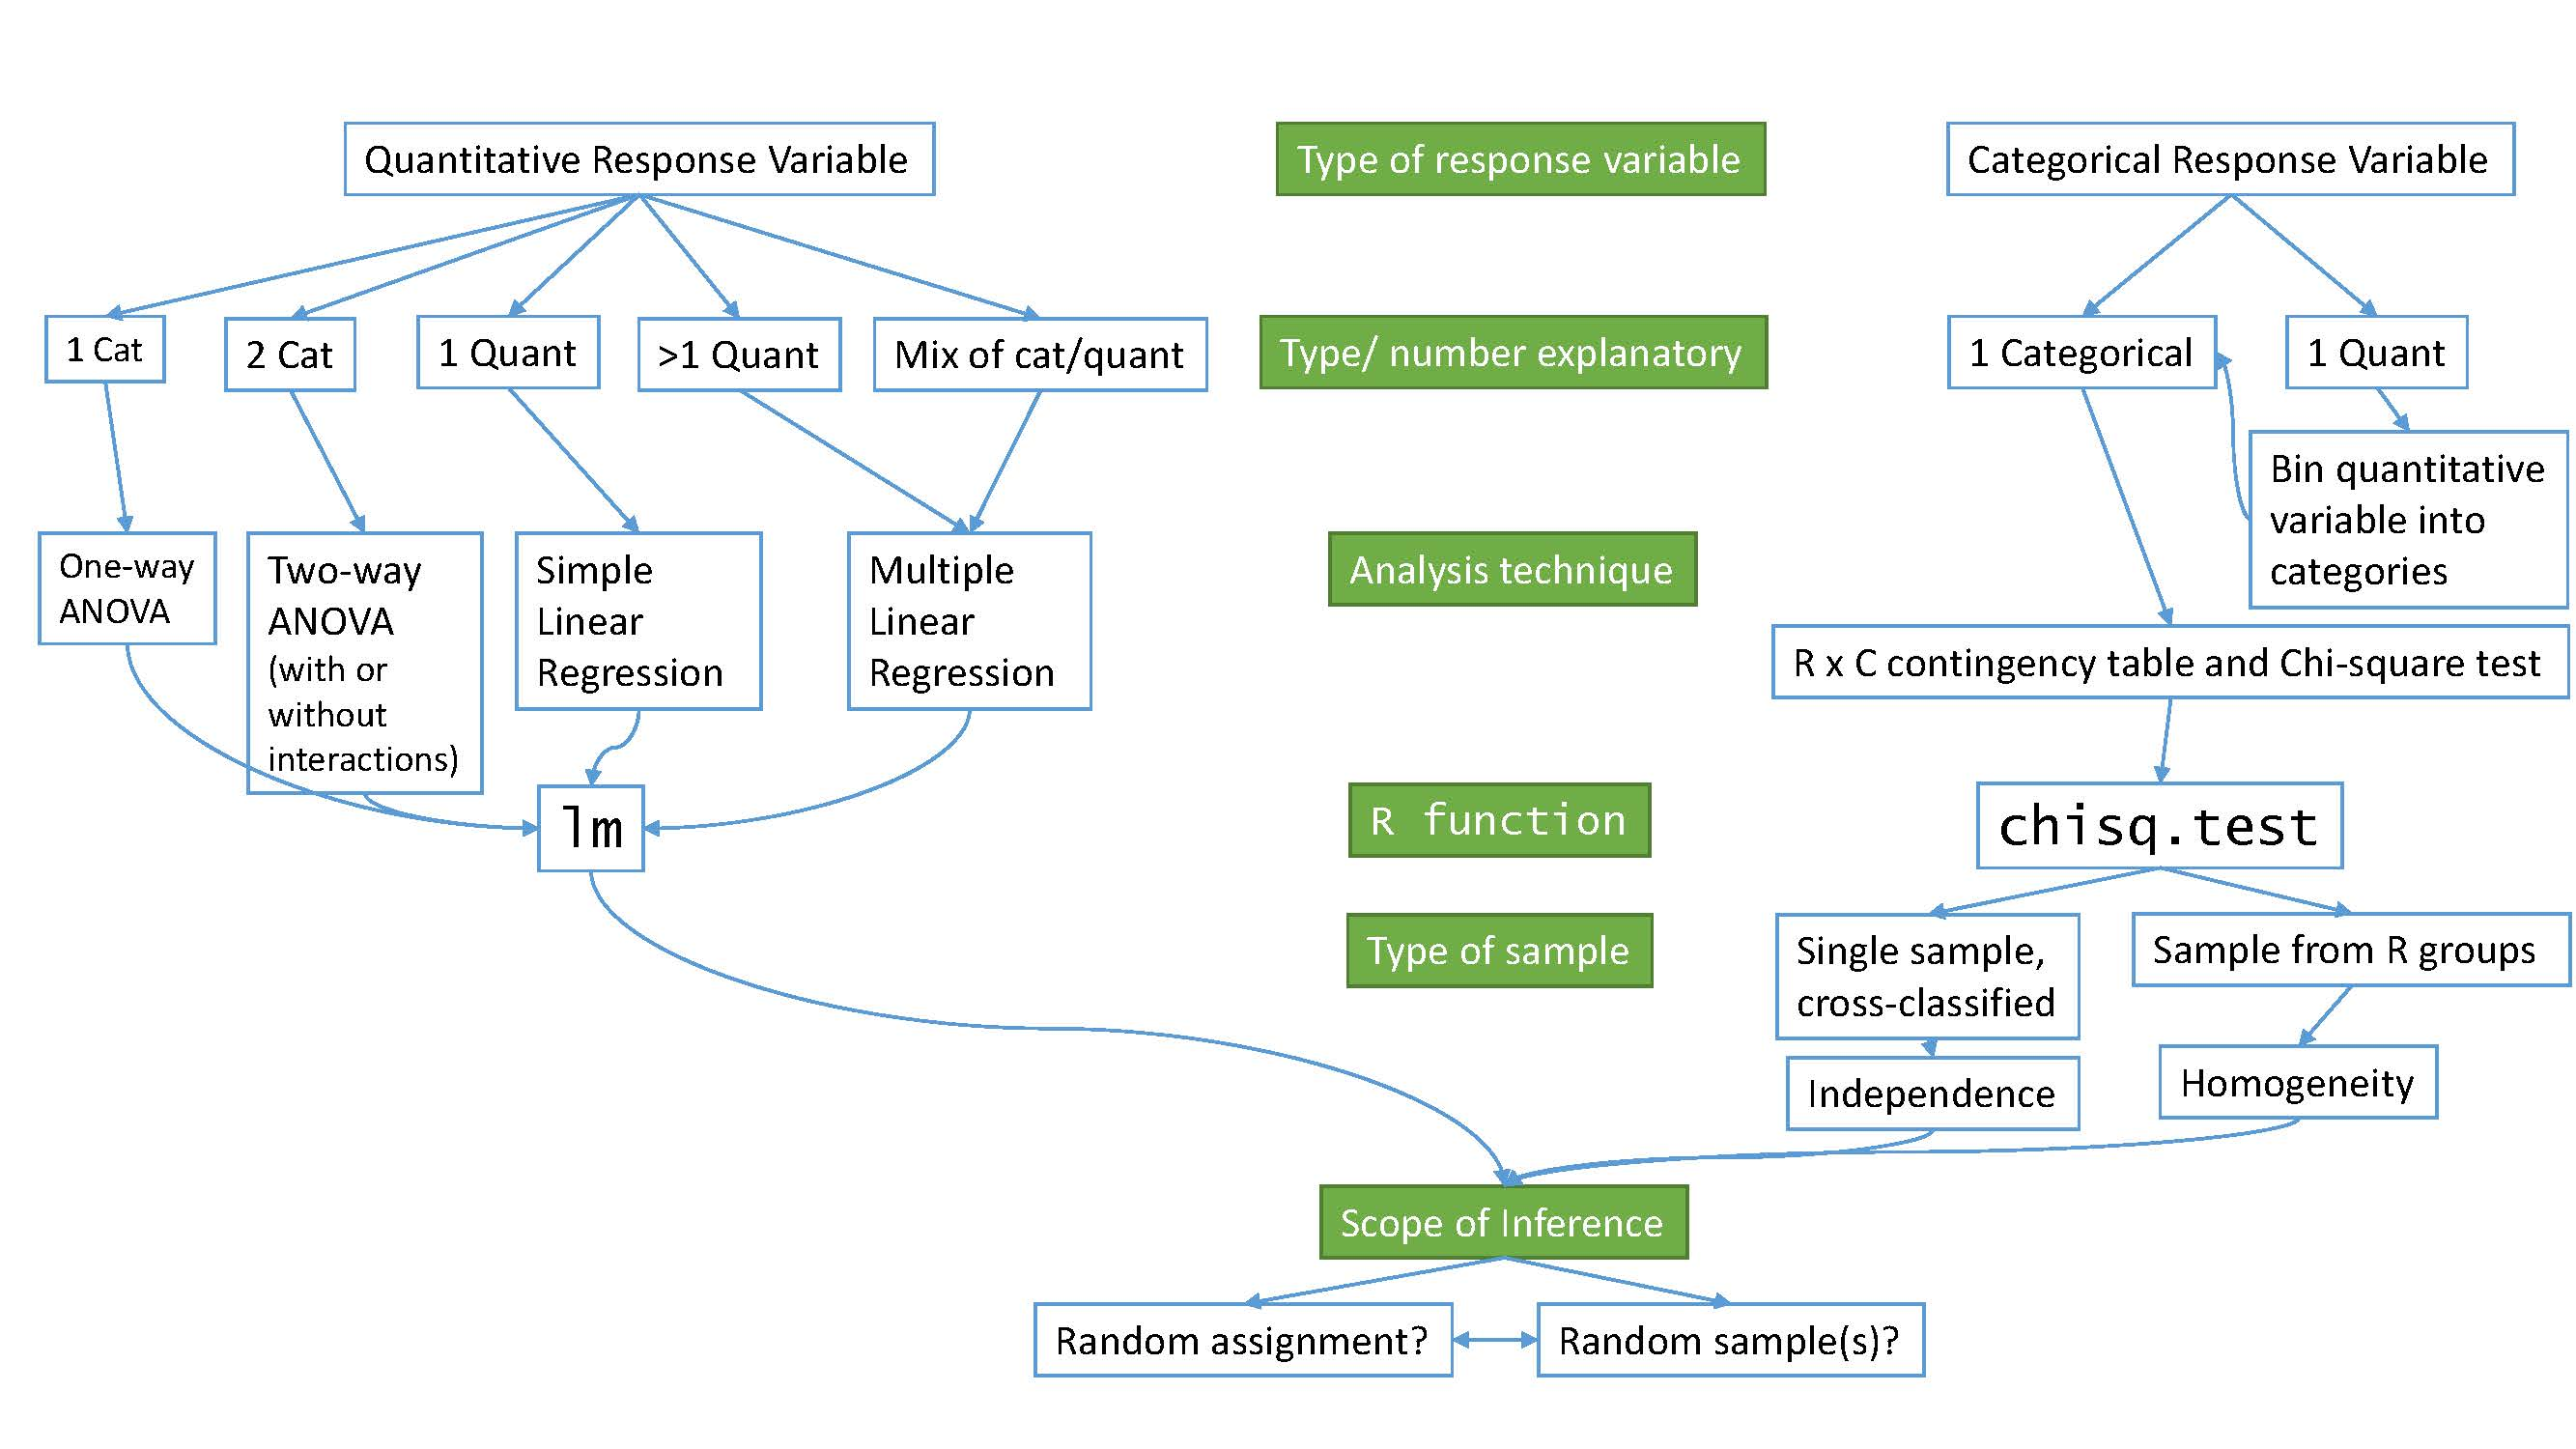
\includegraphics[width=0.75\linewidth]{chapter1_files/decisiontree} 

}

\caption{Flow chart of methods.}\label{fig:Figure1-1}
\end{figure}

\indent We will be spending most of the semester working on methods for quantitative
response variables (the
left side of Figure \ref{fig:Figure1-1} is covered in Chapters \ref{chapter2},
\ref{chapter3}, \ref{chapter4}, \ref{chapter6}, \ref{chapter7}, and
\ref{chapter8}), stepping
over to handle the situation with a categorical response variable in Chapter \ref{chapter5} (right side
of Figure \ref{fig:Figure1-1}).
Chapter \ref{chapter9} contains case studies
illustrating all the methods discussed previously, providing a final opportunity
to explore additional examples that illustrate how finding a
path through Figure \ref{fig:Figure1-1} can lead to the appropriate analysis.

\indent The first topics (Chapters \ref{chapter1}, and \ref{chapter2}) will be more
familiar as we start with single and two group situations
with a quantitative response. In your previous statistics course, you should
have seen methods for estimating and quantifying uncertainty for the mean of a
single group and for differences in the means of two groups. Once we have briefly
reviewed these methods and introduced the statistical software that we will use
throughout the course, we will consider the first new statistical material in
Chapter \ref{chapter3}. It involves the situation with a quantitative response
variable where
there are more than 2 groups to compare -- this is what we call the \textbf{\emph{One-Way
ANOVA}} situation. It generalizes the 2-independent sample hypothesis
test to handle situations where more than 2 groups are being studied. When we
learn this method, we will begin discussing model assumptions \index{assumptions} and methods for
assessing those assumptions that will be present in every analysis involving a
quantitative response. The \textbf{\emph{Two-Way ANOVA}} (Chapter \ref{chapter3})
considers situations with two categorical explanatory variables and a
quantitative response. To make
this somewhat concrete, suppose we are interested in assessing differences in,
say, the \emph{yield} of wheat from a field based on the amount of \emph{fertilizer} applied
(none, low, or high) and \emph{variety} of wheat (two types). Here, \emph{yield} is a quantitative response variable that might be measured in bushels per acre and
there are two categorical explanatory variables, \emph{fertilizer}, with three levels, and \emph{variety}, with two levels. In this material, we introduce the idea of an
\textbf{\emph{interaction}} between the two explanatory variables: \index{interaction!Two-Way ANOVA} the relationship between one categorical
variable and the mean of the response changes depending on the levels of the
other categorical variable. For example, extra fertilizer might enhance the
growth of one variety and hinder the growth of another so we would say that \emph{fertilizer} has different impacts based on the level of \emph{variety}. Given this interaction may or may not actually be present, we will consider two versions of the model in Two-Way ANOVAs, \index{model!Two-Way ANOVA} what are called the \textbf{\emph{additive}} \index{model!additive} (no interaction) and the \textbf{\emph{interaction}} \index{model!interaction} models.

\indent Following the methods for two categorical variables and a quantitative response, we explore a method for
analyzing data where the response is categorical, called the \textbf{\emph{Chi-square test}}
in Chapter \ref{chapter5}. This most closely matches the One-Way ANOVA
situation with a single categorical explanatory variable, except now the
response variable is categorical. For example, we will assess whether taking a
drug (vs taking a \textbf{\emph{placebo}}\footnote{A \textbf{\emph{placebo}} is a treatment level designed to
  mimic the potentially efficacious level(s) but that can have no actual effect. The
  \textbf{\emph{placebo effect}} is the effect that thinking that an effective treatment was
  received has on subjects. There are other related issues in performing experiments
  like the \textbf{\emph{Hawthorne}} or \textbf{\emph{observer effect}} where subjects modify behavior
  because they are being observed.})
has an \textbf{\emph{effect}}\footnote{We will reserve the term ``effect'' for situations where we could
  potentially infer causal impacts on the response of the explanatory variable which
  occurs in situations where the levels of the explanatory variable are randomly
  assigned to the subjects.} on the type of improvement the subjects demonstrate. There
are two different scenarios
for study design that impact the analysis technique and hypotheses tested in
Chapter \ref{chapter5}. If the explanatory variable reflects the group that
subjects were
obtained from, either through randomization of the treatment level to the
subjects or by taking samples from separate populations, this is called a
\textbf{\emph{Chi-square Homogeneity Test}}. \index{Chi-Square Test!Homogeneity Test} It is also possible to obtain a single sample
from a population and then obtain information on the levels of the explanatory
variable for each
subject. We will analyze these results using what is called a \textbf{\emph{Chi-square Independence Test}}.
\index{Chi-Square Test!Independence Test} They both use the same test statistic but we use slightly different graphics and are testing different hypotheses in these two related
situations. Figure \ref{fig:Figure1-1} also shows that if we had a quantitative explanatory
variable and a categorical response that we would need to ``bin'' or create
categories of responses from the quantitative variable to use the Chi-square
testing methods.

\indent If the predictor and response variables are both quantitative, we start with
scatterplots, correlation,
and \textbf{\emph{simple linear regression}} models (Chapters \ref{chapter6} and
\ref{chapter7}) -- things you should have seen, at least to some degree,
previously. The biggest differences here will be
the depth of exploration of diagnostics and inferences for this model and
discussions of transformations of variables. \index{transformation} If there is more than one
explanatory variable, then we say that we are doing \textbf{\emph{multiple linear regression}}
(Chapter \ref{chapter8}) -- the ``multiple'' part of the name reflects that there will
be more
than one explanatory variable. We use the same name if we have a mix of
categorical and quantitative predictor variables but there are some new issues
in setting up the models and interpreting the coefficients that we need to
consider. In the situation with one categorical predictor and one quantitative
predictor, we revisit the idea of an interaction.
\index{interaction!MLR}
It allows us to consider situations
where the estimated relationship between a quantitative predictor and the
mean response
varies among different levels of the categorical variable. In Chapter \ref{chapter9}, connections among all the methods used for quantitative responses are discussed, showing that they are all just linear models \index{model!linear}. We also show how the methods discussed can be applied to a suite of new problems with a set of case studies and how that relates to further extensions of the methods.

\indent By the end of Chapter \ref{chapter9} you should be able to identify, perform
using the statistical software R (\protect\hyperlink{ref-R-base}{R Core Team 2022}), and interpret the results from each of these methods. There
is a lot to learn, but many of the tools for using R and interpreting results
of the analyses accumulate and repeat throughout the textbook. If you work hard to
understand the initial methods, it will help you when the methods get more
complicated. You will likely feel like you are just starting to learn how to
use R at the end of the semester and for learning a new language that is
actually an accomplishment. We will just be taking you on the first steps of a
potentially long journey and it is up to you to decide how much further you
want to go with learning the software.

\indent All the methods you will learn require you to carefully consider how the data were collected, how that
pertains to the population of interest, and how that impacts the inferences
that can be made. The \textbf{\emph{scope of inference}} from the bottom of Figure
\ref{fig:Figure1-1} is our shorthand term for remembering to think about two aspects
of the study -- \textbf{\emph{random assignment}} and \textbf{\emph{random sampling}}.
\index{random assignment} \index{random sampling} In a given
situation, you need to use the description of the study to decide if the
explanatory variable was randomly assigned to study units (this allows for \textbf{\emph{causal inferences}} \index{causal effect} if differences are detected) or not (so no causal statements
are possible). As an example, think about two studies, one where students are
randomly assigned to either get tutoring with their statistics course or not
and another where the students are asked at the end of the semester whether
they sought out tutoring or not. Suppose we compare the final grades in the
course for the two groups (tutoring/not) and find a big difference. In the
first study with random assignment, \index{random assignment} we can say the tutoring caused the
differences we observed. In the second, we could only say that the tutoring was
associated with differences but because students self-selected the group they
ended up in, we can't say that the tutoring caused the differences. The other
aspect of scope of inference concerns random sampling: \index{random sampling} If the data were obtained
using a random sampling mechanism, then our inferences can be safely extended
to the population that the sample was taken from. However, if we have a non-random
sample, our inference can only apply to the sample collected. In the previous
example, the difference would be studying a random sample of students from the
population of, say, Introductory Statistics students at a university versus
studying a sample of students that volunteered for the research project, maybe
for extra credit in the class. We could still randomly assign them to
tutoring/not but the non-random sample would only lead to conclusions about
those students that volunteered. The most powerful scope of inference is when there
are randomly assigned levels of explanatory variables with a random sample from
a population -- conclusions would be about causal impacts that would happen in the
population.

\indent By the end of this material, you should have some basic R skills and abilities to create basic ANOVA and
regression models, as well as to handle Chi-square testing situations.
Together, this should prepare you for future statistics courses or for other
situations where you are expected to be able to identify an appropriate
analysis, do the calculations and required graphics using the data set, and then effectively
communicate interpretations for the methods discussed here.

\hypertarget{section1-2}{%
\section{Getting started in R}\label{section1-2}}

You will need to download the statistical software package called R and an enhanced interface to R called
RStudio (\protect\hyperlink{ref-RStudio}{RStudio Team 2022}). They are open source and free to download and use
(and will always be that way). This means that the skills you learn now can
follow you the rest of your life. R is becoming the primary language of
statistics and is being adopted across academia, government, and businesses to
help manage and learn from the growing volume of data being obtained. Hopefully
you will get a sense of some of the power of R in this book.

\indent The next pages will walk you through the process of getting the software downloaded and provide you with
an initial experience using RStudio to do things that should look familiar
even though the interface will be a new experience. Do not expect to master R
quickly -- it takes years (sorry!) even if you know the statistical methods
being used. We will try to keep all your interactions with R code in a similar
code format and that should help you in learning how to use R as we move
through various methods. We will also often provide you with example code. Everyone
that learns R starts with copying other people's code and then making changes
for specific applications -- so expect to go back to examples from the text and focus
on learning how to modify that code to work for your particular data set. Only
really experienced R users ``know'' functions without having to check other
resources. After we complete this basic introduction, Chapter \ref{chapter2} begins doing
more sophisticated things with R, allowing us to compare quantitative responses
from two groups, make some graphical displays, do hypothesis testing \index{hypothesis testing} and create
confidence intervals in a couple of different ways.

\indent You will have two\footnote{There is a cloud version of R Studio available at \url{https://rstudio.cloud/} that is free for limited usage and some institutions have locally hosted versions that you can use with a web-browser (check with your instructor for those options). We recommend following the steps to be able to work locally but try this option if you have issues with the installation process and need to complete an assignment or two until you get the installation sorted out.} downloading activities to complete before you can do anything
more than read this book\footnote{I created this interactive website (\url{https://rconnect.math.montana.edu/InstallDemo/}) that contains discussions and activities related to installing and using R and RStudio.}. First, you need to download R. It is the engine that will do all the computing
for us, but you will only interact with it once. Go to \url{http://cran.rstudio.com}
and click on the ``\textbf{Download R for\ldots{}}'' button that
corresponds to your operating system. On the next page, click on ``\textbf{base}'' and then it will take you
to a screen to download the most current version of R that is compiled for your
operating system, something like ``\textbf{Download R 4.2.1 for Windows}''. Click on that link and then open
the file you downloaded. You will need to select your preferred language (choose English so your instructor can help you), then hit ``\textbf{Next}''
until it starts to unpack and install the program (all the base settings will be fine). After you hit ``\textbf{Finish}'' you will not do anything further with R directly.

\indent Second, you need to download RStudio. It is an enhanced interface that will make interacting with
R less frustrating and allow you to directly create reports that include the code and output. To download RStudio, go near the bottom of \url{https://www.rstudio.com/products/rstudio/download/} and select the correct version under
``Installers for Supported Platforms'' for your operating system. Download and
then install RStudio using the installer. From this point forward, you should only
open RStudio; it provides your interface with R. Note that both R and RStudio
are updated frequently (up to four times a year) and if you downloaded either
more than a few months previously, you should download the up-to-date versions,
especially if something you are trying to do is not working. Sometimes code
will not work in older versions of R and sometimes old code won't work in new
versions of R.\footnote{The need to keep the code up-to-date as R continues to evolve is
  one reason that this book is locally published and that this is the 9\textsuperscript{th} time
  it has been revised in nine years\ldots{}}



\begin{figure}[ht!]

{\centering 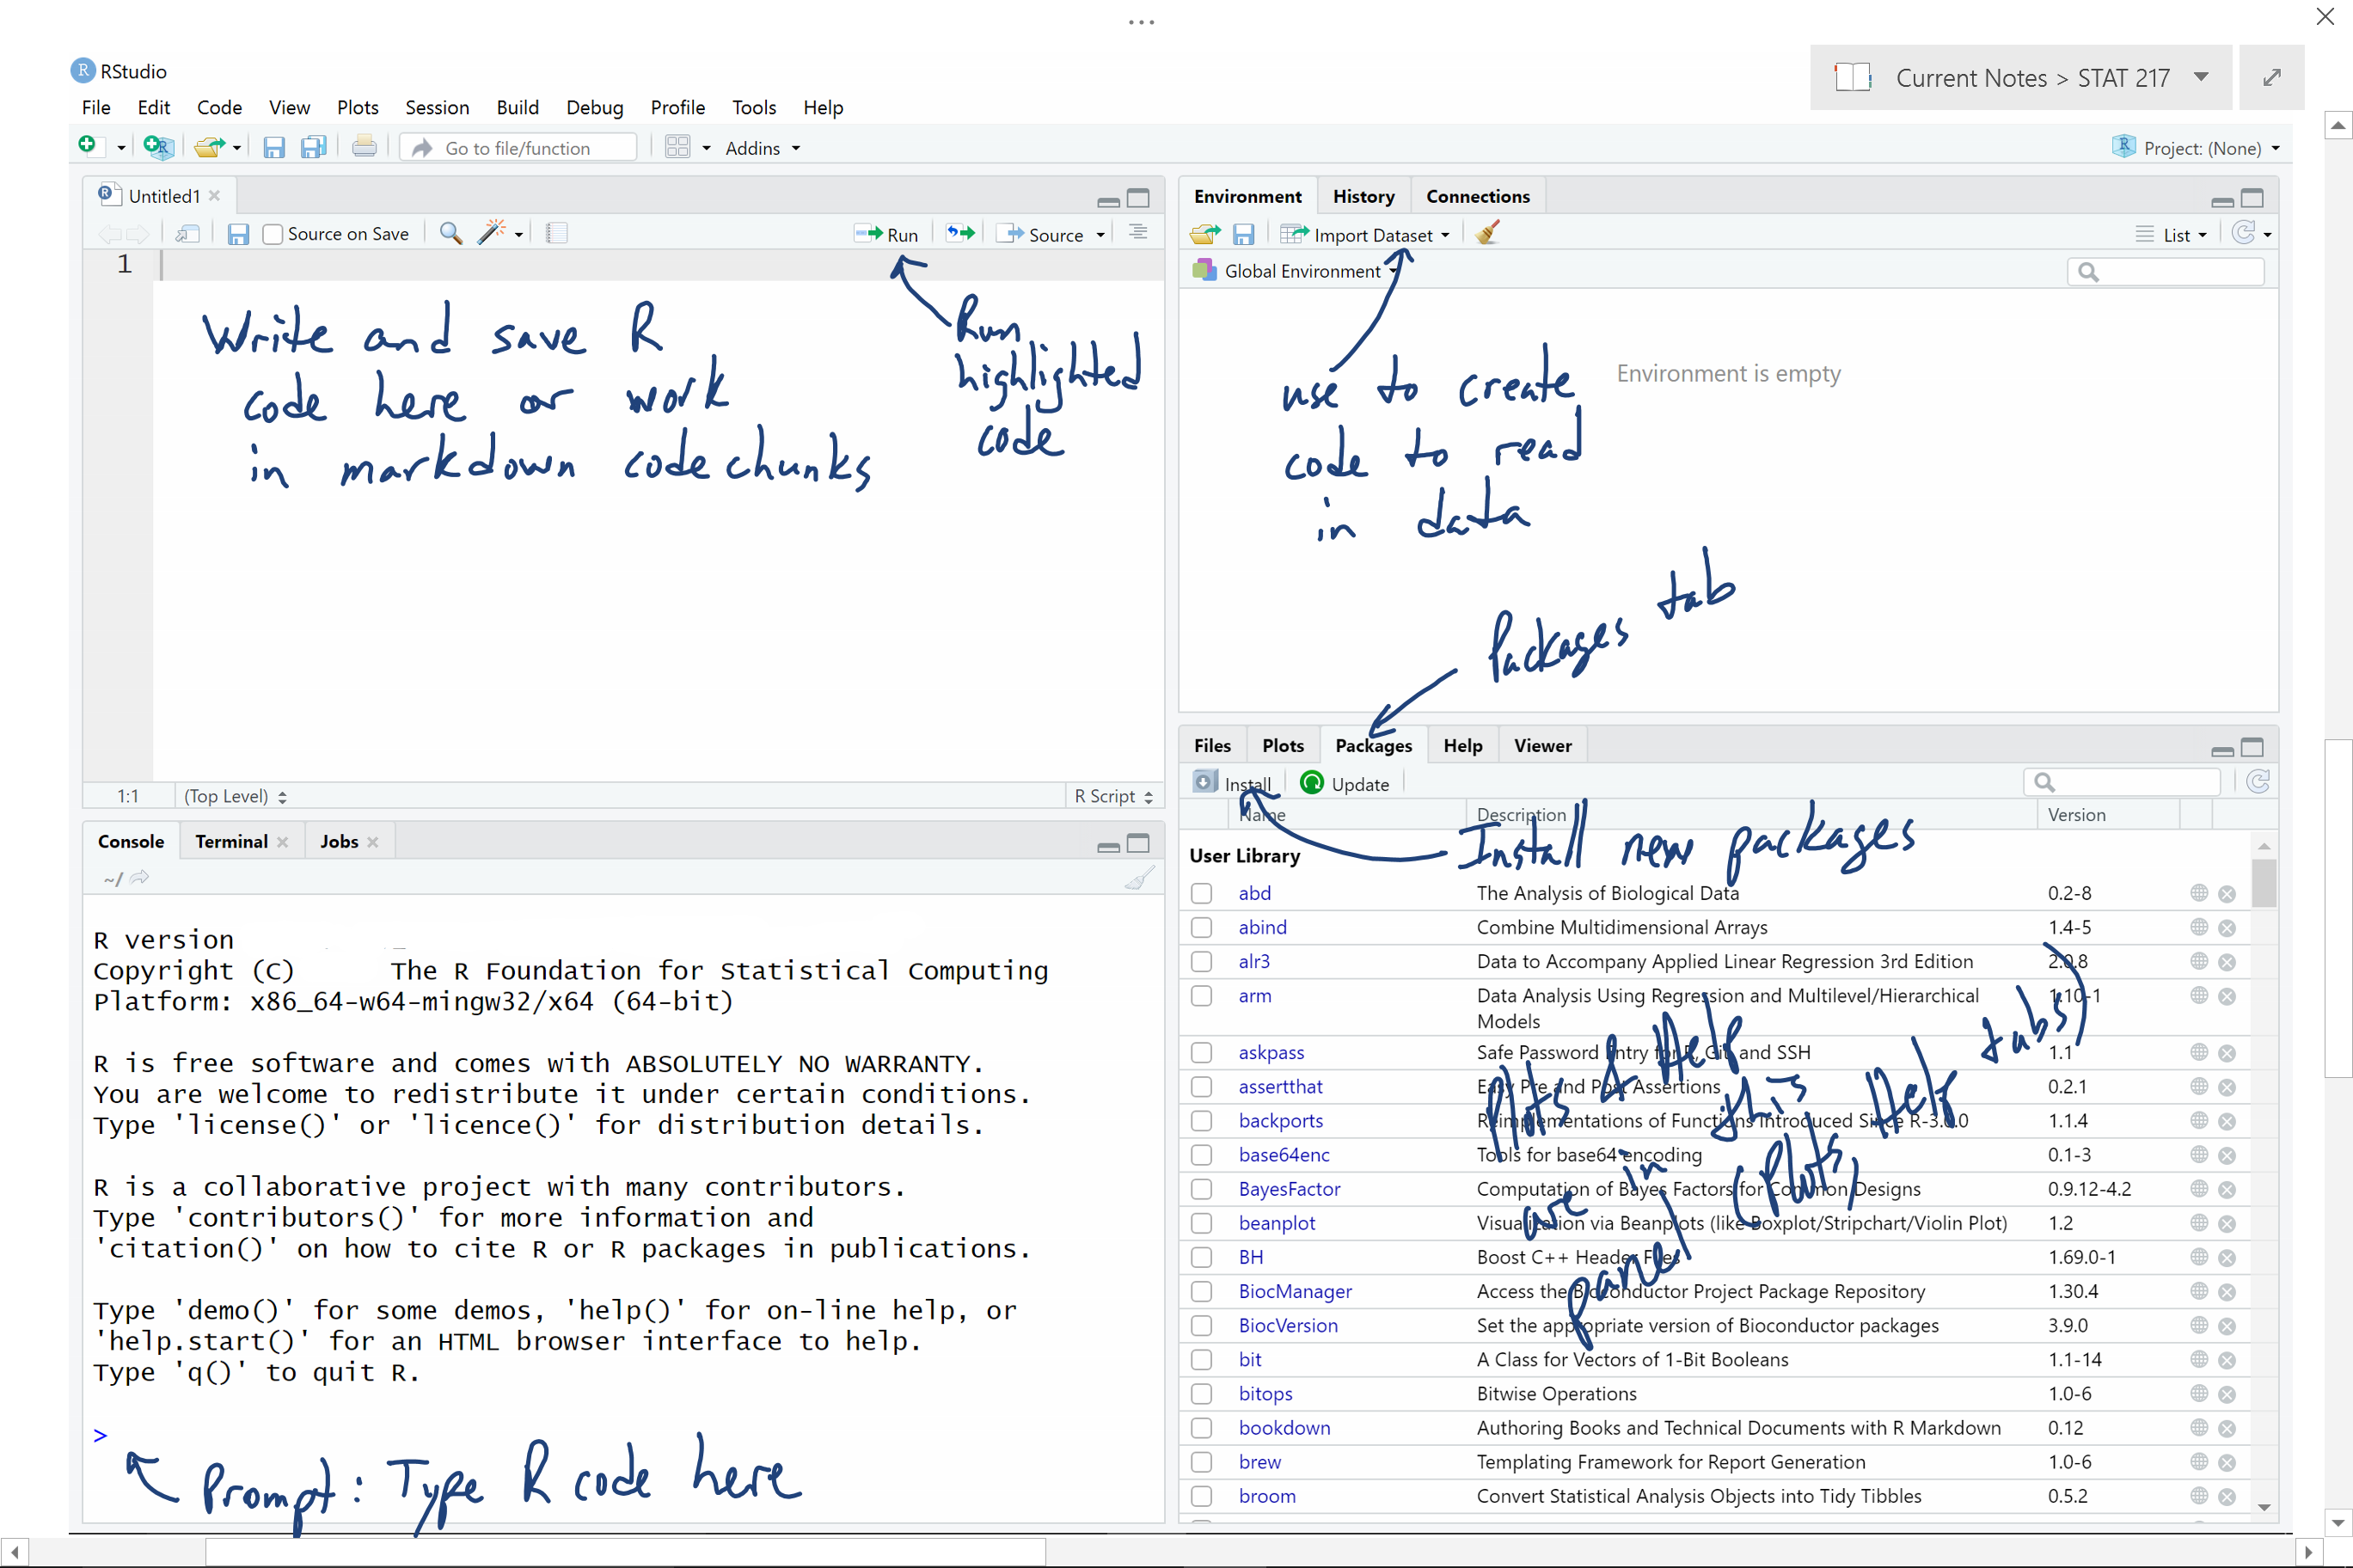
\includegraphics[width=1\linewidth]{chapter1_files/fig1-2} 

}

\caption{Initial RStudio layout.}\label{fig:Figure1-2}
\end{figure}

\newpage

\indent To get started, we can complete some basic tasks in R using the RStudio
interface. When you open RStudio, you will see a screen like Figure
\ref{fig:Figure1-2}. The
added annotation in this and the following screen-grabs is there to help you
get initially oriented to the software interface. R is command-line software --
meaning that in some way or another you have to create code and get it evaluated,
either by entering and execute it at a command prompt or by using the RStudio
interface to run the code that is stored in a file. RStudio makes the management and
execution of that code more efficient than the basic version of R. In RStudio,
the lower left panel is called the ``console'' window and is where you can type R
code directly into R or where you will see the code you run and (most
importantly!) where the results of your executed commands will show up. The
most basic interaction with R is available once you get the cursor active at
the command prompt ``\textgreater{}'' by clicking in that panel (look for a blinking
vertical line). The upper left panel is for writing, saving, and running your R
code either in .R script files or .Rmd (markdown) files, discussed below. Once
you have code available in this window, the ``Run'' button will
execute the code for the line that your cursor is on or for any text that you
have highlighted with your mouse. The ``data management'' or environment panel is
in the upper right, providing information on what data sets have been loaded.
It also contains the ``Import Dataset'' button that provides the easiest way for
you to read a data set into R so you can analyze it. The lower right panel
contains information on the ``Packages'' (additional code we will download and
install to add functionality to R) that are available and is where you will see
plots that you make and requests for ``Help'' on specific functions.

\indent As a first interaction with R we can use it as a calculator. To do this, click near the command prompt
(\texttt{\textgreater{}}) in the lower left ``console'' panel, type 3+4, and then hit enter. It
should look like this:

\begin{Shaded}
\begin{Highlighting}[]
\SpecialCharTok{\textgreater{}} \DecValTok{3} \SpecialCharTok{+} \DecValTok{4}
\NormalTok{[}\DecValTok{1}\NormalTok{] }\DecValTok{7}
\end{Highlighting}
\end{Shaded}

You can do more interesting calculations, like finding the mean of the
numbers -3, 5, 7, and 8 by adding them up and dividing by 4:

\begin{Shaded}
\begin{Highlighting}[]
\SpecialCharTok{\textgreater{}}\NormalTok{ (}\SpecialCharTok{{-}}\DecValTok{3} \SpecialCharTok{+} \DecValTok{5} \SpecialCharTok{+} \DecValTok{7} \SpecialCharTok{+} \DecValTok{8}\NormalTok{)}\SpecialCharTok{/}\DecValTok{4}
\NormalTok{[}\DecValTok{1}\NormalTok{] }\FloatTok{4.25}
\end{Highlighting}
\end{Shaded}

Note that the parentheses help R to figure out your desired order of operations. If you drop that grouping, you get
a very different (and wrong!) result:

\begin{Shaded}
\begin{Highlighting}[]
\SpecialCharTok{\textgreater{}} \SpecialCharTok{{-}}\DecValTok{3} \SpecialCharTok{+} \DecValTok{5} \SpecialCharTok{+} \DecValTok{7} \SpecialCharTok{+} \DecValTok{8}\SpecialCharTok{/}\DecValTok{4}
\NormalTok{[}\DecValTok{1}\NormalTok{] }\DecValTok{11}
\end{Highlighting}
\end{Shaded}

We could estimate the standard deviation similarly using the formula you might remember from introductory
statistics, but that will only work in very limited situations. To use the real
power of R this semester, we need to work with data sets that store the
observations for our subjects in \emph{variables}.
Basically, we need to store observations in named vectors (one dimensional
arrays) that contain a list of the observations. To create a vector containing
the four numbers and assign it to a variable named \emph{variable1}, we need to
create a vector using the concatenate function
\texttt{c} which means ``combine the items'' that follow, if they are inside
parentheses and have commas separating the values,
as follows:

\begin{Shaded}
\begin{Highlighting}[]
\SpecialCharTok{\textgreater{}} \FunctionTok{c}\NormalTok{(}\SpecialCharTok{{-}}\DecValTok{3}\NormalTok{, }\DecValTok{5}\NormalTok{, }\DecValTok{7}\NormalTok{, }\DecValTok{8}\NormalTok{)}
\NormalTok{[}\DecValTok{1}\NormalTok{] }\SpecialCharTok{{-}}\DecValTok{3} \DecValTok{5} \DecValTok{7} \DecValTok{8}
\end{Highlighting}
\end{Shaded}

To get this vector stored in a variable called \emph{variable1} we need to
use the assignment operator, \texttt{\textless{}-} (read as ``is defined to contain'') that assigns
the information on the right into the variable that you are creating on
the left.

\begin{Shaded}
\begin{Highlighting}[]
\SpecialCharTok{\textgreater{}}\NormalTok{ variable1 }\OtherTok{\textless{}{-}} \FunctionTok{c}\NormalTok{(}\SpecialCharTok{{-}}\DecValTok{3}\NormalTok{, }\DecValTok{5}\NormalTok{, }\DecValTok{7}\NormalTok{, }\DecValTok{8}\NormalTok{)}
\end{Highlighting}
\end{Shaded}

In R, the assignment operator, \texttt{\textless{}-}, is created by typing a
``less than'' symbol \texttt{\textless{}} followed by a ``minus'' sign (\texttt{-})
\textbf{without a space between them}. If you
ever want to see what numbers are residing in an object in R, just type
its name and hit \emph{enter}. You can see how that variable contains the same
information that was initially generated by
\texttt{c(-3,\ 5,\ 7,\ 8)} but is easier to access since we just need the text
for the variable name representing that vector.

\begin{Shaded}
\begin{Highlighting}[]
\SpecialCharTok{\textgreater{}}\NormalTok{ variable1}
\NormalTok{[}\DecValTok{1}\NormalTok{] }\SpecialCharTok{{-}}\DecValTok{3} \DecValTok{5} \DecValTok{7} \DecValTok{8}
\end{Highlighting}
\end{Shaded}

With the data stored in a variable, we can use functions such as
\texttt{mean} and
\texttt{sd} to find the mean and standard deviation of the observations contained in
\texttt{variable1}:
\index{mean}
\index{standard deviation}

\begin{Shaded}
\begin{Highlighting}[]
\SpecialCharTok{\textgreater{}} \FunctionTok{mean}\NormalTok{(variable1)}
\NormalTok{[}\DecValTok{1}\NormalTok{] }\FloatTok{4.25}
\SpecialCharTok{\textgreater{}} \FunctionTok{sd}\NormalTok{(variable1)}
\NormalTok{[}\DecValTok{1}\NormalTok{] }\FloatTok{4.99166}
\end{Highlighting}
\end{Shaded}

\indent When dealing with real data, we will often have information about more than one
variable. We could enter all observations by hand for each variable but this is
prone to error and onerous for all but the smallest data sets. If you are to
ever utilize the power of statistics in the evolving data-centered world, data
management has to be accomplished in a more sophisticated way. While you can
manage data sets quite effectively in R, it is often easiest to start with your
data set in something like Microsoft Excel or OpenOffice's Calc. You want to
make sure that observations are in the rows and the names of variables are in
first row of the columns and that there is no ``extra stuff'' in the spreadsheet. If you have
missing observations, they should be represented with blank cells. The file should
be saved as a ``.csv'' file (stands for comma-separated values although Excel
calls it ``CSV (Comma Delimited)''), which basically strips off some of the junk
that Excel adds to the necessary information in the file. Excel will tell you that
this is a bad idea, but it actually creates a more stable archival format and
one that R can use directly.\footnote{There are ways to read ``.xls'' and ``.xlsx'' files
  directly into R that we will explore later so you can also use that format if you prefer.}

\indent The following code to read in the data set relies on an R package called
\texttt{readr} (\protect\hyperlink{ref-R-readr}{Wickham, Hester, and Bryan 2022}). Packages in R provide additional functions and data sets that
are not available in the initial download of R or RStudio. To get access to the packages,
first ``install'' (basically
download) and then ``load'' the package. To install an R package, go to the \textbf{Packages}
tab in the lower right panel of
RStudio. Click on the \textbf{Install} button and then type in the name of the package in
the box (here type in \texttt{readr}).
\index{R packages!\textbf{readr}}
RStudio will try to auto-complete the package name
you are typing which should help you make sure you got it typed correctly. If you are working in a .Rmd file, a highlighted message may show up on the top of the file to suggest packages to install that are not present -- look for this to help make sure you have the needed packages installed. This will
be the first of \emph{many} times that we will mention that R is case sensitive -- in
other words, \texttt{Readr} is different from \texttt{readr} in R syntax and this sort of
thing applies to everything you do in R. You should only need to install each R
package once on a given computer. If you ever see a message that R can't find a
package, make sure it appears in the list in the \textbf{Packages} tab. If it
doesn't, repeat the previous steps to install it.

\begin{longtable}[]{@{}l@{}}
\toprule()
\endhead
\textbf{Important}: R is case sensitive! \texttt{Readr} is not the same as \texttt{readr}! \\
\bottomrule()
\end{longtable}

\newpage

\indent After installing the package, we need to load it to make it active in a given work
session. Go to the command prompt and type (or copy and paste) \texttt{library(readr)} or \texttt{require(readr)}:
\index{R packages!\textbf{readr}}

\begin{verbatim}
> library(readr)
\end{verbatim}

With a data set converted to a CSV file and \texttt{readr} installed and loaded, we need to read the data set into the active workspace.
\index{import data}
There are two ways to do this, either using the point-and-click GUI in RStudio (click
the ``Import Dataset'' button in the upper right ``Environment'' panel as
indicated in Figure \ref{fig:Figure1-2}) or modifying the \texttt{read\_csv}
function to find the file of interest. To practice this, you can
download an Excel (.xls) file from
\url{http://www.math.montana.edu/courses/s217/documents/treadmill.xls}
that contains observations on 31 males that volunteered for a study on methods
for measuring fitness (\protect\hyperlink{ref-Westfall1993}{Westfall and Young 1993}).
In the spreadsheet, you will find a data set that
starts and ends with the following information (only results for Subjects 1, 2,
30, and 31 shown here):

\begin{longtable}[]{@{}
  >{\raggedright\arraybackslash}p{(\columnwidth - 14\tabcolsep) * \real{0.0933}}
  >{\raggedright\arraybackslash}p{(\columnwidth - 14\tabcolsep) * \real{0.1333}}
  >{\raggedright\arraybackslash}p{(\columnwidth - 14\tabcolsep) * \real{0.1733}}
  >{\raggedright\arraybackslash}p{(\columnwidth - 14\tabcolsep) * \real{0.1200}}
  >{\raggedright\arraybackslash}p{(\columnwidth - 14\tabcolsep) * \real{0.1333}}
  >{\raggedright\arraybackslash}p{(\columnwidth - 14\tabcolsep) * \real{0.1067}}
  >{\raggedright\arraybackslash}p{(\columnwidth - 14\tabcolsep) * \real{0.1733}}
  >{\raggedright\arraybackslash}p{(\columnwidth - 14\tabcolsep) * \real{0.0667}}@{}}
\toprule()
\begin{minipage}[b]{\linewidth}\raggedright
Sub-
ject
\end{minipage} & \begin{minipage}[b]{\linewidth}\raggedright
Tread-
MillOx
\end{minipage} & \begin{minipage}[b]{\linewidth}\raggedright
TreadMill-
MaxPulse
\end{minipage} & \begin{minipage}[b]{\linewidth}\raggedright
RunTime
\end{minipage} & \begin{minipage}[b]{\linewidth}\raggedright
RunPulse
\end{minipage} & \begin{minipage}[b]{\linewidth}\raggedright
Rest
Pulse
\end{minipage} & \begin{minipage}[b]{\linewidth}\raggedright
BodyWeight
\end{minipage} & \begin{minipage}[b]{\linewidth}\raggedright
Age
\end{minipage} \\
\midrule()
\endhead
1 & 60.05 & 186 & 8.63 & 170 & 48 & 81.87 & 38 \\
2 & 59.57 & 172 & 8.17 & 166 & 40 & 68.15 & 42 \\
\ldots{} & \ldots{} & \ldots{} & \ldots{} & \ldots{} & \ldots{} & \ldots{} & \ldots{} \\
30 & 39.2 & 172 & 12.88 & 168 & 44 & 91.63 & 54 \\
31 & 37.39 & 192 & 14.03 & 186 & 56 & 87.66 & 45 \\
\bottomrule()
\end{longtable}

\indent The variables contain information on the subject number (\emph{Subject}), subjects'
maximum treadmill oxygen consumption (\emph{TreadMillOx}, in ml per kg per minute, also called maximum VO2) and
maximum pulse rate (\emph{TreadMillMaxPulse}, in beats per minute), time to run 1.5
miles (\emph{Run Time}, in minutes), maximum pulse
during 1.5 mile run (\emph{RunPulse}, in beats per minute), resting pulse rate
(\emph{RestPulse}, beats per minute), Body Weight (\emph{BodyWeight}, in kg), and \emph{Age}
(in years). Open the file in Excel or equivalent software and then save it as
a .csv file in a location you can find on your computer. Then go to RStudio
and click on \textbf{File}, then \textbf{Import Dataset}, then \textbf{From Text (readr)\ldots{}}\footnote{If
  you are having trouble getting the file converted and read into R, copy and
  run the following code:
  \texttt{treadmill\ \textless{}-\ read\_csv("http://www.math.montana.edu/courses/s217/documents/treadmill.csv")}.}
\index{import data}
Click ``\textbf{Import}'' and find your file. R will store the data set as an object with the same name
as the .csv file. You could use another name as well, but it is
often easiest just to keep the data
set name in R related to the original file name. You should see some text appear
in the console (lower left panel) like in Figure \ref{fig:Figure1-3}. The text
that is created
will look something like the following -- if you had stored the file in a drive
labeled D:, it would be:

\begin{Shaded}
\begin{Highlighting}[]
\NormalTok{treadmill }\OtherTok{\textless{}{-}} \FunctionTok{read\_csv}\NormalTok{(}\StringTok{"D:/treadmill.csv"}\NormalTok{)}
\end{Highlighting}
\end{Shaded}

What is put inside the
\texttt{"\ "} will depend on the location and name of your saved .csv file. A
version of the data set in what looks like a
spreadsheet will appear in the upper left window due to the second line of
code (\texttt{View(treadmill})).



\begin{figure}[ht!]

{\centering 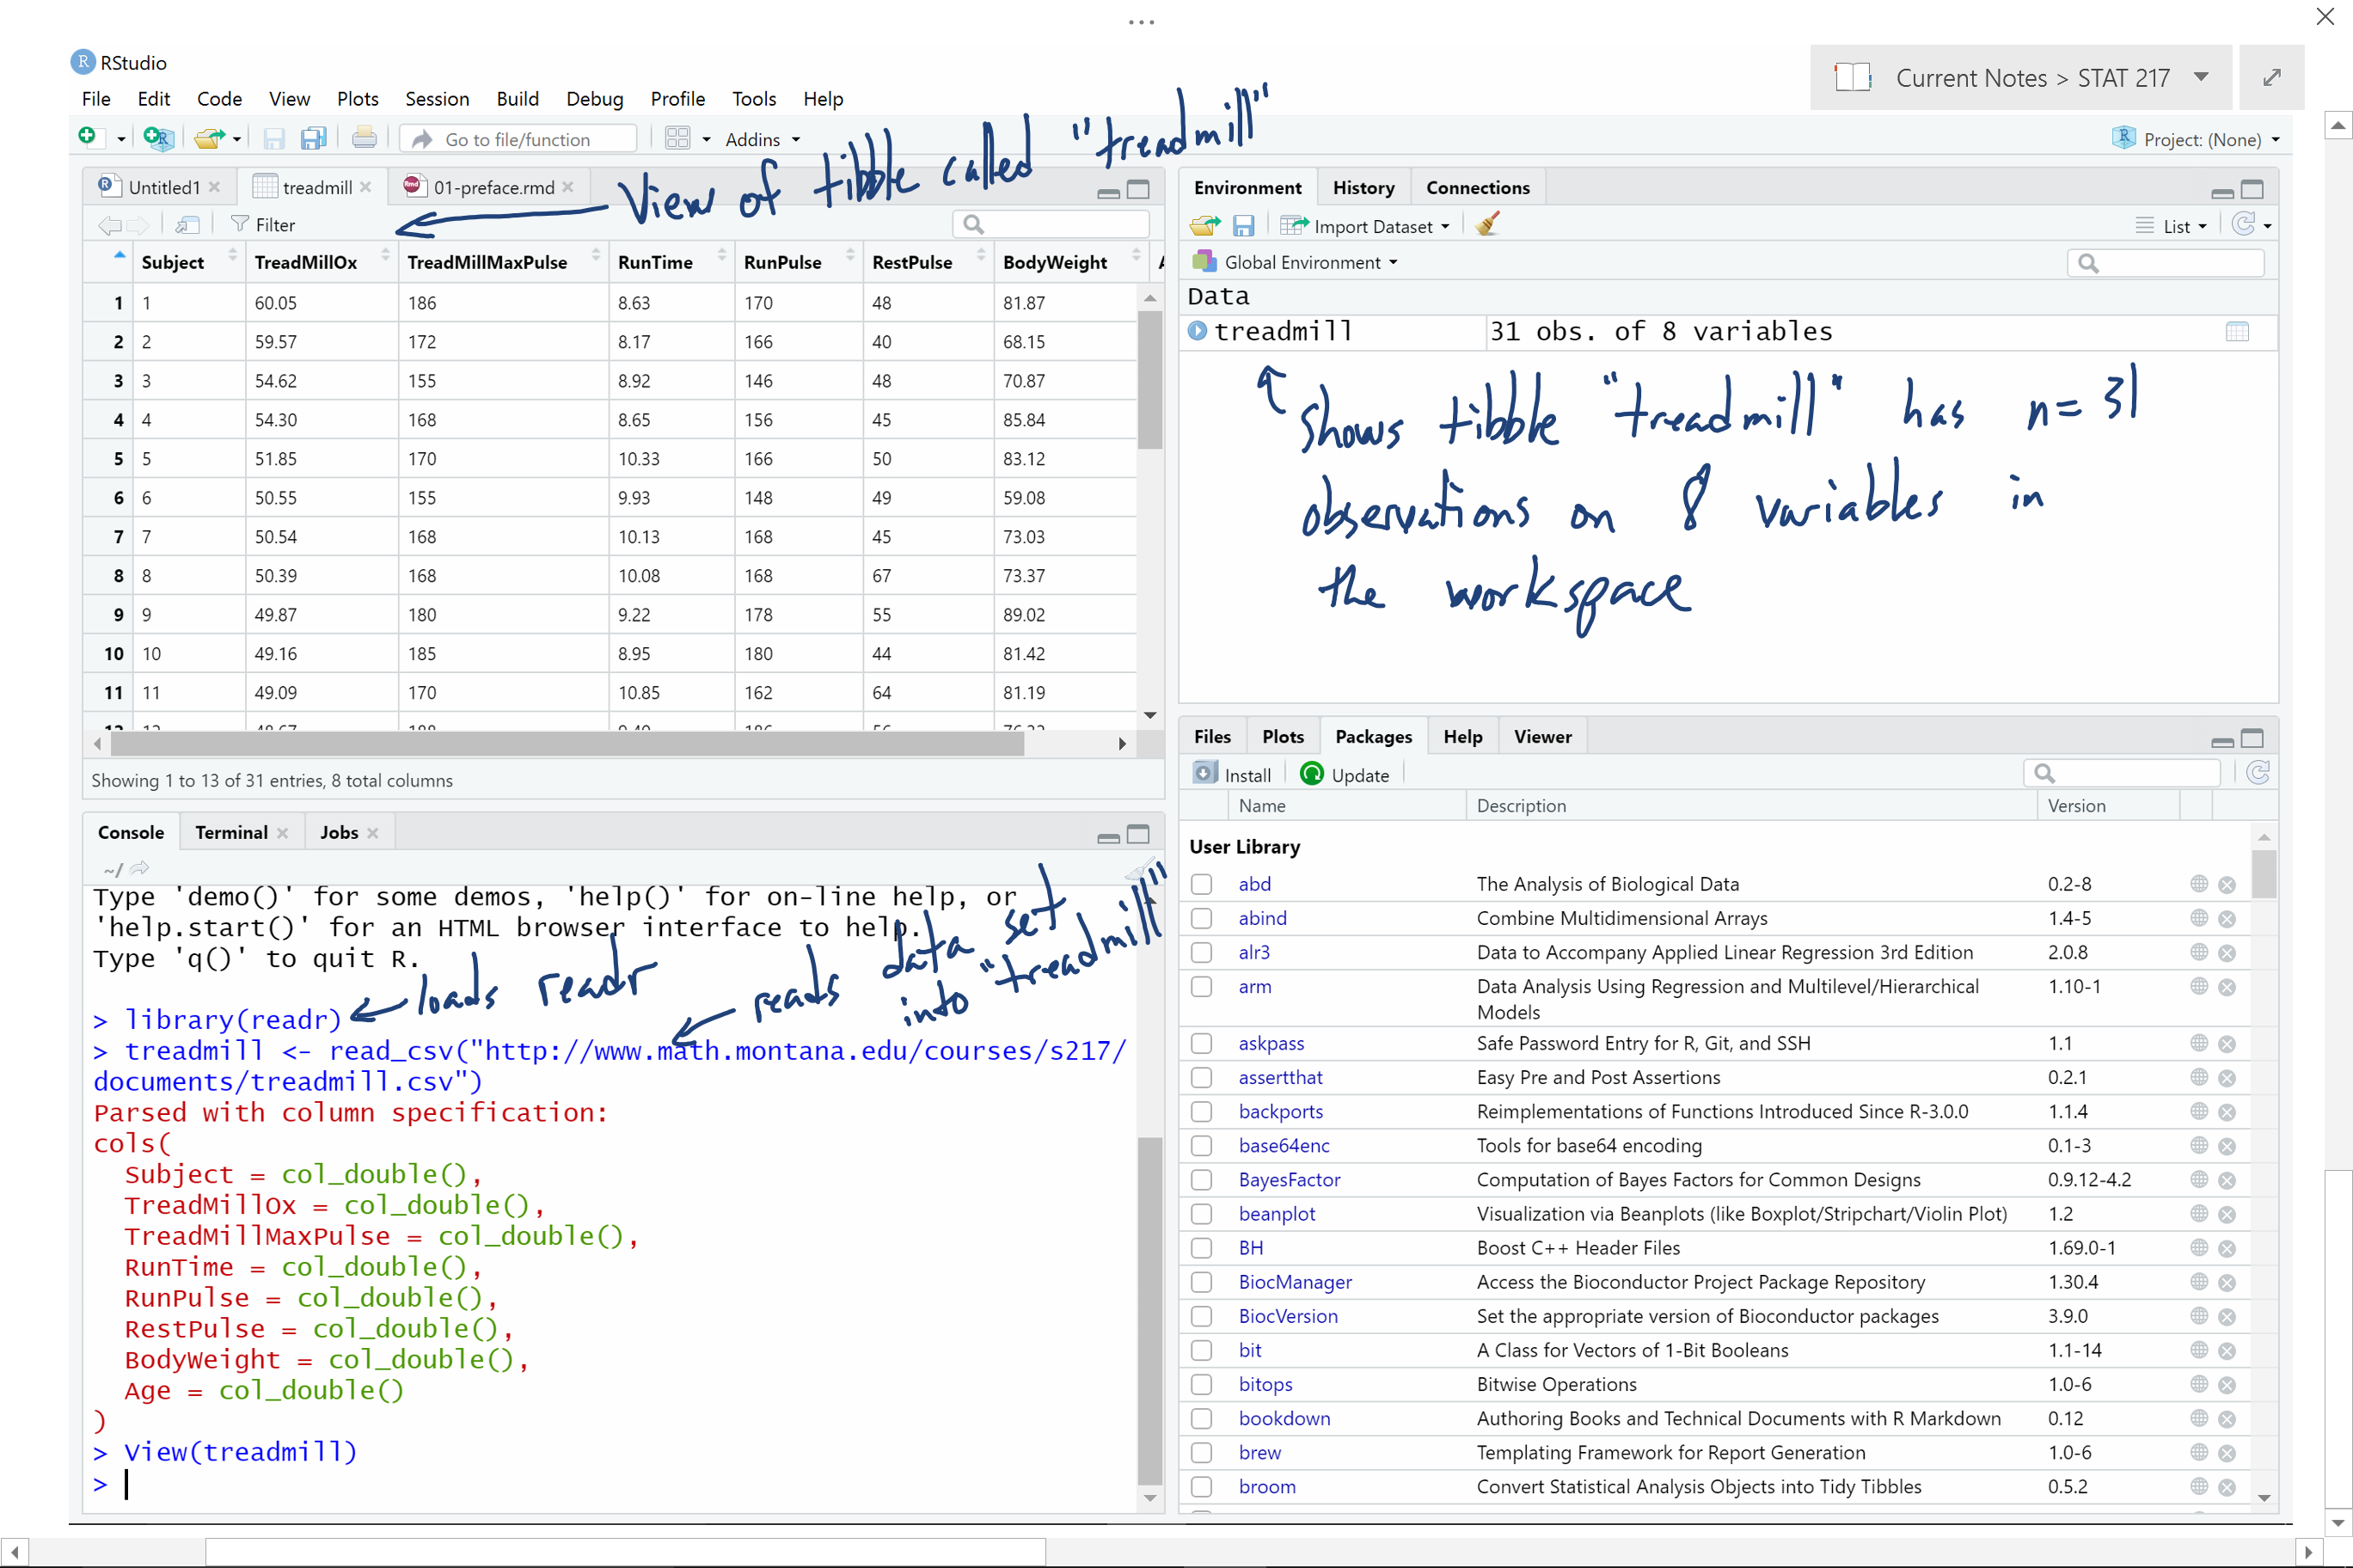
\includegraphics[width=1\linewidth]{chapter1_files/fig1-3} 

}

\caption{RStudio with initial data set loaded.}\label{fig:Figure1-3}
\end{figure}

\indent Just directly typing (or using) a line of code like this is actually the
other way that we can read in
files. If you choose to use the text-only interface, then you need to tell R
where to look in your computer to find the data file. \texttt{read\_csv} is a
function that takes a path as an argument. To use it, specify the path to
your data file, put quotes around it, and put it as the input to
\texttt{read\_csv(...)}. For some examples later in the book, you will be able to
copy a command like this from the text and read data sets and other
code directly from the website, assuming you are connected to the
internet.

\indent To verify that you read the data set in correctly, it is always good to check
its contents. We can view the first and last rows in the data set using the
\texttt{head} and \texttt{tail} functions on the data set, which show the following
results for the
\texttt{treadmill} data. Note that you will sometimes need to resize the console
window in RStudio to get all the columns to display
in a single row which can be performed by dragging the gray bars that separate
the panels.
\index{\texttt{head()}}
\index{\texttt{tail()}}

\small

\begin{Shaded}
\begin{Highlighting}[]
\SpecialCharTok{\textgreater{}} \FunctionTok{head}\NormalTok{(treadmill)}
\CommentTok{\# A tibble: 6 x 8}
\NormalTok{  Subject TreadMillOx TreadMillMaxPulse RunTime RunPulse RestPulse BodyWeight   Age}
    \SpecialCharTok{\textless{}}\NormalTok{int}\SpecialCharTok{\textgreater{}}       \ErrorTok{\textless{}}\NormalTok{dbl}\SpecialCharTok{\textgreater{}}             \ErrorTok{\textless{}}\NormalTok{int}\SpecialCharTok{\textgreater{}}   \ErrorTok{\textless{}}\NormalTok{dbl}\SpecialCharTok{\textgreater{}}    \ErrorTok{\textless{}}\NormalTok{int}\SpecialCharTok{\textgreater{}}     \ErrorTok{\textless{}}\NormalTok{int}\SpecialCharTok{\textgreater{}}      \ErrorTok{\textless{}}\NormalTok{dbl}\SpecialCharTok{\textgreater{}} \ErrorTok{\textless{}}\NormalTok{int}\SpecialCharTok{\textgreater{}}
\DecValTok{1}       \DecValTok{1}       \FloatTok{60.05}               \DecValTok{186}    \FloatTok{8.63}      \DecValTok{170}        \DecValTok{48}      \FloatTok{81.87}    \DecValTok{38}
\DecValTok{2}       \DecValTok{2}       \FloatTok{59.57}               \DecValTok{172}    \FloatTok{8.17}      \DecValTok{166}        \DecValTok{40}      \FloatTok{68.15}    \DecValTok{42}
\DecValTok{3}       \DecValTok{3}       \FloatTok{54.62}               \DecValTok{155}    \FloatTok{8.92}      \DecValTok{146}        \DecValTok{48}      \FloatTok{70.87}    \DecValTok{50}
\DecValTok{4}       \DecValTok{4}       \FloatTok{54.30}               \DecValTok{168}    \FloatTok{8.65}      \DecValTok{156}        \DecValTok{45}      \FloatTok{85.84}    \DecValTok{44}
\DecValTok{5}       \DecValTok{5}       \FloatTok{51.85}               \DecValTok{170}   \FloatTok{10.33}      \DecValTok{166}        \DecValTok{50}      \FloatTok{83.12}    \DecValTok{54}
\DecValTok{6}       \DecValTok{6}       \FloatTok{50.55}               \DecValTok{155}    \FloatTok{9.93}      \DecValTok{148}        \DecValTok{49}      \FloatTok{59.08}    \DecValTok{57}

\SpecialCharTok{\textgreater{}} \FunctionTok{tail}\NormalTok{(treadmill)}
\CommentTok{\# A tibble: 6 x 8}
\NormalTok{  Subject TreadMillOx TreadMillMaxPulse RunTime RunPulse RestPulse BodyWeight   Age}
    \SpecialCharTok{\textless{}}\NormalTok{int}\SpecialCharTok{\textgreater{}}       \ErrorTok{\textless{}}\NormalTok{dbl}\SpecialCharTok{\textgreater{}}             \ErrorTok{\textless{}}\NormalTok{int}\SpecialCharTok{\textgreater{}}   \ErrorTok{\textless{}}\NormalTok{dbl}\SpecialCharTok{\textgreater{}}    \ErrorTok{\textless{}}\NormalTok{int}\SpecialCharTok{\textgreater{}}     \ErrorTok{\textless{}}\NormalTok{int}\SpecialCharTok{\textgreater{}}      \ErrorTok{\textless{}}\NormalTok{dbl}\SpecialCharTok{\textgreater{}} \ErrorTok{\textless{}}\NormalTok{int}\SpecialCharTok{\textgreater{}}
\DecValTok{1}      \DecValTok{26}       \FloatTok{44.61}               \DecValTok{182}   \FloatTok{11.37}      \DecValTok{178}        \DecValTok{62}      \FloatTok{89.47}    \DecValTok{44}
\DecValTok{2}      \DecValTok{27}       \FloatTok{40.84}               \DecValTok{172}   \FloatTok{10.95}      \DecValTok{168}        \DecValTok{57}      \FloatTok{69.63}    \DecValTok{51}
\DecValTok{3}      \DecValTok{28}       \FloatTok{39.44}               \DecValTok{176}   \FloatTok{13.08}      \DecValTok{174}        \DecValTok{63}      \FloatTok{81.42}    \DecValTok{44}
\DecValTok{4}      \DecValTok{29}       \FloatTok{39.41}               \DecValTok{176}   \FloatTok{12.63}      \DecValTok{174}        \DecValTok{58}      \FloatTok{73.37}    \DecValTok{57}
\DecValTok{5}      \DecValTok{30}       \FloatTok{39.20}               \DecValTok{172}   \FloatTok{12.88}      \DecValTok{168}        \DecValTok{44}      \FloatTok{91.63}    \DecValTok{54}
\DecValTok{6}      \DecValTok{31}       \FloatTok{37.39}               \DecValTok{192}   \FloatTok{14.03}      \DecValTok{186}        \DecValTok{56}      \FloatTok{87.66}    \DecValTok{45}
\end{Highlighting}
\end{Shaded}

\normalsize

\newpage

\indent When you load an installed package with \texttt{library}, you may see a warning message about versions of the package and versions of
R -- this is \emph{usually} something you can ignore. Other warning messages could
be more ominous for proceeding but before getting too concerned, there are
couple of basic things to check.
\index{warning message}
First, double check that the package is
installed (see
previous steps). Second, check for typographical errors in your code --
especially for mis-spellings or unintended capitalization. If you are still
having issues, try repeating the installation process. Then click on the ``\textbf{Update}'' button to check for potentially newer versions of packages. If all that fails, try the cloud version of RStudio discussed before and repeat the steps there.

\indent To help you go from basic to intermediate R usage and especially to help with more
complicated problems, you will want to learn how to manage and save your R code.
The best way to do this is using the upper left panel in RStudio. If you just want to manage code, then you can use what
are called R Scripts, which are files that have a file extension of ``.R''. To
start a new ``.R'' file to store your code, click on \textbf{File}, then
\textbf{New File}, then \textbf{R Script}. This will create a blank page to enter and
edit code -- then save the file as something like ``MyFileName.R'' in your preferred location.
Saving your code will mean that you can return to where you
were working last by simply re-running the saved script file. With code in the
script window, you can place the cursor on a line of code or highlight a chunk
of code and hit the ``Run'' button\footnote{You can also use Ctrl+Enter if you like hot keys (Command+Enter on Mac OS).}
on the upper part of the panel. It will appear
in the console with results just like what you would obtain if you typed it
after the command prompt and hit enter for each line. Figure \ref{fig:Figure1-4}
shows the screen with the code used in this
section in the upper left panel, saved in
a file called ``Ch1.R'', with the results of highlighting and executing the first
section of code using the ``Run'' button.



\begin{figure}[ht!]

{\centering 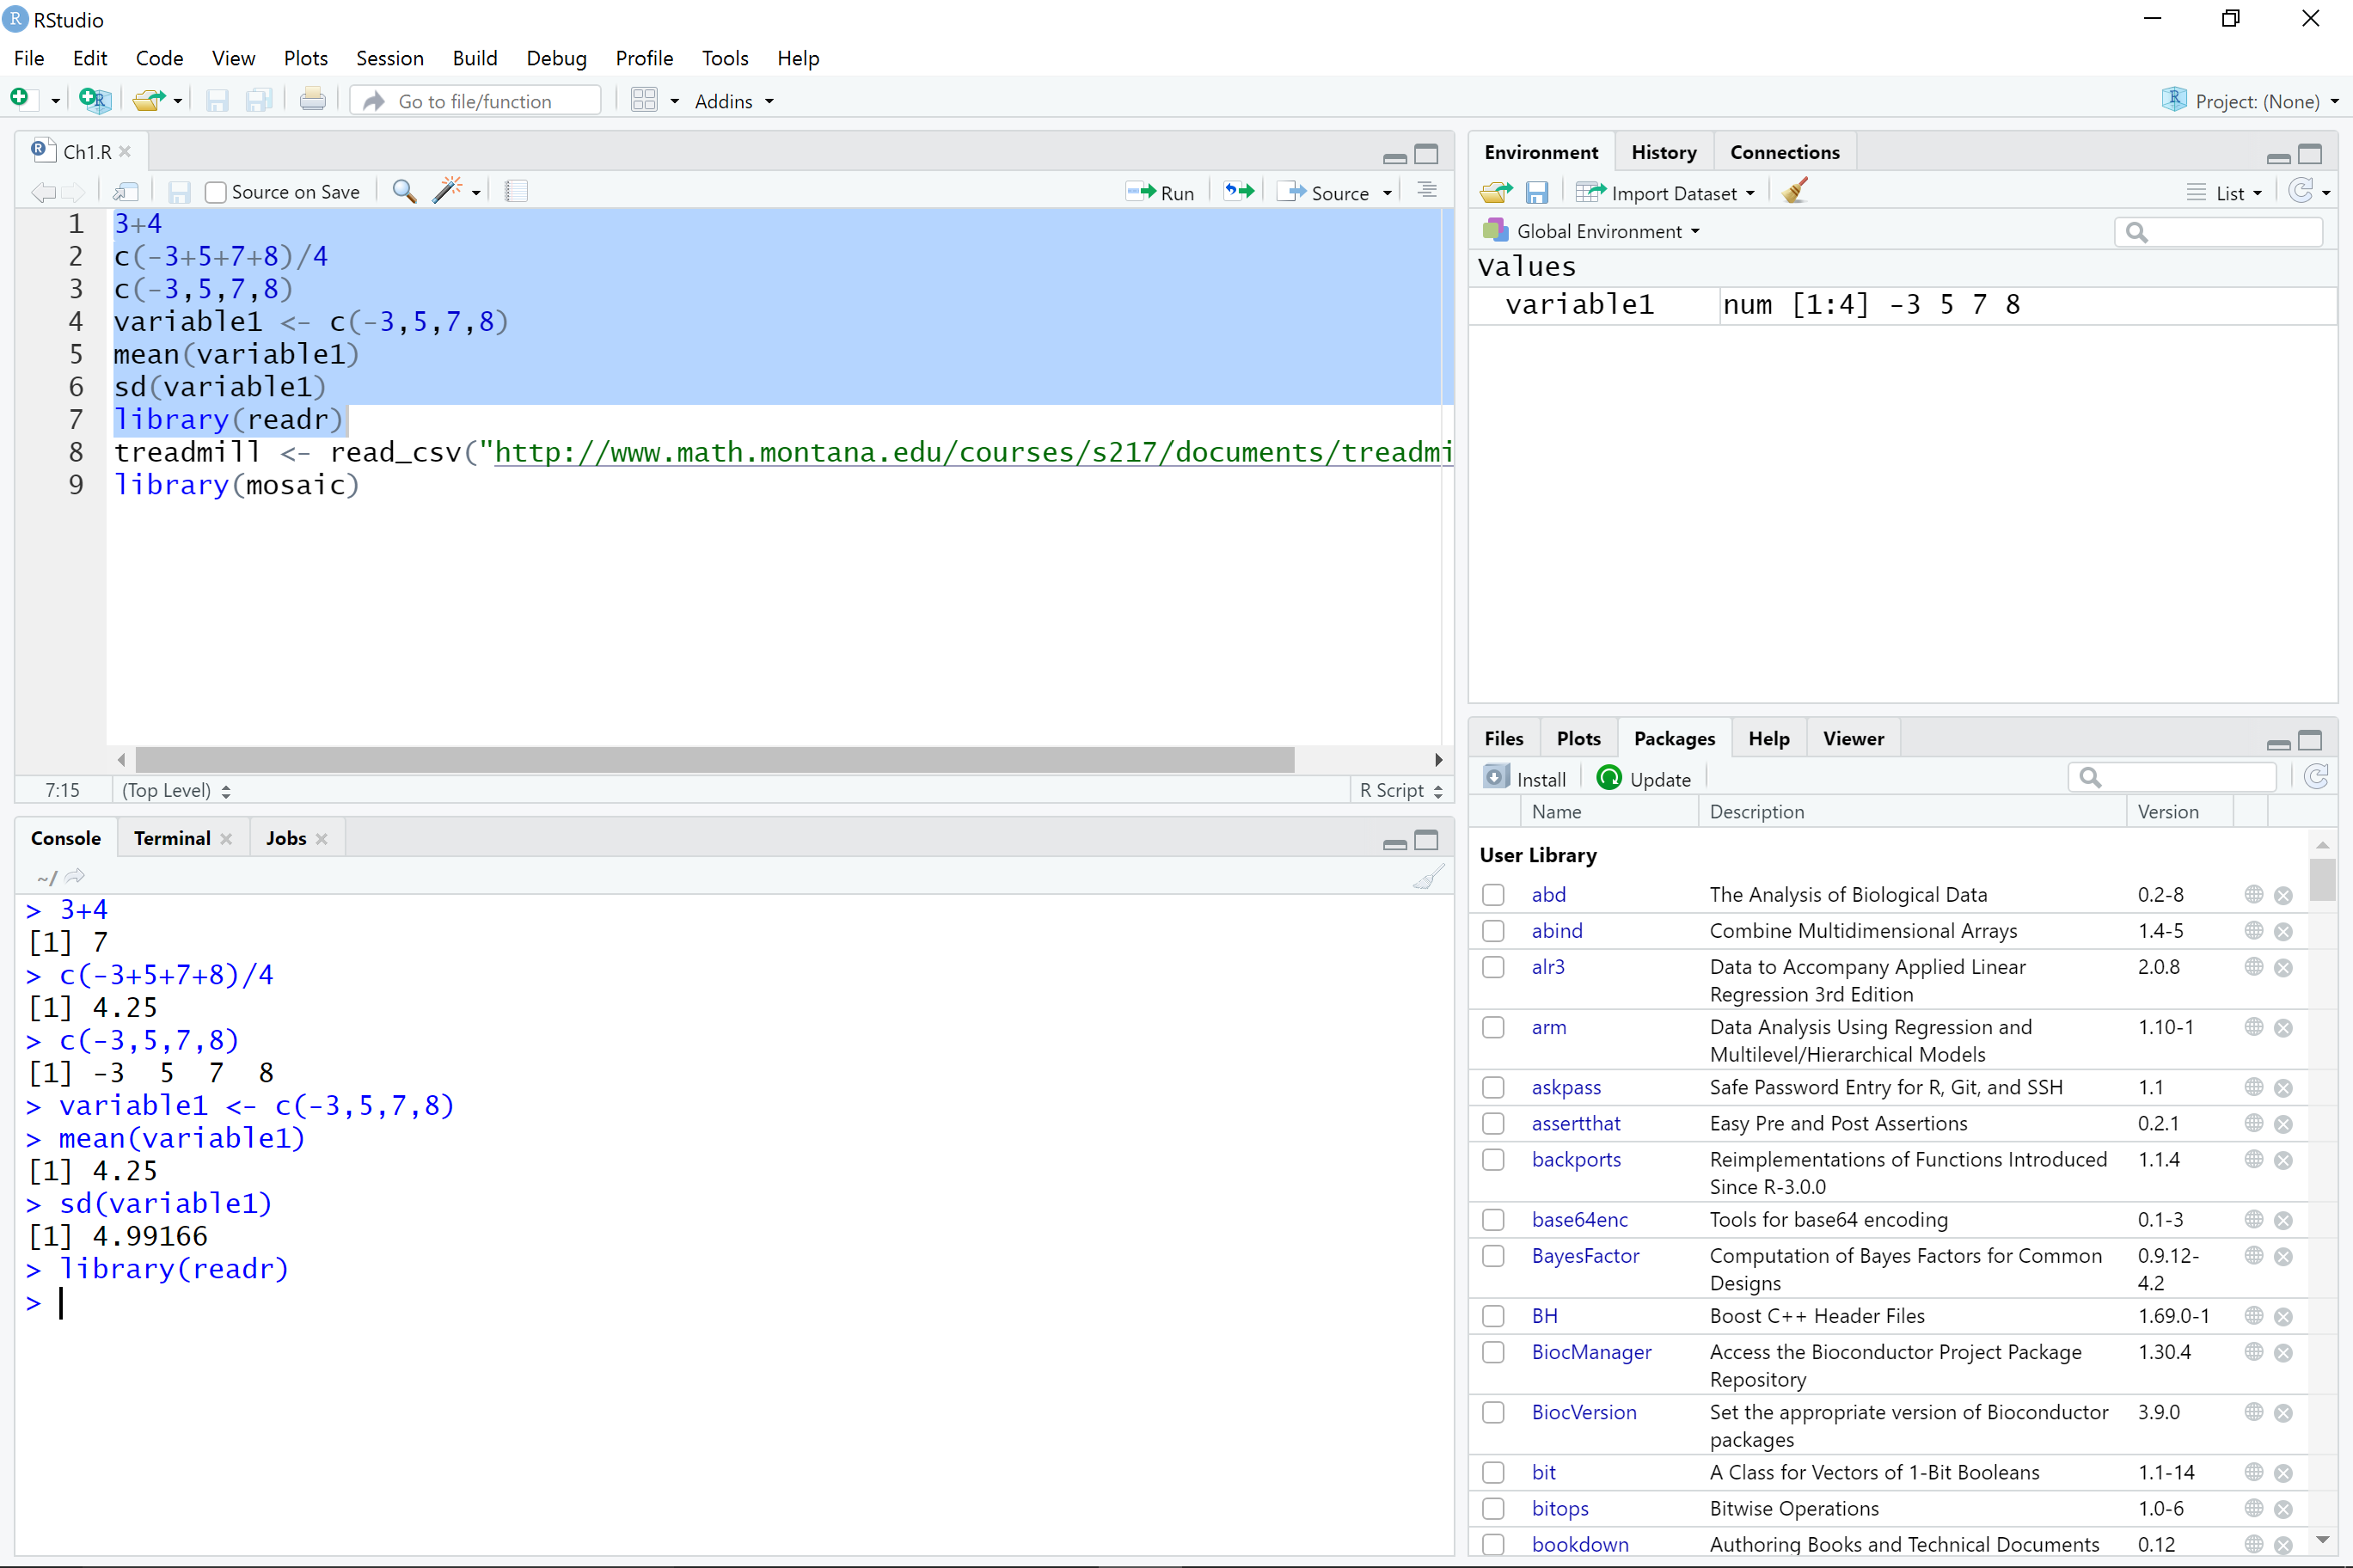
\includegraphics[width=1\linewidth]{chapter1_files/fig1-4} 

}

\caption{RStudio with highlighted code run.}\label{fig:Figure1-4}
\end{figure}

\hypertarget{section1-3}{%
\section{Basic summary statistics, histograms, and boxplots using R}\label{section1-3}}

For the following material, you will need to install and load the \texttt{mosaic} package (\protect\hyperlink{ref-R-mosaic}{Pruim, Kaplan, and Horton 2021a}).

\index{R packages!\textbf{mosaic}}

\begin{Shaded}
\begin{Highlighting}[]
\SpecialCharTok{\textgreater{}} \FunctionTok{library}\NormalTok{(mosaic)}
\end{Highlighting}
\end{Shaded}

It provides a suite of enhanced functions to aid our initial explorations. With RStudio running, the \texttt{mosaic} package loaded, a place to write and
save code, and the \texttt{treadmill} data set loaded, we can (finally!) start to
summarize the results of the study. The \texttt{treadmill} object is what R calls a
\textbf{\emph{tibble}}\footnote{Tibbles are R objects that can contain both
  categorical and quantitative variables on your \(n\) subjects with a name for each
  variable that is also the name of each column in a matrix. \index{tibble} Each subject is a
  row of the data set. The name (supposedly) is due to the way \emph{table} sounds in the accent of a particularly influential developer at RStudio who is from New Zealand.} and contains columns corresponding to each variable in
the spreadsheet. Every
function in R will involve specifying the variable(s) of interest and how you
want to use them. To access a particular variable (column) in a tibble, you
can use a \$ between the name of the tibble and the name of the variable of
interest, generically as \texttt{tibblename\$variablename}. You can think of this as \emph{tibblename's variablename} where the \emph{'s} is replaced by the dollar sign. To identify the
\texttt{RunTime} variable here it would be \texttt{treadmill\$RunTime}. In the command line it would look like:

\begin{Shaded}
\begin{Highlighting}[]
\SpecialCharTok{\textgreater{}}\NormalTok{ treadmill}\SpecialCharTok{$}\NormalTok{RunTime}
\NormalTok{[}\DecValTok{1}\NormalTok{]  }\FloatTok{8.63}  \FloatTok{8.17}  \FloatTok{8.92}  \FloatTok{8.65} \FloatTok{10.33}  \FloatTok{9.93} \FloatTok{10.13} \FloatTok{10.08}  \FloatTok{9.22}  \FloatTok{8.95} \FloatTok{10.85}  \FloatTok{9.40} \FloatTok{11.50} \FloatTok{10.50}
\NormalTok{[}\DecValTok{15}\NormalTok{] }\FloatTok{10.60} \FloatTok{10.25} \FloatTok{10.00} \FloatTok{11.17} \FloatTok{10.47} \FloatTok{11.95}  \FloatTok{9.63} \FloatTok{10.07} \FloatTok{11.08} \FloatTok{11.63} \FloatTok{11.12} \FloatTok{11.37} \FloatTok{10.95} \FloatTok{13.08}
\NormalTok{[}\DecValTok{29}\NormalTok{] }\FloatTok{12.63} \FloatTok{12.88} \FloatTok{14.03}
\end{Highlighting}
\end{Shaded}

\indent Just as in the previous section, we can generate summary statistics using functions like \texttt{mean} and \texttt{sd} by running them on a specific variable:
\index{mean}
\index{standard deviation}

\begin{Shaded}
\begin{Highlighting}[]
\SpecialCharTok{\textgreater{}} \FunctionTok{mean}\NormalTok{(treadmill}\SpecialCharTok{$}\NormalTok{RunTime)}
\NormalTok{[}\DecValTok{1}\NormalTok{] }\FloatTok{10.58613}
\SpecialCharTok{\textgreater{}} \FunctionTok{sd}\NormalTok{(treadmill}\SpecialCharTok{$}\NormalTok{RunTime)}
\NormalTok{[}\DecValTok{1}\NormalTok{] }\FloatTok{1.387414}
\end{Highlighting}
\end{Shaded}

And now we know that the average running time for 1.5 miles for the subjects in the study was 10.6 minutes with a standard deviation (SD) of 1.39 minutes. But you should remember that the
mean and SD are only appropriate summaries if the distribution is roughly
\textbf{\emph{symmetric}} (both sides of the distribution are approximately the same shape and length). The
\texttt{mosaic} package provides a useful function called \texttt{favstats} that provides
the mean and SD as well as the \textbf{\emph{5 number summary}}: \index{5 number summary}
the minimum (\texttt{min}), the first quartile (\texttt{Q1}, the 25\textsuperscript{th} percentile),
the median (50\textsuperscript{th} percentile), the third quartile (\texttt{Q3}, the 75\textsuperscript{th}
percentile), and the maximum (\texttt{max}). It also provides the number of
observations (\texttt{n}) which was 31, as noted above, and a count of whether any
missing values were encountered (\texttt{missing}), which was 0 here since all
subjects had measurements available on this variable.
\index{favstats}

\begin{Shaded}
\begin{Highlighting}[]
\SpecialCharTok{\textgreater{}} \FunctionTok{favstats}\NormalTok{(treadmill}\SpecialCharTok{$}\NormalTok{RunTime)}
\NormalTok{  min   Q1 median    Q3   max     mean       sd  n missing}
 \FloatTok{8.17} \FloatTok{9.78}  \FloatTok{10.47} \FloatTok{11.27} \FloatTok{14.03} \FloatTok{10.58613} \FloatTok{1.387414} \DecValTok{31}       \DecValTok{0}
\end{Highlighting}
\end{Shaded}

\indent We are starting to get somewhere with understanding that the runners were
somewhat fit with the worst runner covering 1.5 miles in 14 minutes
(the equivalent of a 9.3 minute mile)
and the best running at a 5.4 minute mile pace. The limited variation in the
results suggests that the sample was obtained from a restricted group with
somewhat common characteristics. When you explore the ages and weights of the
subjects in the Practice Problems in Section \ref{section1-6}, you will get even more
information about how similar all the subjects in this study were. Researchers often publish numerical summaries of this sort of demographic information to help readers understand the subjects that they studied and that their results might apply to.

\indent A graphical display of these results will help us to assess the shape
of the distribution of run times -- including considering the potential for the presence of a \textbf{\emph{skew}} (whether the right or left tail of the distribution
is noticeably more spread out, with left skew meaning that the left tail
is more spread out than the right tail) \index{skew} and \textbf{\emph{outliers}} \index{outlier}
(unusual observations). A \textbf{\emph{histogram}} \index{histogram} is a good place to start.
Histograms display connected bars with counts of observations defining
the height of bars based on a set of bins of values of the quantitative variable.
We will apply the \texttt{hist} function to the \texttt{RunTime} variable, which produces
Figure \ref{fig:Figure1-5}.

\begin{Shaded}
\begin{Highlighting}[]
\SpecialCharTok{\textgreater{}} \FunctionTok{hist}\NormalTok{(treadmill}\SpecialCharTok{$}\NormalTok{RunTime)}
\end{Highlighting}
\end{Shaded}



\begin{figure}[ht!]

{\centering 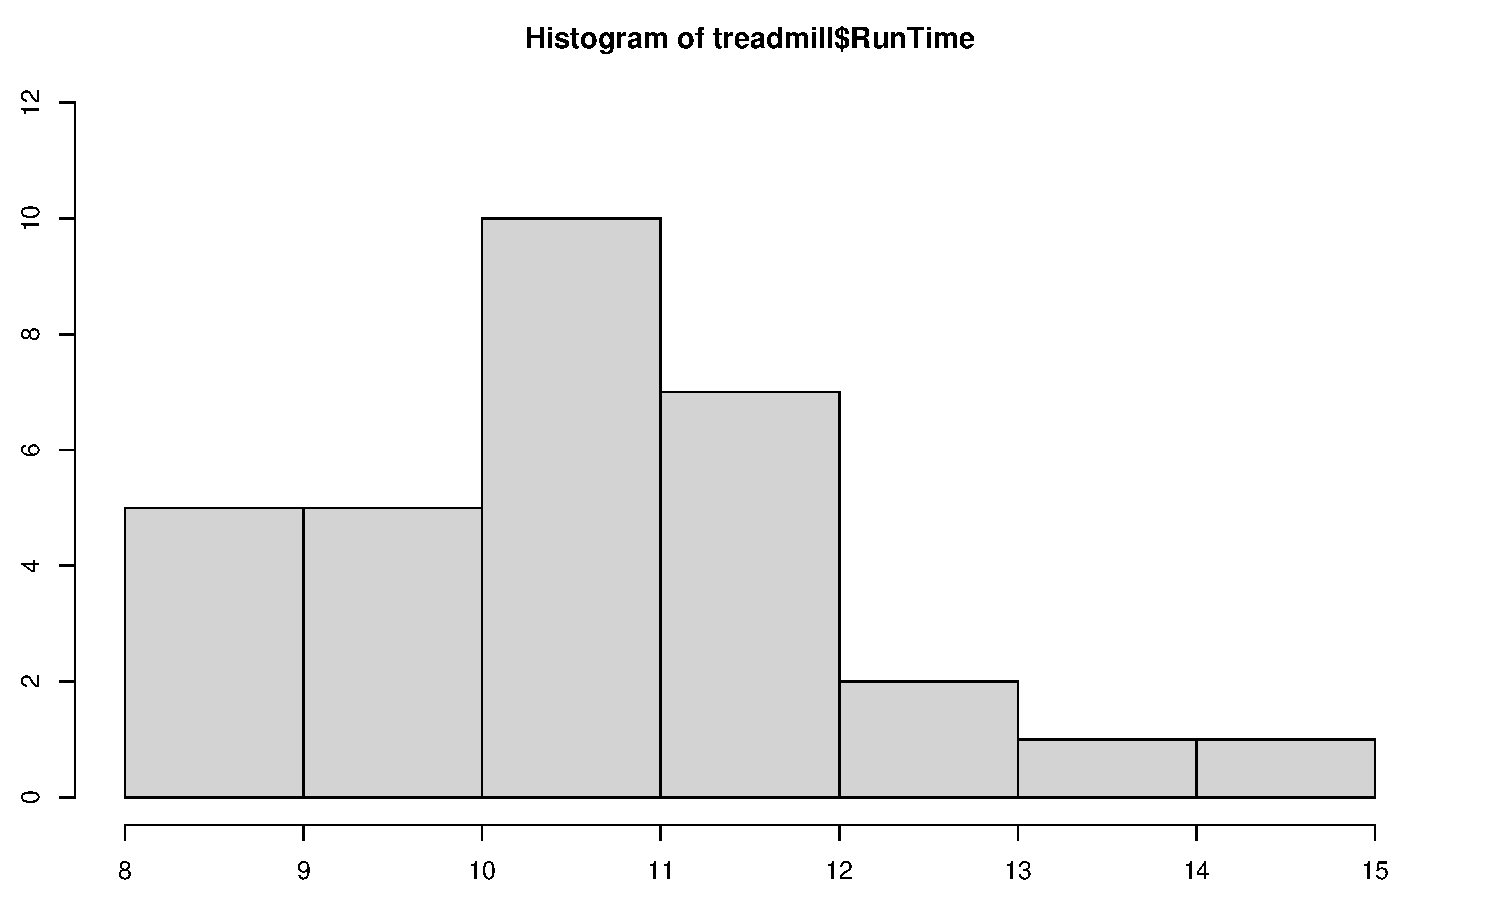
\includegraphics[width=0.75\linewidth]{01-preface_files/figure-latex/Figure1-5-1} 

}

\caption{Histogram of Run Times (minutes) of \(n\) = 31 subjects in Treadmill study, bar heights are counts.}\label{fig:Figure1-5}
\end{figure}



\begin{figure}[ht!]

{\centering 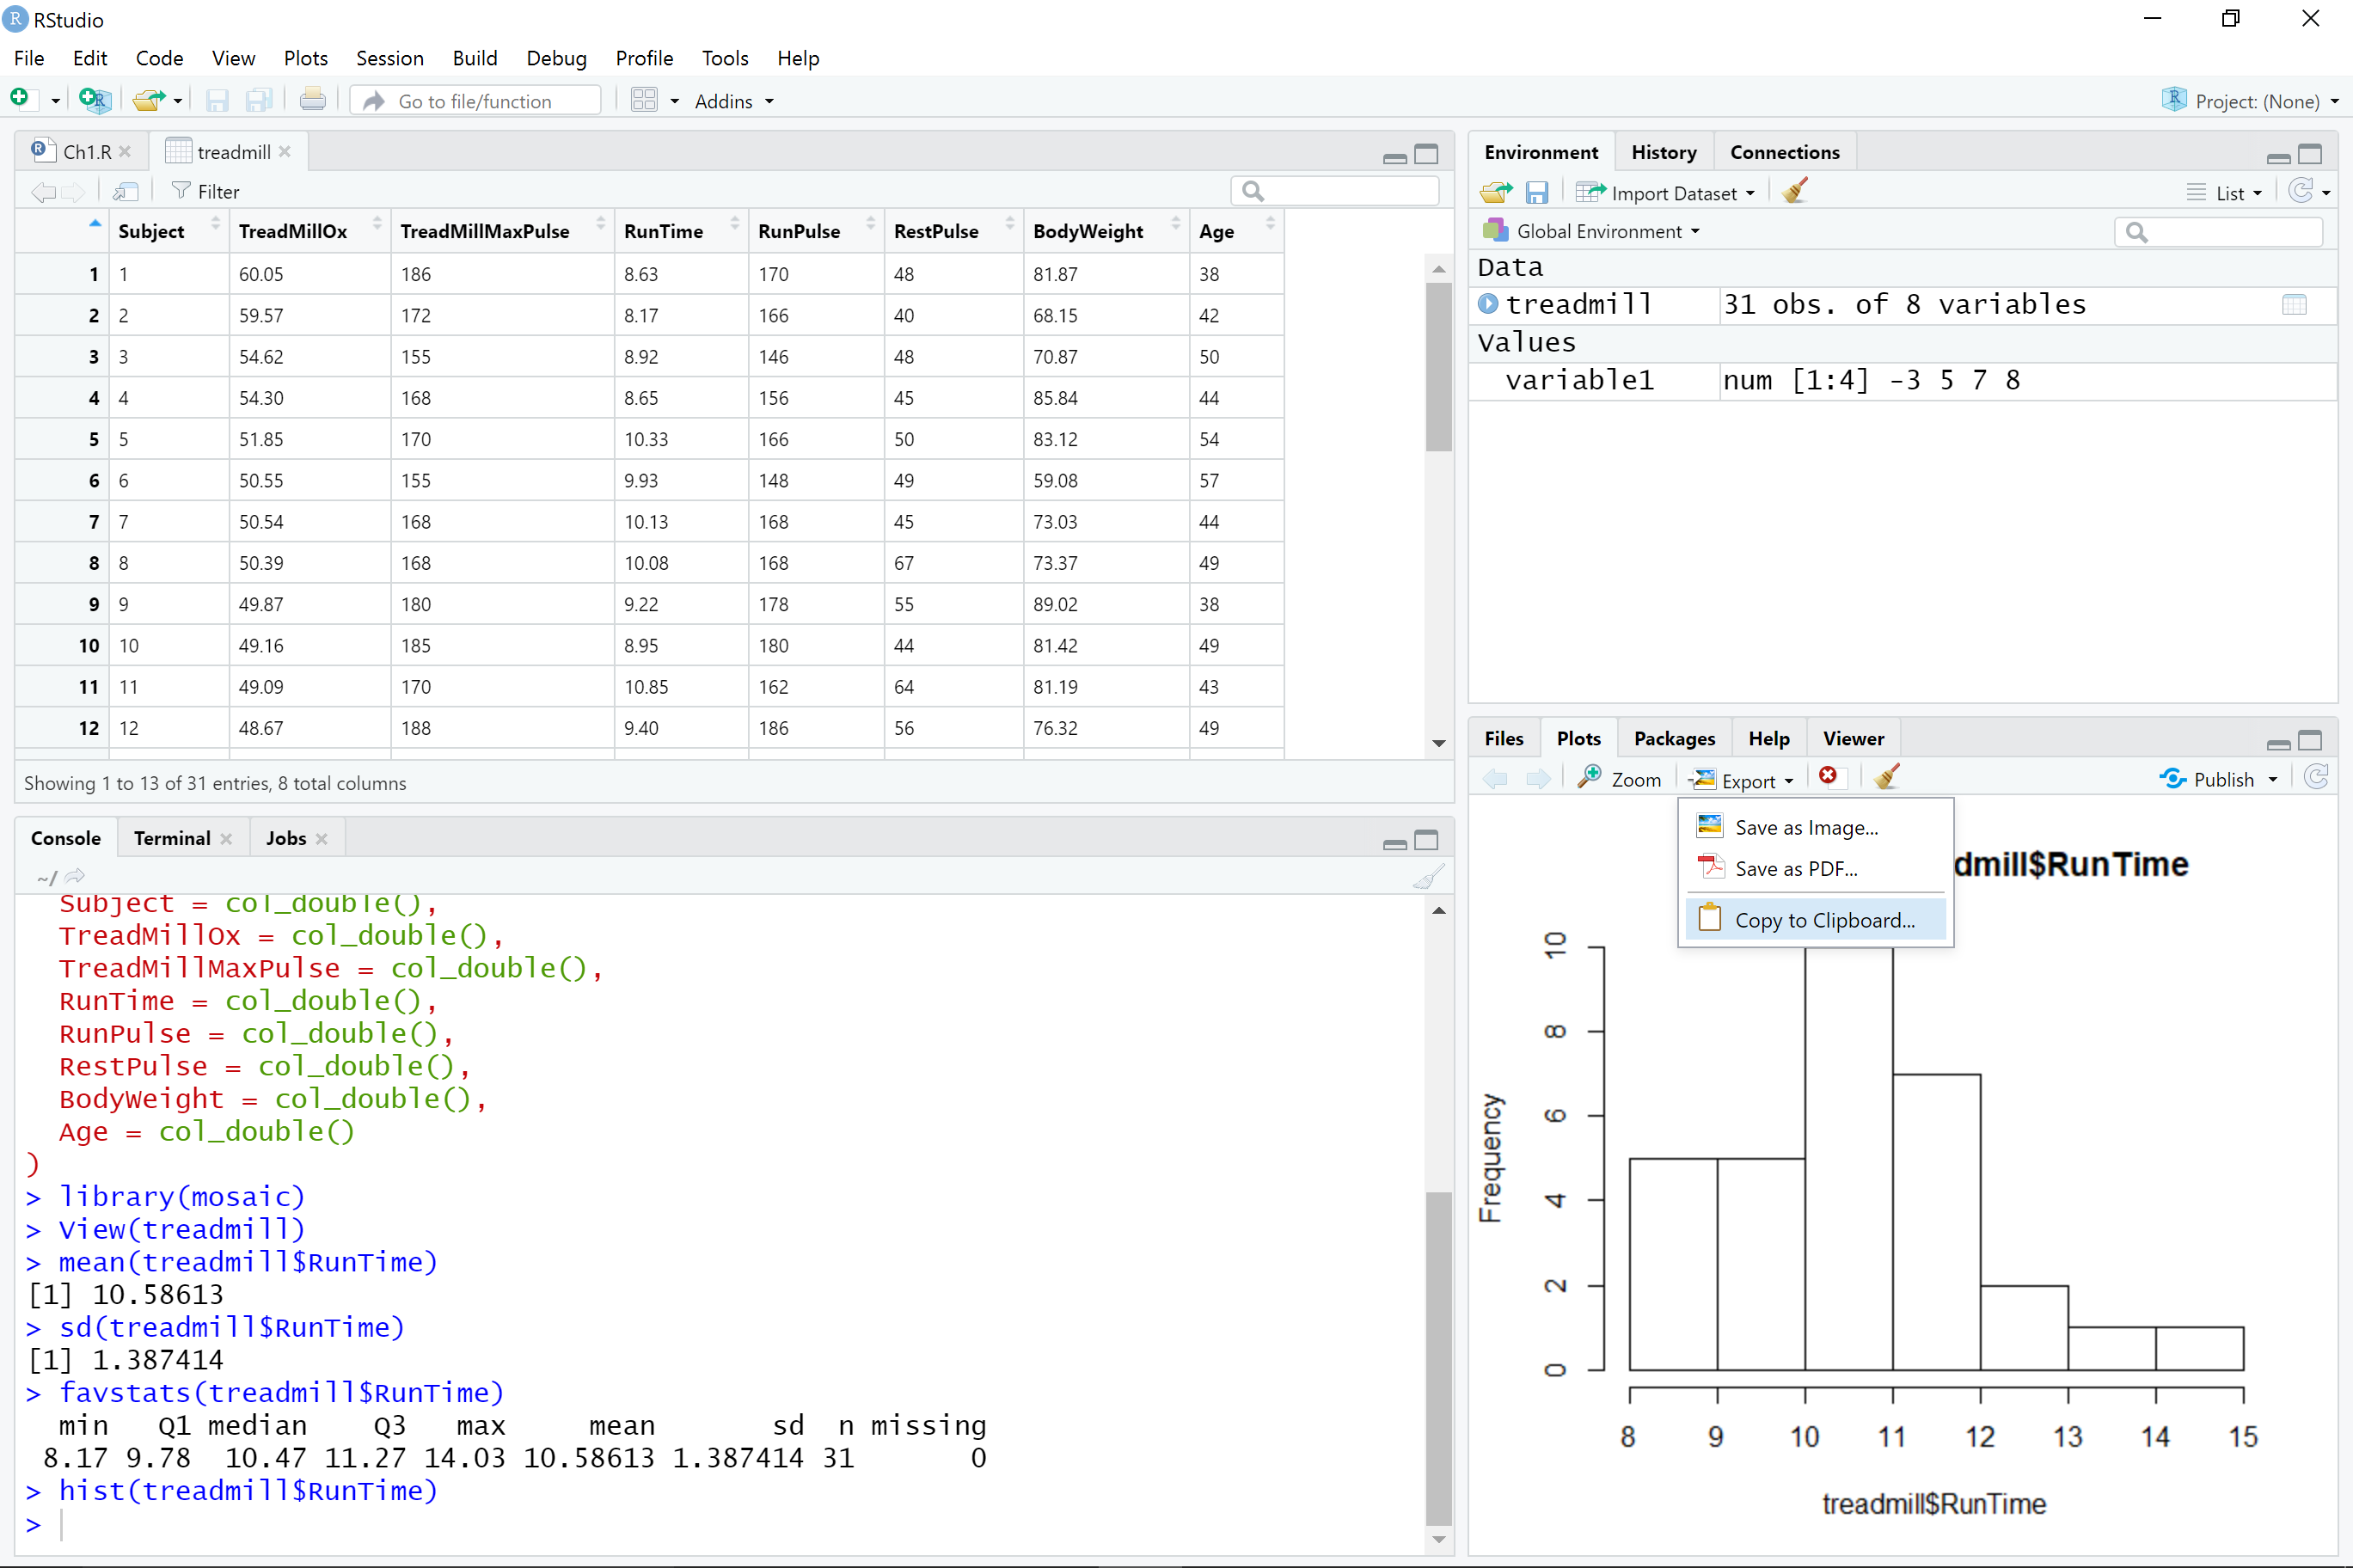
\includegraphics[width=1\linewidth]{chapter1_files/Fig1-6} 

}

\caption{RStudio while in the process of copying the histogram.}\label{fig:Figure1-6}
\end{figure}

\indent You can save this plot by clicking on the \textbf{Export} button found above
the plot, followed by \textbf{Copy to Clipboard} and clicking on the
\textbf{Copy Plot} button. Then if you open your
favorite word-processing program, you should be able to paste it into a
document for writing reports that include the figures. You can see the first
parts of this process in the screen grab in Figure \ref{fig:Figure1-6}. You can also directly save the figures as separate files using
\textbf{Save as Image} or \textbf{Save as PDF} and then insert them into your word
processing documents.

\indent The function \texttt{hist} defaults into providing a histogram on the \textbf{\emph{frequency}}
(count) scale. In most R functions, there are the default options that will
occur if we don't make any specific choices but we
can override the default options if we desire. One option we can modify here is
to add labels to the bars to be able to see exactly how many observations fell
into each bar. Specifically, we can turn the \texttt{labels} option ``on'' by making it true (``T'') by adding \texttt{labels\ =\ T} to the previous call to the \texttt{hist} function, separated by a comma. Note that we will use the \texttt{=} sign only for changing options within functions.

\begin{Shaded}
\begin{Highlighting}[]
\SpecialCharTok{\textgreater{}} \FunctionTok{hist}\NormalTok{(treadmill}\SpecialCharTok{$}\NormalTok{RunTime, }\AttributeTok{labels =}\NormalTok{ T)}
\end{Highlighting}
\end{Shaded}



\begin{figure}[ht!]

{\centering 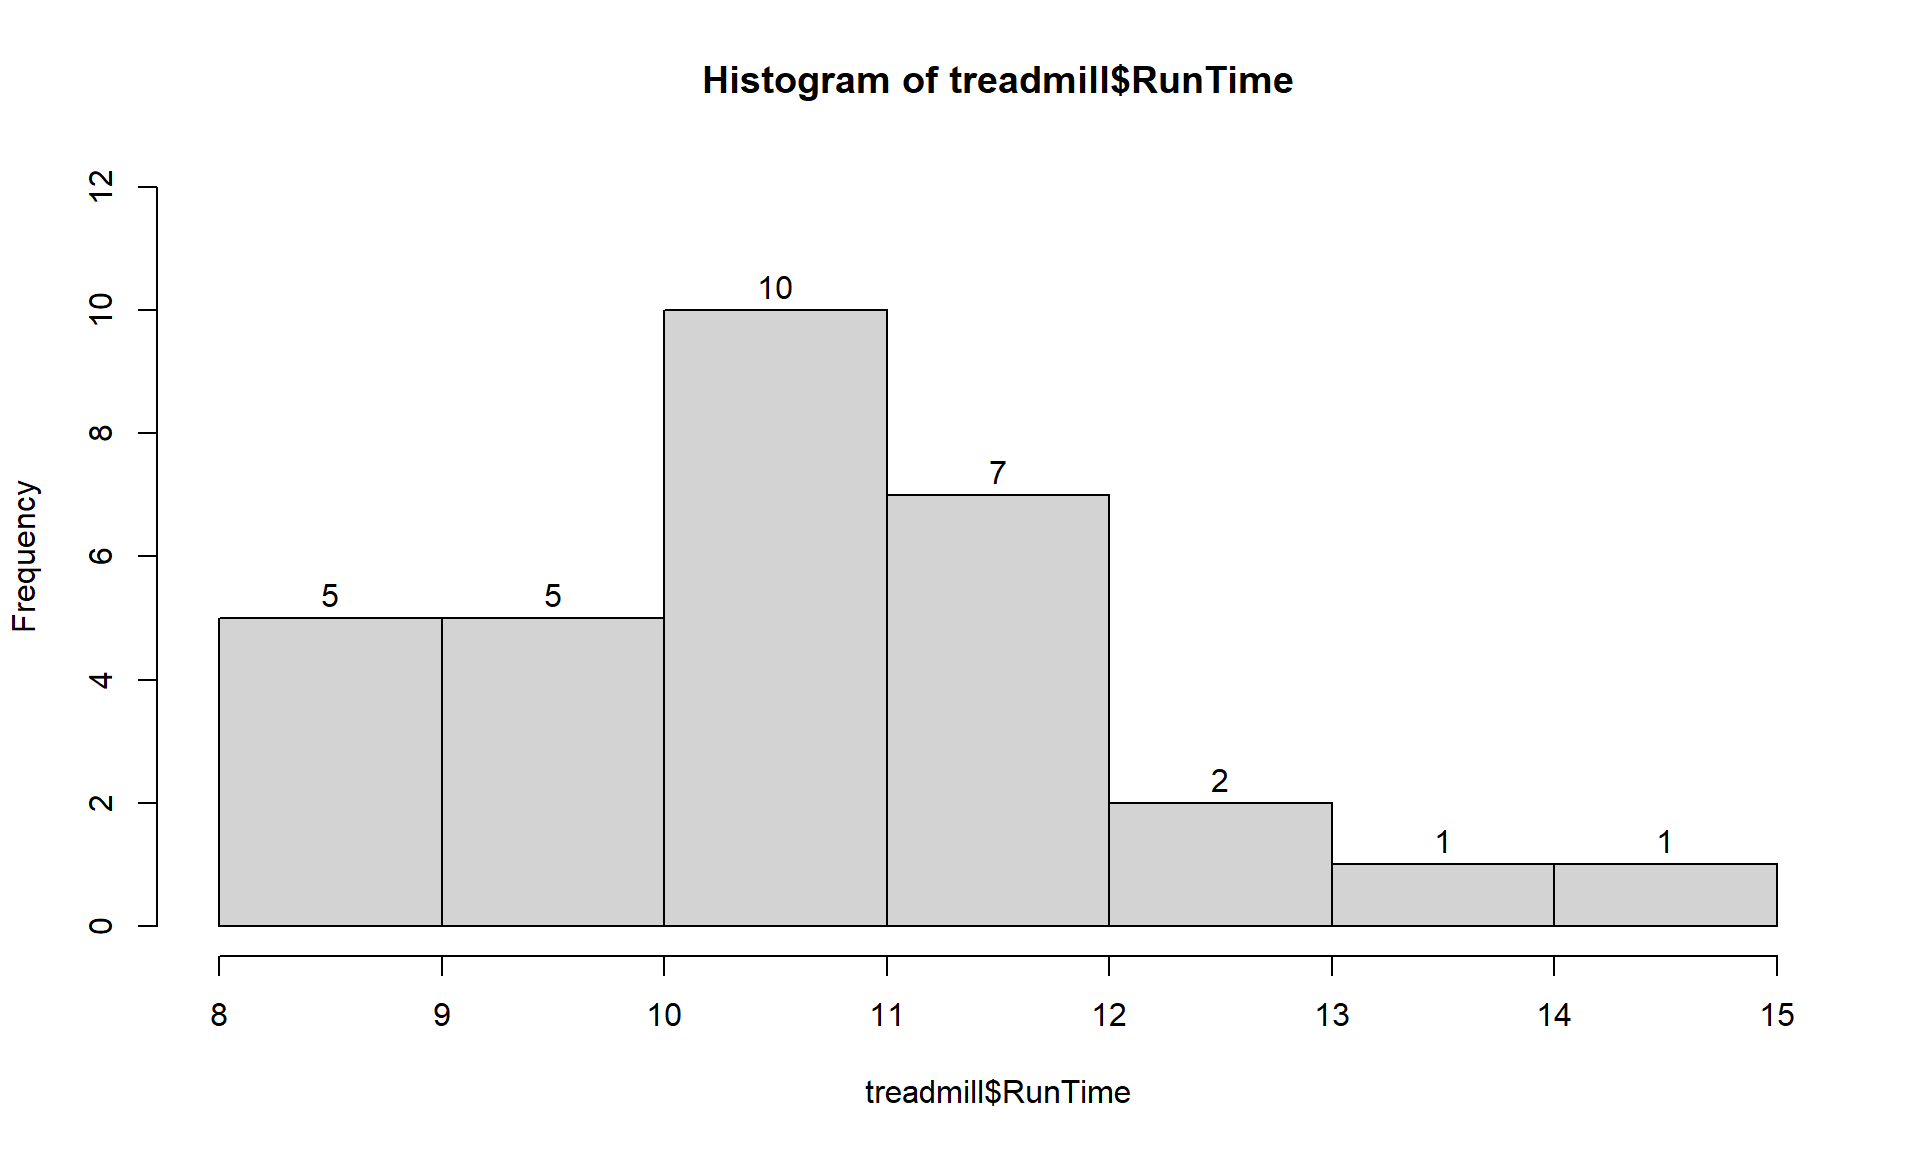
\includegraphics[width=0.75\linewidth]{01-preface_files/figure-latex/Figure1-7-1} 

}

\caption{Histogram of Run Times with counts in bars labeled.}\label{fig:Figure1-7}
\end{figure}

\indent Based on this histogram (Figure \ref{fig:Figure1-8}), it does not appear that there any outliers in the responses
since there are no bars that are separated from the other observations. However,
the distribution does not look symmetric and there might be a skew to the
distribution. Specifically, it appears to be \textbf{\emph{skewed right}} (the right tail is longer than the left). But histograms can sometimes mask features of
the data set by binning observations and it is hard to find the percentiles
accurately from the plot.

\indent When assessing outliers and skew, the \textbf{\emph{boxplot}}
(or \emph{Box and Whiskers} plot) can also be helpful (Figure \ref{fig:Figure1-8}) to describe the
shape of the distribution as it displays the 5-number summary and will also indicate
observations that are ``far'' above the middle of the observations.
\index{boxplot}
R's \texttt{boxplot} function uses the standard rule to indicate an observation as a
\textbf{\emph{potential outlier}} if it falls more than 1.5 times the \textbf{\emph{IQR}}
(Inter-Quartile Range, calculated as Q3 -- Q1) below Q1 or above Q3.
\index{outlier}
The potential outliers
are plotted with circles and the \emph{Whiskers} (lines that extend from Q1 and Q3 typically to
the minimum and maximum) are shortened to only go as far as
observations that are within \(1.5*\)IQR of the upper and lower quartiles. The \emph{box}
part of the boxplot is a box that goes from Q1 to Q3 and the median is displayed as a line
somewhere inside the box.\footnote{The median, quartiles and whiskers sometimes occur at the same
  values when there are many tied observations. If you can't see all the
  components of the boxplot, produce the numerical summary to help you understand
  what happened.} Looking back at the summary statistics above, Q1 = 9.78 and Q3 = 11.27, providing an IQR of:

\begin{Shaded}
\begin{Highlighting}[]
\SpecialCharTok{\textgreater{}}\NormalTok{ IQR }\OtherTok{\textless{}{-}} \FloatTok{11.27} \SpecialCharTok{{-}} \FloatTok{9.78}
\SpecialCharTok{\textgreater{}}\NormalTok{ IQR}
\NormalTok{[}\DecValTok{1}\NormalTok{] }\FloatTok{1.49}
\end{Highlighting}
\end{Shaded}

One observation (the maximum value of 14.03) is indicated as a potential outlier
based on this result by being larger than Q3 \(+1.5*\)IQR, which was 13.505:

\begin{Shaded}
\begin{Highlighting}[]
\SpecialCharTok{\textgreater{}} \FloatTok{11.27} \SpecialCharTok{+} \FloatTok{1.5}\SpecialCharTok{*}\NormalTok{IQR}
\NormalTok{[}\DecValTok{1}\NormalTok{] }\FloatTok{13.505}
\end{Highlighting}
\end{Shaded}

\indent The boxplot also shows a slight indication of a right skew (skew towards
larger values) with the distance from the minimum to the median being smaller than the
distance from the median to the maximum. Additionally, the distance from Q1 to
the median is smaller than the distance from the median to Q3. It is modest skew,
but worth noting.



\begin{figure}[ht!]

{\centering 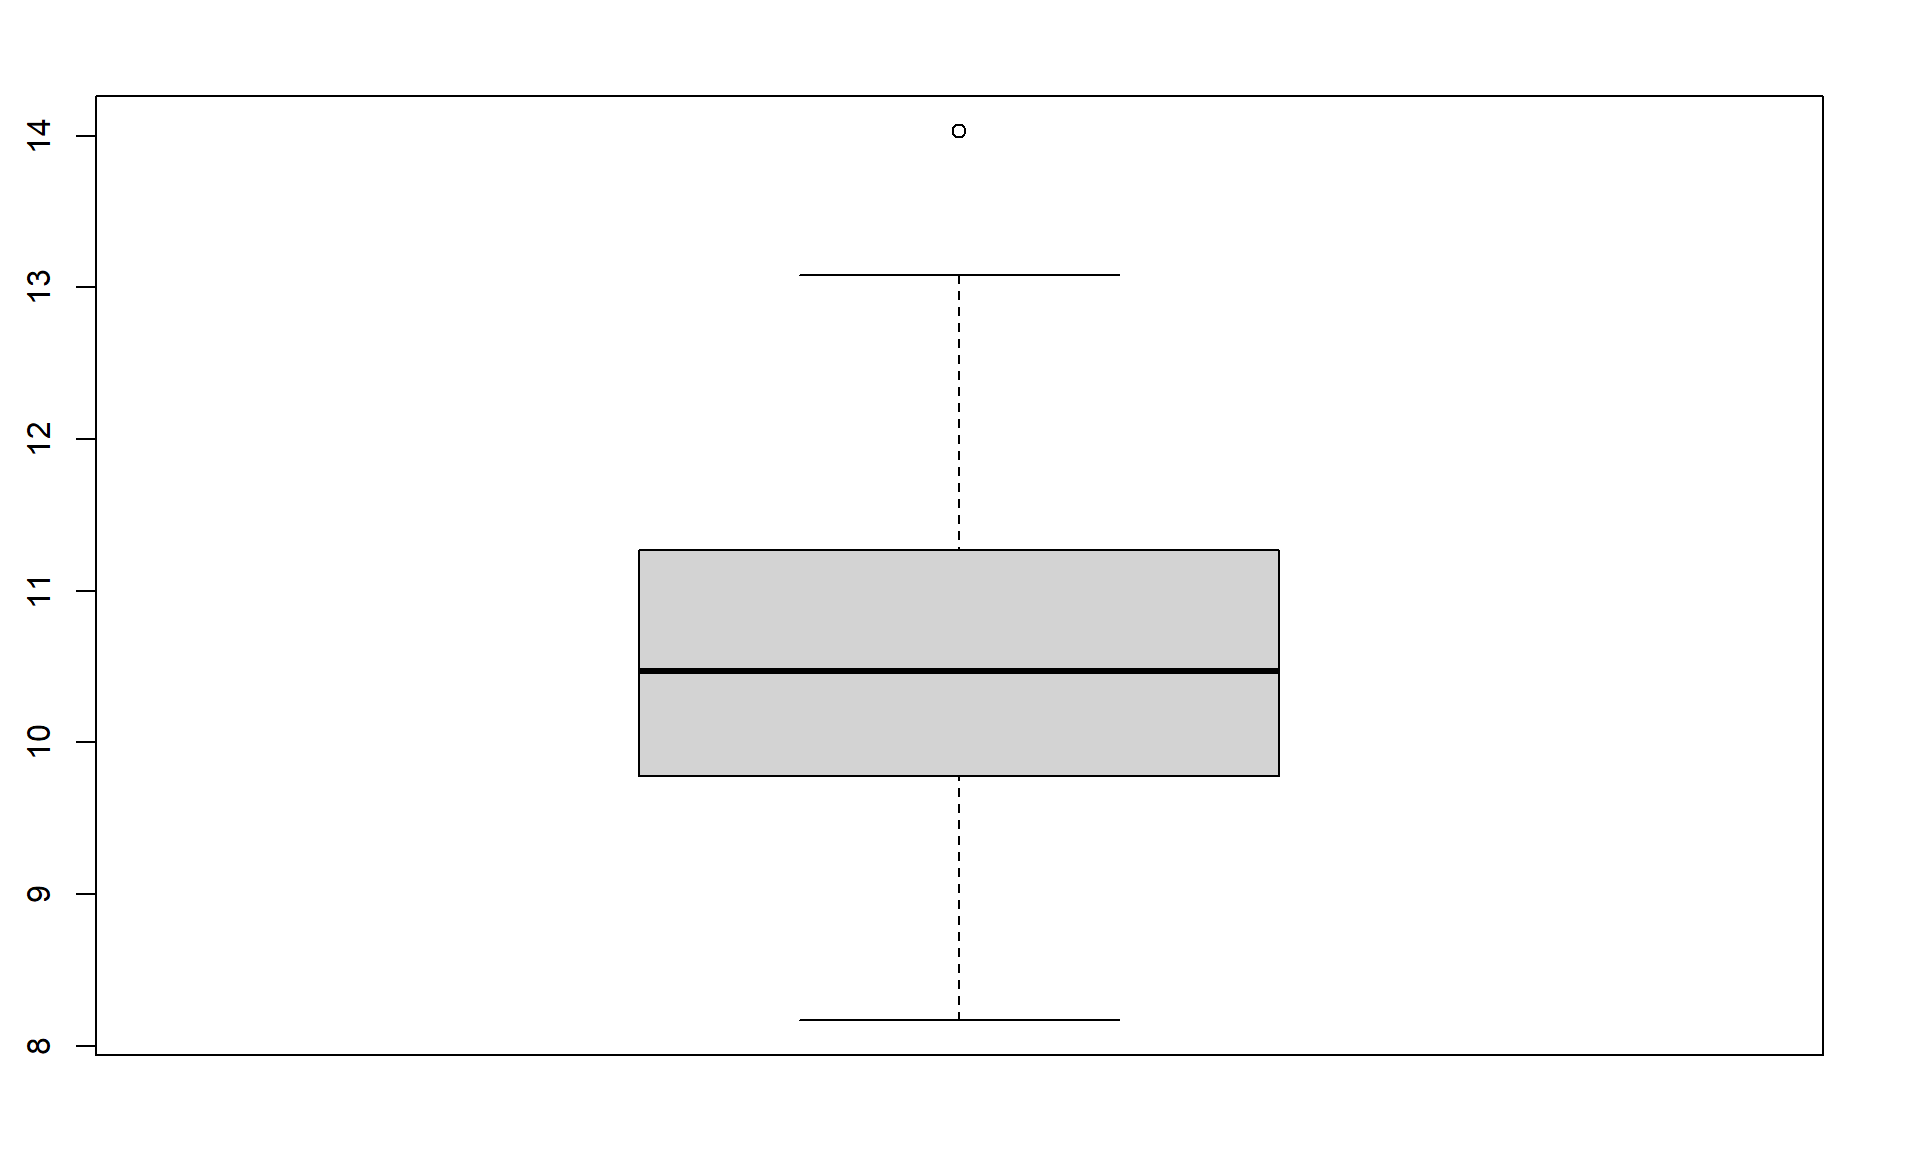
\includegraphics[width=0.75\linewidth]{01-preface_files/figure-latex/Figure1-8-1} 

}

\caption{Boxplot of 1.5 mile Run Times.}\label{fig:Figure1-8}
\end{figure}

\begin{Shaded}
\begin{Highlighting}[]
\SpecialCharTok{\textgreater{}} \FunctionTok{boxplot}\NormalTok{(treadmill}\SpecialCharTok{$}\NormalTok{RunTime)}
\end{Highlighting}
\end{Shaded}

\indent While the default boxplot is fine, it fails to provide good graphical labels,
especially on the y-axis. Additionally, there is no title on the plot. The
following code provides some enhancements to the plot by using the \texttt{ylab} and
\texttt{main} options in the call to \texttt{boxplot}, with the results displayed in
Figure \ref{fig:Figure1-9}. When we add text to plots, it will be contained within quotes and
be assigned into the options \texttt{ylab} (for y-axis) or \texttt{main}
(for the title) here to put it into those locations.



\begin{figure}[ht!]

{\centering 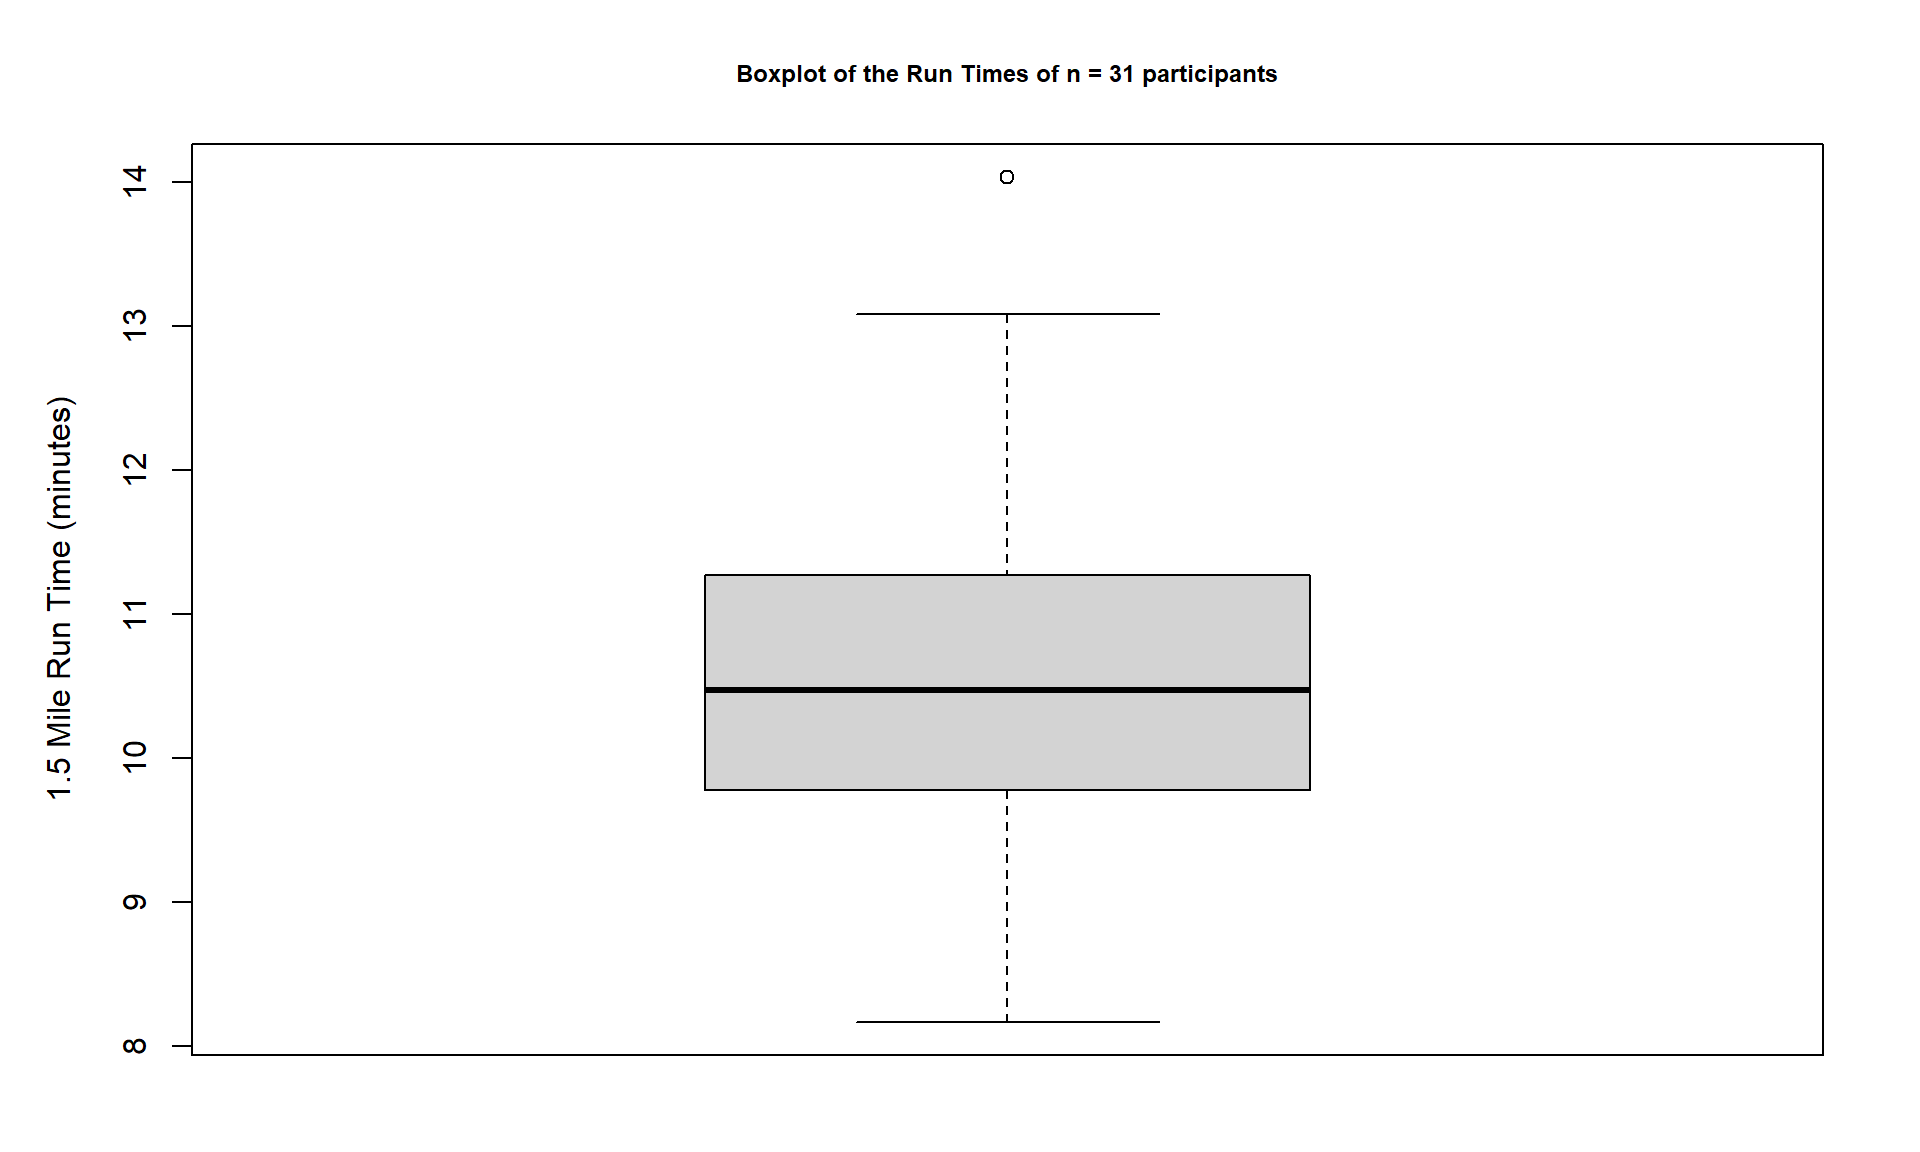
\includegraphics[width=0.75\linewidth]{01-preface_files/figure-latex/Figure1-9-1} 

}

\caption{Boxplot of Run Times with improved labels.}\label{fig:Figure1-9}
\end{figure}

\begin{Shaded}
\begin{Highlighting}[]
\SpecialCharTok{\textgreater{}} \FunctionTok{boxplot}\NormalTok{(treadmill}\SpecialCharTok{$}\NormalTok{RunTime, }\AttributeTok{ylab =} \StringTok{"1.5 Mile Run Time (minutes)"}\NormalTok{, }
          \AttributeTok{main =} \StringTok{"Boxplot of the Run Times of n = 31 participants"}\NormalTok{)}
\end{Highlighting}
\end{Shaded}

\indent Throughout the book, we will often use extra options to make figures that
are easier for you to understand. There
are often simpler versions of the functions that will suffice but the extra
work to get better labeled figures is often worth it. I guess the point is that
``a picture is worth a thousand words'' but in data visualization, that is only
true if the reader can understand what is being displayed. It is also important
to think about the quality of the information that is being displayed,
regardless of how pretty the graphic might be. So maybe it is better to say
``a picture can be worth a thousand words'' if it is well-labeled?

\hypertarget{section1-4}{%
\section{R Markdown}\label{section1-4}}

The previous results were created by running the R code and then copying the
results from either the console or by copying the figure and then pasting the results
into the typesetting program. There is another way
to use RStudio where you can have it compile the results (both output and
figures) directly into a document together with other writing and the code that generated it,
using what is called R Markdown (\url{http://shiny.rstudio.com/articles/rmarkdown.html}).
It is basically what we used to prepare this book and what you should learn to use to do your work.
From here forward, you will see a
change in formatting of the R code and output as you will no
longer see the command prompt (``\textgreater{}'') with the code. The output will be
flagged by having two ``\#\#'''s before it. For example, the summary statistics for
the \emph{RunTime} variable from \texttt{favstats} function would look like when run using R Markdown:

\begin{Shaded}
\begin{Highlighting}[]
\FunctionTok{favstats}\NormalTok{(treadmill}\SpecialCharTok{$}\NormalTok{RunTime)}
\end{Highlighting}
\end{Shaded}

\begin{verbatim}
##   min   Q1 median    Q3   max     mean       sd  n missing
##  8.17 9.78  10.47 11.27 14.03 10.58613 1.387414 31       0
\end{verbatim}

\indent Statisticians (and other scientists) are starting to use R Markdown and
similar methods because they provide what is called ``Reproducible
research'' (\protect\hyperlink{ref-Gandrud2015}{Gandrud 2015}) where all the code and output it produced are
available in a single place. This allows different researchers to run and verify
results (so ``reproducible results'') or the original researchers to revisit their
earlier work at a later date and recreate all their results exactly\footnote{I recently
  had to revisit some work from almost a decade ago (before I switched to using R
  Markdown) as we were working on a journal article submission that re-used some
  of that work and it was unclear where some results came from, so I had to do
  some new work that could have been avoided if I had worked in a reproducible
  fashion.}. Scientific publications are currently
encouraging researchers to work in this way and may someday require it. The
term \textbf{\emph{reproducible}} \index{reproducible} can also be related to whether
repeated studies (with new, independent data collection stages and analyses)
get the same result (also called \textbf{\emph{replication}}) \index{replication} --
further discussion of these terms and the implications for scientific research
are discussed in Chapter \ref{chapter2}.

\indent In order to get some practice using R Markdown, create a sample document
in this format using File -\textgreater{} New File -\textgreater{} R Markdown\ldots{} Choose a title for your
file and select the ``Word'' option. This will create a new file in the upper left
window where we stored our .R script. Save that file to your computer. Then you
can use the ``Knit'' button to have RStudio run the code and create a word
document with the results. R Markdown documents contain basically two
components, ``code chunks'' that contain your code and the rest of the document
where you can write descriptions and interpretations of the results that code
generates. The code chunks can be inserted using the ``Insert'' button by
selecting the ``R'' option. Then write your code in between the
\texttt{\textasciigrave{}\textasciigrave{}\textasciigrave{}\{r\}} and \texttt{\textasciigrave{}\textasciigrave{}\textasciigrave{}} lines (it should have grey highlights for those lines
and white for the rest of the portions of the .Rmd document). Once you write
some code inside a code chunk, you can test your code using the triangle on the
upper right side of it to run all the code that resides in that chunk. Keep your
write up outside of these code chunks to avoid code errors and failures to
compile. Once you think your code and writing is done, you can use the ``Knit''
button to try to compile the file. As you are learning, you may find this
challenging, so start with trying to review the sample document and knit each
time you get a line of code written so you know which line was responsible for
preventing the knitting from being successful. Also look around for posted
examples of .Rmd files to learn how others have incorporated code with
write-ups. You might even be given a template of homework or projects as .Rmd
files from your instructor. After you do this a couple of times, you will find
that the challenge of working with markdown files is more than matched by the
simplicity of the final product and, at least to researchers, the
reproducibility and documentation of work that this way of working provides.

\hypertarget{section1-5}{%
\section{Grammar of Graphics}\label{section1-5}}

The previous plots were made using what is called ``base R'' graphics. It is
possible to make versions of all the graphics we need in this material using
single function calls like \texttt{boxplot} -- and there are some places we will
utilize these simple versions because they get us exactly what we want to see.
But to make more complex displays and have complete control of the way the
graphs look, we will utilize the \texttt{ggplot2} package (\protect\hyperlink{ref-R-ggplot2}{Wickham et al. 2022}) which was
built to implement a type of grammar for making and layering graphical displays
of data, adding each layer step by step. \index{\texttt{ggplot}}
\index{R packages!\textbf{ggplot2}} While it takes a little bit of work to get
started, the power of these displays will ultimately make the investment
worthwhile\footnote{This discussion is based on materials developed for a data
  visualization workshop originally developed by Dr.~Allison Theobold and related
  to the \url{https://datacarpentry.org/} workshops.}.

\indent As opposed to base graphics, the ggplots will contain multiple components
that are patched together with a \texttt{+}, with the general format of
\texttt{ggplot(data\ =\ \textless{}DATA\textgreater{},\ mapping\ =\ aes(\textless{}VARIABLE\ MAPPINGS\textgreater{}))\ +\ \textless{}GEOM\_FUNCTION\textgreater{}()}.
Breaking this down, the \texttt{data\ =\ ...} tells the \texttt{ggplot} function where to look,
the information inside the \texttt{aes} (or aesthetic) defines which variables in the
data set to use and how to use them (often with \texttt{x\ =\ variable1},
\texttt{y\ =\ variable2}, etc., with \texttt{x\ =\ ...} for the variable on the x (horizontal)
axis and \texttt{y\ =\ ...} for the variable on the y (vertical) axis), and the
\texttt{+\ \textless{}GEOM\_FUNCTION\textgreater{}()} defines which type of graph to make (there are
\texttt{geom\_histogram} and \texttt{geom\_boxplot} to make the graphs discussed previously and
many, many more). Because we often have many ``+'''s to include, the common
practice is to hit return after the ``+'' and start the next layer or option on
the following line for better readability. Figure \ref{fig:Figure1-10} shows a
histogram of the \texttt{RunTime} variable made using the \texttt{+\ geom\_histogram()}.
\index{\texttt{geom\_histogram}} \index{\texttt{geom\_boxplot}}



\begin{Shaded}
\begin{Highlighting}[]
\FunctionTok{library}\NormalTok{(ggplot2)}
\FunctionTok{ggplot}\NormalTok{(}\AttributeTok{data =}\NormalTok{ treadmill, }\AttributeTok{mapping =} \FunctionTok{aes}\NormalTok{(}\AttributeTok{x =}\NormalTok{ RunTime)) }\SpecialCharTok{+} \FunctionTok{geom\_histogram}\NormalTok{()}
\end{Highlighting}
\end{Shaded}

\begin{verbatim}
`stat_bin()` using `bins = 30`. Pick better value with `binwidth`.
\end{verbatim}

\begin{figure}[ht!]

{\centering 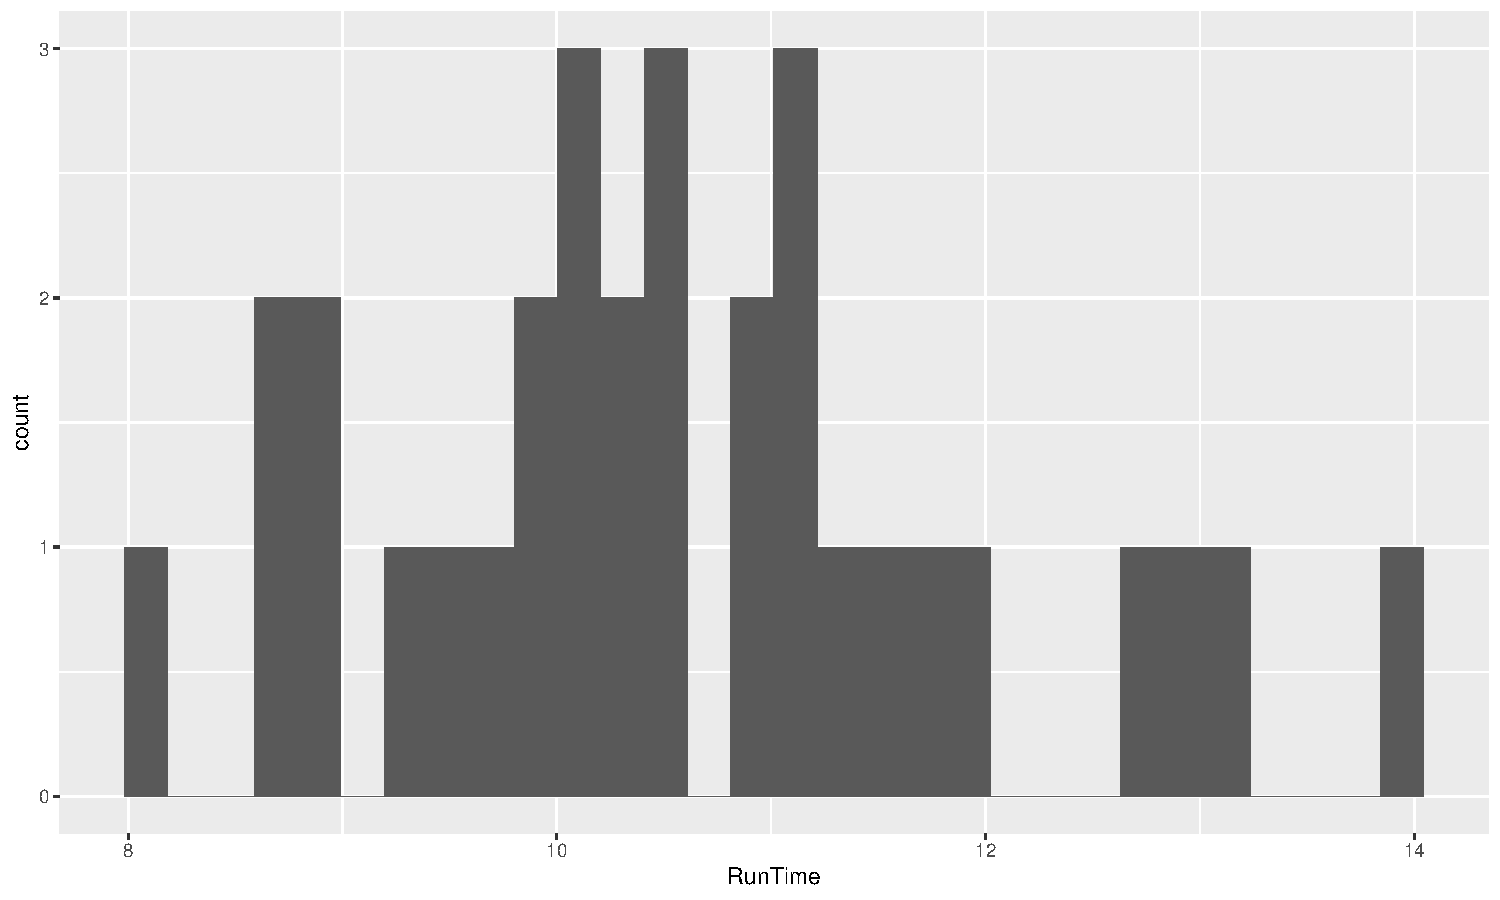
\includegraphics[width=0.75\linewidth]{01-preface_files/figure-latex/Figure1-10-1} 

}

\caption{Default histogram of Run Times using \texttt{ggplot}.}\label{fig:Figure1-10}
\end{figure}

\newpage

The warning message reflects a challenge in making histograms that involves how
many bins to use. In \texttt{geom\_histogram}, it always uses 30 bins and expects you to
make your own choice, compared to \texttt{hist} that used a different method to try to
make a better automatic choice, but there is no single right answer. So maybe we
should try out other values to get a ``smoother'' result here, which we can do by
adding the \texttt{bins\ =\ ...} to the \texttt{+\ geom\_histogram()}, such as
\texttt{+\ geom\_histogram(bins\ =\ 8)} to get an 8 bin histogram in
Figure \ref{fig:Figure1-11}.



\begin{figure}[ht!]

{\centering 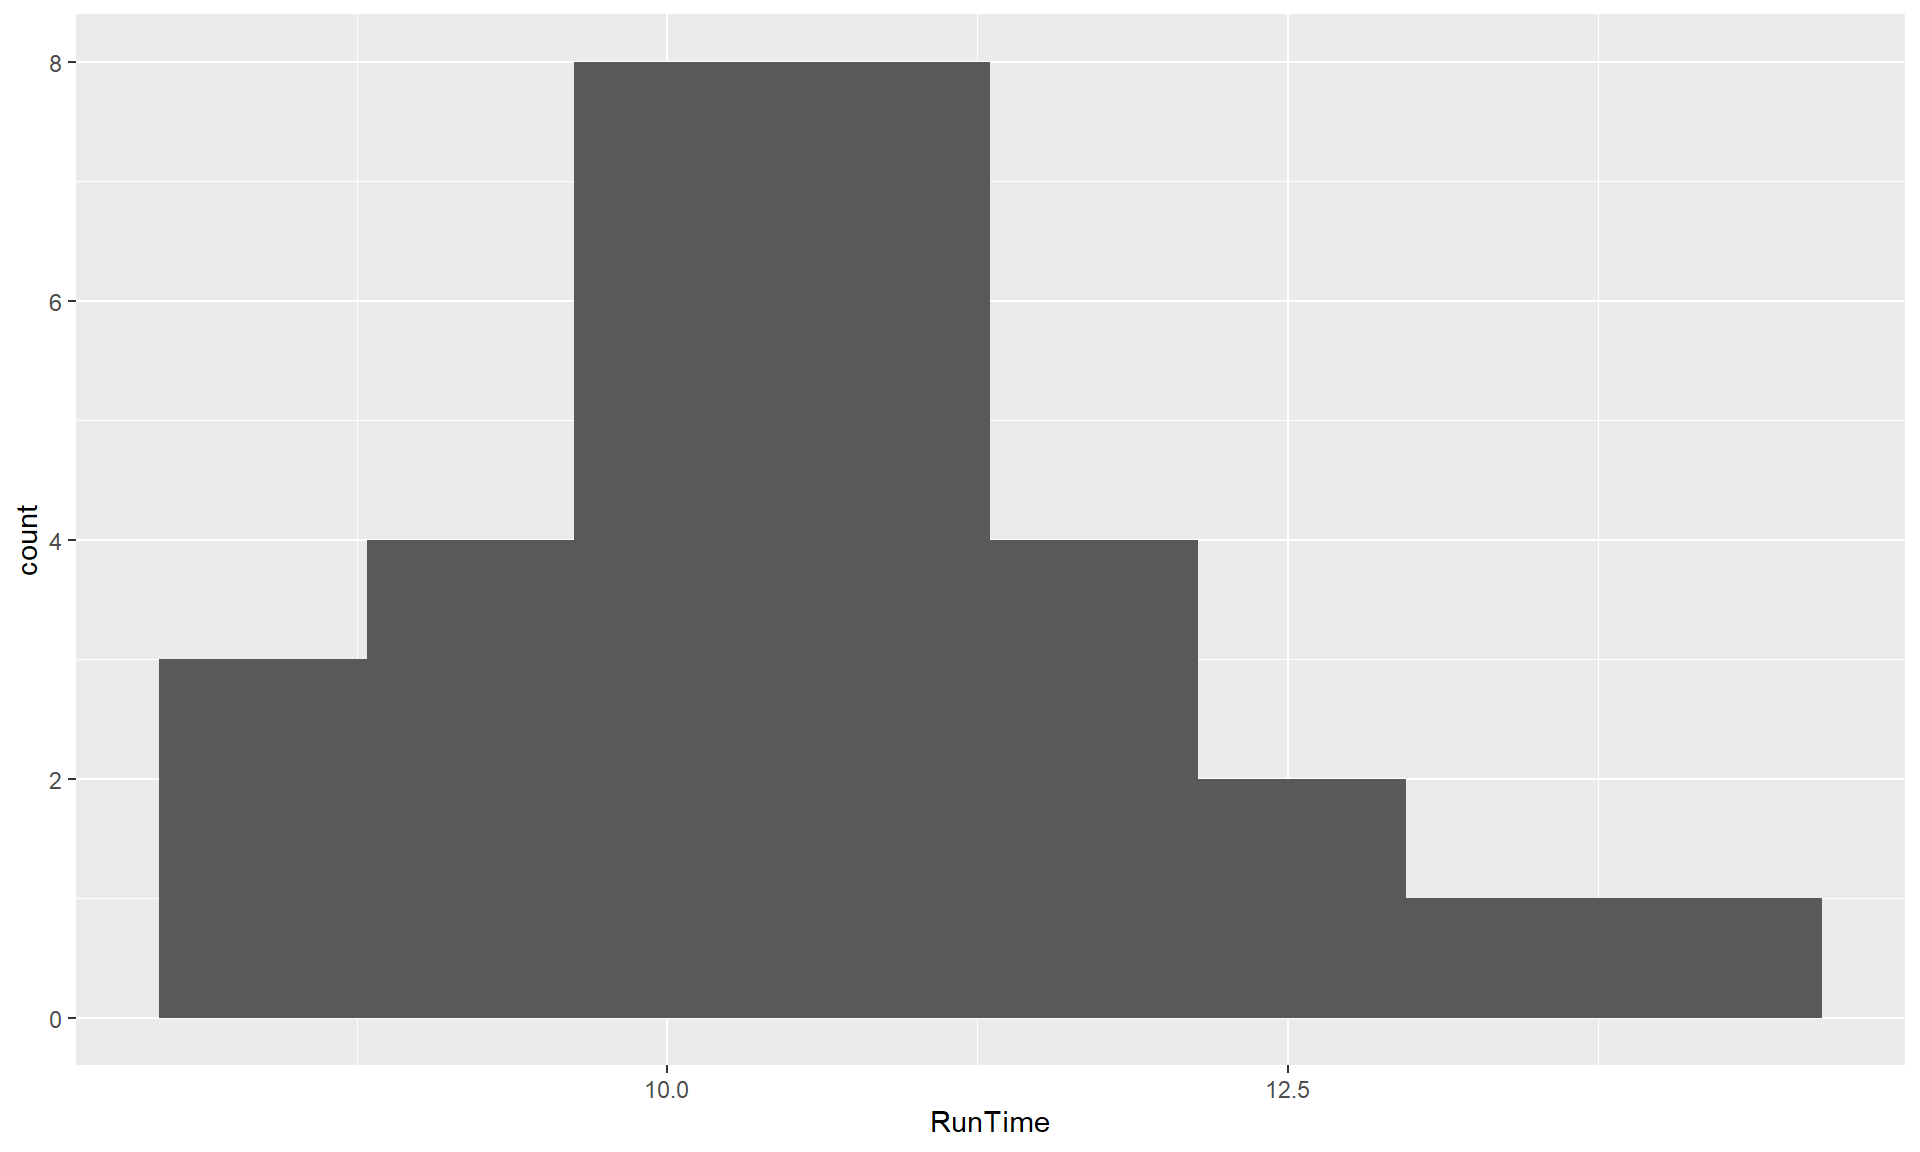
\includegraphics[width=0.75\linewidth]{01-preface_files/figure-latex/Figure1-11-1} 

}

\caption{Histogram of Run Times using \texttt{ggplot} with 8 bins.}\label{fig:Figure1-11}
\end{figure}

\begin{Shaded}
\begin{Highlighting}[]
\FunctionTok{ggplot}\NormalTok{(}\AttributeTok{data =}\NormalTok{ treadmill, }\AttributeTok{mapping =} \FunctionTok{aes}\NormalTok{(}\AttributeTok{x =}\NormalTok{ RunTime)) }\SpecialCharTok{+} 
  \FunctionTok{geom\_histogram}\NormalTok{(}\AttributeTok{bins =} \DecValTok{8}\NormalTok{)}
\end{Highlighting}
\end{Shaded}

\newpage

\indent The following chapters will explore further modifications for these
plots, but there are a couple of additions to highlight. The first is that we
can often layer multiple geoms on the same plot and the order of the additions
defines which layer is ``on top'', with the plot built up sequentially. So we can
add a boxplot on top of a histogram by putting it after the histogram layer.
Also in Figure \ref{fig:Figure1-12}, the \texttt{geom\_rug} is also added, which puts
a tick mark for each observation on the lower part of the x-axis. \index{rug}
Rug plots can also use a graphical technique called \textbf{\emph{jittering}} to add a little
noise using the options \texttt{geom\_rug(sides\ =\ "b",\ aes(y\ =\ 0),\ position\ =\ "jitter")}\footnote{Jittering typically involves adding random variability to each
  observation that is uniformly distributed in a range determined based on the
  spacing of the observations. The idea is to jitter just enough to see all the
  points but not too much. Because it is random noise being added, this also means that if you re-run the \texttt{jitter} function,
  the results will change if you do not set the random number seed using
  \texttt{set.seed} that is discussed more below. For more details, type \texttt{help(geom\_rug)}
  in the console in RStudio. The code is unfortunately clumsy to add jittering to the rug, so a simpler option is to use \texttt{geom\_rug(alpha\ =\ 0.3)} where the transparency is modified with the \texttt{alpha} option to help with identifying overplotting of lines in the rug.} to each observation so that multiple similar or
tied observations do not plot as a single line. \index{jitter} There are options
to control the color of individual components when we add them (the histogram is
filled with grey (\texttt{fill\ =\ "grey"}), the boxplot is in ``tomato''
(\texttt{color\ =\ "tomato"}), and the rug plot is in ``skyblue''). Finally, the last
change here is to the ``theme'' for the plot\footnote{This certainly could have waited
  until later, but I have now seen enough base ggplot graphs that I really like
  to change their overall look.} which we can include one of a suite of different
layouts with themes such as \texttt{+\ theme\_bw()} or \texttt{+\ theme\_light()}. If you add the
\texttt{ggthemes} package(\protect\hyperlink{ref-R-ggthemes}{Arnold 2021}), you can access a long list of alternative looks
for your plot (see \url{https://jrnold.github.io/ggthemes/reference/index.html} for
options there). \index{themes} \index{\texttt{theme\_bw()}}
\index{\texttt{geom\_rug()}}



\begin{figure}[ht!]

{\centering 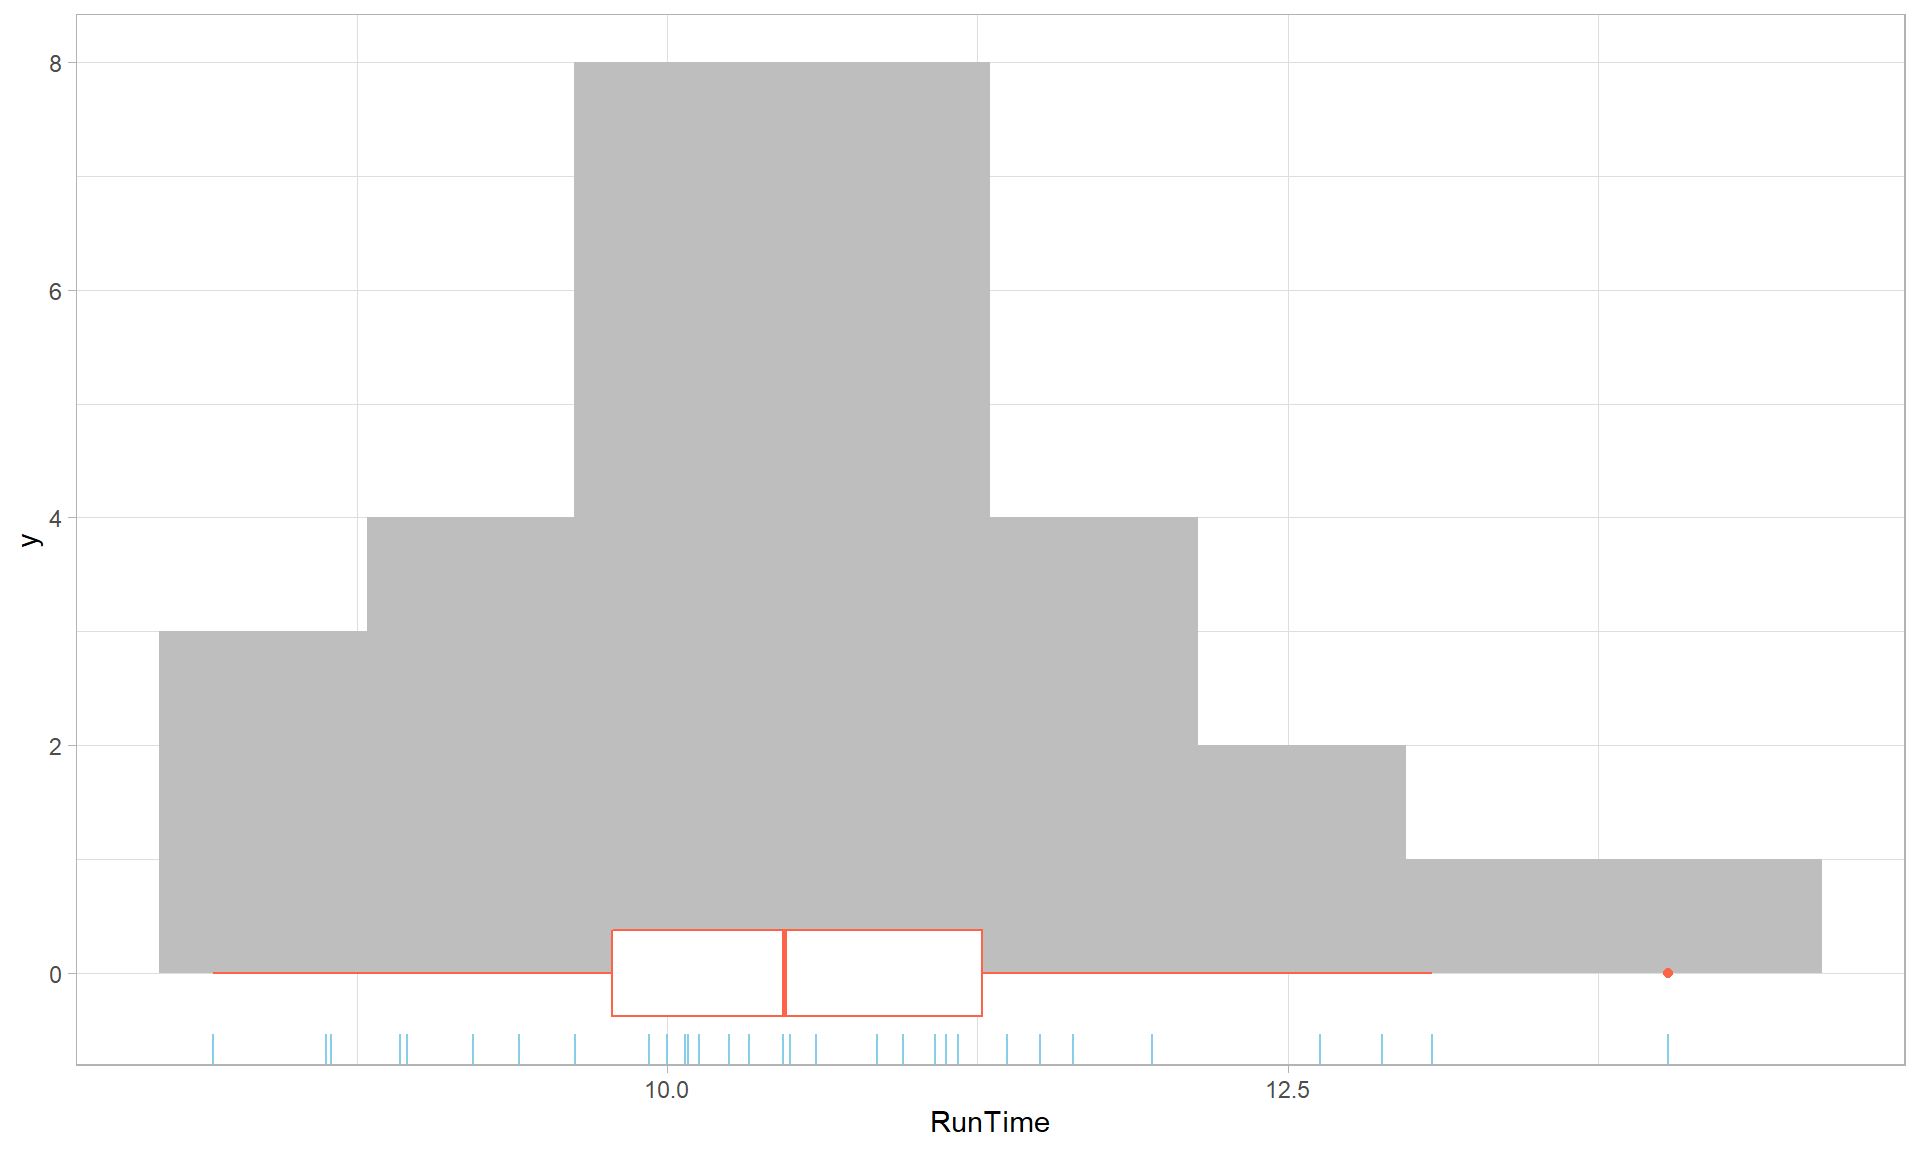
\includegraphics[width=0.75\linewidth]{01-preface_files/figure-latex/Figure1-12-1} 

}

\caption{Histogram with boxplot and rug of Run Times using \texttt{ggplot} with modified colors and theme.}\label{fig:Figure1-12}
\end{figure}

\begin{Shaded}
\begin{Highlighting}[]
\FunctionTok{ggplot}\NormalTok{(}\AttributeTok{data =}\NormalTok{ treadmill, }\AttributeTok{mapping =} \FunctionTok{aes}\NormalTok{(}\AttributeTok{x =}\NormalTok{ RunTime)) }\SpecialCharTok{+} 
  \FunctionTok{geom\_histogram}\NormalTok{(}\AttributeTok{fill =} \StringTok{"grey"}\NormalTok{, }\AttributeTok{bins =} \DecValTok{8}\NormalTok{) }\SpecialCharTok{+} 
  \FunctionTok{geom\_boxplot}\NormalTok{(}\AttributeTok{color =} \StringTok{"tomato"}\NormalTok{) }\SpecialCharTok{+} 
    \FunctionTok{geom\_rug}\NormalTok{(}\AttributeTok{color =} \StringTok{"skyblue"}\NormalTok{, }\AttributeTok{sides =} \StringTok{"b"}\NormalTok{, }\FunctionTok{aes}\NormalTok{(}\AttributeTok{y =} \DecValTok{0}\NormalTok{), }\AttributeTok{position =} \StringTok{"jitter"}\NormalTok{) }\SpecialCharTok{+} 
  \FunctionTok{theme\_light}\NormalTok{()}
\end{Highlighting}
\end{Shaded}

\newpage

\hypertarget{section1-6}{%
\section{Exiting RStudio}\label{section1-6}}

Finally, when you are done with your work and attempt to exit out of RStudio,
it will ask you to save your workspace. \textbf{\emph{DO NOT DO THIS!}} It will just
create a cluttered workspace and could even cause you to get incorrect results.

\indent In fact, you should go into the Tools -\textgreater{} Global Options and then make sure that
``Save workspace to .RData on exit'' option on the first screen you will see is
set to \textbf{\emph{Never}}. If you save your R code either as a .R or (better) an R
Markdown (.Rmd) file, you can re-create any results by simply
re-running that code or re-knitting the file. If you find that you have lots of
``stuff'' in your workspace because you accidentally saved your workspace, just
run \texttt{rm(list\ =\ ls())}. It will delete all the data sets from your workspace.

\hypertarget{section1-7}{%
\section{Chapter summary}\label{section1-7}}

This chapter covered getting R and RStudio downloaded and some basics of working with
R via RStudio. You should be able to read a data set into R and run some basic
functions, all done using the RStudio interface. If you are struggling with
this, you should seek additional help with these technical issues so that you
are ready for more complicated statistical methods that are going to be
encountered in the following chapters. The way everyone learns R is
by starting with some example code that does most of what you want to do and
then you modify it. If you can complete the Practice Problems that follow, you
are well on your way to learning to use R.

\indent The statistical methods in this chapter were minimal and all should have been
review. They involved a quick reminder of summarizing the center, spread, and
shape of distributions using numerical summaries of the mean and SD and/or the
min, Q1, median, Q3, and max and the histogram and boxplot as graphical
summaries. We revisited the ideas of symmetry and skew. But the main point was
really to get a start on using R via RStudio to provide results you should be familiar with
from your previous statistics experience(s) and to introduce some of the code we
will be building on in the next chapters.

\newpage

\hypertarget{section1-8}{%
\section{Summary of important R code}\label{section1-8}}

To help you learn and use R, there is a section highlighting the most important
R code used near the end of each
chapter. The bold text will never change but the
lighter and/or ALL CAPS text (red in the online or digital version) will need
to be customized to your particular application. The sub-bullet for each
function will discuss the use of the function and pertinent options or packages
required. You can use this as a guide to finding the function names and some
hints about options that will help you to get the code to work. You can also
revisit the worked examples using each of the functions.

\begin{itemize}
\item
  \textcolor{red}{FILENAME} \texttt{\textless{}-} \textbf{read\_csv(}\textcolor{red}{"path to csv file/FILENAME.csv"}\textbf{)}

  \begin{itemize}
  \item
    Can be generated using ``Import Dataset'' button or by modifying this text.
  \item
    Requires the \texttt{readr} package to be loaded (\texttt{library(readr)}) when using
    the code directly.
  \item
    Imports a text file saved in the CSV format.
  \end{itemize}
\item
  \textcolor{red}{DATASETNAME}\textbf{\$}\textcolor{red}{VARIABLENAME}

  \begin{itemize}
  \tightlist
  \item
    To access a particular variable in a tibble called DATASETNAME, use
    a \$ and then the VARIABLENAME.
  \end{itemize}
\item
  \textbf{head(}\textcolor{red}{DATASETNAME}\textbf{)}

  \begin{itemize}
  \tightlist
  \item
    Provides a list of the first few rows of the data set for all the
    variables in it. \index{\texttt{head()}|textbf}
  \end{itemize}
\item
  \textbf{tail(}\textcolor{red}{DATASETNAME}\textbf{)}

  \begin{itemize}
  \tightlist
  \item
    Provides a list of the last few rows of the data set for all the
    variables in it. \index{\texttt{tail()}|textbf}
  \end{itemize}
\item
  \textbf{mean(}\textcolor{red}{DATASETNAME}\textbf{\$}\textcolor{red}{VARIABLENAME}\textbf{)}

  \begin{itemize}
  \tightlist
  \item
    Calculates the mean of the observations in a variable.
    \index{\texttt{mean()}|textbf}
  \end{itemize}
\item
  \textbf{sd(}\textcolor{red}{DATASETNAME}\textbf{\$}\textcolor{red}{VARIABLENAME}\textbf{)}

  \begin{itemize}
  \tightlist
  \item
    Calculates the standard deviation of the observations in a variable.
    \index{\texttt{sd()}|textbf}
  \end{itemize}
\item
  \textbf{favstats(}\textcolor{red}{DATASETNAME}\$\textcolor{red}{VARIABLENAME}\textbf{)}

  \begin{itemize}
  \item
    Requires the \texttt{mosaic} package to be loaded (\texttt{library(mosaic)}) after
    installing the package).
  \item
    Provides a suite of numerical summaries of the observations in a variable.
    \index{\texttt{favstats()}|textbf}
  \end{itemize}
\item
  \textbf{hist(}\textcolor{red}{DATASETNAME}\textbf{\$}\textcolor{red}{VARIABLENAME}\textbf{)}

  \begin{itemize}
  \tightlist
  \item
    Makes a histogram. \index{\texttt{hist()}|textbf}
  \end{itemize}
\item
  \textbf{boxplot(}\textcolor{red}{DATASETNAME}\textbf{\$}\textcolor{red}{VARIABLENAME}\textbf{)}

  \begin{itemize}
  \tightlist
  \item
    Makes a boxplot. \index{\texttt{boxplot()}|textbf}
  \end{itemize}
\item
  \textbf{ggplot(data = }\textcolor{red}{DATASETNAME}\textbf{, mapping = aes(}\textcolor{red}{VARIABLENAME}\textbf{)) +\\
  geom\_histogram(bins = }\textcolor{red}{10}\textbf{)}

  \begin{itemize}
  \tightlist
  \item
    Makes a histogram with 10 bins using \texttt{ggplot}, requires the \texttt{ggplot2}
    library is installed and loaded. \index{\texttt{geom\_histogram()}|textbf}
  \end{itemize}
\end{itemize}

\newpage

\hypertarget{section1-9}{%
\section{Practice problems}\label{section1-9}}

In each chapter, the last section contains some questions for you to complete
to make sure you understood the
material. You can download the code to answer questions 1.1 to 1.5 below at
\url{http://www.math.montana.edu/courses/s217/documents/Ch1.Rmd}. But to practice
learning R, it would be most useful for you to try to accomplish the requested tasks
yourself and then only refer to the provided R code if/when you struggle.
These questions provide a great venue to check your learning, often to see the
methods applied to another data set, and for something to discuss in study groups,
with your instructor, and at the Math Learning Center.

1.1. Open RStudio and go to File -\textgreater{} New File -\textgreater{} R Markdown\ldots{} to create a .Rmd.
Click on the ``Knit'' button and see what happens. Try to complete the following
questions in that document, clicking on the Knit button after you add a code
chunk with code to complete each question. Part of the assignment on this
question is to not get frustrated the first time you are trying this and seek
out help to answer questions you have when practicing.

1.2. Read in the treadmill data set
discussed previously and find the mean and SD of the Ages (\texttt{Age} variable) and Body
Weights (\texttt{BodyWeight} variable). In studies involving human subjects, it is
common to report a
summary of characteristics of the subjects. Why does this matter? Think about
how your interpretation of any study of the fitness of subjects would change if
the mean age (same spread) had been 20 years older or 35 years younger.

1.3. How does knowing about the
distribution of results for \emph{Age} and \emph{BodyWeight} help you understand the
results for the Run Times discussed previously?

1.4. The mean and SD are most useful
as summary statistics only if the distribution is relatively symmetric. Make a
histogram of \emph{Age} responses and
discuss the shape of the distribution (is it skewed right, skewed left,
approximately symmetric?; are there outliers?). Approximately what range of
ages does this study pertain to?

1.5. The weight responses are in
kilograms and you might prefer to see them in pounds. The conversion is
\texttt{lbs\ =\ 2.205*kgs}. Create a new variable in the \texttt{treadmill}
tibble called \emph{BWlb} using this code:

\begin{Shaded}
\begin{Highlighting}[]
\NormalTok{treadmill}\SpecialCharTok{$}\NormalTok{BWlb }\OtherTok{\textless{}{-}} \FloatTok{2.205}\SpecialCharTok{*}\NormalTok{treadmill}\SpecialCharTok{$}\NormalTok{BodyWeight}
\end{Highlighting}
\end{Shaded}

and find the mean and SD of the new variable (\emph{BWlb}).

1.6. Make histograms and boxplots of
the original \emph{BodyWeight} and new \emph{BWlb} variables, both using base R plots and
using \texttt{ggplot2}. Discuss aspects of the
distributions that changed and those that remained the same with the
transformation from kilograms to pounds. What does this tell you about changing
the units of a variable in terms of its distribution?

\hypertarget{chapter2}{%
\chapter{Linear Models: A Review}\label{chapter2}}

This book is not intended to be a first experience with regression model building, but instead to add to previous experiences with this. However, not all backgrounds cover the needed material or in the way that I would prefer they are discussed, so this chapter will present a review of topics, as well as possibly an introduction to some techniques, that extend into more complex models that we will need for later chapters. References are provided to specific chapters in my book, \emph{Intermediate Statistics with R}, and to other related references for further explorations, especially in the \emph{Statistical Sleuth} that serves as an inspiration for trying to focus on research questions, scope of inference, and scientific communication as opposed to the mathematics and statistical theory underlying the models.

Part of learning statistics is learning to correctly use the terminology, some of which is used colloquially
differently than it is used in formal statistical settings. The most commonly
``misused'' statistical term is \textbf{\emph{data}}. \index{data} \index{datum} In statistical parlance, we want to note the plurality of
data. Specifically, \textbf{\emph{datum}} is a single measurement, possibly on multiple random
variables, and so it is appropriate to say that ``\textbf{a datum is\ldots{}}''.
Once we move to discussing data, we are now referring to more than one
observation, again on one, or possibly more than one, random variable, and
so we need to use ``\textbf{data are\ldots{}}'' when talking about our observations. We want
to distinguish our use of the term ``data'' from its more
colloquial\footnote{You will more typically hear ``data is'' but that more often refers to
  information, sometimes even statistical summaries of data sets, than to
  observations made on subjects collected as part of a study, suggesting the confusion of this
  term in the general public.} usage that often involves treating it as singular.
In a statistical setting
``data'' refers to measurements of our cases or units. When we summarize the
results of a study (say providing the mean and SD), that information is not
``data''. We used our data to generate that information. Sometimes we also use
the term ``data set'' to refer to all our observations and this is a singular
term to refer to the group of observations and this makes it really easy to
make mistakes on the usage of ``data''\footnote{Either try to remember ``data is a plural word'' or replace ``data'' with ``things'' or, as one former student suggested that helped her with this, replace ``data'' with ``puppies'' or ``penguins'' in your sentence and consider whether it sounds right.}.

\indent It is also really important to note that \textbf{\emph{variables}} have to vary --
if you measure the level of education of your subjects but all are high school graduates, then you do
not have a ``variable''. You may not know if you have real variability in a
``variable'' until you explore the results you obtained.

\indent The last, but probably most important, aspect of data is the context
of the measurement. The ``who, what, when, and where'' of the collection
of the observations is critical to the
sort of conclusions we can make based on the results. The information on the
study design provides information required to assess the \textbf{\emph{scope of inference}} (SOI) of
the study (see Table \ref{tab:Table2-1} for more on SOI). \index{scope of inference} Generally, remember to think about the research questions the
researchers were trying to answer and whether their study actually would answer
those questions. There are no formulas to help us sort some of these things
out, just critical thinking and often asking questions about the context of the measurements.

Outline?

\begin{itemize}
\item
  Simple and Multiple linear regression model, assumptions
\item
  Interactions and interpretations, Effects plots
\item
  Linear algebra and linear models
\item
  Diagnostics, Transformations
\end{itemize}

\hypertarget{section2-1}{%
\section{Linear regression models, assumptions}\label{section2-1}}

\textbf{Linear models} are statistical models that relate a continuous response that is assumed to follow a normal distribution to its mean and also assume that responses have equal variance. They can be defined a few different ways, using a distributional notation for the response, \(Y_i\), such as \(Y_i \sim N(\mu_i,\sigma^2)\). If you are not familiar with the \(\sim\) notation\footnote{To type this R-markdown, use ``\sim''.}, you can read \(Y_i \sim N(\mu_i,\sigma^2)\) as ``Y sub-i is distributed to follow a normal distribution with mean mu sub-i and variance \(\sigma^2\). Unpacking this dense notation: (1) This model assumes that the responses are normally distributed, are (2) centered at the model-generated mean for each observation (could be different for each \(i\)). (3) That all observations have the same error or residual variance. There is an implicit connotation that is not always stated in this model notation that (4) the observations are also independent of one-another (and the connected assumption that their respective residuals are also independent of one-another.) We will talk about models that relax this assumption, but linear models assume observations are independent.

Assumption (1) also implies that the random errors for the model, \(\epsilon_i = Y_i - \mu_i\), follow a normal distribution with mean 0 and variance \(\sigma^2\) (\(\epsilon_i \sim N(0, \sigma^2)\).) Assumption (2) relates to correctly modeling the mean of the responses with the available predictors, and encompasses the linearity assumption for quantitative predictors \emph{if} that is how they are entered into the model, it also relates to properly incorporating interactions and other predictor variables - otherwise what is left over may not be random errors and the inferences for the included parts might be wrong\footnote{Note that it is often much easier to interpret a given model than to decide what form the model should take on and explain and justify that process to the reader.}. Assumption (3) is also called the \textbf{homogeneity of variance} or \textbf{equal variance} assumption, and relates to all observations having similar variability in the residuals - so I often like to call this the \textbf{homogeneity of variance of residuals} assumption to remind the reader of where the variability assessment is focused. Finally, assumption (4) is often called the \textbf{independence} assumption, where observations or at least the residual errors are assumed to be independent of one another. This assumption is more easily explained by discussing some common violations of it (see Chapter \ref{chapter3}) More compactly, the assumptions can be described as:

\begin{enumerate}
\def\labelenumi{\arabic{enumi})}
\item
  Normality of residuals.
\item
  The mean of the model is correctly specified.
\item
  Homogeneity of variance of residuals.
\item
  Independent of observations.
\end{enumerate}

\indent We can take inspiration from the notation used in the \emph{Statistical Sleuth} to get more specific about the mean and variance components in the linear model with \(\mu_i\{Y_i|X_{1,i}, X_{2,i}, \ldots \} = \beta_0 + \beta_1X_{1,i} + \beta_2X_{2,i} + \ldots\) and \(Var\{Y|X_1, X_2, \ldots \} = \sigma^2\), where \(\beta_0\) is the intercept, \(\beta_1\) and other \(\beta\)'s are slope coefficients, and where \(X_{1,i}\), \(X_{2,i}\), and any others are the predictor variables defined as needed for a particular model for the \(i^{th}\) observation (\(i = 1, \ldots, n\)). This notation reinforces the changing predicted means as a function of the predictors and their slope coefficients and the constant variance for variance of the residuals. The ``\textbar{}'' notation is used to mean ``conditional on'' or ``given that'' - for the \(\mu\) part of the model this means that the mean of the responses is conditional on the values in the predictor variables and specified in the equation. With this notation in hand, the independence assumption (4) can now be stated as \(Y_i,Y_{j}\) are independent for different \(i,j\) (after controlling for X1, X2,\ldots).

The form of the indicator or dummy variables

\begin{itemize}
\item
  We will use \(I_{VarName=Cat}\) with \(I_{VarName=Cat}\) equal to 1 when an observation is in ``Cat'' and 0 otherwise.

  \begin{itemize}
  \tightlist
  \item
    \textbf{You must always define this} for the reader!!!!
  \end{itemize}
\item
  Suppose we have a model for time spent on the course (hours) with a predictor of 412/512 that was coded as a numeric variable of 412 or 512:
\item
  Remember to simplify the models for specific groups when requested
\end{itemize}

Interactions

\begin{itemize}
\item
  Two X's:
\item
  Interpretation: Impact of X1 on response changes based on levels of X2
\end{itemize}

\indent To make this concrete, consider the data collected from a study
(\protect\hyperlink{ref-Walker2014}{Walker, Garrard, and Jowitt 2014}) to investigate whether clothing worn by a bicyclist might impact the passing distance of cars. One of the authors wore seven different outfits (outfit for the day was chosen randomly by shuffling seven playing cards) on his regular 26 km commute near London in the United Kingdom. Using a specially instrumented bicycle, they measured how close the vehicles passed to the widest point on the handlebars. The seven outfits (``conditions'') that you can view at \url{https://www.sciencedirect.com/science/article/pii/S0001457513004636} were:

\begin{itemize}
\item
  COMMUTE: Plain cycling jersey and pants, reflective cycle clips, commuting helmet, and bike gloves.
\item
  CASUAL: Rugby shirt with pants tucked into socks, wool hat or baseball cap, plain gloves, and small backpack.
\item
  HIVIZ: Bright yellow reflective cycle commuting jacket, plain pants, reflective cycle clips, commuting helmet, and bike gloves.
\item
  RACER: Colorful, skin-tight, Tour de France cycle jersey with sponsor logos, Lycra bike shorts or tights, race helmet, and bike gloves.
\item
  NOVICE: Yellow reflective vest with ``Novice Cyclist, Pass Slowly'' and plain pants, reflective cycle clips, commuting helmet, and bike gloves.
\item
  POLICE: Yellow reflective vest with ``POLICEwitness.com -- Move Over -- Camera Cyclist'' and plain pants, reflective cycle clips, commuting helmet, and bike gloves.
\item
  POLITE: Yellow reflective vest with blue and white checked banding and the words ``POLITE notice, Pass Slowly'' looking similar to a police jacket and plain pants, reflective cycle clips, commuting helmet, and bike gloves.
\end{itemize}

They collected data (distance to the vehicle in cm for each car ``overtake'') on between 8 and 11 rides in each outfit and between 737 and 868 ``overtakings'' across these rides. The outfit is a categorical \emph{predictor} or \emph{explanatory} variable) \index{explanatory} that has seven different levels here. The distance is the \emph{response} variable \index{response} and is a quantitative variable here\footnote{Of particular interest to the bicycle rider might be the ``close'' passes and we will revisit this as a categorical response with ``close'' and ``not close'' as its two categories later.}. Note that we do not have the information on which overtake came from which ride in the data provided or the conditions related to individual overtake observations other than the distance to the vehicle (they only included overtakings that had consistent conditions for the road and riding).

\indent The data are posted on my website\footnote{Thanks to Ian Walker for allowing me to use and post these data.} at \url{http://www.math.montana.edu/courses/s217/documents/Walker2014_mod.csv} if you want to download the file to a local directory and then import the data into R using ``Import Dataset''. Or you can use the code in the following code chunk to directly read the data set into R using the URL.

\begin{Shaded}
\begin{Highlighting}[]
\FunctionTok{suppressMessages}\NormalTok{(}\FunctionTok{library}\NormalTok{(readr))}
\NormalTok{dd }\OtherTok{\textless{}{-}} \FunctionTok{read\_csv}\NormalTok{(}\StringTok{"http://www.math.montana.edu/courses/s217/documents/Walker2014\_mod.csv"}\NormalTok{)}
\end{Highlighting}
\end{Shaded}

It is always good to review the data you have read by running the code and printing the tibble \index{R packages!\textbf{tibble}} by typing the tibble name (here \texttt{\textgreater{}\ dd}) at the command prompt in the console, using the \texttt{View} function, (here \texttt{View(dd)}), to open a spreadsheet-like view, or using the \texttt{head} and \texttt{tail} functions to show the first and last six observations:

\newpage

\begin{Shaded}
\begin{Highlighting}[]
\FunctionTok{head}\NormalTok{(dd)}
\end{Highlighting}
\end{Shaded}

\begin{verbatim}
## # A tibble: 6 x 8
##   Condition Distance Shirt Helmet Pants Gloves ReflectClips Backpack
##   <chr>        <dbl> <chr> <chr>  <chr> <chr>  <chr>        <chr>   
## 1 casual         132 Rugby hat    plain plain  no           yes     
## 2 casual         137 Rugby hat    plain plain  no           yes     
## 3 casual         174 Rugby hat    plain plain  no           yes     
## 4 casual          82 Rugby hat    plain plain  no           yes     
## 5 casual         106 Rugby hat    plain plain  no           yes     
## 6 casual          48 Rugby hat    plain plain  no           yes
\end{verbatim}

\begin{Shaded}
\begin{Highlighting}[]
\FunctionTok{tail}\NormalTok{(dd)}
\end{Highlighting}
\end{Shaded}

\begin{verbatim}
## # A tibble: 6 x 8
##   Condition Distance Shirt      Helmet Pants Gloves ReflectClips Backpack
##   <chr>        <dbl> <chr>      <chr>  <chr> <chr>  <chr>        <chr>   
## 1 racer          122 TourJersey race   lycra bike   yes          no      
## 2 racer          204 TourJersey race   lycra bike   yes          no      
## 3 racer          116 TourJersey race   lycra bike   yes          no      
## 4 racer          132 TourJersey race   lycra bike   yes          no      
## 5 racer          224 TourJersey race   lycra bike   yes          no      
## 6 racer           72 TourJersey race   lycra bike   yes          no
\end{verbatim}

Another option is to directly access specific rows and/or columns of the tibble, especially for larger data sets. In objects containing data, we can select certain rows and columns using the \textbf{\emph{brackets}}, \texttt{{[}...,\ ...{]}}, to specify the row (first element) and column (second element). For example, we can extract the datum in the fourth row and second column using \texttt{dd{[}4,2{]}}:

\begin{Shaded}
\begin{Highlighting}[]
\NormalTok{dd[}\DecValTok{4}\NormalTok{,}\DecValTok{2}\NormalTok{]}
\end{Highlighting}
\end{Shaded}

\begin{verbatim}
## # A tibble: 1 x 1
##   Distance
##      <dbl>
## 1       82
\end{verbatim}

This provides the distance (in cm) of a pass at 82 cm. To get all of either the rows or columns, a space is used instead of specifying a particular number. For example, the information in all the columns on the fourth observation can be obtained using \texttt{dd{[}4,\ {]}}:

\begin{Shaded}
\begin{Highlighting}[]
\NormalTok{dd[}\DecValTok{4}\NormalTok{,]}
\end{Highlighting}
\end{Shaded}

\begin{verbatim}
## # A tibble: 1 x 8
##   Condition Distance Shirt Helmet Pants Gloves ReflectClips Backpack
##   <chr>        <dbl> <chr> <chr>  <chr> <chr>  <chr>        <chr>   
## 1 casual          82 Rugby hat    plain plain  no           yes
\end{verbatim}

So this was an observation from the \texttt{casual} condition that had a passing distance of 82 cm. The other columns describe some other specific aspects of the condition. To get a more complete sense of the data set, we can extract a suite of observations from each condition using their row numbers concatenated, \texttt{c()}, together, extracting all columns for two observations from each of the conditions based on their rows.

\begin{Shaded}
\begin{Highlighting}[]
\NormalTok{dd[}\FunctionTok{c}\NormalTok{(}\DecValTok{1}\NormalTok{, }\DecValTok{2}\NormalTok{, }\DecValTok{780}\NormalTok{, }\DecValTok{781}\NormalTok{, }\DecValTok{1637}\NormalTok{, }\DecValTok{1638}\NormalTok{, }\DecValTok{2374}\NormalTok{, }\DecValTok{2375}\NormalTok{, }\DecValTok{3181}\NormalTok{, }\DecValTok{3182}\NormalTok{, }\DecValTok{3971}\NormalTok{, }\DecValTok{3972}\NormalTok{, }\DecValTok{4839}\NormalTok{, }\DecValTok{4840}\NormalTok{),]}
\end{Highlighting}
\end{Shaded}

\begin{verbatim}
## # A tibble: 14 x 8
##    Condition Distance Shirt       Helmet   Pants Gloves ReflectClips Backpack
##    <chr>        <dbl> <chr>       <chr>    <chr> <chr>  <chr>        <chr>   
##  1 casual         132 Rugby       hat      plain plain  no           yes     
##  2 casual         137 Rugby       hat      plain plain  no           yes     
##  3 commute         70 PlainJersey commuter plain bike   yes          no      
##  4 commute        151 PlainJersey commuter plain bike   yes          no      
##  5 hiviz           94 Jacket      commuter plain bike   yes          no      
##  6 hiviz          145 Jacket      commuter plain bike   yes          no      
##  7 novice          12 Vest_Novice commuter plain bike   yes          no      
##  8 novice         122 Vest_Novice commuter plain bike   yes          no      
##  9 police         113 Vest_Police commuter plain bike   yes          no      
## 10 police         174 Vest_Police commuter plain bike   yes          no      
## 11 polite         156 Vest_Polite commuter plain bike   yes          no      
## 12 polite          14 Vest_Polite commuter plain bike   yes          no      
## 13 racer          104 TourJersey  race     lycra bike   yes          no      
## 14 racer          141 TourJersey  race     lycra bike   yes          no
\end{verbatim}

Now we can see the \texttt{Condition} variable seems to have seven different levels, the \texttt{Distance} variable contains the overtake distance, and then a suite of columns that describe aspects of each outfit, such as the type of shirt or whether reflective cycling clips were used or not. We will only use the ``Distance'' and ``Condition'' variables to start with.

\indent When working with data, we should always start with
summarizing the sample size. We will use \textbf{\emph{n}} \index{n} for the
number of subjects in the sample and denote the population size (if
available) with \textbf{\emph{N}}. \index{N} Here, the sample size is \textbf{\emph{n = 5690}}. In
this situation, we do not have a random sample from a population \index{random sampling}
(these were all of the overtakes that met the criteria during the rides) so we cannot make inferences from our sample to a larger group (other rides or for other situations like different places, times, or riders).
But we can assess whether there is a \index{causal effect} \textbf{\emph{causal effect}}\footnote{As noted previously, we reserve the term ``effect'' for situations where random assignment \index{random assignment} allows us to consider causality as the reason for the differences in the response variable among levels of the explanatory variable.}: if sufficient evidence is found to conclude that there is some difference in
the responses across the conditions, we can attribute those differences to
the treatments applied, since the overtake events should be same otherwise due to the
outfit being randomly assigned to the rides. The story of the data set --
that it was collected on a particular route for a particular rider in the UK -- becomes pretty important in thinking about
the ramifications of any results. Are drivers and roads in Montana or South Dakota different from drivers and roads near London? Are the road and traffic conditions likely to be different? If so,
then we should not assume that the detected differences, if detected, would
also exist in some other location for a different rider. The lack of a random sample \index{random sampling} here from all the overtakes in the area (or more generally all that happen around the world) makes it impossible to assume that this set of overtakes might be like others. So there are definite limitations to the inferences in the following
results. But it is still interesting to see if the outfits worn caused a difference
in the mean overtake distances, even though the inferences are limited to the conditions in this individual's commute. If this had been an observational study (suppose that the
researcher could select their outfit), then we would have to avoid
any of the ``causal'' language that we can consider here because the outfits
were not randomly assigned to the rides. Without random assignment, \index{random assignment} the
explanatory variable of outfit choice could be \textbf{\emph{confounded}} \index{confounding}
with another characteristic of rides that might be related to the passing distances, such as wearing a particular outfit because of an expectation of heavy traffic or poor light conditions. Confounding is not the only reason to avoid causal
statements with non-random assignment but the inability to separate the effect
of other variables (measured or unmeasured) from the differences we are
observing means that our inferences in these situations need to be carefully
stated to avoid implying causal effects.

\newpage

\indent In order to get some summary statistics, we will rely on the R package called
\texttt{mosaic} (\protect\hyperlink{ref-R-mosaic}{Pruim, Kaplan, and Horton 2021a}) as introduced previously. First (but only once),
you need to install the package, which can
be done either using the Packages tab in the lower right panel of RStudio or
using the \texttt{install.packages} function with quotes around the package name:

\begin{Shaded}
\begin{Highlighting}[]
\SpecialCharTok{\textgreater{}} \FunctionTok{install.packages}\NormalTok{(}\StringTok{"mosaic"}\NormalTok{)}
\end{Highlighting}
\end{Shaded}

If you open a .Rmd file that contains code that incorporates packages and they are not installed, the bar at the top of the R Markdown document will prompt you to install those missing packages. This is the easiest way to get packages you might need installed. After making sure that any required packages are installed, use the \texttt{library}
function around the package name (no quotes now!) to load the package, something that
you need to do any time you want to use features of a package.

\begin{Shaded}
\begin{Highlighting}[]
\FunctionTok{library}\NormalTok{(mosaic)}
\end{Highlighting}
\end{Shaded}

When you are loading a package, R might mention a need to install other packages. If the output says that it needs a package that is
unavailable, then follow the same process noted above to install that package
and then repeat trying to load the package you wanted. These are called package ``dependencies'' and are due to one package developer relying on functions that already exist in another package.

\indent With tibbles, you have to declare categorical variables as ``factors'' \index{factor} to have R correctly handle the variables using the \texttt{factor} function, either creating a new variable or replacing the ``character'' version of the variable that is used to read in the data initially. The following code replaces the \texttt{Condition} character variable with a \texttt{factor} version of the same variable with the same name.

\begin{Shaded}
\begin{Highlighting}[]
\NormalTok{dd}\SpecialCharTok{$}\NormalTok{Condition }\OtherTok{\textless{}{-}} \FunctionTok{factor}\NormalTok{(dd}\SpecialCharTok{$}\NormalTok{Condition)}
\end{Highlighting}
\end{Shaded}

We use this sort of explicit declaration for either character coded (non-numeric) variables or for numerically coded variables where the numbers represent categories to force R to correctly work with the information on those variables. For quantitative variables, we do not need to declare their type and they are stored as numeric variables as long as there is no text in that column of the spreadsheet other than the variable name.

\indent The one-at-a-time declaration of the variables as factors when there are many (here there are six more) creates repetitive and cumbersome code. There is another way of managing this and other similar related ``data wrangling''\footnote{Some might call this data manipulation or transformation, but those terms can have other meanings and we want a term to capture organizing, preparing, and possibly modifying the data to prepare for analysis and doing it reproducibly in what we like to call ``data wrangling''.}. To do this, we will combine using the pipe operator (\texttt{\%\textgreater{}\%} from the \texttt{magrittr} package or \texttt{\textbar{}\textgreater{}} in base R) and using the \texttt{mutate} function from \texttt{dplyr}, both \texttt{\%\textgreater{}\%} and \texttt{mutate} are part of the \texttt{tidyverse} and start to help us write code that flows from left to right to accomplish multiple tasks. \index{pipe} \index{\texttt{\%>\%}} \index{\texttt{\symbol{124}\symbol{62}}} \index{data wrangling} \index{\texttt{mutate()}} The pipe operator (\texttt{\%\textgreater{}\%} or \texttt{\textbar{}\textgreater{}}) allows us to pass a data set to a function (sometimes more than one if you have multiple data wrangling tasks to complete -- see work below) and there is a keyboard short-cut to get the combination of characters for it by using Ctrl+Shift+M on a PC or Cmd+Shift+M on a Mac. The \texttt{mutate} function allows us to create new columns or replace existing ones by using information from other columns, separating each additional operation by a comma (and a ``return'' for proper style). You will gradually see more reasons why we want to learn these functions, but for now this allows us to convert the character variables into \texttt{factor} variables within \texttt{mutate} and when we are all done to assign our final data set back in the same \texttt{dd} tibble that we started with.

\newpage

\begin{Shaded}
\begin{Highlighting}[]
\NormalTok{dd }\OtherTok{\textless{}{-}}\NormalTok{ dd }\SpecialCharTok{\%\textgreater{}\%} \FunctionTok{mutate}\NormalTok{(}\AttributeTok{Shirt =} \FunctionTok{factor}\NormalTok{(Shirt),}
                    \AttributeTok{Helmet =} \FunctionTok{factor}\NormalTok{(Helmet),}
                    \AttributeTok{Pants =} \FunctionTok{factor}\NormalTok{(Pants),}
                    \AttributeTok{Gloves =} \FunctionTok{factor}\NormalTok{(Gloves),}
                    \AttributeTok{ReflectClips =} \FunctionTok{factor}\NormalTok{(ReflectClips),}
                    \AttributeTok{Backpack =} \FunctionTok{factor}\NormalTok{(Backpack)}
\NormalTok{                    )}
\end{Highlighting}
\end{Shaded}

The first part of the codechunk (\texttt{dd\ \textless{}-}) is to save our work that follows into the \texttt{dd} tibble. The \texttt{dd\ \%\textgreater{}\%\ mutate} is translated as ``take the tibble \texttt{dd} and apply the \texttt{mutate} function.'' Inside the \texttt{mutate} function, each line has a \texttt{variablename\ =\ factor(variablename)} that declares each variable as a factor variable with the same name as in the original tibble.

\indent With many variables in a data set and with some preliminary data wrangling completed, it is often useful to get some
quick information about all of the variables; the \texttt{summary} function provides
useful information whether the variables are categorical or
quantitative and notes if any values were missing. \index{\texttt{summary()}}

\footnotesize

\begin{Shaded}
\begin{Highlighting}[]
\FunctionTok{summary}\NormalTok{(dd)}
\end{Highlighting}
\end{Shaded}

\begin{verbatim}
##    Condition      Distance             Shirt          Helmet       Pants        Gloves     ReflectClips Backpack  
##  casual :779   Min.   :  2.0   Jacket     :737   commuter:4059   lycra: 852   bike :4911   no : 779     no :4911  
##  commute:857   1st Qu.: 99.0   PlainJersey:857   hat     : 779   plain:4838   plain: 779   yes:4911     yes: 779  
##  hiviz  :737   Median :117.0   Rugby      :779   race    : 852                                                    
##  novice :807   Mean   :117.1   TourJersey :852                                                                    
##  police :790   3rd Qu.:134.0   Vest_Novice:807                                                                    
##  polite :868   Max.   :274.0   Vest_Police:790                                                                    
##  racer  :852                   Vest_Polite:868
\end{verbatim}

\normalsize

The output is organized by variable,
providing summary information based on the type of
variable, either counts by category for categorical variables or the 5-number summary plus the mean for the quantitative
variable \texttt{Distance}. If present, you would also get a count of missing values that are
called ``NAs'' in R. \index{NA} For the first variable, called \texttt{Condition} and that we might more explicitly name \emph{Outfit}, we find counts of the
number of overtakes for each outfit: \(779\) out of \(5,690\) were when wearing the casual outfit, \(857\) for ``commute'', and the other observations from the other five outfits, with the most observations when wearing the ``polite'' vest.
We can also see that overtake distances (variable
\texttt{Distance}) ranged from 2 cm to 274 cm with a median of 117 cm.

\indent To accompany the numerical summaries, histograms and boxplots can
provide some initial information on the shape of the distribution of
the responses for the different \emph{Outfits}. Figure \ref{fig:Figure2-1}
contains the histogram with a boxplot and a rug of \emph{Distance}, all ignoring any information on which outfit was being worn. There are some additional layers and modifications in this version of the \texttt{ggplot}. The code uses our new pipe operator to pass our tibble into the \texttt{ggplot}, skipping the \texttt{data\ =\ ...} within \texttt{ggplot()}. There are some additional options modifying the title and the x- and y-axis labels inside the \texttt{labs()} part of the code, which will be useful for improving the labels in your plots and work across most plots made in the framework.



\begin{figure}[ht!]

{\centering 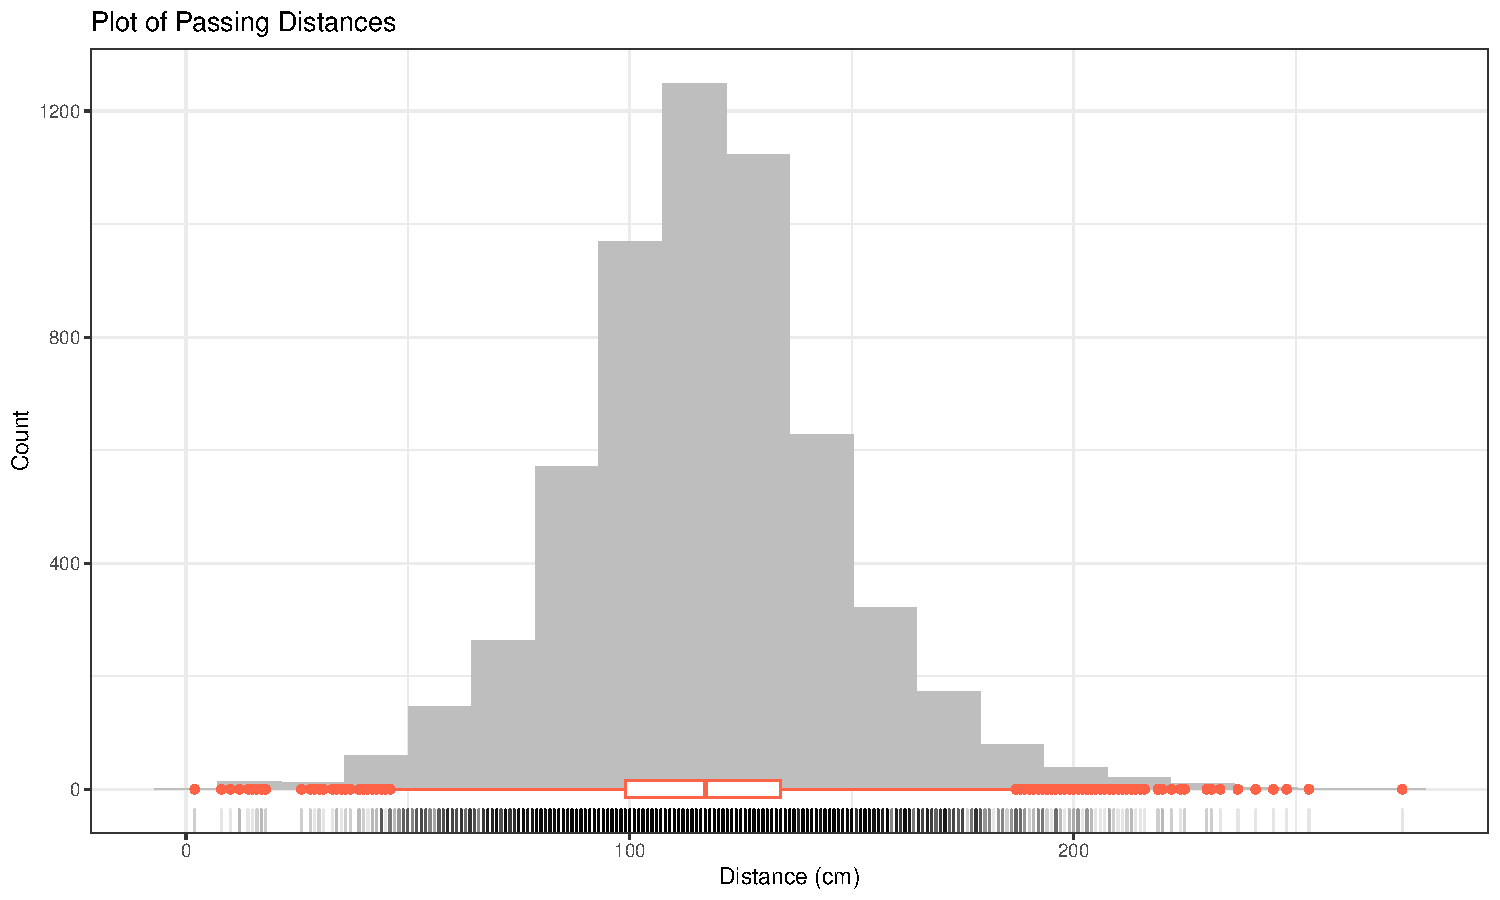
\includegraphics[width=0.75\linewidth]{02-linearmodelsreview_files/figure-latex/Figure2-1-1} 

}

\caption{Histogram (with 20 bins), boxplot, and rug of passing distances (in cm).}\label{fig:Figure2-1}
\end{figure}

\begin{Shaded}
\begin{Highlighting}[]
\NormalTok{dd }\SpecialCharTok{\%\textgreater{}\%} \FunctionTok{ggplot}\NormalTok{(}\AttributeTok{mapping =} \FunctionTok{aes}\NormalTok{(}\AttributeTok{x =}\NormalTok{ Distance)) }\SpecialCharTok{+}
  \FunctionTok{geom\_histogram}\NormalTok{(}\AttributeTok{bins =} \DecValTok{20}\NormalTok{, }\AttributeTok{fill =} \StringTok{"grey"}\NormalTok{) }\SpecialCharTok{+}
  \FunctionTok{geom\_rug}\NormalTok{(}\AttributeTok{alpha =} \FloatTok{0.1}\NormalTok{) }\SpecialCharTok{+}
  \FunctionTok{geom\_boxplot}\NormalTok{(}\AttributeTok{color =} \StringTok{"tomato"}\NormalTok{, }\AttributeTok{width =} \DecValTok{30}\NormalTok{) }\SpecialCharTok{+} 
      \CommentTok{\# width used to scale boxplot to make it more visible}
  \FunctionTok{theme\_bw}\NormalTok{() }\SpecialCharTok{+}
  \FunctionTok{labs}\NormalTok{(}\AttributeTok{title =} \StringTok{"Plot of Passing Distances"}\NormalTok{,}
       \AttributeTok{x =} \StringTok{"Distance (cm)"}\NormalTok{,}
       \AttributeTok{y =} \StringTok{"Count"}\NormalTok{)}
\end{Highlighting}
\end{Shaded}

\indent Based on Figure \ref{fig:Figure2-1}, the distribution appears to be relatively symmetric with many observations in both tails flagged as potential
outliers. Despite being flagged as potential outliers, they seem to be part of a common distribution. In real data sets, outliers are commonly encountered and the
first step is to verify that they were not errors in recording (if so, fixing or removing them is easily justified). If they cannot be easily dismissed or fixed, the next step
is to study their impact on the statistical analyses performed, potentially
considering reporting results with and without the influential observation(s)
in the results (if there are just handful). If the analysis is unaffected by the ``unusual'' observations,
then it matters little whether they are dropped or not. If they do affect the
results, then reporting both versions of results allows the reader to judge the
impacts for themselves. It is important to remember that sometimes the outliers
are the most interesting part of the data set. \index{outlier} For example, those observations that were the closest would be of great interest, whether they are outliers or not.

\indent Often when statisticians think of distributions of data, we think
of the smooth underlying
shape that led to the data set that is being displayed in the histogram.
Instead of binning up observations and making bars in the histogram, we can
estimate what is called a \textbf{\emph{density curve}} as a smooth curve
that represents the observed distribution of the responses. Density curves can
sometimes help us see features of the data sets more clearly. \index{density curve}

\indent To understand the density curve, it is useful to initially see
the histogram and density curve together. The height of the density curve is scaled
so that the total area under the curve\footnote{If you've taken calculus, you will
  know that the
  curve is being constructed so that the integral from \(-\infty\) to
  \(\infty\) is 1. If you don't know calculus, think of a rectangle with area
  of 1 based on its height and width. These cover the same area but the top of the
  region wiggles.} is 1. To make a comparable histogram, the
y-axis needs to be scaled so that the histogram is also on the ``density''
scale which makes the bar heights adjust so that the proportion of the
total data set in each bar is represented by the area in each bar
(remember that area is height times width). So the height depends on the
width of the bars and the total area across all the bars has to be 1. In the
\texttt{geom\_histogram}, its aesthetic is modified using the (cryptic\footnote{I admit that there are parts of the logic of using \texttt{ggplot} that are confusing to me and this is one of them -- but I learned to plot in R before \texttt{ggplot2} and have been growing fonder and fonder of this way of working. Now instead of searching the internet, I will just get to search my book for the code to make this version of the plot.}) code of \texttt{(y\ =\ ..density..)}. The
density curve is added to the histogram using the \texttt{geom\_density}, producing the result in Figure \ref{fig:Figure2-2} with
added modifications for filling the density curve but using \texttt{alpha\ =\ 0.1} to make the density curve fill transparent (alpha values range between 0 and 1 with lower values providing more transparency) and in purple (\texttt{fill\ =\ purple}). You can see how the density curve
somewhat matches the histogram bars but deals with the bumps up and down
and edges a little differently. We can pick out the relatively symmetric distribution using
either display and will rarely make both together. \index{\texttt{geom\_density()}}



\begin{figure}[ht!]

{\centering 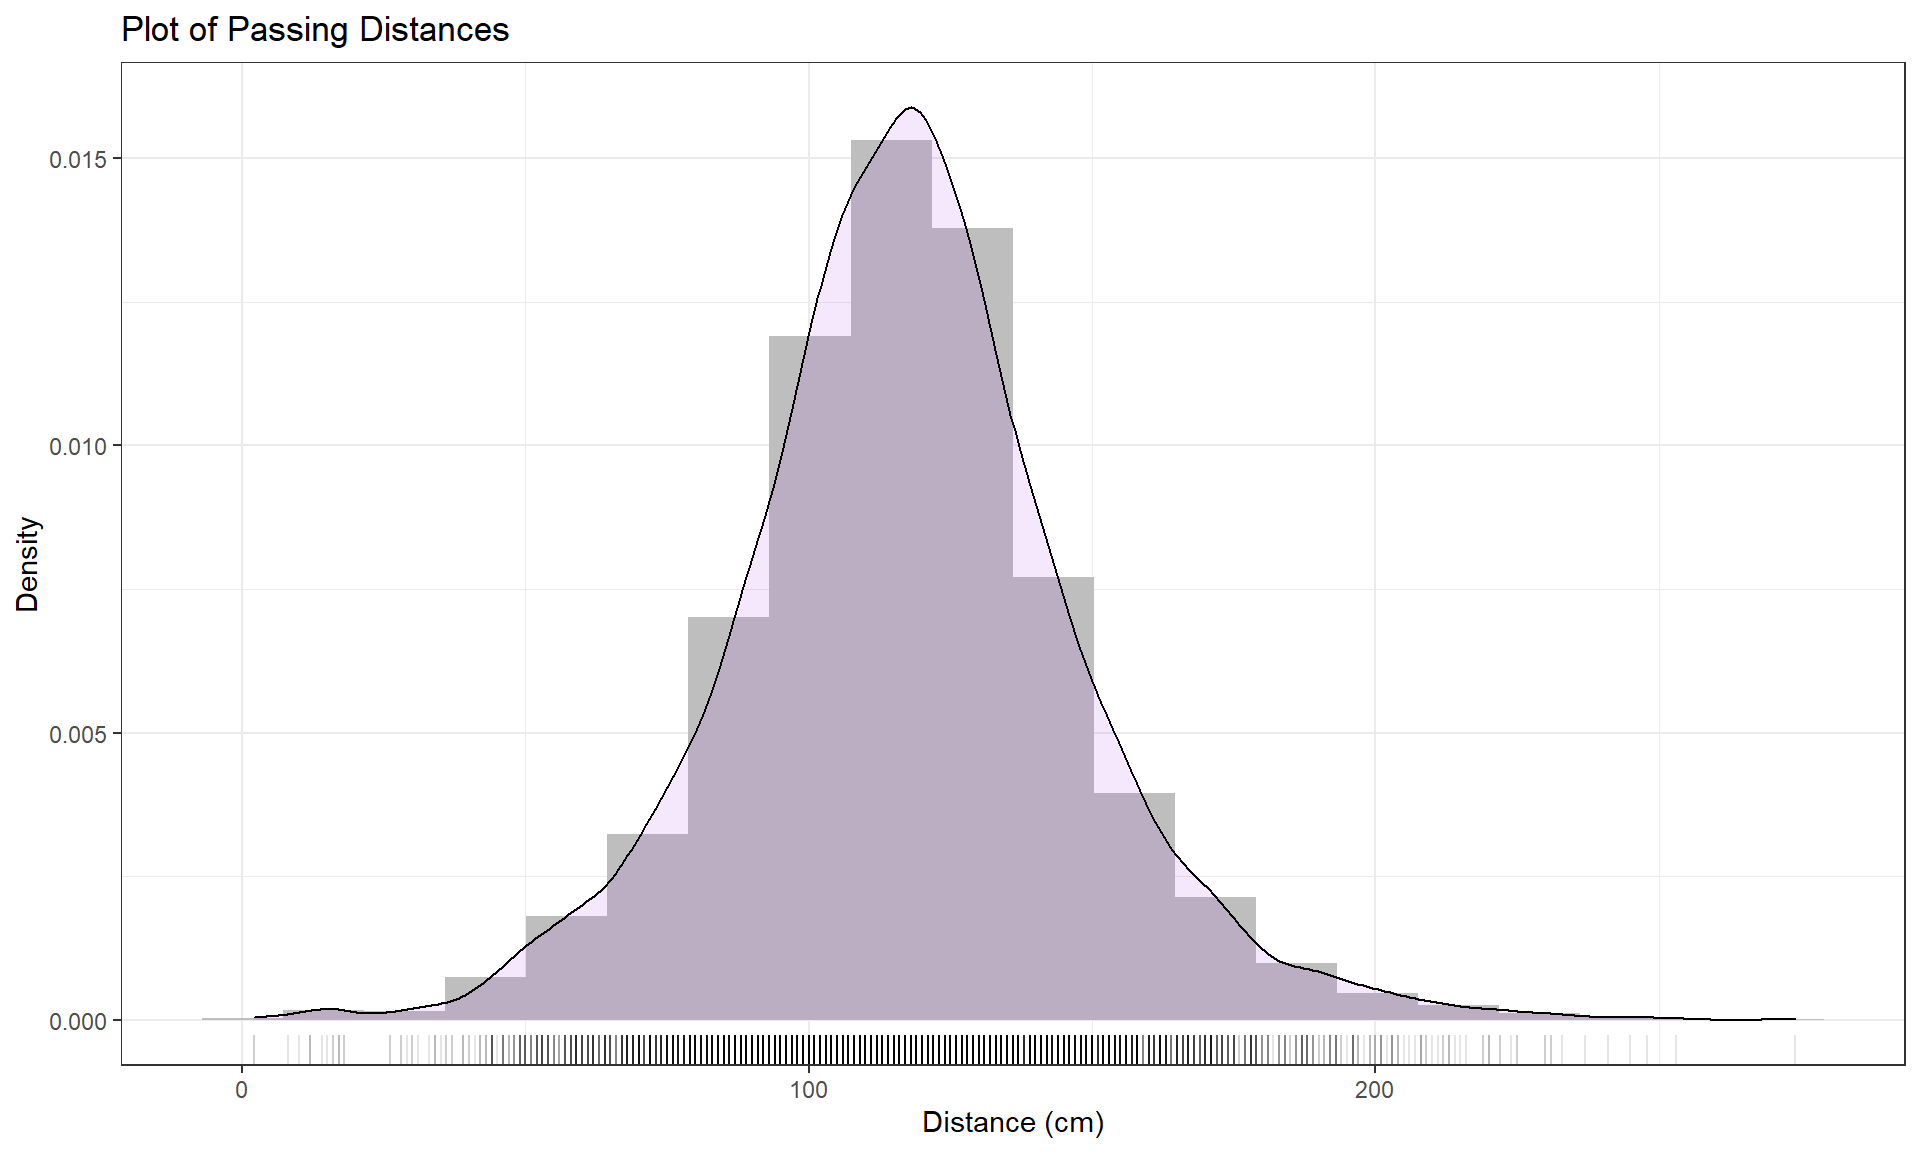
\includegraphics[width=0.75\linewidth]{02-linearmodelsreview_files/figure-latex/Figure2-2-1} 

}

\caption{Histogram (density scaled), density curve, and rug plot of Distance responses.}\label{fig:Figure2-2}
\end{figure}

\begin{Shaded}
\begin{Highlighting}[]
\NormalTok{dd }\SpecialCharTok{\%\textgreater{}\%} \FunctionTok{ggplot}\NormalTok{(}\AttributeTok{mapping =} \FunctionTok{aes}\NormalTok{(}\AttributeTok{x =}\NormalTok{ Distance)) }\SpecialCharTok{+}
  \FunctionTok{geom\_histogram}\NormalTok{(}\AttributeTok{bins =} \DecValTok{15}\NormalTok{, }\AttributeTok{fill =} \StringTok{"grey"}\NormalTok{, }\FunctionTok{aes}\NormalTok{(}\AttributeTok{y =}\NormalTok{ ..density..)) }\SpecialCharTok{+}
  \FunctionTok{geom\_density}\NormalTok{(}\AttributeTok{fill =} \StringTok{"purple"}\NormalTok{, }\AttributeTok{alpha =} \FloatTok{0.1}\NormalTok{) }\SpecialCharTok{+} 
  \FunctionTok{geom\_rug}\NormalTok{(}\AttributeTok{alpha =} \FloatTok{0.1}\NormalTok{) }\SpecialCharTok{+} 
  \FunctionTok{theme\_bw}\NormalTok{() }\SpecialCharTok{+}
  \FunctionTok{labs}\NormalTok{(}\AttributeTok{title =} \StringTok{"Plot of Passing Distances"}\NormalTok{,}
       \AttributeTok{x =} \StringTok{"Distance (cm)"}\NormalTok{,}
       \AttributeTok{y =} \StringTok{"Density"}\NormalTok{)}
\end{Highlighting}
\end{Shaded}

\indent Histograms can be sensitive to the choice of the number of bars and
even the cut-offs used to define the bins for a given number of bars.
Small changes in the definition of cut-offs for the bins can have
noticeable impacts on the shapes observed but
this does not impact density curves. We have engaged the arbitrary choice of the number of bins, but we can add information on the original observations being included in each bar to better understand the choices that \texttt{geom\_hist} is making. We can (barely) see how there are 2 observations at 2 cm (the noise
added generates a wider line than for an individual observation so it is possible to see that it is more than one observation there but I had to check the data set to confirm this). A limitation of the
histogram arises at the center of the distribution where the bar that goes from approximately 110 to 120 cm suggests that the mode (peak) is in this range (but it is unclear where) but the density curve suggests that the peak is closer to 120 than 110. Both density curves and histograms can react to individual points in the tails of distributions, but sometimes in different ways.

\indent The graphical tools we've just discussed are going to help us move to comparing the
distribution of responses across more than one group. We will have two displays
that will help us make these comparisons. The simplest is
the \textbf{\emph{side-by-side boxplot}}, where a boxplot is displayed for each group
of interest using the same y-axis scaling. \index{boxplot} In the base R \texttt{boxplot} function, we can use its \textbf{\emph{formula}}
notation to see if the response (\texttt{Distance}) differs based on the group
(\texttt{Condition}) by using something like \texttt{Y\ \textasciitilde{}\ X} or, here, \texttt{Distance\ \textasciitilde{}\ Condition}.
We also need to tell R where to find the variables -- use the last option in the command, \texttt{data\ =\ DATASETNAME} , to inform R of the tibble to look in
to find the variables. In this example, \texttt{data\ =\ dd}. We will use
the formula and \texttt{data\ =\ ...} options in almost every function we use
from here forward, except in \texttt{ggplot} which has too many options for formulas to be useful.

\indent Figure \ref{fig:Figure2-3} contains the side-by-side
boxplots showing similar distributions for all the groups, with a slightly higher median in the ``police'' group and some potential outliers identified in both tails of the distributions in all groups.



\begin{figure}[ht!]

{\centering 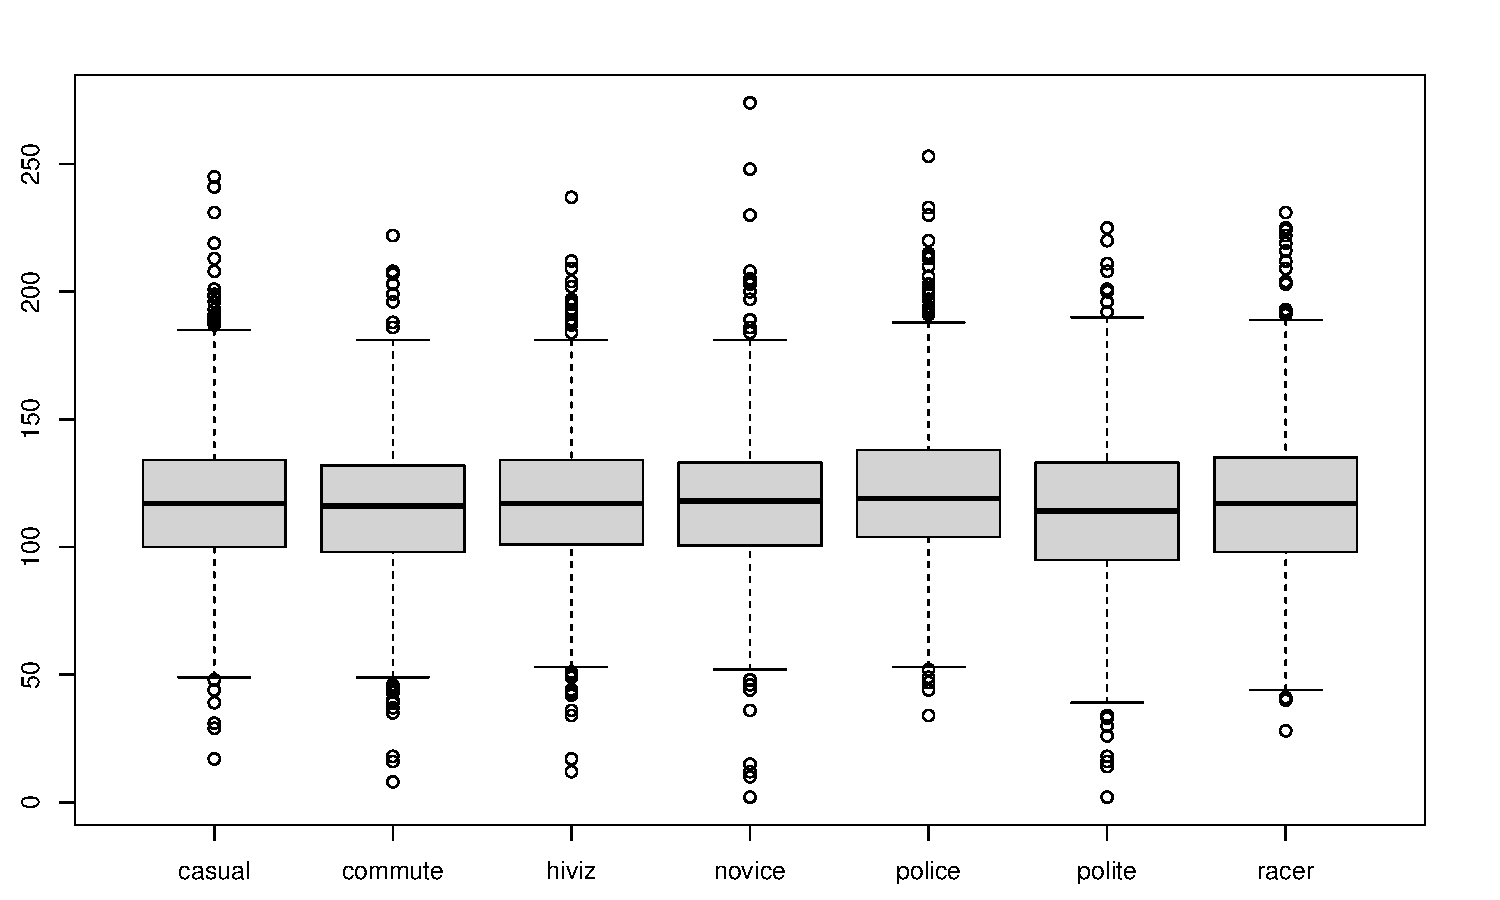
\includegraphics[width=0.75\linewidth]{02-linearmodelsreview_files/figure-latex/Figure2-3-1} 

}

\caption{Side-by-side boxplot of distances based on outfits.}\label{fig:Figure2-3}
\end{figure}

\begin{Shaded}
\begin{Highlighting}[]
\FunctionTok{boxplot}\NormalTok{(Distance }\SpecialCharTok{\textasciitilde{}}\NormalTok{ Condition, }\AttributeTok{data =}\NormalTok{ dd)}
\end{Highlighting}
\end{Shaded}

\indent The ``\textasciitilde{}'' (which is read as the \emph{tilde} symbol\footnote{If you want to type this character in R Markdown, try \texttt{\$\textbackslash{}sim\$} outside of code chunks.}, which you can find in the
upper left corner of your keyboard) notation will be used in two ways in this
material. \index{tilde} The formula use in R employed previously declares that the
response variable here is \emph{Distance} and the explanatory variable is \emph{Condition}.
The other use for ``\textasciitilde{}'' is as shorthand for ``is distributed as'' and is used in
the context of \(Y \sim N(0,1)\), which translates (in statistics) to defining the
random variable \emph{Y} as following a Normal distribution\footnote{Remember the
  bell-shaped curve you encountered in introductory statistics? If not, you can
  see some at \url{https://en.wikipedia.org/wiki/Normal_distribution}.}
\index{normal distribution}
with mean 0
and variance of 1 (which also means that the standard deviation is 1). In the current situation, we could ask whether
the \texttt{Distance} variable seems like it may follow a normal distribution in each group, in
other words, is \(\text{Distance}\sim N(\mu,\sigma^2)\)? Since the responses are relatively symmetric, it is not clear that we have a violation of the assumption of the normality assumption for the \emph{Distance} variable for any of the seven groups (more later on how we can assess this and the issues that occur when we have a violation of this assumption). Remember that
\(\mu\) and \(\sigma\) are parameters where
\(\mu\) (``mu'') is our standard symbol for the \textbf{\emph{population mean}}
and that \(\sigma\) (``sigma'') is the symbol of the
\textbf{\emph{population standard deviation}} and \(\sigma^2\) is the symbol of the
\textbf{\emph{population variance}}. \index{mean} \index{standard deviation}

\hypertarget{section2-2}{%
\section{Pirate-plots}\label{section2-2}}

An alternative graphical display for comparing multiple groups that we will use is a display called a \textbf{\emph{pirate-plot}} (\protect\hyperlink{ref-R-yarrr}{Phillips 2017}) from the \texttt{yarrr} package\footnote{The package and function are intentionally amusingly titled but are based on ideas in the beanplot in Kampstra (\protect\hyperlink{ref-Kampstra2008}{2008}) and provide what they call an \textbf{\emph{RDI graphic}} -- \textbf{\emph{R}}aw data, \textbf{\emph{D}}escriptive, and \textbf{\emph{I}}nferential statistic in the same display.}. \index{pirate-plot} Figure \ref{fig:Figure2-4}
shows an example of a pirate-plot that provides a side-by-side display that
contains the density curves, the original observations that generated the
density curve as jittered points (jittered both vertically and horizontally a little), the sample mean of each group (wide bar), and vertical lines to horizontal bars that represents the confidence interval for the true mean of that group. For each group, the density curves
are mirrored to aid in visual assessment of the shape of the distribution. This mirroring also
creates a shape that resembles the outline of a violin with skewed distributions so versions of this
display have also been called a ``violin plot'' or a ``bean plot'' (I call these ``enhanced violin plots'' when I use them in journal articles instead of ``pirate plots''). All together this plot shows us information
on the original observations, center (mean) and its confidence interval, spread, and shape of the distributions of the responses. Our inferences typically focus on the means of the groups and this plot allows
us to compare those across the groups while gaining information on the shapes
of the distributions of responses in each group.

\indent To use the \texttt{pirateplot} function \index{\texttt{pirateplot()}} we need to install and then load the \texttt{yarrr}
package.
\index{R packages!\textbf{yarrr}}
The function works like the boxplot used previously
except that options
for the type of confidence interval needs to be specified with \texttt{inf.method\ =\ "ci"} -- otherwise you will get a different kind of interval than you learned in introductory statistics and we don't want to get caught up in trying to understand the kind of interval it makes by default. And it seems useful to add \texttt{inf.disp\ =\ "line"} as an additional option to add bars for the confidence interval\footnote{The default version seems to get mis-interpreted as the box from a boxplot too easily. This display choice also matches the display style for later plots for confidence intervals in term-plots.}. There are many other options in the function that might be useful in certain situations, but these are the only ones that are really needed to get started with pirate-plots. While we could build this plot using \texttt{ggplot}, the simplicity of this function keeps it a favorite way to display a quantitative variable across groups even though we lose the grammar of graphics way of modifying the plot.



\begin{figure}[ht!]

{\centering 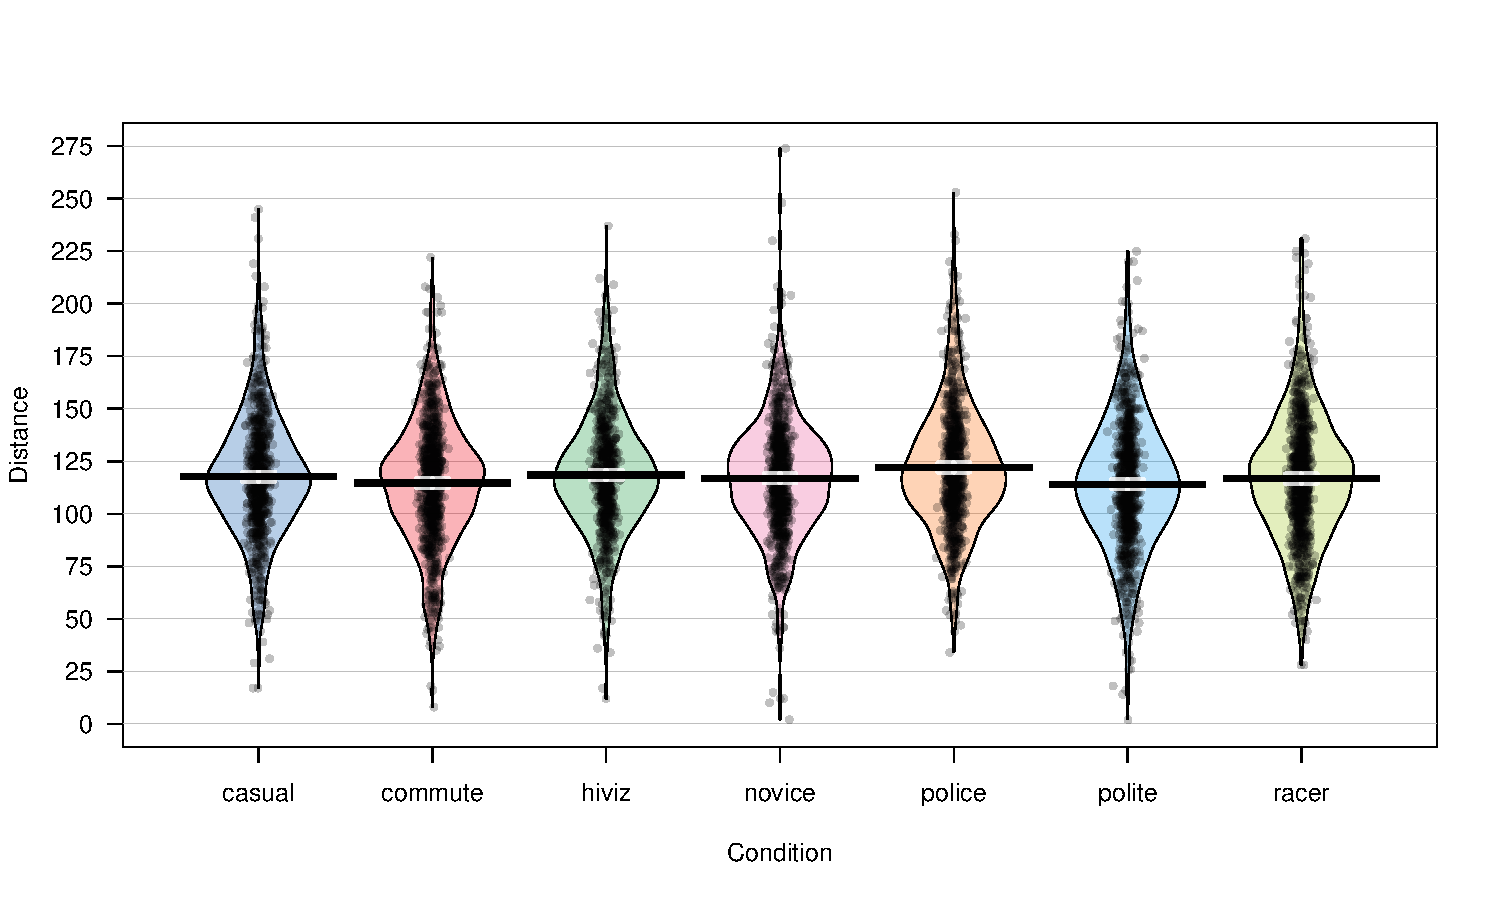
\includegraphics[width=0.75\linewidth]{02-linearmodelsreview_files/figure-latex/Figure2-4-1} 

}

\caption{Pirate-plot of distances by outfit group. Bold horizontal lines correspond to sample mean of each group, boxes around lines (here they are very tight to the lines for the means) are the 95\% confidence intervals.}\label{fig:Figure2-4}
\end{figure}

\begin{Shaded}
\begin{Highlighting}[]
\FunctionTok{library}\NormalTok{(yarrr)}
\FunctionTok{pirateplot}\NormalTok{(Distance }\SpecialCharTok{\textasciitilde{}}\NormalTok{ Condition, }\AttributeTok{data =}\NormalTok{ dd, }\AttributeTok{inf.method =} \StringTok{"ci"}\NormalTok{, }\AttributeTok{inf.disp =} \StringTok{"line"}\NormalTok{)}
\end{Highlighting}
\end{Shaded}

Figure \ref{fig:Figure2-4} suggests that the distributions are relatively symmetric which would suggest that the means and medians are similar even though only the means are displayed in these plots. In this display, none of the observations are flagged as outliers (it is not a part of this display). It is up to the consumer of the graphic to decide if observations look to be outside of the overall pattern of the rest of the observations. By plotting the observations by groups, we can also explore the narrowest (and likely most scary) overtakes in the data set. The \emph{police} and \emph{racer} conditions seem to have all observations over 25 cm and the most close passes were in the \emph{novice} and \emph{polite} outfits, including the two 2 cm passes. By displaying the original observations, we are able to explore and identify features that aggregation and summarization in plots can sometimes obfuscate. But the pirate-plots also allow you to compare the shape of the distributions (relatively symmetric and somewhat bell-shaped), variability (they look to have relatively similar variability), and the means of the groups. Our inferences are going to focus on the means but those inferences are only valid if the distributions are either approximately normal or at least have similar shapes and spreads (more on this soon).

\indent It appears that the mean for \emph{police} is higher than the other groups but that the others are not too different. But is this difference real? We will never
know the answer to that question, but we
can assess how likely we are to have seen a result as extreme or more
extreme than our result, assuming that there is no difference in the
means of the groups. And if the observed result is
(extremely) unlikely to occur, then we have (extremely) strong evidence against the hypothesis that the
groups have the same mean and can then conclude that there is likely a real
difference. If we discover that our result was not very unlikely, given the assumption of no difference in the mean of the groups, then we can't conclude that there is a difference but also can't conclude that they are equal, just that we failed to find enough evidence against the equal means assumption to discard it as a possibility. Whether the result is unusual or not, we will want to carefully explore how big the estimated differences in the means are -- is the difference in means large enough to matter to you? We would be more interested in the implications of the difference in the means when there is strong evidence against the null hypothesis that the means are equal but the size of the estimated differences should always be of some interest. To accompany the pirate-plot that displays estimated means, we
need to have numerical values to compare. We can get means and standard
deviations by groups easily using the same formula notation as for the plots with the \texttt{mean}
and \texttt{sd} functions, if the \texttt{mosaic} package is loaded.

\begin{Shaded}
\begin{Highlighting}[]
\FunctionTok{library}\NormalTok{(mosaic)}
\FunctionTok{mean}\NormalTok{(Distance }\SpecialCharTok{\textasciitilde{}}\NormalTok{ Condition, }\AttributeTok{data =}\NormalTok{ dd)}
\end{Highlighting}
\end{Shaded}

\begin{verbatim}
##   casual  commute    hiviz   novice   police   polite    racer 
## 117.6110 114.6079 118.4383 116.9405 122.1215 114.0518 116.7559
\end{verbatim}

\begin{Shaded}
\begin{Highlighting}[]
\FunctionTok{sd}\NormalTok{(Distance }\SpecialCharTok{\textasciitilde{}}\NormalTok{ Condition, }\AttributeTok{data =}\NormalTok{ dd)}
\end{Highlighting}
\end{Shaded}

\begin{verbatim}
##   casual  commute    hiviz   novice   police   polite    racer 
## 29.86954 29.63166 29.03384 29.03812 29.73662 31.23684 30.60059
\end{verbatim}

We can also use the \texttt{favstats} function to get those summaries and others by groups.

\begin{Shaded}
\begin{Highlighting}[]
\FunctionTok{favstats}\NormalTok{(Distance }\SpecialCharTok{\textasciitilde{}}\NormalTok{ Condition, }\AttributeTok{data =}\NormalTok{ dd)}
\end{Highlighting}
\end{Shaded}

\begin{verbatim}
##   Condition min    Q1 median  Q3 max     mean       sd   n missing
## 1    casual  17 100.0    117 134 245 117.6110 29.86954 779       0
## 2   commute   8  98.0    116 132 222 114.6079 29.63166 857       0
## 3     hiviz  12 101.0    117 134 237 118.4383 29.03384 737       0
## 4    novice   2 100.5    118 133 274 116.9405 29.03812 807       0
## 5    police  34 104.0    119 138 253 122.1215 29.73662 790       0
## 6    polite   2  95.0    114 133 225 114.0518 31.23684 868       0
## 7     racer  28  98.0    117 135 231 116.7559 30.60059 852       0
\end{verbatim}

\indent Based on these results, we can see that there is an estimated difference of over 8 cm between the smallest mean (\emph{polite} at 114.05 cm) and the largest mean (\emph{police} at 122.12 cm). The differences among some of the other groups are much smaller, such as between \emph{casual} and \emph{commute} with sample means of 117.611 and 114.608 cm, respectively. Because there are seven groups being compared in this study, we will have to
wait until Chapter 3 and the One-Way ANOVA test to fully assess evidence
related to some difference among the seven groups. For now, we are going to
focus on comparing the mean \emph{Distance} between \emph{casual} and \emph{commute} groups
-- which is a \textbf{\emph{two independent sample mean}} situation and something you
should have seen before. Remember that the ``independent'' sample part of
this refers to observations that are independently observed for the two
groups as opposed to the paired sample situation that you may have
explored where one observation from the first group is related to an
observation in the second group (the same person with one measurement in each group (we
generically call this ``repeated measures'')
or the famous ``twin'' studies with one twin assigned to each group). \index{two independent sample mean} This study has some potential violations of the ``independent'' sample situation (for example, repeated measurements made during a single ride), but those do not clearly fit into the matched pairs situation, so we will note this potential issue and proceed with exploring the method that assumes that we have independent samples, even though this is not true here. In Chapter 9, methods for more complex study designs like this one will be discussed briefly, but mostly this is beyond the scope of this material.

\indent Here we are going to use the ``simple'' two independent group scenario to
review some basic statistical concepts and connect two different
frameworks for conducting statistical inference: randomization and
parametric \index{parametric} inference techniques. \textbf{\emph{Parametric}} statistical methods
involve making assumptions
\index{assumptions}
about the distribution of the
responses and obtaining confidence intervals and/or p-values using a
\emph{named} distribution (like the \(z\) or \(t\)-distributions). Typically these
results are generated using formulas and looking up areas under curves or
cutoffs using a table or a computer. \textbf{\emph{Randomization}}-based statistical
methods use a computer to shuffle, sample, or simulate observations in ways
that allow you to obtain distributions of possible results to find areas and
cutoffs without resorting to using tables and named distributions.
Randomization methods are what are called \textbf{\emph{nonparametric}} methods
\index{nonparametric}
that often make fewer assumptions (they are \textbf{\emph{not free of assumptions}}!)
and so can handle a larger set of problems more easily than parametric
methods.
\index{assumptions}
When the assumptions involved in the parametric procedures are
met by a data set, the randomization methods often provide very similar
results to those provided by the parametric techniques. To be a more
sophisticated statistical consumer, it is useful to have some knowledge
of both of these techniques for performing statistical inference and the fact that they can provide similar results might deepen your understanding of both
approaches.

\indent To be able to work just with the observations from two of the conditions (\emph{casual} and \emph{commute}) we could remove all the other observations in a spreadsheet program and read that new data set
back into R, but it is actually pretty easy to use R to do data
management once the data set is loaded. It is also a better scientific process to do as much of your data management within R as possible so that your steps in managing the data are fully documented and reproducible. Highlighting and clicking in spreadsheet programs is a dangerous way to work and can be impossible to recreate steps that were taken from initial data set to the version that was analyzed. In R, we could identify the rows that contain the observations we want to retain and just extract those rows, but this is hard with over five thousand observations. The \texttt{filter} function from the \texttt{dplyr} package (part of the \texttt{tidyverse} suite of packages) is the best way to be able to focus on observations that meet a particular condition; we can ``filter'' the data set to retain just those rows. The \texttt{filter} function takes the data set via the pipe operate and then we need to define the condition we want to meet to retain those rows. Here we need to define the variable we want to work with, \texttt{Condition}, and then request rows that meet a condition (are \texttt{\%in\%}) and the aspects that meet that condition (here by concatenating the two levels of ``casual'' and ``commute''), leading to code of: \index{\texttt{filter()}}

\begin{verbatim}
dd %>% filter(Condition %in% c("casual", "commute"))
\end{verbatim}

We want to save that new filtered data set into a new tibble for future work, so we can use the assignment operator (\texttt{\textless{}-}) to save the reduced data set into \texttt{ddsub}:

\begin{Shaded}
\begin{Highlighting}[]
\NormalTok{ddsub }\OtherTok{\textless{}{-}}\NormalTok{ dd }\SpecialCharTok{\%\textgreater{}\%} \FunctionTok{filter}\NormalTok{(Condition }\SpecialCharTok{\%in\%} \FunctionTok{c}\NormalTok{(}\StringTok{"casual"}\NormalTok{, }\StringTok{"commute"}\NormalTok{))}
\end{Highlighting}
\end{Shaded}

There is also the \texttt{select} function that we could also use with an additional pipe operator to just focus on certain columns in the data set, here to just retain the \texttt{Condition} and \texttt{Distance} variables using: \index{\texttt{select()}}

\begin{Shaded}
\begin{Highlighting}[]
\NormalTok{ddsub }\OtherTok{\textless{}{-}}\NormalTok{ dd }\SpecialCharTok{\%\textgreater{}\%} 
  \FunctionTok{filter}\NormalTok{(Condition }\SpecialCharTok{\%in\%} \FunctionTok{c}\NormalTok{(}\StringTok{"casual"}\NormalTok{,}\StringTok{"commute"}\NormalTok{)) }\SpecialCharTok{\%\textgreater{}\%}
  \FunctionTok{select}\NormalTok{(Distance, Condition)}
\end{Highlighting}
\end{Shaded}

The \texttt{select} function shows up in multiple packages so you might need to use \texttt{dplyr::select()} which tells R to use the version of \texttt{select} that is in \texttt{dplyr}. When you are working to filter or subset your data set you should always check that the correct observations were dropped
either using \texttt{View(ddsub)} or by doing a quick summary of the
\texttt{Condition} variable in the new tibble.

\begin{Shaded}
\begin{Highlighting}[]
\FunctionTok{summary}\NormalTok{(ddsub}\SpecialCharTok{$}\NormalTok{Condition)}
\end{Highlighting}
\end{Shaded}

\begin{verbatim}
##  casual commute   hiviz  novice  police  polite   racer 
##     779     857       0       0       0       0       0
\end{verbatim}

It ends up that R remembers the categories for observations that we removed even though there are
0 observations in them now and that can cause us some problems. When we remove a
group of observations, we sometimes need to clean up categorical variables to
just reflect the categories that are present. The \texttt{factor}
\index{\texttt{factor()}}
function
creates categorical variables based on the levels of the variables that are
observed and is useful to run here to clean up \texttt{Condition} to just reflect the categories that are now present.

\begin{Shaded}
\begin{Highlighting}[]
\NormalTok{ddsub }\OtherTok{\textless{}{-}}\NormalTok{ ddsub }\SpecialCharTok{\%\textgreater{}\%} \FunctionTok{mutate}\NormalTok{(}\AttributeTok{Condition =} \FunctionTok{factor}\NormalTok{(Condition))}
\FunctionTok{summary}\NormalTok{(ddsub}\SpecialCharTok{$}\NormalTok{Condition)}
\end{Highlighting}
\end{Shaded}

\begin{verbatim}
##  casual commute 
##     779     857
\end{verbatim}

\indent The two categories of interest now were selected because neither looks particularly ``racey'' or has high visibility but could present a common choice between getting fully ``geared up'' for the commute or just jumping on a bike to go to work. Now if we remake the boxplots and pirate-plots, they only contain results for
the two groups of interest here as seen in Figure \ref{fig:Figure2-5}. Note that these are available in the previous version of the plots, but now we will just focus on these two groups.



\begin{figure}[ht!]

{\centering 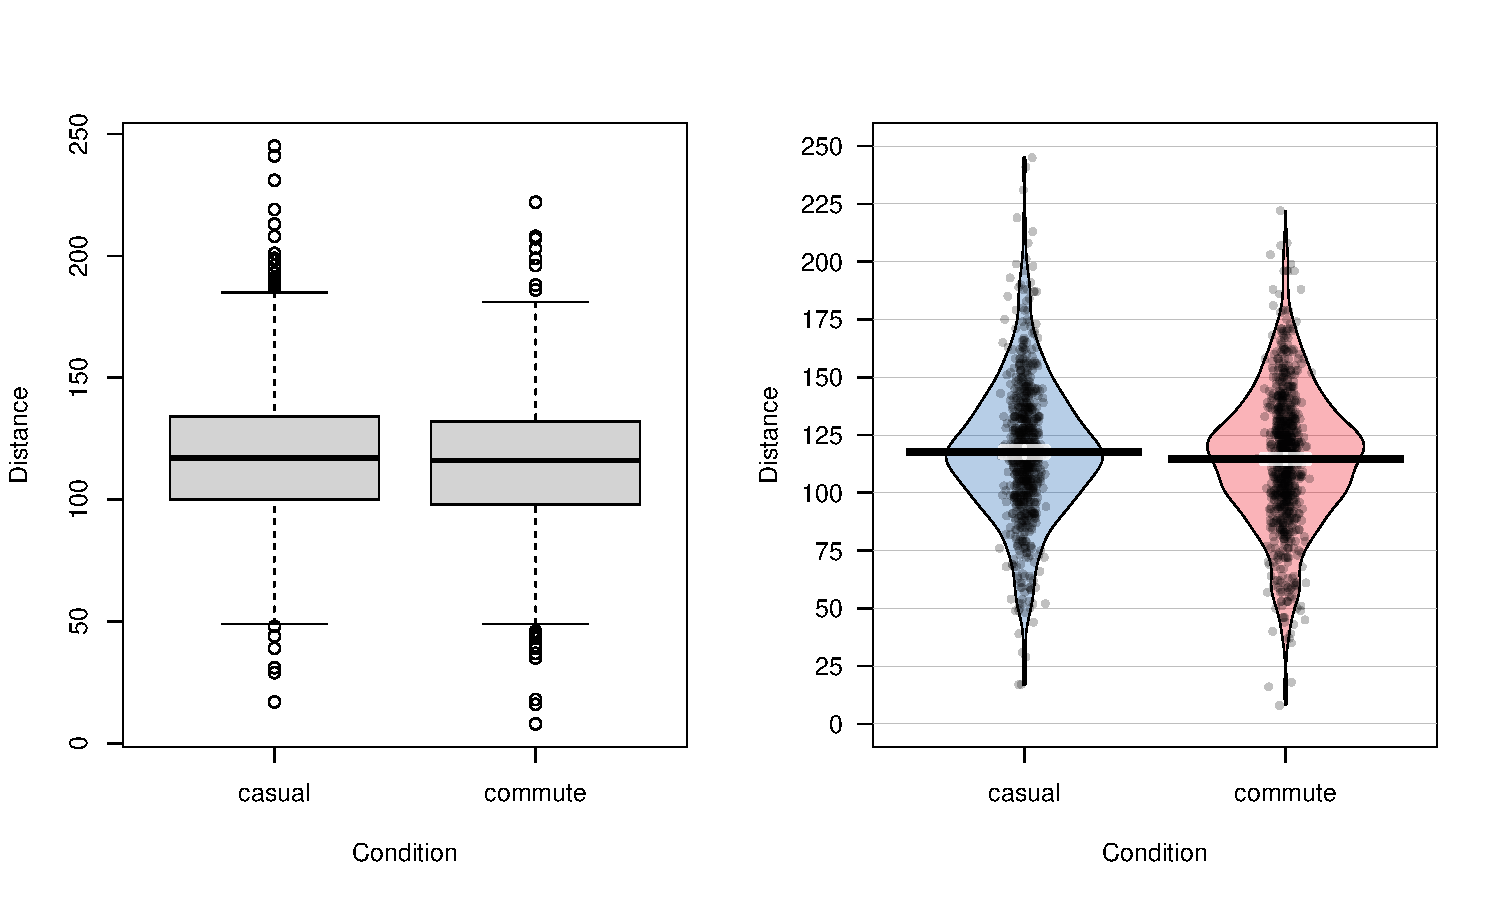
\includegraphics[width=0.75\linewidth]{02-linearmodelsreview_files/figure-latex/Figure2-5-1} 

}

\caption{Boxplot and pirate-plot of the \emph{Distance} responses on the reduced \texttt{ddsub} data set.}\label{fig:Figure2-5}
\end{figure}

\begin{Shaded}
\begin{Highlighting}[]
\FunctionTok{boxplot}\NormalTok{(Distance }\SpecialCharTok{\textasciitilde{}}\NormalTok{ Condition, }\AttributeTok{data =}\NormalTok{ ddsub) }
\FunctionTok{pirateplot}\NormalTok{(Distance }\SpecialCharTok{\textasciitilde{}}\NormalTok{ Condition, }\AttributeTok{data =}\NormalTok{ ddsub, }\AttributeTok{inf.method =} \StringTok{"ci"}\NormalTok{, }\AttributeTok{inf.disp =} \StringTok{"line"}\NormalTok{)}
\end{Highlighting}
\end{Shaded}

\indent The two-sample mean techniques you learned in your previous course all
start with comparing the means the two groups. We can obtain the two
means using the \texttt{mean} function or directly obtain the difference
in the means using the \texttt{diffmean} function (both require the \texttt{mosaic}
package). The \texttt{diffmean} function provides
\(\bar{x}_\text{commute} - \bar{x}_\text{casual}\) where \(\bar{x}\)
(read as ``x-bar'') is the sample mean of observations in the subscripted
group. Note that there are two directions that you could compare the
means and this function chooses to take the mean from the second group
name \emph{alphabetically} and subtract the mean from the first alphabetical group
name. It is always good to check the direction of this calculation as
having a difference of \(-3.003\) cm versus \(3.003\) cm could be important.

\begin{Shaded}
\begin{Highlighting}[]
\FunctionTok{mean}\NormalTok{(Distance }\SpecialCharTok{\textasciitilde{}}\NormalTok{ Condition, }\AttributeTok{data =}\NormalTok{ ddsub)}
\end{Highlighting}
\end{Shaded}

\begin{verbatim}
##   casual  commute 
## 117.6110 114.6079
\end{verbatim}

\begin{Shaded}
\begin{Highlighting}[]
\FunctionTok{diffmean}\NormalTok{(Distance }\SpecialCharTok{\textasciitilde{}}\NormalTok{ Condition, }\AttributeTok{data =}\NormalTok{ ddsub)}
\end{Highlighting}
\end{Shaded}

\begin{verbatim}
##  diffmean 
## -3.003105
\end{verbatim}

\hypertarget{section2-3}{%
\section{Models, hypotheses, and permutations for the two sample mean situation}\label{section2-3}}

There appears to be some evidence that the \emph{casual} clothing group is
getting higher average overtake distances than
the \emph{commute} group of observations, but we want to try to make sure that the difference is
real -- to assess evidence against the assumption that the means
are the same ``in the population'' and possibly decide that this is not a reasonable assumption. First, a \textbf{\emph{null hypothesis}}\footnote{The
  hypothesis of no difference that is typically generated in the hopes of
  being rejected in favor of the alternative hypothesis, which contains the sort
  of difference that is of interest in the application.} which
defines a \textbf{\emph{null model}}\footnote{The null model is the statistical model that
  is implied by the chosen null hypothesis. Here, a null hypothesis of no
  difference translates to having a model with the same mean for both groups.}
\index{model!null}
needs to be determined in terms of \textbf{\emph{parameters}} (the true values in
the population). The research question should help you determine the form of the
hypotheses for the assumed population. In the two independent sample mean
problem, the interest is in testing a null hypothesis of \(H_0: \mu_1 = \mu_2\)
versus the alternative hypothesis of \(H_A: \mu_1 \ne \mu_2\), where
\(\mu_1\) is the parameter for the true mean of the first group and \(\mu_2\)
is the parameter for the true mean of the second group. The alternative
hypothesis involves assuming a statistical model
\index{model!two independent sample mean}
for the \(i^{th}\ (i = 1,\ldots,n_j)\)
response from the \(j^{th}\ (j = 1,2)\) group, \(\boldsymbol{y}_{ij}\), that
involves modeling it as \(y_{ij} = \mu_j + \varepsilon_{ij}\),
where we assume that \(\varepsilon_{ij} \sim N(0,\sigma^2)\). For the moment,
focus on the models that either assume the means are the same (null) or
different (alternative),
\index{model!alternative}
which imply:

\begin{itemize}
\item
  Null Model: \(y_{ij} = \mu + \varepsilon_{ij}\) There is \textbf{no}
  difference in \textbf{true} means for the two groups.
\item
  Alternative Model: \(y_{ij} = \mu_j + \varepsilon_{ij}\) There is \textbf{a}
  difference in \textbf{true} means for the two groups.
\end{itemize}

Suppose we are considering the alternative model for the 4\textsuperscript{th}
observation (\(i = 4\)) from the second group (\(j = 2\)), then the model for
this observation is \(y_{42} = \mu_2 +\varepsilon_{42}\), that defines the
response as coming from the true mean for the second group plus a
random error term for that observation, \(\varepsilon_{42}\). For, say, the
5\textsuperscript{th} observation from the first group (\(j = 1\)), the model is
\(y_{51} = \mu_1 +\varepsilon_{51}\). If we were working with the null model,
the mean is always the same (\(\mu\)) -- the group specified does not change
the mean we use for that observation, so the model for \(y_{42}\) would be \(\mu +\varepsilon_{42}\).

\indent It can be helpful to think about the null and alternative models graphically.
\index{model!two-independent sample mean}
By assuming the null hypothesis is true (means are equal) and that the random
errors around the mean follow a normal distribution,
\index{normal distribution}
we assume that the truth
is as displayed in the left panel of Figure \ref{fig:Figure2-6} -- two
normal distributions with the same mean and variability. The alternative
model allows the two groups to potentially have different means, such as
those displayed in the right panel of Figure \ref{fig:Figure2-6} where the
second group has a larger mean. Note that in this scenario, we assume that
the observations all came from the same distribution except that they had
different means. Depending on the statistical procedure we are using, we
basically are going to assume that the observations (\(y_{ij}\)) either were
generated as samples from the null or alternative model. You can imagine
drawing observations at random from the pictured distributions. For hypothesis
testing, the null model
\index{model!null}
is assumed to be true and then the unusualness of
the actual result is assessed relative to that assumption. In hypothesis
testing, we have to decide if we have enough evidence to reject the assumption
that the null model (or hypothesis) is true. If we think that we have sufficient evidence to conclude that the null hypothesis is wrong,
then we would conclude that the other model considered (the alternative
model)
\index{model!alternative}
is more reasonable. The researchers obviously would have hoped to
encounter some sort of noticeable difference in the distances for the
different outfits and have been able to find enough evidence to against the null
model where the groups ``look the same'' to be able to conclude that they differ.



\begin{figure}[ht!]

{\centering 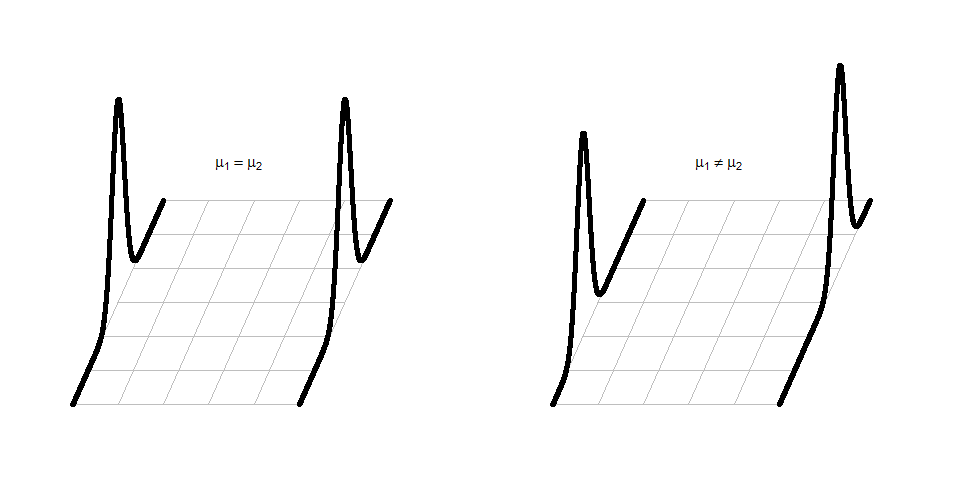
\includegraphics[width=1\linewidth]{chapter2_files/image015} 

}

\caption{Illustration of the assumed situations under the null (left) and a single possibility that could occur if the alternative were true (right) and the true means were different. There are an infinite number of ways to make a plot like the right panel that satisfies the alternative hypothesis.}\label{fig:Figure2-6}
\end{figure}

\indent In statistical inference, null hypotheses (and their
implied models) are set
up as ``straw men'' with every interest in rejecting them even though we assume
they are true to be able to assess the evidence \(\underline{\text{against them}}\).
Consider the original study design here, the outfits were randomly assigned to
the rides. If the null hypothesis were true, then we would have no difference
in the population means of the groups. And this would apply if we had done a
different random assignment \index{random assignment} of the outfits. So let's try this:
assume that the null hypothesis is true and randomly re-assign the treatments
(outfits) to the observations that were obtained. In other words, keep the
\emph{Distance} results the same and shuffle the group labels randomly. The
technical term for this is doing a \textbf{\emph{permutation}} \index{permutation} (a random shuffling of
a grouping\footnote{Later we will shuffle other types of explanatory variables.} variable relative to the observed responses). If the null is true
and the means
in the two groups are the same, then we should be able to re-shuffle the
groups to the observed \emph{Distance} values and get results similar to those we
actually observed. If the null is false and the means are really different in
the two groups, then what we observed should differ from what we get under
other random permutations and the differences between the two groups should be
more noticeable in the observed data set than in (most) of the shuffled data
sets. It helps to see an example of a permutation of the labels to understand
what this means here.

\indent The data set we are working with is a little on the large size, especially to explore individual observations. So for the moment we are going to work with a random sample of 30 of the \(n = 1,636\) observations in \texttt{ddsub}, fifteen from each group, that are generated using the \texttt{sample} function. To do this\footnote{While not required, we often set our random number seed using the \texttt{set.seed} function so that when we re-run code with randomization in it we get the same results. \index{\texttt{set.seed}}}, we will use the \texttt{sample} function \index{\texttt{sample}} twice -- once to sample from the subsetted \emph{commute} observations (creating the \texttt{s1} data set) and once to sample from the \emph{casual} ones (creating \texttt{s2}). A new function for us, called \texttt{rbind}, \index{\texttt{rbind}} is used to bind the rows together --- much like pasting a chunk of rows below another chunk in a spreadsheet program. This operation only works if the columns all have the same names and meanings both for \texttt{rbind} and in a spreadsheet. Together this code creates the \texttt{dsample} data set that we will analyze below and compare to results from the full data set. The sample means are now 135.8 and 109.87 cm for \emph{casual} and \emph{commute} groups, respectively, and so the difference in the sample means has increased in magnitude to -25.93 cm (commute - casual). This difference would vary based on the different random samples from the larger data set, but for the moment, pretend this was the entire data set that the researchers had collected and that we want to try to assess how unusual our sample difference was from what we might expect, if the null hypothesis that the true means are the same in these two groups was true.

\begin{Shaded}
\begin{Highlighting}[]
\FunctionTok{set.seed}\NormalTok{(}\DecValTok{9432}\NormalTok{)}
\NormalTok{s1 }\OtherTok{\textless{}{-}} \FunctionTok{sample}\NormalTok{(ddsub }\SpecialCharTok{\%\textgreater{}\%} \FunctionTok{filter}\NormalTok{(Condition }\SpecialCharTok{\%in\%} \StringTok{"commute"}\NormalTok{), }\AttributeTok{size =} \DecValTok{15}\NormalTok{)}
\NormalTok{s2 }\OtherTok{\textless{}{-}} \FunctionTok{sample}\NormalTok{(ddsub }\SpecialCharTok{\%\textgreater{}\%} \FunctionTok{filter}\NormalTok{(Condition }\SpecialCharTok{\%in\%} \StringTok{"casual"}\NormalTok{), }\AttributeTok{size =} \DecValTok{15}\NormalTok{)}
\NormalTok{dsample }\OtherTok{\textless{}{-}} \FunctionTok{rbind}\NormalTok{(s1, s2)}
\FunctionTok{mean}\NormalTok{(Distance }\SpecialCharTok{\textasciitilde{}}\NormalTok{ Condition, }\AttributeTok{data =}\NormalTok{ dsample)}
\end{Highlighting}
\end{Shaded}

\begin{verbatim}
##   casual  commute 
## 135.8000 109.8667
\end{verbatim}

\indent In order to assess evidence against the null hypothesis of no difference, we want to permute the group labels versus the observations. In the \texttt{mosaic} package, the \texttt{shuffle} function allows us to easily perform
a \index{permutation} \index{\texttt{shuffle}} permutation\footnote{We'll see the \texttt{shuffle} function in a more common usage below;
  here we are creating a new variable using \texttt{mutate} to show the permuted results that are stored in \texttt{Perm1}.}. One permutation of the
treatment labels is provided in the \texttt{PermutedCondition} variable below. Note
that the \texttt{Distances} are held in the same place while the group labels are shuffled.

\begin{Shaded}
\begin{Highlighting}[]
\NormalTok{Perm1 }\OtherTok{\textless{}{-}}\NormalTok{ dsample }\SpecialCharTok{\%\textgreater{}\%} 
  \FunctionTok{select}\NormalTok{(Distance, Condition) }\SpecialCharTok{\%\textgreater{}\%} 
  \FunctionTok{mutate}\NormalTok{(}\AttributeTok{PermutedCondition =} \FunctionTok{shuffle}\NormalTok{(Condition))}
\CommentTok{\# To force the tibble to print out all rows in data set {-}{-} not used often}
\FunctionTok{data.frame}\NormalTok{(Perm1) }
\end{Highlighting}
\end{Shaded}

\begin{verbatim}
##    Distance Condition PermutedCondition
## 1       168   commute           commute
## 2       137   commute           commute
## 3        80   commute            casual
## 4       107   commute           commute
## 5       104   commute            casual
## 6        60   commute            casual
## 7        88   commute           commute
## 8       126   commute           commute
## 9       115   commute            casual
## 10      120   commute            casual
## 11      146   commute           commute
## 12      113   commute            casual
## 13       89   commute           commute
## 14       77   commute           commute
## 15      118   commute            casual
## 16      148    casual            casual
## 17      114    casual            casual
## 18      124    casual           commute
## 19      115    casual            casual
## 20      102    casual            casual
## 21       77    casual            casual
## 22       72    casual           commute
## 23      193    casual           commute
## 24      111    casual           commute
## 25      161    casual            casual
## 26      208    casual           commute
## 27      179    casual            casual
## 28      143    casual           commute
## 29      144    casual           commute
## 30      146    casual            casual
\end{verbatim}

If you count up the number of subjects in each group by counting the number
of times each label (commute, casual) occurs, it is the same in both the
\texttt{Condition} and \texttt{PermutedCondition} columns (15 each). Permutations involve randomly
re-ordering the values of a variable -- here the \texttt{Condition} group labels -- without
changing the content of the variable.
\index{permutation}
This result can also be generated using
what is called \textbf{\emph{sampling without replacement}}: \index{sampling without replacement} sequentially select \(n\) labels
from the original variable (\emph{Condition}), removing each observed label and making sure that each of the
original \texttt{Condition} labels is selected once and only once. The new, randomly
selected order of selected labels provides the permuted labels. Stepping
through the process helps to understand how it works: after the initial random
sample of one label, there would \(n - 1\) choices possible; on the \(n^{th}\)
selection, there would only be one label remaining to select. This makes sure
that all original labels are re-used but that the order is random. Sampling
without replacement is like picking names out of a hat, one-at-a-time, and not
putting the names back in after they are selected. It is an exhaustive process
for all the original observations. \textbf{\emph{Sampling with replacement}}, \index{sampling with replacement} in contrast,
involves sampling from the specified list with each observation having an equal
chance of selection for each sampled observation -- in other words, observations
can be selected more than once. This is like picking \(n\) names out of a hat that
contains \(n\) names, except that every time a name is selected, it goes back into
the hat -- we'll use this technique in Section \ref{section2-9}
to do what is called \textbf{\emph{bootstrapping}}.
\index{bootstrap}
Both sampling mechanisms can be
used to generate inferences but each has particular situations
where they are most useful. For hypothesis testing,
\index{hypothesis testing}
we will use permutations \index{permutation}
(sampling without replacement) as its mechanism most closely matches the null hypotheses we will be testing.

\indent The comparison of the pirate-plots \index{pirate-plot} between the real \(n = 30\) data set and permuted version is what is really interesting (Figure \ref{fig:Figure2-7}). The
original difference in the sample means of the two groups was -25.93 cm (\emph{commute} - \emph{casual}). The sample means are the \textbf{\emph{statistics}}
that estimate the parameters for the true means of the two groups and the difference in the sample means is a way to create a single number that tracks a quantity directly related to the difference between the null and alternative models. In the
permuted data set, the difference in the means is 12.07 cm in the opposite
direction (the \emph{commute} group had a higher mean than \emph{casual} in the permuted data).

\begin{Shaded}
\begin{Highlighting}[]
\FunctionTok{mean}\NormalTok{(Distance }\SpecialCharTok{\textasciitilde{}}\NormalTok{ PermutedCondition, }\AttributeTok{data =}\NormalTok{ Perm1)}
\end{Highlighting}
\end{Shaded}

\begin{verbatim}
##   casual  commute 
## 116.8000 128.8667
\end{verbatim}

\begin{Shaded}
\begin{Highlighting}[]
\FunctionTok{diffmean}\NormalTok{(Distance }\SpecialCharTok{\textasciitilde{}}\NormalTok{ PermutedCondition, }\AttributeTok{data =}\NormalTok{ Perm1)}
\end{Highlighting}
\end{Shaded}

\begin{verbatim}
## diffmean 
## 12.06667
\end{verbatim}



\begin{figure}[t]

{\centering 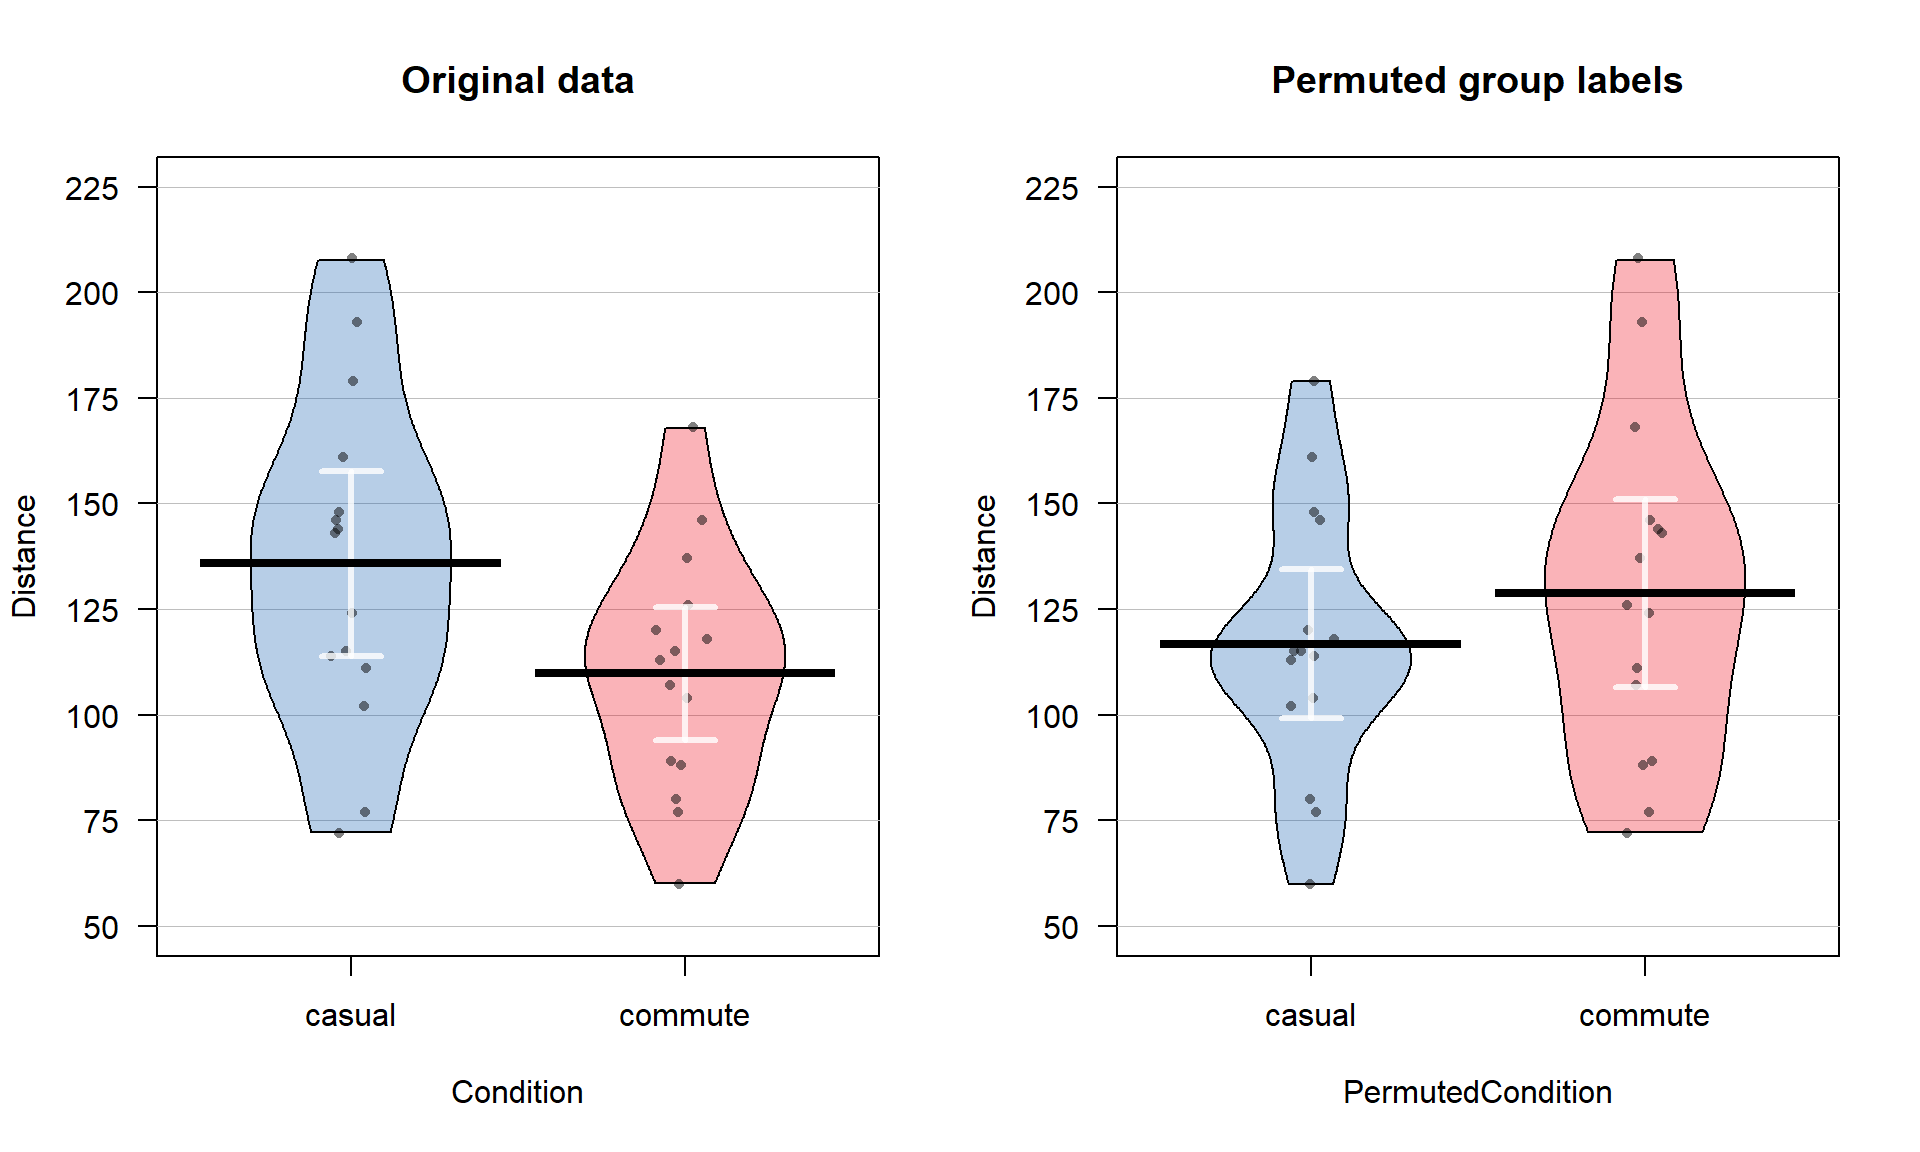
\includegraphics[width=0.75\linewidth]{02-linearmodelsreview_files/figure-latex/Figure2-7-1} 

}

\caption{Pirate-plots of Distance responses versus actual treatment groups and permuted groups. Note how the responses are the same but that they are shuffled between the two groups differently in the permuted data set. With the smaller sample size, the 95\% confidence intervals for each of the means are more clearly visible than with the original large data set.}\label{fig:Figure2-7}
\end{figure}

\indent The \texttt{diffmean} function is a simple way to get the differences in the means, but we can also start to learn about using the \texttt{lm} \index{\texttt{lm}} function -- that will be used for every chapter except for Chapter \ref{chapter5}. The \texttt{lm} stands for \textbf{\emph{linear model}} \index{linear model} and, as we will see moving forward, encompasses a wide array of different models and scenarios. The ability to estimate the difference in the mean of two groups is among its simplest uses.\footnote{This is a bit like getting a new convertible sports car and driving it to the grocery store -- there might be better ways to get groceries, but we probably would want to drive our new car as soon as we got it.} Notationally, it is very similar to other functions we have considered, \texttt{lm(y\ \textasciitilde{}\ x,\ data\ =\ ...)} where \texttt{y} is the response variable and \texttt{x} is the explanatory variable. Here that is \texttt{lm(Distance\ \textasciitilde{}\ Condition,\ data\ =\ dsample)} with \texttt{Condition} defined as a factor variable. With linear models, we will need to interrogate them to obtain a variety of useful information and our first ``interrogation'' function is usually the \texttt{summary} function. To use it, it is best to have stored the model into an object, something like \texttt{lm1}, and then we can apply the \texttt{summary()} \index{\texttt{summary}} function to the stored model object to get a suite of output:

\begin{Shaded}
\begin{Highlighting}[]
\NormalTok{lm1 }\OtherTok{\textless{}{-}} \FunctionTok{lm}\NormalTok{(Distance }\SpecialCharTok{\textasciitilde{}}\NormalTok{ Condition, }\AttributeTok{data =}\NormalTok{ dsample)}
\FunctionTok{summary}\NormalTok{(lm1)}
\end{Highlighting}
\end{Shaded}

\begin{verbatim}
## 
## Call:
## lm(formula = Distance ~ Condition, data = dsample)
## 
## Residuals:
##     Min      1Q  Median      3Q     Max 
## -63.800 -21.850   4.133  15.150  72.200 
## 
## Coefficients:
##                  Estimate Std. Error t value Pr(>|t|)
## (Intercept)       135.800      8.863  15.322 3.83e-15
## Conditioncommute  -25.933     12.534  -2.069   0.0479
## 
## Residual standard error: 34.33 on 28 degrees of freedom
## Multiple R-squared:  0.1326, Adjusted R-squared:  0.1016 
## F-statistic: 4.281 on 1 and 28 DF,  p-value: 0.04789
\end{verbatim}

This output is explored more in Chapter \ref{chapter3}, but for the moment, focus on the row labeled as \texttt{Conditioncommute} in the middle of the output. In the first (\texttt{Estimate}) column, there is -25.933. This is a number we saw before -- it is the difference in the sample means between \emph{commute} and \emph{casual} (\emph{commute} - \emph{casual}). When \texttt{lm} denotes a category in the row of the output (here \texttt{commute}), it is trying to indicate that the information to follow relates to the difference between this category and a baseline or reference category (here \texttt{casual}). The first (\texttt{(Intercept)}) row also contains a number we have seen before: -135.8 is the sample mean for the \emph{casual} group. So the \texttt{lm} is generating a coefficient for the mean of one of the groups and another as the difference in the two groups\footnote{This will be formalized and explained more in the next chapter when we encounter more than two groups in these same models. For now, it is recommended to start with the sample means from \texttt{favstats} for the two groups and then use that to sort out which direction the differencing was done in the \texttt{lm} output.}. In developing a test to assess evidence against the null hypothesis, we will focus on the difference in the sample means. So we want to be able to extract that number from this large suite of information. It ends up that we can apply the \texttt{coef} \index{\texttt{coef}} function to \texttt{lm} models and then access that second coefficient using the bracket notation. Specifically:

\begin{Shaded}
\begin{Highlighting}[]
\FunctionTok{coef}\NormalTok{(lm1)[}\DecValTok{2}\NormalTok{]}
\end{Highlighting}
\end{Shaded}

\begin{verbatim}
## Conditioncommute 
##        -25.93333
\end{verbatim}

This is the same result as using the \texttt{diffmean} function, so either could be used here. The estimated difference in the sample means in the permuted data set of 12.07 cm is available with:

\begin{Shaded}
\begin{Highlighting}[]
\NormalTok{lmP }\OtherTok{\textless{}{-}} \FunctionTok{lm}\NormalTok{(Distance }\SpecialCharTok{\textasciitilde{}}\NormalTok{ PermutedCondition, }\AttributeTok{data =}\NormalTok{ Perm1)}
\FunctionTok{coef}\NormalTok{(lmP)[}\DecValTok{2}\NormalTok{]}
\end{Highlighting}
\end{Shaded}

\begin{verbatim}
## PermutedConditioncommute 
##                 12.06667
\end{verbatim}

\indent Comparing the pirate-plots and the estimated difference in the sample means suggests that the observed difference was larger than what we got
when we did a single permutation. \index{permutation} Conceptually, permuting observations between group labels is
consistent with the null hypothesis -- this is a technique to generate results
that we might have gotten if the null hypothesis were true since the true models for the responses
are the same in the two groups if the null is true. We just need to repeat the
permutation process many times and track how unusual our observed result is
relative to this distribution of potential responses if the null were true.
If the observed differences are unusual relative to the results under
permutations, then there is evidence against the null hypothesis, and we can conclude,
in the direction of the alternative hypothesis, that the
true means differ. If the observed differences are similar to (or at least not
unusual relative to) what we get under random shuffling under the null model,
we would have a tough time concluding that there is any real difference between
the groups based on our observed data set. This is formalized using the \textbf{\emph{p-value}} as a measure of the strength of evidence against the null hypothesis and how we use it.

\hypertarget{section2-4}{%
\section{Permutation testing for the two sample mean situation}\label{section2-4}}

In any testing situation, you must define some function of the observations that
gives us a single number that addresses our question of interest. This quantity
is called a \textbf{\emph{test statistic}}. These often take on complicated forms and
have names like \(t\) or \(z\) statistics that relate to their parametric
\index{parametric}
(named)
distributions so we know where to look up
\textbf{\emph{p-values}}\footnote{P-values \index{p-value} are the
  probability of obtaining a result as extreme as or more extreme than we observed
  given that the null hypothesis is true.}. In randomization settings, they can
have simpler forms because we use the data set to find the
distribution of the statistic under the null hypothesis and don't need to rely on a
named distribution. We will label our test statistic \textbf{\emph{T}}
(for \textbf{T}est statistic) unless the test statistic has a commonly
used name. Since we are interested in comparing the means of the two groups, we
can define

\[T = \bar{x}_\text{commute} - \bar{x}_\text{casual},\]

which coincidentally is what the \texttt{diffmean} function and the second coefficient from the \texttt{lm} provided us previously.
We label our \textbf{\emph{observed test statistic}} (the one from the original data
set) as

\[T_{obs} = \bar{x}_\text{commute} - \bar{x}_\text{casual},\]

which happened to be -25.933 cm here. We will compare this result to the results
for the test statistic that we obtain from permuting the group labels. To
denote permuted results, we will add an * to the labels:

\[T^* = \bar{x}_{\text{commute}^*}-\bar{x}_{\text{casual}^*}.\]

We then compare the \(T_{obs} = \bar{x}_\text{commute} - \bar{x}_\text{casual} = -25.933\)
to the distribution of results that are possible for the permuted results (\(T^*\))
which corresponds to assuming the null hypothesis is true.

\indent We need to consider lots of permutations to do a permutation test.
\index{permutation!test}
In contrast to
your introductory statistics course where, if you did this, it was just a click
away, we are going to learn what was going on ``under the hood'' of the software you were using. Specifically, we
need a \textbf{\emph{for loop}} \index{\texttt{for loop}} in R to be able to repeatedly generate the permuted data
sets and record \(T^*\) for each one. Loops are a basic programming task that make
randomization methods possible as well as potentially simplifying any repetitive
computing task. To write a ``for loop'', we need to choose how many times we want
to do the loop (call that \texttt{B}) and decide on a counter to keep track of where
we are at in the loops (call that \texttt{b}, which goes from 1 up to \texttt{B}). The
simplest loop just involves printing out the index, \texttt{print(b)} at each step.
This is our first use of curly braces, \{ and \}, that are used to group the code
we want to repeatedly run as we proceed through the loop. By typing the following
code in a code chunk and then highlighting it all and hitting the run button,
R will go through the loop \emph{B} = 5 times, printing out the counter:

\begin{verbatim}
B <- 5
for (b in (1:B)){
  print(b)
}
\end{verbatim}

Note that when you highlight and run the code, it will look about the same with
``+'' printed after the first line to indicate that all the code is connected when
it appears in the console, looking like this:

\begin{Shaded}
\begin{Highlighting}[]
\SpecialCharTok{\textgreater{}} \ControlFlowTok{for}\NormalTok{(b }\ControlFlowTok{in}\NormalTok{ (}\DecValTok{1}\SpecialCharTok{:}\NormalTok{B))\{}
\SpecialCharTok{+}   \FunctionTok{print}\NormalTok{(b)}
\SpecialCharTok{+}\NormalTok{ \}}
\end{Highlighting}
\end{Shaded}

When you run these three lines of code (or compile a .Rmd file that contains this), the console will show you the following
output:

\begin{Shaded}
\begin{Highlighting}[]
\NormalTok{[}\DecValTok{1}\NormalTok{] }\DecValTok{1}
\NormalTok{[}\DecValTok{1}\NormalTok{] }\DecValTok{2}
\NormalTok{[}\DecValTok{1}\NormalTok{] }\DecValTok{3}
\NormalTok{[}\DecValTok{1}\NormalTok{] }\DecValTok{4}
\NormalTok{[}\DecValTok{1}\NormalTok{] }\DecValTok{5}
\end{Highlighting}
\end{Shaded}

\indent Instead of printing the counter, we want to use the loop to repeatedly compute
our test statistic across \emph{B} random permutations of the observations. The
\texttt{shuffle} function performs permutations of the group labels relative to
responses and the \texttt{coef(lmP){[}2{]}} extracts the estimated difference in the two group means in the permuted
data set. For a single permutation, the combination of shuffling \texttt{Condition} and
finding the difference in the means, storing it in a variable called \texttt{Ts} is:

\newpage

\begin{Shaded}
\begin{Highlighting}[]
\NormalTok{lmP }\OtherTok{\textless{}{-}} \FunctionTok{lm}\NormalTok{(Distance }\SpecialCharTok{\textasciitilde{}} \FunctionTok{shuffle}\NormalTok{(Condition), }\AttributeTok{data =}\NormalTok{ dsample)}
\NormalTok{Ts }\OtherTok{\textless{}{-}} \FunctionTok{coef}\NormalTok{(lmP)[}\DecValTok{2}\NormalTok{]}
\NormalTok{Ts}
\end{Highlighting}
\end{Shaded}

\begin{verbatim}
## shuffle(Condition)commute 
##               -0.06666667
\end{verbatim}

And putting this inside the \texttt{print} function allows us to find the test
statistic under 5 different permutations easily:

\begin{Shaded}
\begin{Highlighting}[]
\NormalTok{B }\OtherTok{\textless{}{-}} \DecValTok{5}
\ControlFlowTok{for}\NormalTok{ (b }\ControlFlowTok{in}\NormalTok{ (}\DecValTok{1}\SpecialCharTok{:}\NormalTok{B))\{}
\NormalTok{  lmP }\OtherTok{\textless{}{-}} \FunctionTok{lm}\NormalTok{(Distance }\SpecialCharTok{\textasciitilde{}} \FunctionTok{shuffle}\NormalTok{(Condition), }\AttributeTok{data =}\NormalTok{ dsample)}
\NormalTok{  Ts }\OtherTok{\textless{}{-}} \FunctionTok{coef}\NormalTok{(lmP)[}\DecValTok{2}\NormalTok{]}
  \FunctionTok{print}\NormalTok{(Ts)}
\NormalTok{\}}
\end{Highlighting}
\end{Shaded}

\begin{verbatim}
## shuffle(Condition)commute 
##                      -1.4 
## shuffle(Condition)commute 
##                  1.133333 
## shuffle(Condition)commute 
##                  20.86667 
## shuffle(Condition)commute 
##                  3.133333 
## shuffle(Condition)commute 
##                 -2.333333
\end{verbatim}

Finally, we would like to store the values of the test statistic instead of
just printing them out on each pass through the loop. To do this, we need to
create a variable to store the results, let's call it \texttt{Tstar}. We know that
we need to store \texttt{B} results so will create a vector\footnote{In statistics, vectors are one dimensional lists of numeric elements -- basically a column from a matrix of our tibble.} of length \emph{B}, which
contains \emph{B} elements, full of missing values (NA) using the \texttt{matrix} \index{texttt{matrix}} function with the \texttt{nrow} option specifying the number of elements:

\begin{Shaded}
\begin{Highlighting}[]
\NormalTok{Tstar }\OtherTok{\textless{}{-}} \FunctionTok{matrix}\NormalTok{(}\ConstantTok{NA}\NormalTok{, }\AttributeTok{nrow =}\NormalTok{ B)}
\NormalTok{Tstar}
\end{Highlighting}
\end{Shaded}

\begin{verbatim}
##      [,1]
## [1,]   NA
## [2,]   NA
## [3,]   NA
## [4,]   NA
## [5,]   NA
\end{verbatim}

Now we can run our loop \emph{B} times and store the results in \texttt{Tstar}.

\begin{Shaded}
\begin{Highlighting}[]
\ControlFlowTok{for}\NormalTok{ (b }\ControlFlowTok{in}\NormalTok{ (}\DecValTok{1}\SpecialCharTok{:}\NormalTok{B))\{}
\NormalTok{  lmP }\OtherTok{\textless{}{-}} \FunctionTok{lm}\NormalTok{(Distance }\SpecialCharTok{\textasciitilde{}} \FunctionTok{shuffle}\NormalTok{(Condition), }\AttributeTok{data =}\NormalTok{ dsample)}
\NormalTok{  Tstar[b] }\OtherTok{\textless{}{-}} \FunctionTok{coef}\NormalTok{(lmP)[}\DecValTok{2}\NormalTok{]}
\NormalTok{\}}
\CommentTok{\# Print out the results stored in Tstar with the next line of code}
\end{Highlighting}
\end{Shaded}

\newpage

\begin{Shaded}
\begin{Highlighting}[]
\NormalTok{Tstar}
\end{Highlighting}
\end{Shaded}

\begin{verbatim}
##           [,1]
## [1,] -5.400000
## [2,] -3.266667
## [3,] -7.933333
## [4,] 13.133333
## [5,] -6.466667
\end{verbatim}

\indent Five permutations are still not enough to assess whether our \(T_{obs}\)
of -25.933 is unusual and we need to do many permutations to get an accurate
assessment of the possibilities under the null hypothesis.
\index{permutation!test}
It is common practice
to consider something like 1,000 permutations. The \texttt{Tstar} vector when we set
\emph{B} to be large, say \texttt{B\ =\ 1000}, contains the permutation distribution \index{permutation!distribution} for the
selected test statistic under\footnote{We often say
  ``under'' in statistics and we mean ``given that the following is true''.} the null
hypothesis -- what is called the \textbf{\emph{null distribution}} of the statistic. The
null distribution is the distribution of possible values of a statistic
under the null hypothesis. We want to visualize this distribution and use it to
assess how unusual our \(T_{obs}\) result of -25.933 cm was relative to all the
possibilities under permutations (under the null hypothesis). So we repeat the
loop, now with \(B = 1000\) and generate a histogram (modified to add counts to the bars using \texttt{stat\_bin}\footnote{This is another place where the code is a bit cryptic when you are starting -- just copy this entire chunk of code -- you only ever need to modify the \texttt{lm} line in this code!}), density curve, and summary
statistics of the results:



\begin{figure}[ht!]

{\centering 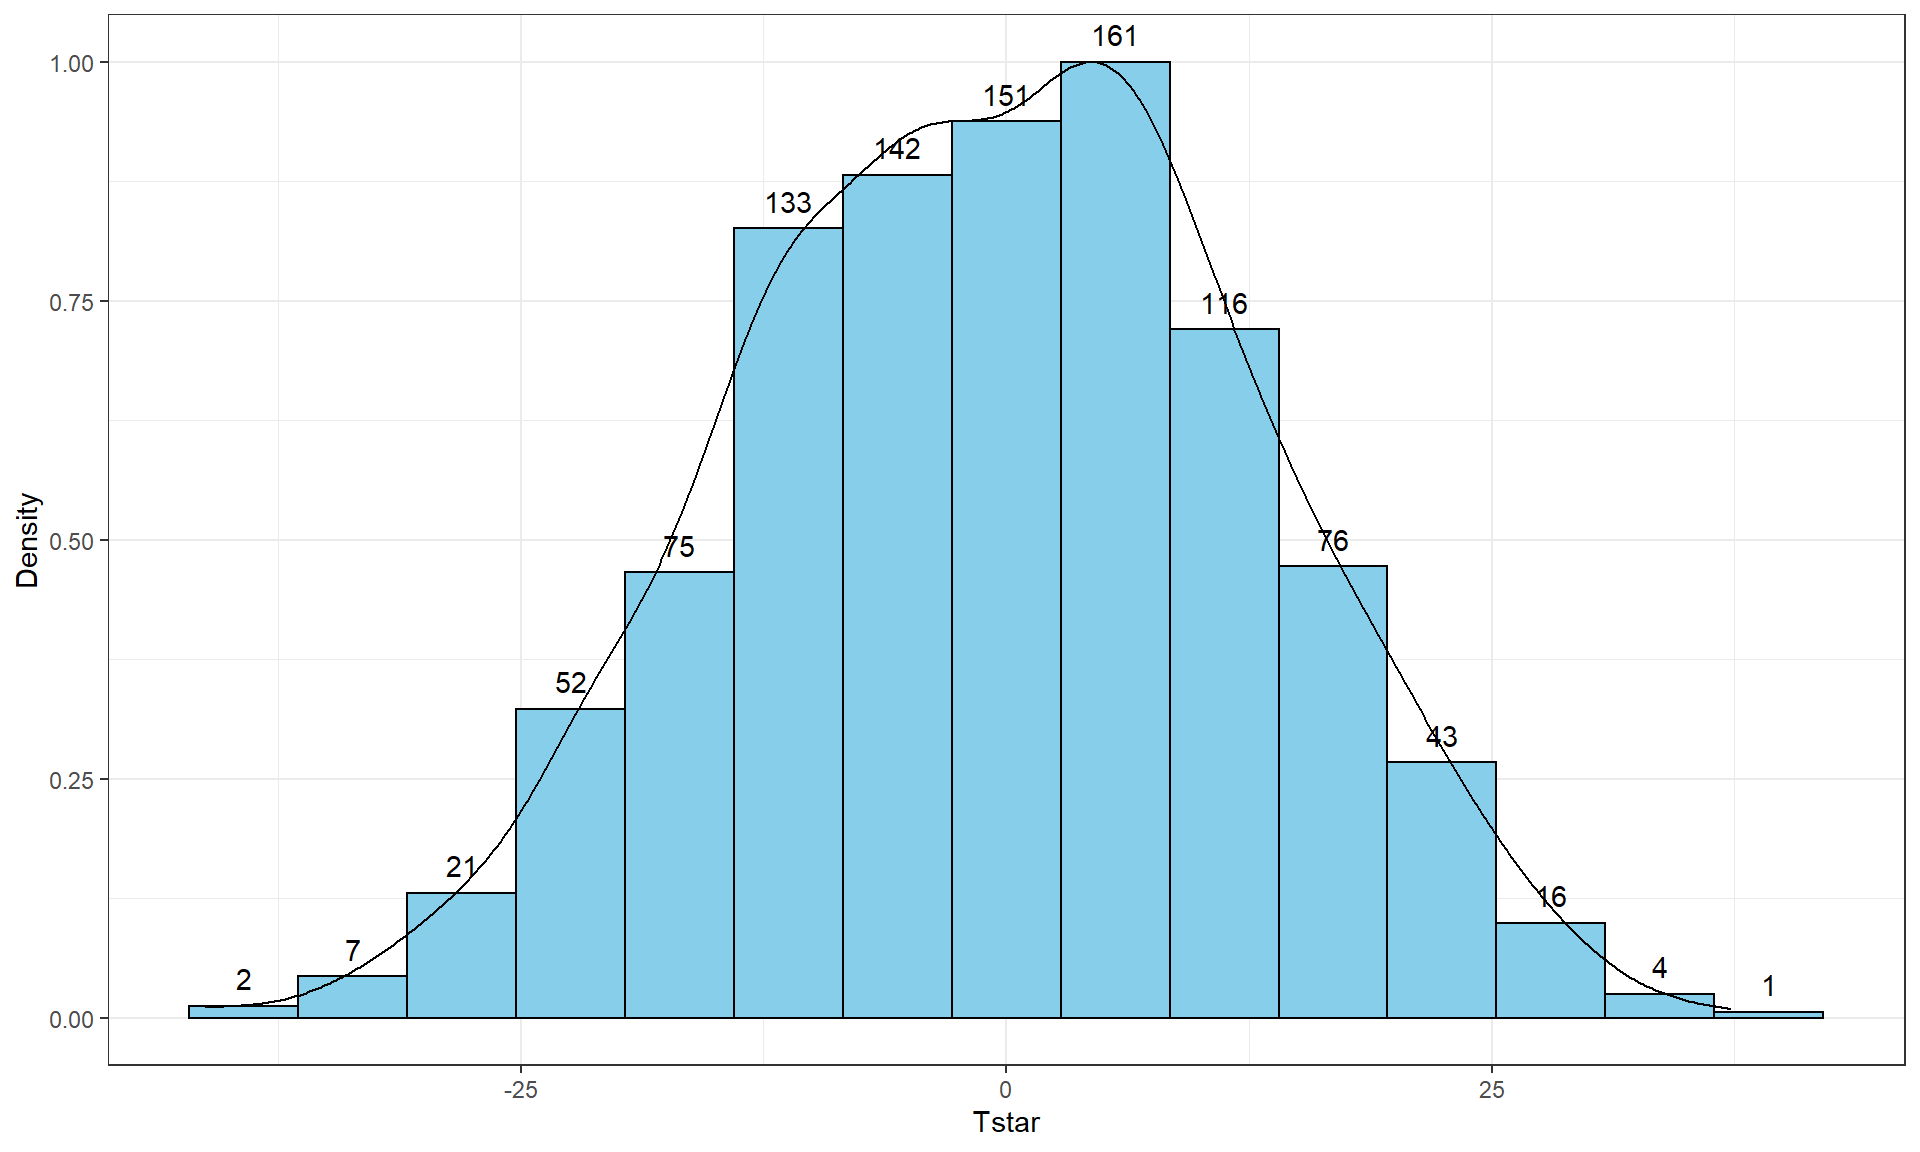
\includegraphics[width=0.75\linewidth]{02-linearmodelsreview_files/figure-latex/Figure2-8-1} 

}

\caption{Histogram (left, with counts in bars) and density curve (right) of values of test statistic for \emph{B} = 1,000 permutations.}\label{fig:Figure2-8}
\end{figure}

\begin{Shaded}
\begin{Highlighting}[]
\NormalTok{B }\OtherTok{\textless{}{-}} \DecValTok{1000}
\NormalTok{Tstar }\OtherTok{\textless{}{-}} \FunctionTok{matrix}\NormalTok{(}\ConstantTok{NA}\NormalTok{, }\AttributeTok{nrow =}\NormalTok{ B)}
\ControlFlowTok{for}\NormalTok{ (b }\ControlFlowTok{in}\NormalTok{ (}\DecValTok{1}\SpecialCharTok{:}\NormalTok{B))\{}
\NormalTok{  lmP }\OtherTok{\textless{}{-}} \FunctionTok{lm}\NormalTok{(Distance }\SpecialCharTok{\textasciitilde{}} \FunctionTok{shuffle}\NormalTok{(Condition), }\AttributeTok{data =}\NormalTok{ dsample)}
\NormalTok{  Tstar[b] }\OtherTok{\textless{}{-}} \FunctionTok{coef}\NormalTok{(lmP)[}\DecValTok{2}\NormalTok{]}
\NormalTok{\}}
\end{Highlighting}
\end{Shaded}

\newpage

\small

\begin{Shaded}
\begin{Highlighting}[]
\FunctionTok{tibble}\NormalTok{(Tstar) }\SpecialCharTok{\%\textgreater{}\%} \FunctionTok{ggplot}\NormalTok{(}\FunctionTok{aes}\NormalTok{(}\AttributeTok{x =}\NormalTok{ Tstar)) }\SpecialCharTok{+} 
  \FunctionTok{geom\_histogram}\NormalTok{(}\FunctionTok{aes}\NormalTok{(}\AttributeTok{y =}\NormalTok{ ..ncount..), }\AttributeTok{bins =} \DecValTok{15}\NormalTok{, }\AttributeTok{col =} \DecValTok{1}\NormalTok{, }\AttributeTok{fill =} \StringTok{"skyblue"}\NormalTok{, }\AttributeTok{center =} \DecValTok{0}\NormalTok{) }\SpecialCharTok{+} 
  \FunctionTok{geom\_density}\NormalTok{(}\FunctionTok{aes}\NormalTok{(}\AttributeTok{y =}\NormalTok{ ..scaled..)) }\SpecialCharTok{+}
  \FunctionTok{theme\_bw}\NormalTok{() }\SpecialCharTok{+}
  \FunctionTok{labs}\NormalTok{(}\AttributeTok{y =} \StringTok{"Density"}\NormalTok{) }\SpecialCharTok{+}
  \FunctionTok{stat\_bin}\NormalTok{(}\FunctionTok{aes}\NormalTok{(}\AttributeTok{y =}\NormalTok{ ..ncount.., }\AttributeTok{label =}\NormalTok{ ..count..), }\AttributeTok{bins =} \DecValTok{15}\NormalTok{, }\AttributeTok{geom =} \StringTok{"text"}\NormalTok{, }\AttributeTok{vjust =} \SpecialCharTok{{-}}\FloatTok{0.75}\NormalTok{)}

\FunctionTok{favstats}\NormalTok{(Tstar)}
\end{Highlighting}
\end{Shaded}

\begin{verbatim}
##        min        Q1     median  Q3      max       mean       sd    n missing
##  -41.26667 -10.06667 -0.3333333 8.6 37.26667 -0.5054667 13.17156 1000       0
\end{verbatim}

\normalsize

Figure \ref{fig:Figure2-8} contains visualizations of \(T^*\) and the \texttt{favstats}
summary provides the related numerical summaries. Our observed \(T_{obs}\)
of -25.933 seems somewhat unusual relative to these results with only
30 \(T^*\) values smaller than -25 based on the
histogram. We need to make more specific comparisons of the permuted results
versus our observed result to be able to clearly decide whether our observed
result is really unusual.

\indent To make the comparisons more concrete, first we can enhance the previous graphs
by adding the value of the test statistic from the real data set, as shown in
Figure \ref{fig:Figure2-9}, using the \texttt{geom\_vline} \index{\texttt{geom\_vline}} function to draw a vertical
line at our \(T_{obs}\) value specified in the \texttt{xintercept} option. Notice the
order of the parameters. The code for the vertical line is before the code for
the bin counts. This order is prefered so that the counts are still readable if
the vertical line and a bin count are in the same horizontal position.



\begin{figure}[ht!]

{\centering 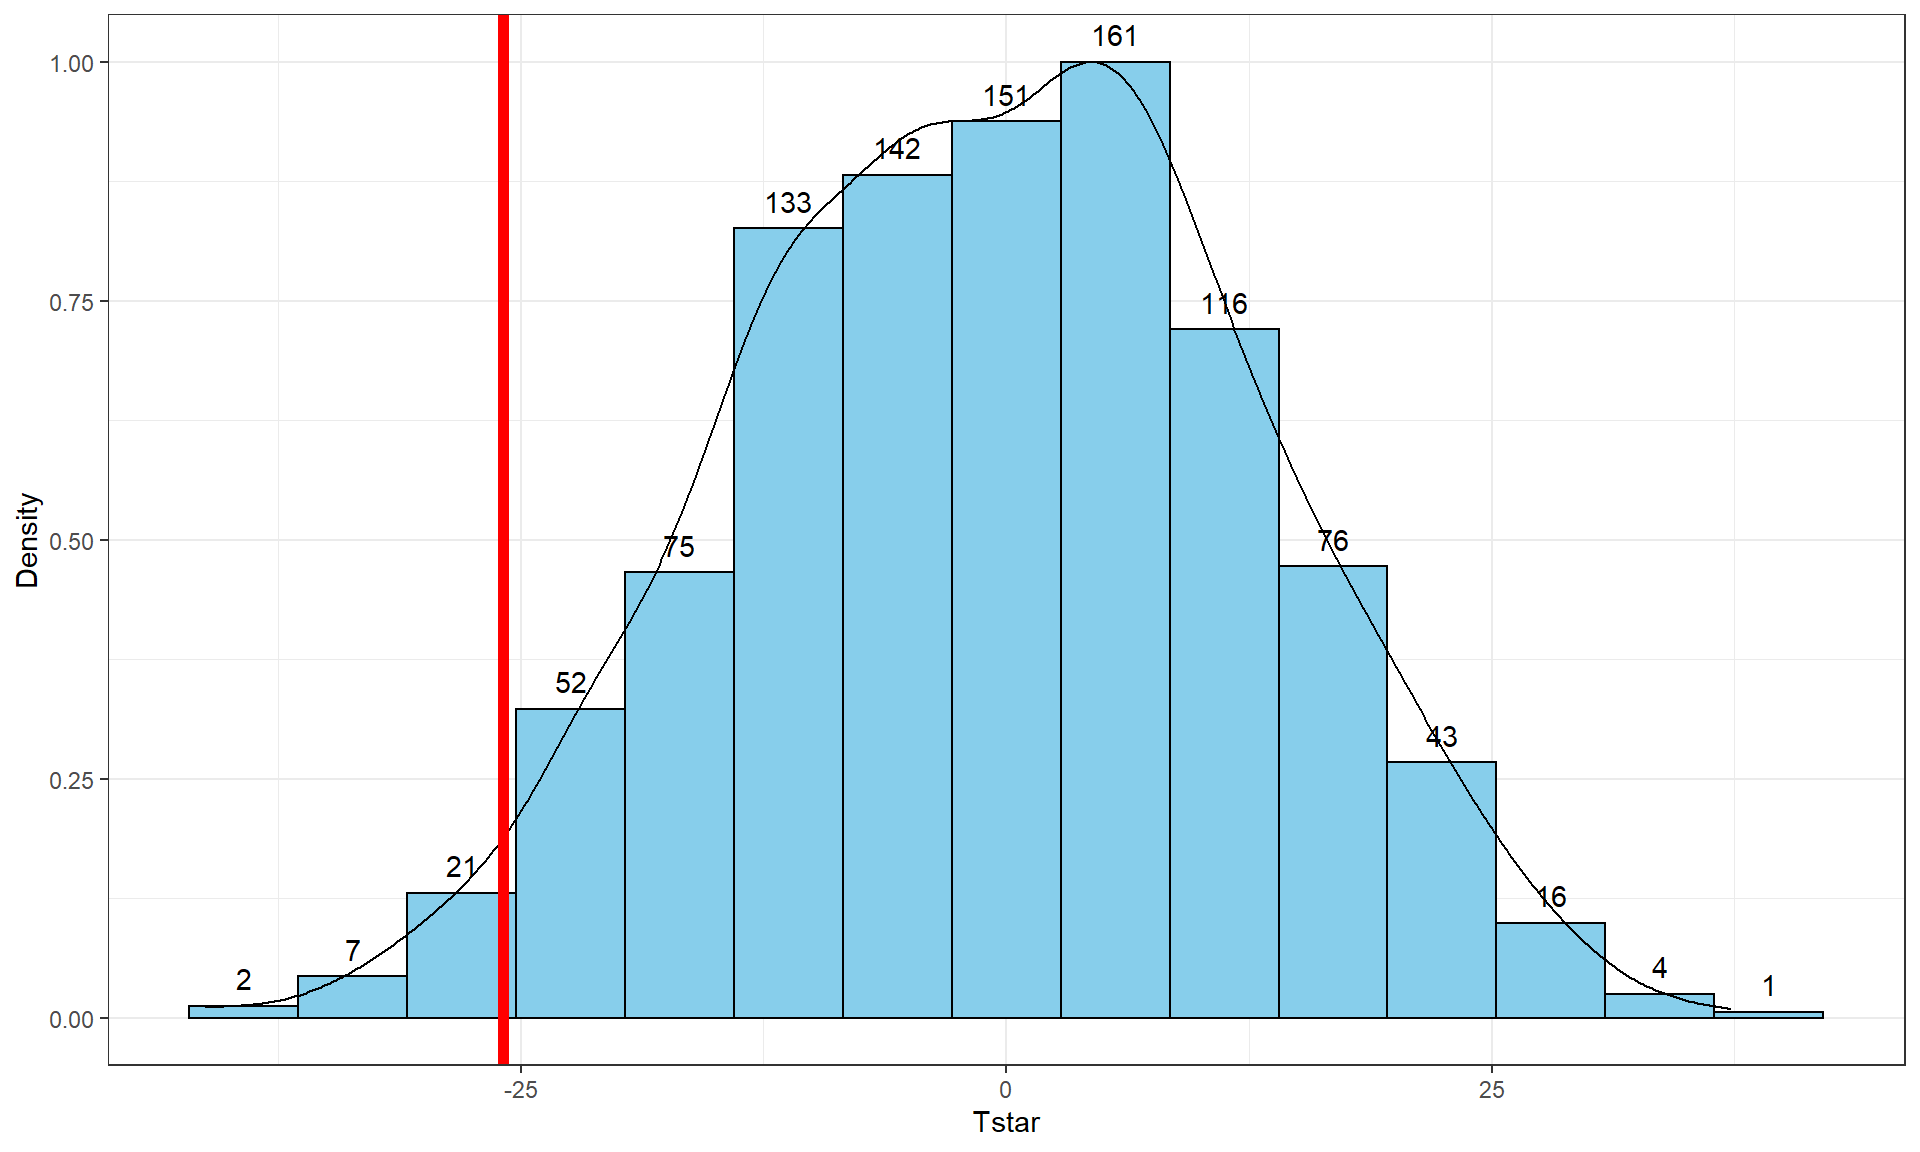
\includegraphics[width=0.75\linewidth]{02-linearmodelsreview_files/figure-latex/Figure2-9-1} 

}

\caption{Histogram and density curve of values of test statistic for 1,000 permutations with bold vertical line for the value of observed test statistic.}\label{fig:Figure2-9}
\end{figure}

\small

\begin{Shaded}
\begin{Highlighting}[]
\NormalTok{Tobs }\OtherTok{\textless{}{-}} \SpecialCharTok{{-}}\FloatTok{25.933}
\FunctionTok{tibble}\NormalTok{(Tstar) }\SpecialCharTok{\%\textgreater{}\%} \FunctionTok{ggplot}\NormalTok{(}\FunctionTok{aes}\NormalTok{(}\AttributeTok{x =}\NormalTok{ Tstar)) }\SpecialCharTok{+} 
  \FunctionTok{geom\_histogram}\NormalTok{(}\FunctionTok{aes}\NormalTok{(}\AttributeTok{y =}\NormalTok{ ..ncount..), }\AttributeTok{bins =} \DecValTok{15}\NormalTok{, }\AttributeTok{col =} \DecValTok{1}\NormalTok{, }\AttributeTok{fill =} \StringTok{"skyblue"}\NormalTok{, }\AttributeTok{center =} \DecValTok{0}\NormalTok{) }\SpecialCharTok{+} 
  \FunctionTok{geom\_density}\NormalTok{(}\FunctionTok{aes}\NormalTok{(}\AttributeTok{y =}\NormalTok{ ..scaled..)) }\SpecialCharTok{+}
  \FunctionTok{theme\_bw}\NormalTok{() }\SpecialCharTok{+}
  \FunctionTok{labs}\NormalTok{(}\AttributeTok{y =} \StringTok{"Density"}\NormalTok{) }\SpecialCharTok{+}
  \FunctionTok{geom\_vline}\NormalTok{(}\AttributeTok{xintercept =}\NormalTok{ Tobs, }\AttributeTok{col =} \StringTok{"red"}\NormalTok{, }\AttributeTok{lwd =} \DecValTok{2}\NormalTok{) }\SpecialCharTok{+}
  \FunctionTok{stat\_bin}\NormalTok{(}\FunctionTok{aes}\NormalTok{(}\AttributeTok{y =}\NormalTok{ ..ncount.., }\AttributeTok{label =}\NormalTok{ ..count..), }\AttributeTok{bins =} \DecValTok{15}\NormalTok{, }\AttributeTok{geom =} \StringTok{"text"}\NormalTok{, }\AttributeTok{vjust =} \SpecialCharTok{{-}}\FloatTok{0.75}\NormalTok{)}
\end{Highlighting}
\end{Shaded}

\normalsize

\newpage

Second, we can calculate the exact number of permuted results that were as
small or smaller
than what we observed. To calculate the proportion of the 1,000 values that were
as small or smaller than what we observed, we will use the \texttt{pdata} function.
\index{\texttt{pdata()}}
To use this
function, we need to provide the distribution of values to compare to the cut-off
(\texttt{Tstar}), the cut-off point (\texttt{Tobs}), and whether we want calculate the
proportion that are below (left of) or above (right of) the cut-off
(\texttt{lower.tail\ =\ T} option provides the proportion of values to the left of (below) the cutoff
of interest).

\begin{Shaded}
\begin{Highlighting}[]
\FunctionTok{pdata}\NormalTok{(Tstar, Tobs, }\AttributeTok{lower.tail =}\NormalTok{ T)[[}\DecValTok{1}\NormalTok{]]}
\end{Highlighting}
\end{Shaded}

\begin{verbatim}
## [1] 0.027
\end{verbatim}

The proportion of 0.027 tells us that 27 of the 1,000 permuted results
(2.7\%) were as small or smaller than what we observed. This type of
work is how we can
generate \textbf{\emph{p-values}} using permutation distributions.
\index{p-value!permutation distribution}
\index{permutation!distribution}
P-values,
\index{p-value}
as you should
remember, are the probability of getting a result as extreme as or more extreme
than what we observed, \(\underline{\text{given that the null is true}}\). Finding
only 27
permutations of 1,000 that were as small or smaller than our observed result suggests that it
is hard to find a result like what we observed if there really were no difference,
although it is not impossible.

\indent When testing hypotheses for two groups, there are two types of alternative
hypotheses, one-sided or two-sided. \textbf{\emph{One-sided tests}} involve only considering
differences in one-direction (like \(\mu_1 > \mu_2\)) and are performed when
researchers can decide \textbf{\emph{a priori}}\footnote{This is a fancy way of saying ``in advance'',
  here in advance of seeing the observations.} which group should have a larger mean
if there is going to be any sort of difference. In this situation, we did not
know enough about the potential impacts of the outfits to know which group should
be larger than the other so should do a two-sided test. It is important to
remember that you can't look at the responses to decide on the hypotheses. It is
often safer and more \textbf{\emph{conservative}}\footnote{Statistically, a conservative method is
  one that provides less chance of rejecting the null hypothesis in comparison to
  some other method or less than some pre-defined standard. A liberal method provides higher rates of false rejections.} \index{conservative} \index{liberal} to start with a
\textbf{\emph{two-sided alternative}} (\(\mathbf{H_A: \mu_1 \ne \mu_2}\)). To do a 2-sided
test, find the area smaller than what we observed as above (or larger if the test statistic had been positive). We also need to add
the area in the other tail (here the right tail) similar to what we observed in the
right tail. Some statisticians suggest doubling the area in one tail but we will collect
information on the number that were as or more extreme than the same
value in the other
tail\footnote{Both approaches are reasonable. By using both tails of the distribution we can incorporate potential differences in shape in both tails of the permutation distribution.}. In other words, we count the proportion below -25.933 and over 25.933. So
we need to find how many of the permuted results were larger than or equal
to 25.933 cm
to add to our previous proportion. Using \texttt{pdata} with \texttt{-Tobs} as the cut-off
and \texttt{lower.tail\ =\ F} provides this result:
\index{\texttt{pdata()}}

\begin{Shaded}
\begin{Highlighting}[]
\FunctionTok{pdata}\NormalTok{(Tstar, }\SpecialCharTok{{-}}\NormalTok{Tobs, }\AttributeTok{lower.tail =}\NormalTok{ F)[[}\DecValTok{1}\NormalTok{]]}
\end{Highlighting}
\end{Shaded}

\begin{verbatim}
## [1] 0.017
\end{verbatim}

So the p-value to test our null hypothesis of no difference in the true means
between the groups is 0.027 + 0.017, providing a p-value of 0.044.
Figure \ref{fig:Figure2-10} shows both cut-offs on the histogram and density curve.



\begin{figure}[ht!]

{\centering 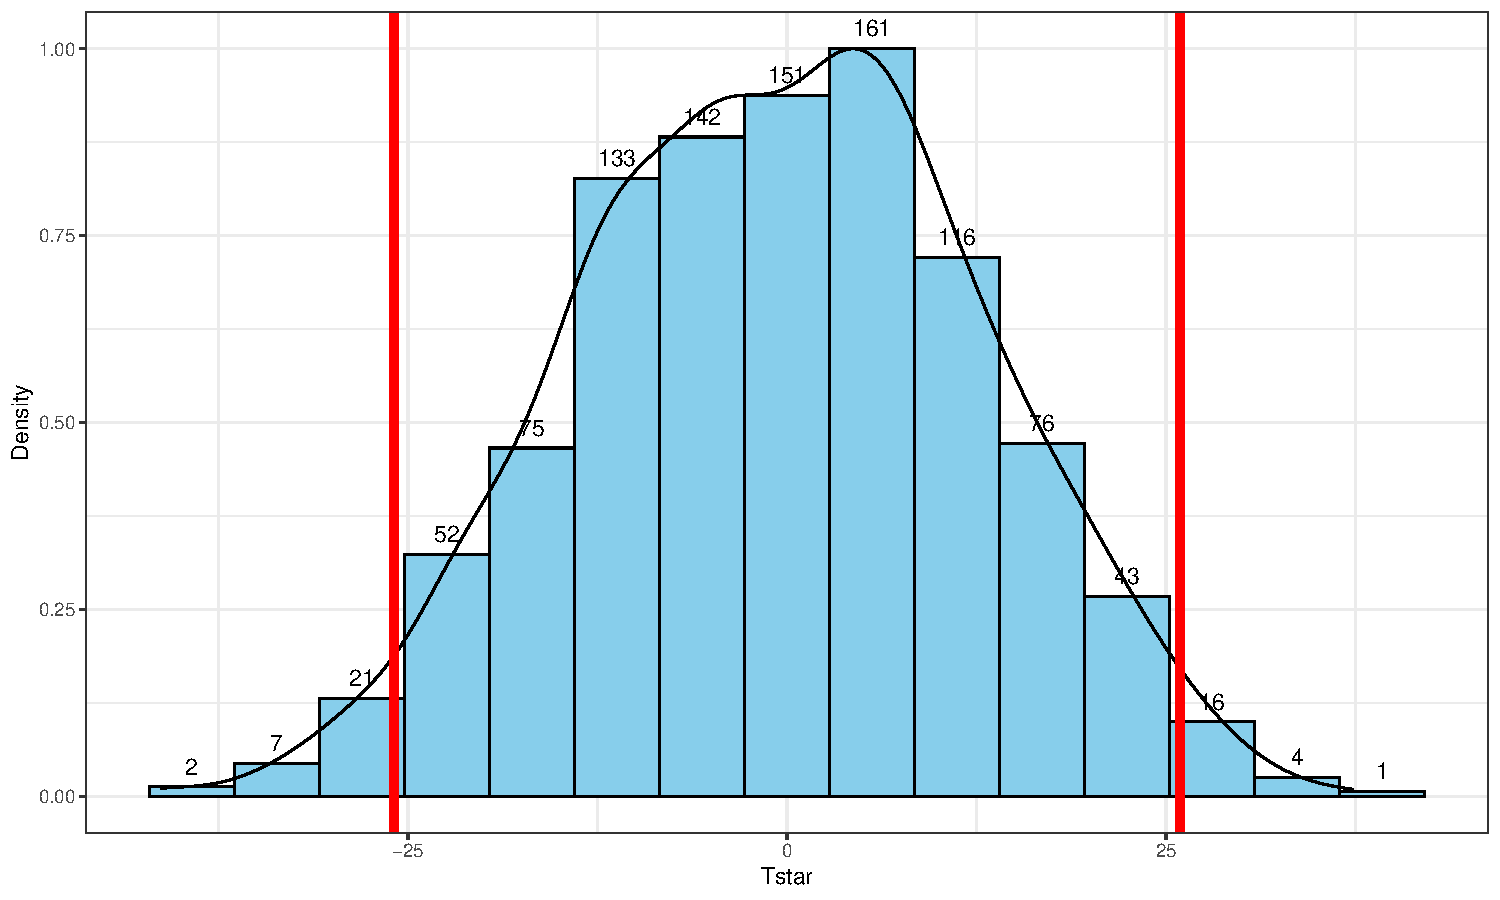
\includegraphics[width=0.75\linewidth]{02-linearmodelsreview_files/figure-latex/Figure2-10-1} 

}

\caption{Histogram and density curve of values of test statistic for 1,000 permutations with bold lines for value of observed test statistic (-25.933) and its opposite value (25.933) required for performing the two-sided test.}\label{fig:Figure2-10}
\end{figure}

\begin{Shaded}
\begin{Highlighting}[]
\FunctionTok{tibble}\NormalTok{(Tstar) }\SpecialCharTok{\%\textgreater{}\%} \FunctionTok{ggplot}\NormalTok{(}\FunctionTok{aes}\NormalTok{(}\AttributeTok{x =}\NormalTok{ Tstar)) }\SpecialCharTok{+} 
  \FunctionTok{geom\_histogram}\NormalTok{(}\FunctionTok{aes}\NormalTok{(}\AttributeTok{y =}\NormalTok{ ..ncount..), }\AttributeTok{bins =} \DecValTok{15}\NormalTok{, }\AttributeTok{col =} \DecValTok{1}\NormalTok{, }\AttributeTok{fill =} \StringTok{"skyblue"}\NormalTok{, }\AttributeTok{center =} \DecValTok{0}\NormalTok{) }\SpecialCharTok{+} 
  \FunctionTok{geom\_density}\NormalTok{(}\FunctionTok{aes}\NormalTok{(}\AttributeTok{y =}\NormalTok{ ..scaled..)) }\SpecialCharTok{+}
  \FunctionTok{theme\_bw}\NormalTok{() }\SpecialCharTok{+}
  \FunctionTok{labs}\NormalTok{(}\AttributeTok{y =} \StringTok{"Density"}\NormalTok{) }\SpecialCharTok{+}
  \FunctionTok{geom\_vline}\NormalTok{(}\AttributeTok{xintercept =} \FunctionTok{c}\NormalTok{(}\SpecialCharTok{{-}}\DecValTok{1}\NormalTok{,}\DecValTok{1}\NormalTok{)}\SpecialCharTok{*}\NormalTok{Tobs, }\AttributeTok{col =} \StringTok{"red"}\NormalTok{, }\AttributeTok{lwd =} \DecValTok{2}\NormalTok{) }\SpecialCharTok{+}
  \FunctionTok{stat\_bin}\NormalTok{(}\FunctionTok{aes}\NormalTok{(}\AttributeTok{y =}\NormalTok{ ..ncount.., }\AttributeTok{label =}\NormalTok{ ..count..), }\AttributeTok{bins =} \DecValTok{15}\NormalTok{, }
           \AttributeTok{geom =} \StringTok{"text"}\NormalTok{, }\AttributeTok{vjust =} \SpecialCharTok{{-}}\FloatTok{0.75}\NormalTok{)}
\end{Highlighting}
\end{Shaded}

\indent In general, the \textbf{\emph{one-sided test p-value}}
\index{p-value!one-sided test}
is the proportion of the
permuted results that are as extreme or more extreme than observed in the
direction of the \emph{alternative}
hypothesis (lower or upper tail, remembering that this also depends on the
direction of the difference taken). For the two-sided test, the p-value
\index{p-value!two-sided test}
is the
proportion of the permuted results that are \emph{less than or equal to the negative
version of the observed statistic and greater than or equal to the positive
version of the observed statistic}. Using absolute
values (\textbar{} \textbar), we can simplify this: the \textbf{\emph{two-sided p-value}} is the
\emph{proportion of the \textbar permuted statistics\textbar{} that are as large or larger than
\textbar observed statistic\textbar{}}.
This will always work and finds areas in both tails regardless of whether the
observed statistic is positive or negative. In R, the \texttt{abs} function \index{\texttt{abs}} provides the
\textbf{\emph{absolute value}} and we can again use \texttt{pdata} to find our p-value in one line
of code:
\index{\texttt{pdata()}}

\begin{Shaded}
\begin{Highlighting}[]
\FunctionTok{pdata}\NormalTok{(}\FunctionTok{abs}\NormalTok{(Tstar), }\FunctionTok{abs}\NormalTok{(Tobs), }\AttributeTok{lower.tail =}\NormalTok{ F)[[}\DecValTok{1}\NormalTok{]]}
\end{Highlighting}
\end{Shaded}

\begin{verbatim}
## [1] 0.044
\end{verbatim}

We will encourage you to think through what might constitute strong evidence
against your null hypotheses and then discuss how strong you feel the evidence
is against the null hypothesis in the p-value that you obtained. Basically,
p-values present a measure of evidence against the null hypothesis,
\index{p-value}
with smaller
values presenting more evidence against the null. They range from 0 to 1 and you
should interpret them on a graded scale from strong evidence (close to 0) to little evidence to no
evidence (1). We will discuss the use of a fixed \textbf{\emph{significance level}}
below as it is still commonly used in many fields and is necessary to discuss to think
about the theory of hypothesis testing, but, for the moment,
we can say that there is moderate evidence against the null hypothesis
presented by having a p-value of 0.044 because our observed result is somewhat
rare relative to what we would expect if the null hypothesis was true. And so
we might conclude (in the direction
of the alternative) that there is a difference in the population means in the
two groups, but that depends on what you think about how unusual that result was. It is also reasonable to feel that this is not sufficient evidence to conclude that there is a difference in the true means even though many people feel that p-values less than 0.05 are fairly strong evidence against the null hypothesis. If you do not rate this as strong enough evidence (or in general obtain weak evidence) to conclude that there is a difference, then you can only say that there might not be a difference in the means. We can't conclude that the null hypothesis is true -- we just failed to find enough evidence to be sure that it is wrong. It might still be wrong but we couldn't detect it, either as a mistake because of an unusual sample from our population, or because our sample size was not large enough to detect the size of difference in the populations, or results with larger p-values could happen because there really isn't a difference. We don't know which of these might be the truth and certainly don't know that the null hypothesis is true even if the p-value obtained is 1\footnote{P-values of 1 are the only result that provide no evidence against the null hypothesis but this still doesn't prove that the null hypothesis is true.}.

\indent Before we move on, let's note some interesting features of the permutation
distribution of the difference in the sample means shown in
Figure \ref{fig:Figure2-10}. \index{permutation!distribution}

\begin{enumerate}
\def\labelenumi{\arabic{enumi}.}
\item
  It is basically centered at 0. Since we are performing permutations assuming
  the null model is true, we are assuming that \(\mu_1 = \mu_2\) which implies that
  \(\mu_1 - \mu_2 = 0\). This also suggests that 0 should be the center of the
  permutation distribution and it was.
\item
  It is approximately normally distributed. This is due to the \textbf{\emph{Central Limit Theorem}}\footnote{We'll leave the discussion of the CLT to your previous statistics coursework
    or an internet search. For this material, just remember that it has something to do with distributions of statistics
    looking more normal as the sample size increases.}, where the
  \textbf{\emph{sampling distribution}} (distribution of all possible results for samples
  of this size) of the difference in sample means (\(\bar{x}_1 - \bar{x}_2\)) becomes
  more normally distributed as the sample sizes increase. With 15
  observations in each group, we have no guarantee to have a relatively normal looking
  distribution of the difference in the sample means but with the distributions of the original observations looking somewhat normally distributed, the sampling distribution of the sample means likely will look fairly normal. This result will allow us to
  use a parametric
  \index{parametric}
  method to approximate this sampling distribution under the null
  model if some assumptions are met, as we'll discuss below.
\item
  Our observed difference in the sample means (-25.933) is a fairly unusual
  result relative to the rest of these results but there are some permuted data
  sets that produce more extreme differences in the sample means. When the
  observed differences are really large, we may not see any permuted results
  that are as extreme as what we observed. When \texttt{pdata} gives you 0, the p-value
  \index{p-value!zero}
  should be reported to be smaller than 0.001 (\textbf{not 0!}) if \emph{B} is 1,000 since it happened
  in less than 1 in 1,000 tries but does occur once -- in the actual data set. This applies to any p-values when they are very small -- just report them as less than 0.001, or 0.0001 if you prefer that next smaller upper limit, when they are under these values.
\item
  Since our null model is not specific about the direction of the difference,
  considering a result like ours but in the other direction (25.933 cm) needs to
  be included. The observed result seems to put about the same area in both tails
  of the distribution but it is not exactly the same. The small difference in the
  tails is a useful aspect of this approach compared to the parametric method
  discussed below as it accounts for potential asymmetry in the sampling distribution.
\end{enumerate}

\indent Earlier, we decided that the p-value provided moderate evidence against
the null hypothesis. You should use your own judgment about whether the p-value obtain is sufficiently small to conclude that you think the null hypothesis is wrong. Remembering
that the p-value is the probability
\index{p-value}
you would observe a result like you did (or more extreme), assuming the null
hypothesis is true; this tells you that the smaller the p-value is, the more
evidence you have against the null. Figure \ref{fig:Figure2-11} provides a
diagram of some suggestions for the graded p-value interpretation that you can
use. The next section provides a more formal
review of the hypothesis testing
\index{hypothesis testing}
infrastructure, terminology, and some of
things that can happen when testing hypotheses. P-values have been (validly)
\index{p-value!criticism}
criticized for the inability of studies to be reproduced, for the bias in
publications to only include studies that have small p-values, and for the lack of
thought that often accompanies using a fixed significance level to make decisions (and only focusing on that decision). To alleviate
some of these criticisms, we recommend reporting the strength of evidence of the
result based on the p-value and also reporting and discussing the size of the
estimated results (with a measure of precision of the estimated difference). We will explore the implications of how p-values are used in scientific research in Section \ref{section2-8}.



\begin{figure}[ht!]

{\centering 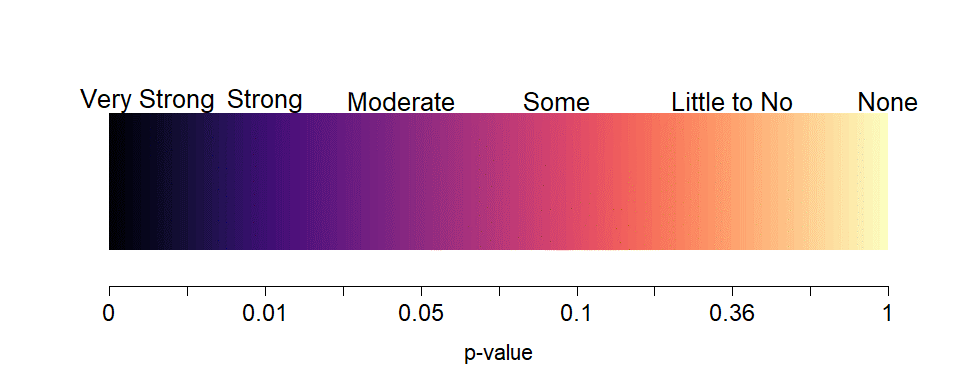
\includegraphics[width=1\linewidth]{chapter2_files/pvalueStrengths} 

}

\caption{Graphic suggesting potential interpretations of strength of evidence based on gradient of p-values. P-values range from 0 to 1, with only a p-value of 1.0 providing no evidence against the null hypothesis.}\label{fig:Figure2-11}
\end{figure}

\newpage

\hypertarget{section2-5}{%
\section{Hypothesis testing (general)}\label{section2-5}}

In hypothesis testing
\index{hypothesis testing}
(sometimes more explicitly called ``Null Hypothesis
Significance Testing'' or NHST), it is formulated to answer a specific question about
a population or true parameter(s) using a statistic based on a data set.
In your previous statistics course, you (hopefully) considered one-sample
hypotheses about population means and proportions and the two-sample mean
situation we are focused on here. Hypotheses relate to trying to answer
the question about whether the population mean overtake distances between the two
groups are different, with an initial assumption of no difference.

\indent NHST is much like a criminal trial with a jury where you are in the role
of a jury member. Initially, the defendant
is assumed innocent. In our situation, the true means are assumed to be
equal between the groups. Then evidence is presented and, as a juror,
you analyze it. In statistical hypothesis testing,
\index{hypothesis testing}
data are collected and
analyzed. Then you have to decide if we had ``enough'' evidence to reject
the initial assumption (``innocence'' that is initially assumed). To make
this decision, you want to have thought about and decided on the standard of
evidence required to reject the initial assumption. In criminal cases,
``beyond a reasonable doubt'' is used. Wikipedia's definition
(\url{https://en.wikipedia.org/wiki/Reasonable_doubt}) suggests that this
standard is that ``there can still be a doubt, but only to the extent
that it would not affect a reasonable person's belief regarding whether
or not the defendant is guilty''. In civil trials, a lower standard called
a ``preponderance of evidence'' is used. Based on that defined and pre-decided
(\emph{a priori}) measure, you decide that the defendant is guilty or not guilty.
In statistics, the standard is set by choosing a significance level, \(\alpha\), and then you compare the p-value
\index{p-value}
to it. In this approach, if the p-value is less than
\(\alpha\), we reject the null hypothesis. The choice of the significance level
is like the variation in standards of evidence between criminal and civil
trials -- and in all situations everyone should know the standards required
for rejecting the initial assumption before any information is ``analyzed''.
Once someone is found guilty, then there is the matter of sentencing which
is related to the impacts (``size'') of the crime. In statistics, this is
similar to the estimated size of differences and the related judgments
about whether the differences are practically important or not. If the
crime is proven beyond a reasonable doubt but it is a minor crime, then
the sentence will be small. With the same level of evidence and a more
serious crime, the sentence will be more dramatic. This latter step is more critical than the p-value as it directly relates to actions to be taken based on the research but unfortunately p-values and the related decisions get most of the attention.

\indent There are some important aspects of the testing process to note that inform
how we interpret statistical hypothesis test results. When someone is found
``not guilty'', it does not mean ``innocent'', it just means that there was not
enough evidence to find the person guilty ``beyond a reasonable doubt''.
Not finding enough evidence to reject the null hypothesis does not imply
that the true means are equal, just that there was not enough evidence to
conclude that they were different. There are many potential reasons why we
might fail to reject the null, but the most common one is that our sample
size was too small (which is related to having too little evidence). Other
reasons include simply the variation in taking a random sample \index{random sampling} from the
population(s). This randomness in samples and the differences in the sample
means also implies that p-values are random and can easily vary if the data set
had been slightly different. This also relates to the suggestion of using a
graded interpretation of p-values instead of the fixed \(\alpha\) usage -- if the p-value is an estimated quantity,
is there really any difference between p-values of 0.049 and 0.051? We
probably shouldn't think there is a big difference in results for these two
p-values even though the standard NHST reject/fail to reject the null approach
considers these as completely different results. So where does that leave us?
Interpret the p-values
\index{p-value!strength of evidence}
using strength of evidence against the null hypothesis,
remembering that smaller (but not really small) p-values can still be
interesting. And if you think the p-value is small enough, then you can reject
the null hypothesis and conclude that the alternative hypothesis is a better characterization of the truth -- and then make sure to estimate and think about the size of the differences.

\indent Throughout this material, we will continue to re-iterate the distinctions
between parameters and statistics and want you to be clear about the
distinctions between estimates based on the sample and inferences for the
population or true values of the parameters of interest. Remember that
statistics are summaries of the sample information and parameters are
characteristics of populations (which we rarely know). In the two-sample
mean situation, the sample means are always at least a little different
-- that is not an interesting conclusion. What is interesting is whether
we have enough evidence to feel like we have proven that the population or true means
differ ``beyond a reasonable doubt''.

\indent The scope of any inferences is constrained based on whether there is a
\textbf{\emph{random sample}} (RS) and/or \textbf{\emph{random assignment}} (RA). \index{scope of inference} \index{random assignment} \index{random sampling}
Table \ref{tab:Table2-1} contains the four possible combinations of these
two characteristics of a given study. Random assignment of treatment levels to
subjects allows for causal
inferences for differences that are observed -- the difference in treatment
levels is said to cause differences in the mean responses. Random sampling (or
at least some sort of representative sample) allows inferences to be made to
the population of interest. If we do not have RA, then causal inferences cannot
be made. If we do not have a representative sample, then our inferences are
limited to the sampled subjects.
\index{confounding}



\begin{longtable}[]{@{}
  >{\raggedright\arraybackslash}p{(\columnwidth - 4\tabcolsep) * \real{0.3271}}
  >{\raggedright\arraybackslash}p{(\columnwidth - 4\tabcolsep) * \real{0.3364}}
  >{\raggedright\arraybackslash}p{(\columnwidth - 4\tabcolsep) * \real{0.3271}}@{}}
\caption{\label{tab:Table2-1} Scope of inference summary.}\tabularnewline
\toprule()
\begin{minipage}[b]{\linewidth}\raggedright
\textbf{Random Sampling/}
\textbf{Random Assignment}
\end{minipage} & \begin{minipage}[b]{\linewidth}\raggedright
\textbf{Random Assignment (RA) -- Yes}
\textbf{(controlled experiment)}
\end{minipage} & \begin{minipage}[b]{\linewidth}\raggedright
\textbf{Random Assignment (RA) -- No}
\textbf{(observational study)}
\end{minipage} \\
\midrule()
\endfirsthead
\toprule()
\begin{minipage}[b]{\linewidth}\raggedright
\textbf{Random Sampling/}
\textbf{Random Assignment}
\end{minipage} & \begin{minipage}[b]{\linewidth}\raggedright
\textbf{Random Assignment (RA) -- Yes}
\textbf{(controlled experiment)}
\end{minipage} & \begin{minipage}[b]{\linewidth}\raggedright
\textbf{Random Assignment (RA) -- No}
\textbf{(observational study)}
\end{minipage} \\
\midrule()
\endhead
\textbf{Random Sampling (RS) -- Yes}
\textbf{(or some method that results}
\textbf{in a representative sample}
\textbf{of population of interest)} & Because we have RS, we can
generalize inferences to the
population the RS was taken from.
Because we have RA we can assume
the groups were equivalent on all
aspects except for the treatment
and can establish causal
inference. & Can generalize inference to
population the RS was taken from
but cannot establish causal
inference (no RA -- cannot
isolate treatment variable as
only difference among groups,
could be confounding variables). \\
\textbf{Random Sampling (RS) -- No}
\textbf{(usually a convenience}
\textbf{sample)} & Cannot generalize inference to
the population of interest
because the sample was not random
and could be biased -- may not be
``representative'' of the
population of interest.
Can establish causal inference
due to RA \(\rightarrow\) the
inference from this type of study
applies only to the sample. & Cannot generalize inference to
the population of interest
because the sample was not
random and could be biased --
may not be ``representative'' of
the population of interest.
Cannot establish causal
inference due to lack of RA of
the treatment. \\
\bottomrule()
\end{longtable}

\indent A simple example helps to clarify how the scope of inference can change
based on the study design. \index{scope of inference} Suppose
we are interested in studying the GPA of students. If we had taken a random
sample from, say, Intermediate Statistics students in a given semester at a university, our scope of
inference would be the population of students in that semester taking that course. If we had
taken a random sample \index{random sampling} from the entire population of students at that school, then the inferences would
be to the entire population of students in that semester. These are similar types of
problems but the two populations are very different and the group you are trying
to make conclusions about should be noted carefully in your results -- it does
matter! If we did not have a representative sample, say the students could
choose to provide this information or not and some chose not to, then we can only make inferences to
volunteers. These volunteers might differ in systematic ways from the entire
population of Intermediate Statistics students (for example, they are proud of their GPA) so we cannot safely extend our inferences beyond the group that volunteered.

\indent To consider the impacts of RA versus results from purely observational
studies, we need to be
comparing groups. Suppose that we are interested in differences in the mean
GPAs for different sections of Intermediate Statistics and that we take a random sample \index{random sampling} of
students from each section and compare the results and find evidence of some
difference. In this scenario, we can conclude that there is some difference in
the population of these statistics students but we can't say that being in different
sections caused the differences in the mean GPAs. Now suppose that we randomly
assigned every student to get extra training in one of three different
study techniques and found evidence of differences among the training methods.
We could conclude that the training methods caused the differences in these
students. These conclusions would only apply to Intermediate Statistics students at this university in this semester and could
not be generalized to a larger population of students. If we took a random
sample of Intermediate Statistics students (say only 10 from each section) and then randomly
assigned them to one of three training programs and found evidence of
differences, then we can say that the training programs caused the differences.
But we can also say that we have evidence that those differences pertain to the
population of Intermediate Statistics students in that semester at this university. This seems similar to the scenario where all
the students participated in the training programs except that by using random
sampling, only a fraction of the population needs to actually be studied to
make inferences to the entire population of interest -- saving time and money.

\indent A quick summary of the terminology of hypothesis testing
\index{hypothesis testing}
is useful at this
point. The \textbf{\emph{null hypothesis}} (\(H_0\)) states that there is no difference
or no relationship in the population. This is the statement of no effect or
no difference and the claim that we are trying to find evidence against in NHST. In
this chapter, \(H_0\): \(\mu_1 = \mu_2\). When doing two-group problems, you
always need to specify which group is 1 and which one is 2 because the order
does matter. The \textbf{\emph{alternative hypothesis}} (\(H_1\) or \(H_A\)) states a
specific difference between parameters. This is the research hypothesis and
the claim about the population that we often hope to demonstrate is more reasonable
to conclude than the null hypothesis. In the two-group situation, we can have
\textbf{\emph{one-sided alternatives}} \(H_A: \mu_1 > \mu_2\) (greater than) or
\(H_A: \mu_1 < \mu_2\) (less than) or, the more common, \textbf{\emph{two-sided
alternative}} \(H_A: \mu_1 \ne \mu_2\) (not equal to). We usually default to
using two-sided tests because we often do not know enough to know the
direction of a difference \emph{a priori}, especially in more complicated
situations. The \textbf{\emph{sampling distribution under the null}} is the
distribution of all possible values of a statistic under the assumption that
\(H_0\) is true. It
is used to calculate the \textbf{\emph{p-value}},
\index{p-value!calculation of}
the probability of obtaining a
result as extreme or more extreme (defined by the alternative) than what we observed given that the null
hypothesis is true. We will find sampling distributions
\index{sampling distribution}
using
\textbf{\emph{nonparametric}}
\index{nonparametric}
approaches (like the permutation \index{permutation} approach used previously)
and \textbf{\emph{parametric}}
\index{parametric}
methods (using ``named'' distributions like the
\(t\), F, and \(\chi^2\)).

\indent Small p-values are evidence against the null hypothesis
\index{p-value!strength of evidence}
because the observed
result is unlikely due to chance if \(H_0\) is true. Large p-values provide
little to no evidence against \(H_0\) but do not allow us to conclude that the null
hypothesis is correct -- just that we didn't find enough evidence to think it
was wrong. The \textbf{\emph{level of significance}} is an \emph{a priori} definition of
how small the p-value needs to be to provide ``enough'' (sufficient) evidence
against \(H_0\). This is most useful to prevent sliding the standards after
the results are found but you can interpret p-values as strength of evidence against the null hypothesis without employing the fixed significance level. If using a fixed significance level, we can compare the p-value to the level of significance to
decide if the p-value is small enough to constitute sufficient evidence to
reject the null hypothesis. We use \(\alpha\) to denote the level of
significance and most typically use 0.05 which we refer to as the 5\%
significance level. We can compare the p-value to this level and make a
decision, focusing our interpretation on the strength of evidence we found
based on the p-value from very strong to little to none.
If we are using the strict version of NHST, the two options for \emph{decisions} are
to either \emph{reject the null hypothesis}
if the p-value \(\le \alpha\) or \emph{fail to reject the null hypothesis} if the
p-value \(> \alpha\). When interpreting hypothesis testing results, remember
that the p-value is a measure of how unlikely the observed outcome was,
assuming that the null hypothesis is true. It is \textbf{NOT} the probability of
the data or the probability of either hypothesis being true. The p-value,
simply, is a measure of evidence against the null hypothesis.

\indent Although we want to use graded evidence to interpret p-values, there
is one situation where thinking about comparisons to fixed \(\alpha\) levels is
useful for understanding and studying statistical hypothesis testing. The
specific definition of \(\alpha\) is that it is the probability of rejecting
\(H_0\) when \(H_0\) is true, the probability of what is called a
\textbf{\emph{Type I error}}. \index{Type I error} Type I errors are also called \textbf{\emph{false rejections}} or
\textbf{\emph{false detections}}. In the two-group mean situation, a Type I error would
be concluding that there
is a difference in the true means between the groups when none really exists
in the population. In the courtroom setting, this is like falsely finding
someone guilty. We don't want to do this very often, so we use small values
of the significance level, allowing us to control the rate of Type I errors
at \(\alpha\). \index{Type I error} We also have to worry about \textbf{Type II errors}, \index{Type II error} which are failing
to reject the null hypothesis when it's false. In a courtroom, this is the same
as failing to convict a truly guilty person. This most often occurs due to a
lack of evidence that could be due to a small sample size or merely just an
unusual sample from the population. You can use the Table \ref{tab:Table2-2}
to help you remember all the possibilities.

\index{Type I error}
\index{Type II error}



\begin{longtable}[]{@{}
  >{\raggedright\arraybackslash}p{(\columnwidth - 4\tabcolsep) * \real{0.3457}}
  >{\raggedright\arraybackslash}p{(\columnwidth - 4\tabcolsep) * \real{0.3210}}
  >{\raggedright\arraybackslash}p{(\columnwidth - 4\tabcolsep) * \real{0.3333}}@{}}
\caption{\label{tab:Table2-2} Table of decisions and truth scenarios in a hypothesis testing situation. But we never know the truth in a real situation.}\tabularnewline
\toprule()
\begin{minipage}[b]{\linewidth}\raggedright
~
\end{minipage} & \begin{minipage}[b]{\linewidth}\raggedright
\(\mathbf{H_0}\) \textbf{True}
\end{minipage} & \begin{minipage}[b]{\linewidth}\raggedright
\(\mathbf{H_0}\) \textbf{False}
\end{minipage} \\
\midrule()
\endfirsthead
\toprule()
\begin{minipage}[b]{\linewidth}\raggedright
~
\end{minipage} & \begin{minipage}[b]{\linewidth}\raggedright
\(\mathbf{H_0}\) \textbf{True}
\end{minipage} & \begin{minipage}[b]{\linewidth}\raggedright
\(\mathbf{H_0}\) \textbf{False}
\end{minipage} \\
\midrule()
\endhead
\textbf{FTR} \(\mathbf{H_0}\) & Correct decision & Type II error \\
\textbf{Reject} \(\mathbf{H_0}\) & Type I error & Correct decision \\
\bottomrule()
\end{longtable}

\indent In comparing different procedures or in planning studies, there is an
interest in studying the rate or
probability of Type I and II errors. The probability of a Type I error was
defined previously as \(\alpha\), the significance level. The \textbf{\emph{power}} of a
procedure is the probability of rejecting the null hypothesis when it is false. \index{power} \index{Type I error} \index{Type II error}
Power is defined as

\[\text{Power} = 1 - \text{Probability(Type II error) } = 
\text{Probability(Reject } H_0 | H_0 \text{ is false),}\]

\index{Type I error}
\index{Type II error}

or, in words, the probability of detecting a difference when it actually
exists. We want to use a statistical procedure that controls the Type I error
rate at the pre-specified level and has high power to detect false null
hypotheses. Increasing the sample size is one of the most commonly used
methods for increasing the power \index{power} in a given situation. Sometimes we can choose
among different procedures and use the power of the procedures to help us make
that selection. Note that there are many ways \(H_0\) can be false and the power changes
based on how false the null hypothesis actually is. To make this concrete,
suppose that the true mean overtake distances differed by either 1 or 30 cm in
previous example. The chances of rejecting the null hypothesis are much larger
when the group means actually differ by 30 cm than if they differ by just 1 cm,
given the same sample size. The null hypothesis is false in both cases. Similarly, for a given difference in the true means, the larger
the sample, the higher the power \index{power} of the study to actually find evidence of a
difference in the groups. We will see this difference when we return to using the entire overtake data set instead of the sample of \(n = 30\) used to illustrate the permutation procedures.

\indent After making a decision (was there enough evidence to reject the null
or not), we want to make the conclusions specific to the problem of interest.
If we reject \(H_0\), then we can conclude that there was sufficient evidence at
the \(\alpha\)-level that the null hypothesis is wrong (and the results point in
the direction of the alternative). If we fail to reject \(H_0\) (FTR \(H_0\)), then
we can conclude that there was insufficient evidence at the \(\alpha\)-level to say
that the null hypothesis is wrong. We are \textbf{NOT} saying that the null is
correct and we \textbf{NEVER} accept the null hypothesis. We just failed to find
enough evidence to say it's wrong. If we find sufficient evidence to reject the
null, then we need to revisit the method of data collection and design of the
study to discuss the scope of inference. \index{scope of inference} Can we discuss causality (due to RA) and/or
make inferences to a larger group than those in the sample (due to RS)?

\indent To perform a hypothesis test, there are some steps to remember to
complete to make sure you have thought through and reported all aspects of the results.

\begin{longtable}[]{@{}
  >{\raggedright\arraybackslash}p{(\columnwidth - 0\tabcolsep) * \real{1.0000}}@{}}
\toprule()
\endhead
\textbf{Outline of 6+ steps to perform a Hypothesis Test} \\
Preliminary steps: \\
* Define research question (RQ) and consider study design -- what question can the data collected address? \\
* What graphs are appropriate to visualize the data? \\
* What model/statistic (T) is needed to address RQ? \\
1. Write the null and alternative hypotheses. \\
2. Plot the data and assess the ``Validity Conditions'' for the procedure being used (discussed below). \\
3. Find the value of the appropriate test statistic and p-value for your hypotheses. \index{p-value} \\
4. Write a conclusion specific to the problem based on the p-value, reporting the strength of evidence \index{strength of evidence} against the null hypothesis (include test statistic, its distribution under the null hypothesis, and p-value). \\
5. Report and discuss an estimate of the size of the differences, with confidence interval(s) if appropriate. \index{size interpretation} \\
6. Scope of inference discussion for results. \index{scope of inference} \\
\bottomrule()
\end{longtable}

\hypertarget{section2-6}{%
\section{Connecting randomization (nonparametric) and parametric tests}\label{section2-6}}

In developing statistical inference techniques, we need to define the test
statistic, \(T\), that measures the quantity of interest. To compare the means of
two groups, a statistic is needed
that measures their differences. In general, for comparing two groups, the
choice is simple -- a difference in the means often works well and is a
natural choice. There are other options such as tracking the ratio of means or
possibly the difference in medians. Instead of just using the difference in the
means, we also could ``standardize'' the difference in the means by dividing by
an appropriate quantity that reflects the variation in the difference in the
means. All of these are valid and can sometimes provide similar results -- it
ends up that there are many possibilities for testing using the randomization
(nonparametric)
\index{nonparametric}
techniques introduced previously. Parametric
\index{parametric}
statistical
methods focus on means because the statistical theory surrounding means is
quite a bit easier (not easy, just easier) than other options. There are
just a couple of test statistics that you can use and end up with named
distributions to use for generating inferences. Randomization techniques allow
inference for other quantities (such as ratios of means or differences in medians) but our focus here will be on using
randomization for inferences on means to see the similarities with the more
traditional parametric procedures used in these situations.

\indent In two-sample mean situations, instead of working just with the
difference in the means, we often calculate a test statistic that is called the
\textbf{\emph{equal variance two-independent samples t-statistic}}. The test statistic is

\[t = \frac{\bar{x}_1 - \bar{x}_2}{s_p\sqrt{\frac{1}{n_1}+\frac{1}{n_2}}},\]

where \(s_1^2\) and \(s_2^2\) are the sample variances for the two groups, \(n_1\) and
\(n_2\) are the sample sizes for the two groups, and the
\textbf{\emph{pooled sample standard deviation}},

\[s_p = \sqrt{\frac{(n_1-1)s_1^2 + (n_2-1)s_2^2}{n_1+n_2-2}}.\]

The \(t\)-statistic keeps the important comparison between the means in the
numerator that we used before and standardizes (re-scales) that difference so
that \(t\) will follow a \(t\)-distribution
\index{@$t$-distribution}
(a parametric
\index{parametric}
``named'' distribution) if
certain assumptions are met. But first we should see if standardizing the
difference in the means had an impact on our permutation test
\index{permutation!test}
results. It ends up that, while not too obvious, the \texttt{summary} of the \texttt{lm} we fit earlier contains this test statistic\footnote{The \texttt{t.test} function with the \texttt{var.equal\ =\ T} option is the more direct route to calculating this statistic (here that would be \texttt{t.test(Distance\ \textasciitilde{}\ Condition,\ data\ =\ dsamp,\ var.equal\ =\ T)}), but since we can get the result of interest by fitting a linear model, we will use that approach.}. Instead
of using the second model coefficient that estimates the difference in the means of the groups, we will extract the test statistic from the table of summary output that is in the \texttt{coef} object in the summary -- using \texttt{\$} to reference the \texttt{coef} information only. In the \texttt{coef} object in the summary, results related to the \texttt{ConditionCommute} are again useful for the comparison of two groups.

\begin{Shaded}
\begin{Highlighting}[]
\FunctionTok{summary}\NormalTok{(lm1)}\SpecialCharTok{$}\NormalTok{coef}
\end{Highlighting}
\end{Shaded}

\begin{verbatim}
##                   Estimate Std. Error   t value     Pr(>|t|)
## (Intercept)      135.80000   8.862996 15.322133 3.832161e-15
## Conditioncommute -25.93333  12.534169 -2.069011 4.788928e-02
\end{verbatim}

The first column of numbers contains the estimated difference in the sample means (-25.933 here) that was used before. The next column is the \texttt{Std.\ Error} column that contains the standard error (SE) of the estimated difference in the means, which is \(s_p\sqrt{\frac{1}{n_1}+\frac{1}{n_2}}\) and also the denominator used to form the \(t\)-test statistic (12.53 here). It will be a common theme in this material to take the ratio of the estimate (-25.933) to its SE (12.53) to generate test statistics, which provides -2.07 -- this is the ``standardized'' estimate of the difference in the means. It is also a test statistic (\(T\)) that we can use in a permutation test. This value is in the second row and third column of \texttt{summary(lm1)\$coef} and to extract it the bracket notation is again employed. Specifically we want to extract \texttt{summary(lm1)\$coef{[}2,3{]}} and using it and its permuted data equivalents to calculate a p-value. Since we are doing a two-sided
test, the code resembles the permutation test code in Section \ref{section2-4}
with the new \(t\)-statistic replacing the difference in the sample means that we
used before.

\begin{Shaded}
\begin{Highlighting}[]
\NormalTok{Tobs }\OtherTok{\textless{}{-}} \FunctionTok{summary}\NormalTok{(lm1)}\SpecialCharTok{$}\NormalTok{coef[}\DecValTok{2}\NormalTok{,}\DecValTok{3}\NormalTok{]}
\NormalTok{Tobs}
\end{Highlighting}
\end{Shaded}

\begin{verbatim}
## [1] -2.069011
\end{verbatim}

\begin{Shaded}
\begin{Highlighting}[]
\NormalTok{B }\OtherTok{\textless{}{-}} \DecValTok{1000}
\FunctionTok{set.seed}\NormalTok{(}\DecValTok{406}\NormalTok{)}
\NormalTok{Tstar }\OtherTok{\textless{}{-}} \FunctionTok{matrix}\NormalTok{(}\ConstantTok{NA}\NormalTok{, }\AttributeTok{nrow =}\NormalTok{ B)}
\ControlFlowTok{for}\NormalTok{ (b }\ControlFlowTok{in}\NormalTok{ (}\DecValTok{1}\SpecialCharTok{:}\NormalTok{B))\{}
\NormalTok{  lmP }\OtherTok{\textless{}{-}} \FunctionTok{lm}\NormalTok{(Distance }\SpecialCharTok{\textasciitilde{}} \FunctionTok{shuffle}\NormalTok{(Condition), }\AttributeTok{data =}\NormalTok{ dsample)}
\NormalTok{  Tstar[b] }\OtherTok{\textless{}{-}} \FunctionTok{summary}\NormalTok{(lmP)}\SpecialCharTok{$}\NormalTok{coef[}\DecValTok{2}\NormalTok{,}\DecValTok{3}\NormalTok{]}
\NormalTok{\}}
\FunctionTok{pdata}\NormalTok{(}\FunctionTok{abs}\NormalTok{(Tstar), }\FunctionTok{abs}\NormalTok{(Tobs), }\AttributeTok{lower.tail =}\NormalTok{ F)}
\end{Highlighting}
\end{Shaded}

\begin{verbatim}
## [1] 0.041
\end{verbatim}

\indent The permutation distribution
\index{permutation!distribution}
in Figure \ref{fig:Figure2-12} looks
similar to the previous results with slightly different \(x\)-axis scaling. The
observed \(t\)-statistic was \(-2.07\) and the proportion of permuted results that
were as or more extreme than the observed result
was 0.041. This difference is due to a different set of random permutations
being selected. If you run permutation code, you will often get slightly
different results each time you run it. If you are uncomfortable with the
variation in the results, you can run more than \emph{B} = 1,000 permutations (say
10,000) and the variability in the resulting p-values will be reduced further.
Usually this uncertainty will not cause any substantive problems -- but do not
be surprised if your results vary if you use different random number seeds.



\begin{figure}[ht!]

{\centering 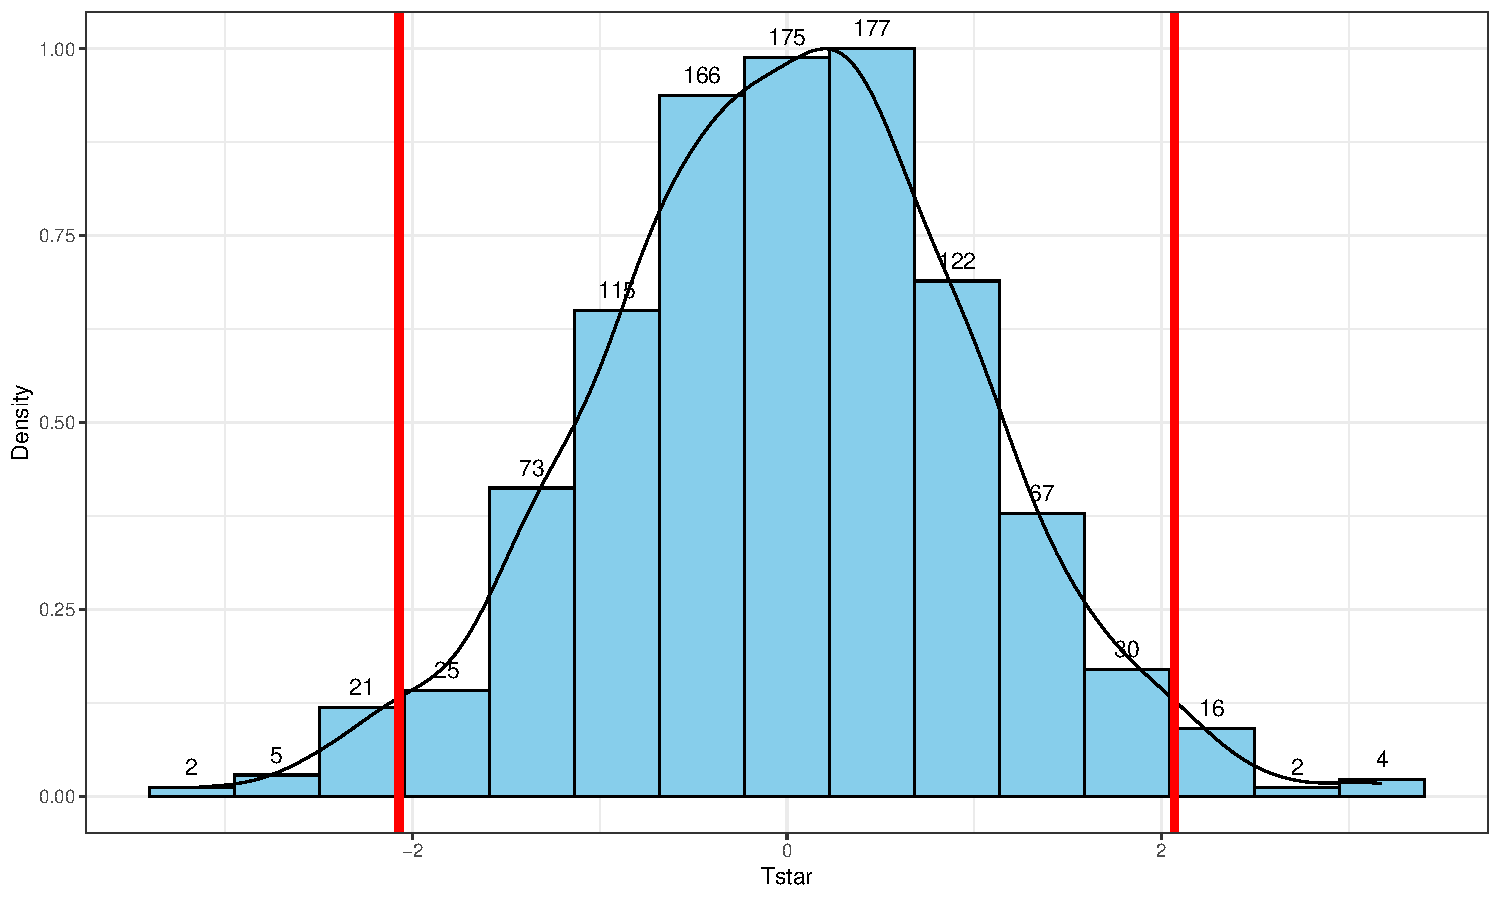
\includegraphics[width=0.75\linewidth]{02-linearmodelsreview_files/figure-latex/Figure2-12-1} 

}

\caption{Permutation distribution of the \(t\)-statistic.}\label{fig:Figure2-12}
\end{figure}

\newpage

\begin{Shaded}
\begin{Highlighting}[]
\FunctionTok{tibble}\NormalTok{(Tstar) }\SpecialCharTok{\%\textgreater{}\%} \FunctionTok{ggplot}\NormalTok{(}\FunctionTok{aes}\NormalTok{(}\AttributeTok{x =}\NormalTok{ Tstar)) }\SpecialCharTok{+} 
  \FunctionTok{geom\_histogram}\NormalTok{(}\FunctionTok{aes}\NormalTok{(}\AttributeTok{y =}\NormalTok{ ..ncount..), }\AttributeTok{bins =} \DecValTok{15}\NormalTok{, }\AttributeTok{col =} \DecValTok{1}\NormalTok{, }\AttributeTok{fill =} \StringTok{"skyblue"}\NormalTok{, }\AttributeTok{center =} \DecValTok{0}\NormalTok{) }\SpecialCharTok{+} 
  \FunctionTok{geom\_density}\NormalTok{(}\FunctionTok{aes}\NormalTok{(}\AttributeTok{y =}\NormalTok{ ..scaled..)) }\SpecialCharTok{+}
  \FunctionTok{theme\_bw}\NormalTok{() }\SpecialCharTok{+}
  \FunctionTok{labs}\NormalTok{(}\AttributeTok{y =} \StringTok{"Density"}\NormalTok{) }\SpecialCharTok{+}
  \FunctionTok{geom\_vline}\NormalTok{(}\AttributeTok{xintercept =} \FunctionTok{c}\NormalTok{(}\SpecialCharTok{{-}}\DecValTok{1}\NormalTok{,}\DecValTok{1}\NormalTok{)}\SpecialCharTok{*}\NormalTok{Tobs, }\AttributeTok{col =} \StringTok{"red"}\NormalTok{, }\AttributeTok{lwd =} \DecValTok{2}\NormalTok{) }\SpecialCharTok{+}
  \FunctionTok{stat\_bin}\NormalTok{(}\FunctionTok{aes}\NormalTok{(}\AttributeTok{y =}\NormalTok{ ..ncount.., }\AttributeTok{label =}\NormalTok{ ..count..), }\AttributeTok{bins =} \DecValTok{15}\NormalTok{, }
           \AttributeTok{geom =} \StringTok{"text"}\NormalTok{, }\AttributeTok{vjust =} \SpecialCharTok{{-}}\FloatTok{0.75}\NormalTok{)}
\end{Highlighting}
\end{Shaded}

\indent The parametric version
\index{parametric}
of these results is based on using what is called
the \textbf{\emph{two-independent sample t-test}}. There are actually two versions of this
test, one that assumes that variances are equal in the groups and one that
does not. There is a rule of thumb that if the \textbf{ratio of the larger standard
deviation over the smaller standard deviation is less than 2, the equal variance
procedure is OK}. It ends up that this assumption
is less important if the sample sizes in the groups are approximately equal
and more important if the groups contain different numbers of observations. In
comparing the two potential test statistics, the procedure that assumes equal
variances has a complicated denominator (see the formula above for \(t\)
involving \(s_p\)) but a simple formula for \textbf{\emph{degrees of freedom}} (\textbf{\emph{df}})
\index{degrees of freedom!t-distribution}
\index{@$t$-distribution}
for the \(t\)-distribution (\(df = n_1+n_2-2\)) that approximates the
distribution of the test statistic, \(t\), under the null hypothesis. The
procedure that assumes unequal variances has a simpler test statistic and a
very complicated degrees of freedom formula. The equal variance procedure is
equivalent to the methods we will consider in Chapters
\ref{chapter3} and \ref{chapter4} so that
will be our focus for the two group problem and is what we get when using the \texttt{lm} model to estimate the differences in the group means. The unequal variance version of the two-sample t-test is available in the \texttt{t.test} function if needed.



\begin{figure}[ht!]

{\centering 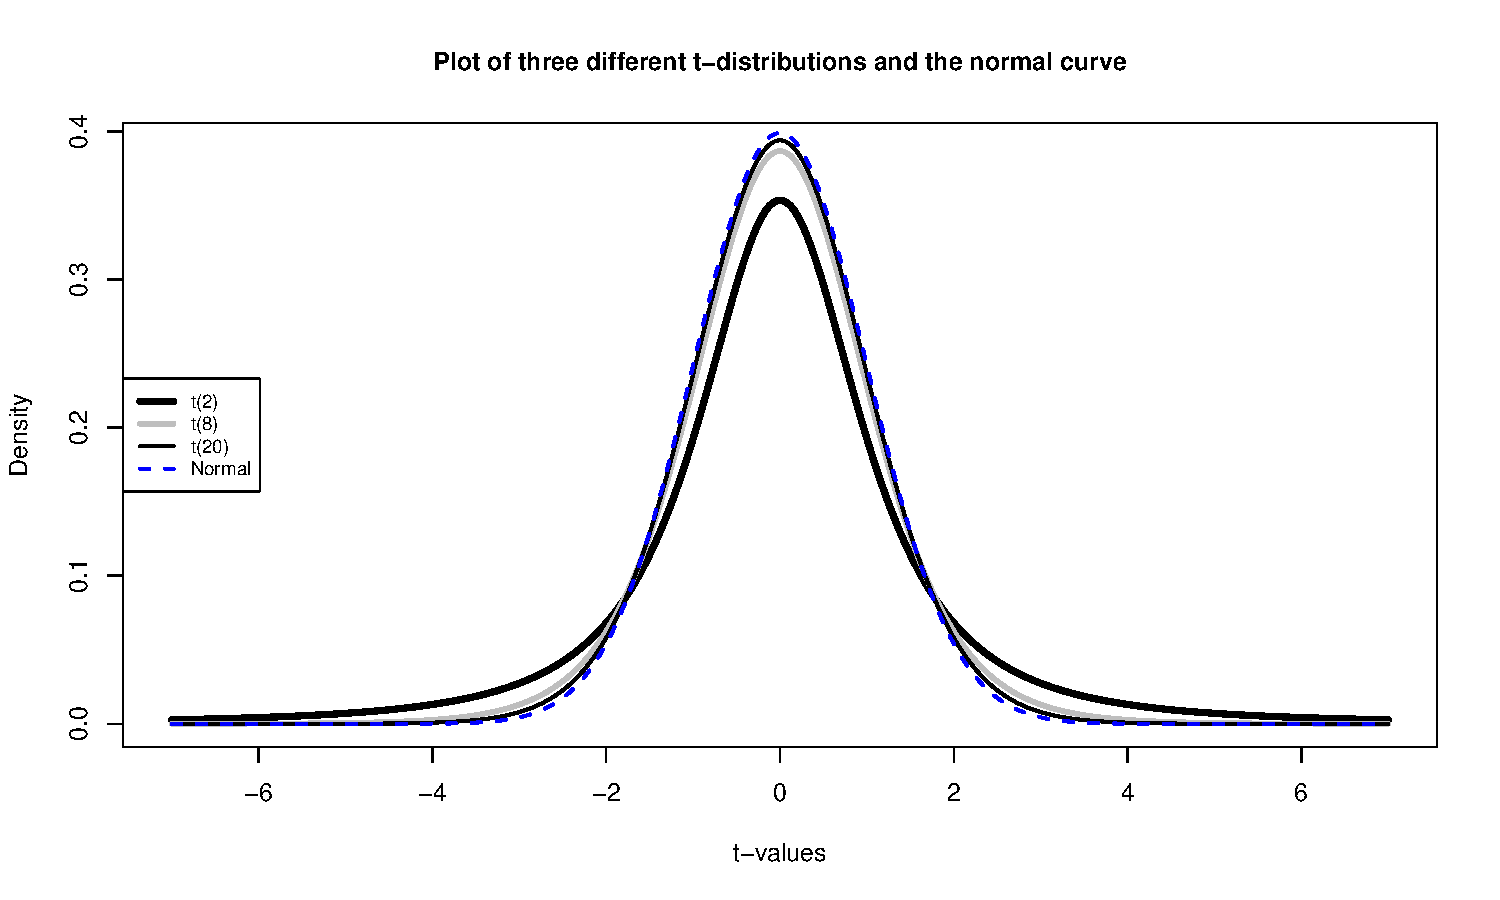
\includegraphics[width=0.75\linewidth]{02-linearmodelsreview_files/figure-latex/Figure2-13-1} 

}

\caption{Plots of \(t\)-distributions with 2, 8, and 20 degrees of freedom and a normal distribution (dashed line). Note how the \(t\)-distributions get closer to the normal distribution as the degrees of freedom increase and at 20 degrees of freedom, the \(t\)-distribution \emph{almost} matches a standard normal curve.}\label{fig:Figure2-13}
\end{figure}

\indent If the assumptions for the equal variance \(t\)-test and the null
hypothesis are true, then the sampling distribution of the test statistic should
follow a \(t\)-distribution
\index{@$t$-distribution}
with \(n_1+n_2-2\) degrees of freedom (so the total sample size, \(n\), minus 2). The \textbf{\emph{t-distribution}} is a bell-shaped curve that is more spread out for smaller
values of degrees of freedom as shown in Figure \ref{fig:Figure2-13}. The
\(t\)-distribution looks more and more like a \textbf{\emph{standard normal distribution}}
\index{standard normal distribution}
(\(N(0,1)\)) as the degrees of freedom increase.

\indent To get the p-value for the parametric \(t\)-test,
\index{p-value!calculation of}
we need to calculate the
test statistic and \(df\), then look up the areas in the tails of the
\(t\)-distribution
\index{@$t$-distribution}
relative to the observed \(t\)-statistic. We'll learn how to use
R to do this below, but for now we will allow the \texttt{summary} of the \texttt{lm} function to take
care of this. In the \texttt{ConditionCommute} row of the summary and the \texttt{Pr(\textgreater{}\textbar{}t\textbar{})} column, we can find the p-value associated with the test statistic. We can either calculate the degrees of freedom for the \(t\)-distribution using \(n_1+n_2-2 = 15+15-2 = 28\) or explore the full suite of the model summary that is repeated below. In the first row below the \texttt{ConditionCommute} row, it reports ``\ldots{} 28 degrees of freedom'' and these are the same \(df\) that are needed to report and look up for any of the \(t\)-statistics in the model summary.

\begin{Shaded}
\begin{Highlighting}[]
\FunctionTok{summary}\NormalTok{(lm1)}
\end{Highlighting}
\end{Shaded}

\begin{verbatim}
## 
## Call:
## lm(formula = Distance ~ Condition, data = dsample)
## 
## Residuals:
##     Min      1Q  Median      3Q     Max 
## -63.800 -21.850   4.133  15.150  72.200 
## 
## Coefficients:
##                  Estimate Std. Error t value Pr(>|t|)
## (Intercept)       135.800      8.863  15.322 3.83e-15
## Conditioncommute  -25.933     12.534  -2.069   0.0479
## 
## Residual standard error: 34.33 on 28 degrees of freedom
## Multiple R-squared:  0.1326, Adjusted R-squared:  0.1016 
## F-statistic: 4.281 on 1 and 28 DF,  p-value: 0.04789
\end{verbatim}

So the parametric \(t\)-test gives a p-value of 0.0479 from a test statistic of
-2.07. The p-value is very similar to the two permutation results found before. The
reason for this similarity is that the permutation distribution looks like a \(t\)-distribution with 28 degrees
of freedom. Figure \ref{fig:Figure2-14} shows how similar the two distributions
happened to be here, where the only difference in shape is near the peak of the distributions with a slight difference of the permutation distribution to shift to the right.



\begin{figure}[ht!]

{\centering 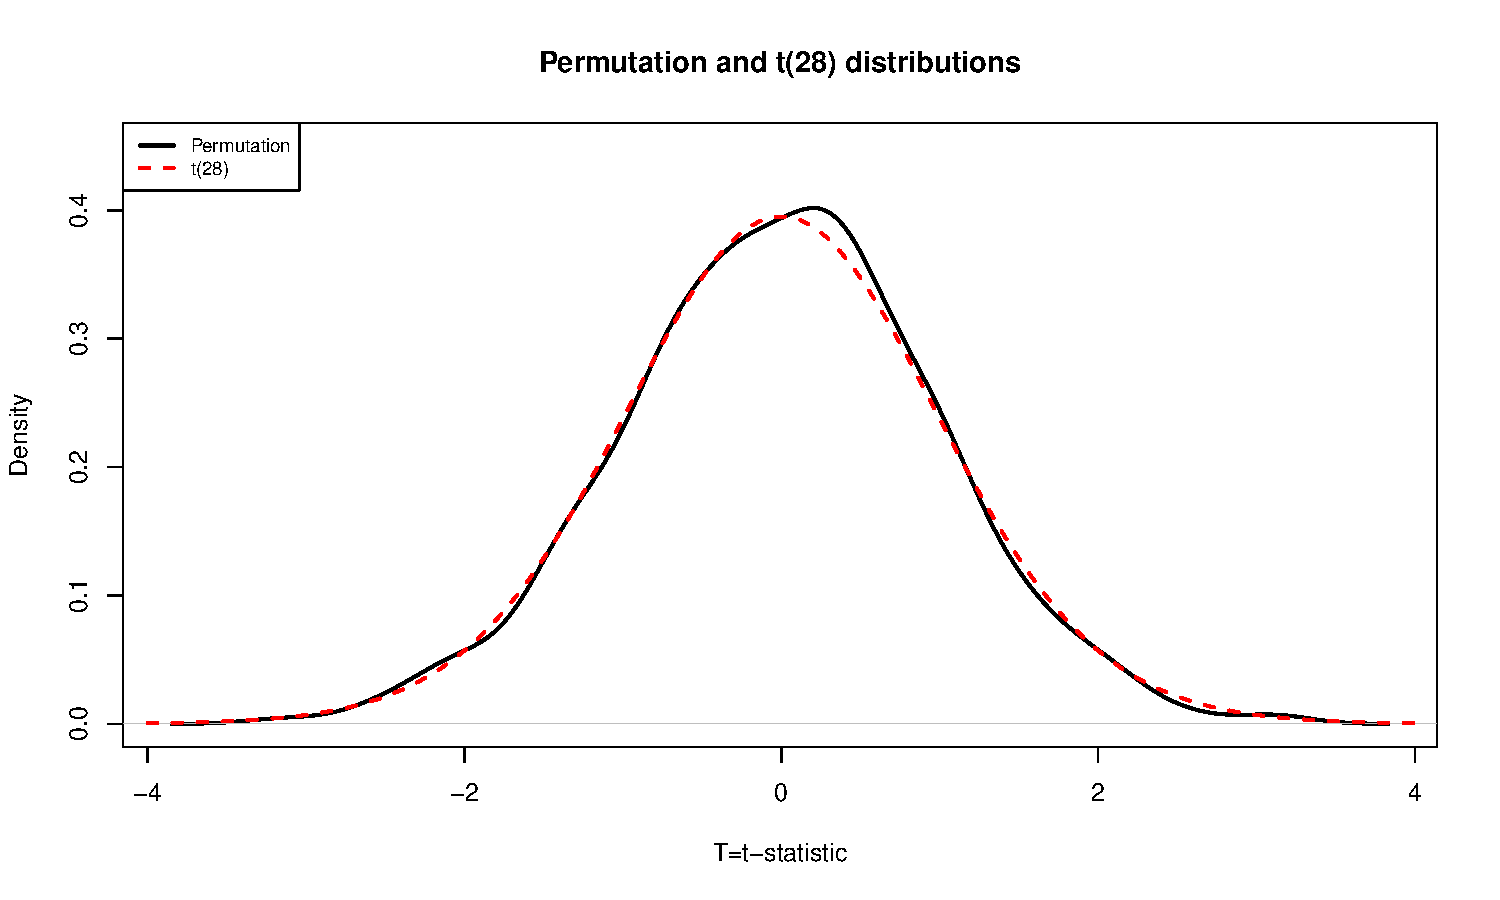
\includegraphics[width=0.75\linewidth]{02-linearmodelsreview_files/figure-latex/Figure2-14-1} 

}

\caption{Plot of permutation and \(t\)-distribution with \(df = 28\). Note the close match in the two distributions, especially in the tails of the distributions where we are obtaining the p-values.}\label{fig:Figure2-14}
\end{figure}

\indent In your previous statistics course, you might have used an applet or
a table to find p-values such as what was provided in the previous R output.
When not directly provided in the output of a function, R can be used to look up
p-values\footnote{On exams, you might be asked to describe the area of interest, sketch a
  picture of the area of interest, and/or note the distribution you would use. Make sure you think about what you are trying to do here as much as learning the mechanics of how to get p-values from R.} from
named distributions such as the \(t\)-distribution. In this case, the distribution
of the test statistic under the null hypothesis is a \(t(28)\) or a \(t\) with 28
degrees of freedom. The \texttt{pt} function is used to get p-values from the
\index{\texttt{pt()}}
\(t\)-distribution in the same manner that \texttt{pdata} could help us to find p-values
from the permutation distribution.
\index{permutation!distribution}
We need to provide the \texttt{df\ =\ ...} and specify
the tail of the distribution of interest using the \texttt{lower.tail} option along
with the cutoff of interest. If we want the area to the left of -2.07:

\begin{Shaded}
\begin{Highlighting}[]
\FunctionTok{pt}\NormalTok{(}\SpecialCharTok{{-}}\FloatTok{2.069}\NormalTok{, }\AttributeTok{df =} \DecValTok{28}\NormalTok{, }\AttributeTok{lower.tail =}\NormalTok{ T)}
\end{Highlighting}
\end{Shaded}

\begin{verbatim}
## [1] 0.02394519
\end{verbatim}

And we can double it to get the p-value that was in the output, because
the \(t\)-distribution is symmetric:
\index{@$t$-distribution}

\begin{Shaded}
\begin{Highlighting}[]
\DecValTok{2}\SpecialCharTok{*}\FunctionTok{pt}\NormalTok{(}\SpecialCharTok{{-}}\FloatTok{2.069}\NormalTok{, }\AttributeTok{df =} \DecValTok{28}\NormalTok{, }\AttributeTok{lower.tail =}\NormalTok{ T)}
\end{Highlighting}
\end{Shaded}

\begin{verbatim}
## [1] 0.04789038
\end{verbatim}

More generally, we could always make the test statistic positive using the
absolute value (\texttt{abs}), find the area to the right of it (\texttt{lower.tail\ =\ F}), and then double that for a
two-sided test p-value:

\begin{Shaded}
\begin{Highlighting}[]
\DecValTok{2}\SpecialCharTok{*}\FunctionTok{pt}\NormalTok{(}\FunctionTok{abs}\NormalTok{(}\SpecialCharTok{{-}}\FloatTok{2.069}\NormalTok{), }\AttributeTok{df =} \DecValTok{28}\NormalTok{, }\AttributeTok{lower.tail =}\NormalTok{ F)}
\end{Highlighting}
\end{Shaded}

\begin{verbatim}
## [1] 0.04789038
\end{verbatim}

\indent Permutation distributions \index{permutation!distribution} do not need to match the named
parametric distribution
\index{parametric!distribution}
to work correctly, although this happened in the previous example.
The parametric approach, the \(t\)-test, requires certain conditions to be true (or at least not be clearly violated)
for the sampling distribution of the
statistic to follow the named distribution and provide accurate p-values. The
conditions for the \(t\)-test are:

\begin{enumerate}
\def\labelenumi{\arabic{enumi}.}
\item
  \textbf{Independent observations}:
  \index{independence assumption!two-independent sample}
  Each observation obtained is unrelated to all other
  observations. To assess this, consider whether anything in the data collection
  might lead to clustered or related observations that are un-related to the
  differences in the groups. For example, was the same person measured more than
  once\footnote{In some studies, the same subject is measured in both conditions and
    this violates the assumptions of this procedure.}?
\item
  \textbf{Equal variances} in the groups (because we used a procedure that assumes
  equal variances! -- there is another procedure that allows you to relax this
  assumption if needed\ldots). To assess this, compare the standard deviations and
  variability in the pirate-plots \index{pirate-plot} and see if they look noticeably different. Be
  particularly critical of this assessment if the sample sizes differ greatly
  between groups.
\item
  \textbf{Normal distributions} of the observations in each group. We'll learn more
  diagnostics later, but the pirate-plots are a good place to start to
  help you look for potential skew or outliers. If you find
  skew and/or outliers, that would suggest a problem with the assumption of
  normality as normal distributions
  \index{normal distribution} \index{outlier} \index{skew}
  are symmetric and extreme observations occur
  very rarely.
\end{enumerate}

For the permutation test, \index{permutation!test} we relax the third condition and replace it with:

\begin{enumerate}
\def\labelenumi{\arabic{enumi}.}
\setcounter{enumi}{2}
\tightlist
\item
  \textbf{\emph{Similar distributions for the groups:}} The permutation approach
  allows valid inferences as long as the two groups have similar shapes and only
  possibly differ in their centers. In other words, the distributions need not
  look normal for the procedure to work well, but they do need to look similar.
  \index{similar distributions}
\end{enumerate}

\indent In the bicycle overtake study, the independent
observation condition is violated because of multiple measurements taken on the same ride. The fact that the same rider was used for all observations is not really a violation of independence here because there was only one subject used. If multiple subjects had been used, then that also could present a violation of the independence assumption. This violation is important to note as the inferences may not be correct due to the violation of this assumption and more sophisticated statistical methods would be needed to complete this analysis correctly. The equal variance condition does not appear to be violated. The standard deviations are 28.4 vs 39.4, so this difference is not ``large''
according to the rule of thumb noted above (ratio of SDs is about 1.4). There is also little evidence in the pirate-plots to suggest a violation of the normality condition for each of the groups (Figure \ref{fig:Figure2-5}). Additionally, the shapes look similar for the two groups so we also could feel comfortable using the permutation approach based on
its version of condition (3) above. Note that when assessing assumptions, it is important to never state that assumptions are met -- we never know the truth and can only look at the information in the sample to look for evidence of problems with particular conditions. Violations of those conditions suggest a need for either more sophisticated statistical tools\footnote{At this level, it is critical to learn the tools and learn where they might provide inaccurate inferences. If you explore more advanced statistical resources, you will encounter methods that can allow you to obtain valid inferences in even more scenarios.} or possibly transformations of the response variable (discussed in Chapter \ref{chapter7}).

\indent The permutation approach is resistant
\index{resistant}
to impacts of violations of the
normality assumption. It is not resistant to impacts of violations of any of
the other assumptions.
\index{assumptions}
In fact, it can be quite sensitive to unequal variances
as it will detect differences in the variances of the groups instead of
differences in the means. Its scope of inference is the same as the parametric
approach. \index{scope of inference} It also provides similarly inaccurate conclusions in the presence
of non-independent observations as for the parametric approach. In this
example, we discover that parametric and permutation approaches provide very
similar inferences, but both are subject to concerns related to violations of the independent observations condition. And we haven't directly addressed the size and direction of the differences, which is addressed in the coming discussion of confidence intervals.

\indent For comparison, we can also explore the original data set of all \(n = 1,636\) observations for the two outfits. The estimated difference in the means is -3.003 cm (\emph{commute} minus \emph{casual}), the standard error is 1.472, the \(t\)-statistic is -2.039 and using a \(t\)-distribution with 1634 \(df\), the p-value is 0.0416. The estimated difference in the means is much smaller but the p-value is similar to the results for the sub-sample we analyzed. The SE is much smaller with the large sample size which corresponds to having higher power to detect smaller differences.

\begin{Shaded}
\begin{Highlighting}[]
\NormalTok{lm\_all }\OtherTok{\textless{}{-}} \FunctionTok{lm}\NormalTok{(Distance }\SpecialCharTok{\textasciitilde{}}\NormalTok{ Condition, }\AttributeTok{data =}\NormalTok{ ddsub)}
\FunctionTok{summary}\NormalTok{(lm\_all)}
\end{Highlighting}
\end{Shaded}

\begin{verbatim}
## 
## Call:
## lm(formula = Distance ~ Condition, data = ddsub)
## 
## Residuals:
##      Min       1Q   Median       3Q      Max 
## -106.608  -17.608    0.389   16.392  127.389 
## 
## Coefficients:
##                  Estimate Std. Error t value Pr(>|t|)
## (Intercept)       117.611      1.066 110.357   <2e-16
## Conditioncommute   -3.003      1.472  -2.039   0.0416
## 
## Residual standard error: 29.75 on 1634 degrees of freedom
## Multiple R-squared:  0.002539,   Adjusted R-squared:  0.001929 
## F-statistic:  4.16 on 1 and 1634 DF,  p-value: 0.04156
\end{verbatim}

The permutations take a little more computing power with almost two thousand observations to shuffle, but this is manageable on a modern laptop as it only has to be completed once to fill in the distribution of the test statistic under 1,000 shuffles. And the p-value obtained is a close match to the parametric result at 0.045 for the permutation version and 0.042 for the parametric approach. So we would get similar inferences for strength of evidence against the null with either the smaller data set or the full data set but the estimated size of the differences is quite a bit different. It is important to note that other random samples from the larger data set would give different p-values and this one happened to match the larger set more closely than one might expect in general.

\begin{Shaded}
\begin{Highlighting}[]
\NormalTok{Tobs }\OtherTok{\textless{}{-}} \FunctionTok{summary}\NormalTok{(lm\_all)}\SpecialCharTok{$}\NormalTok{coef[}\DecValTok{2}\NormalTok{,}\DecValTok{3}\NormalTok{]}
\NormalTok{Tobs}
\end{Highlighting}
\end{Shaded}

\begin{verbatim}
## [1] -2.039491
\end{verbatim}

\begin{Shaded}
\begin{Highlighting}[]
\NormalTok{B }\OtherTok{\textless{}{-}} \DecValTok{1000}
\FunctionTok{set.seed}\NormalTok{(}\DecValTok{406}\NormalTok{)}
\NormalTok{Tstar }\OtherTok{\textless{}{-}} \FunctionTok{matrix}\NormalTok{(}\ConstantTok{NA}\NormalTok{, }\AttributeTok{nrow =}\NormalTok{ B)}
\ControlFlowTok{for}\NormalTok{ (b }\ControlFlowTok{in}\NormalTok{ (}\DecValTok{1}\SpecialCharTok{:}\NormalTok{B))\{}
\NormalTok{  lmP }\OtherTok{\textless{}{-}} \FunctionTok{lm}\NormalTok{(Distance }\SpecialCharTok{\textasciitilde{}} \FunctionTok{shuffle}\NormalTok{(Condition), }\AttributeTok{data =}\NormalTok{ ddsub)}
\NormalTok{  Tstar[b] }\OtherTok{\textless{}{-}} \FunctionTok{summary}\NormalTok{(lmP)}\SpecialCharTok{$}\NormalTok{coef[}\DecValTok{2}\NormalTok{,}\DecValTok{3}\NormalTok{]}
\NormalTok{\}}
\FunctionTok{pdata}\NormalTok{(}\FunctionTok{abs}\NormalTok{(Tstar), }\FunctionTok{abs}\NormalTok{(Tobs), }\AttributeTok{lower.tail =}\NormalTok{ F)}
\end{Highlighting}
\end{Shaded}

\begin{verbatim}
## [1] 0.045
\end{verbatim}



\begin{figure}[ht!]

{\centering 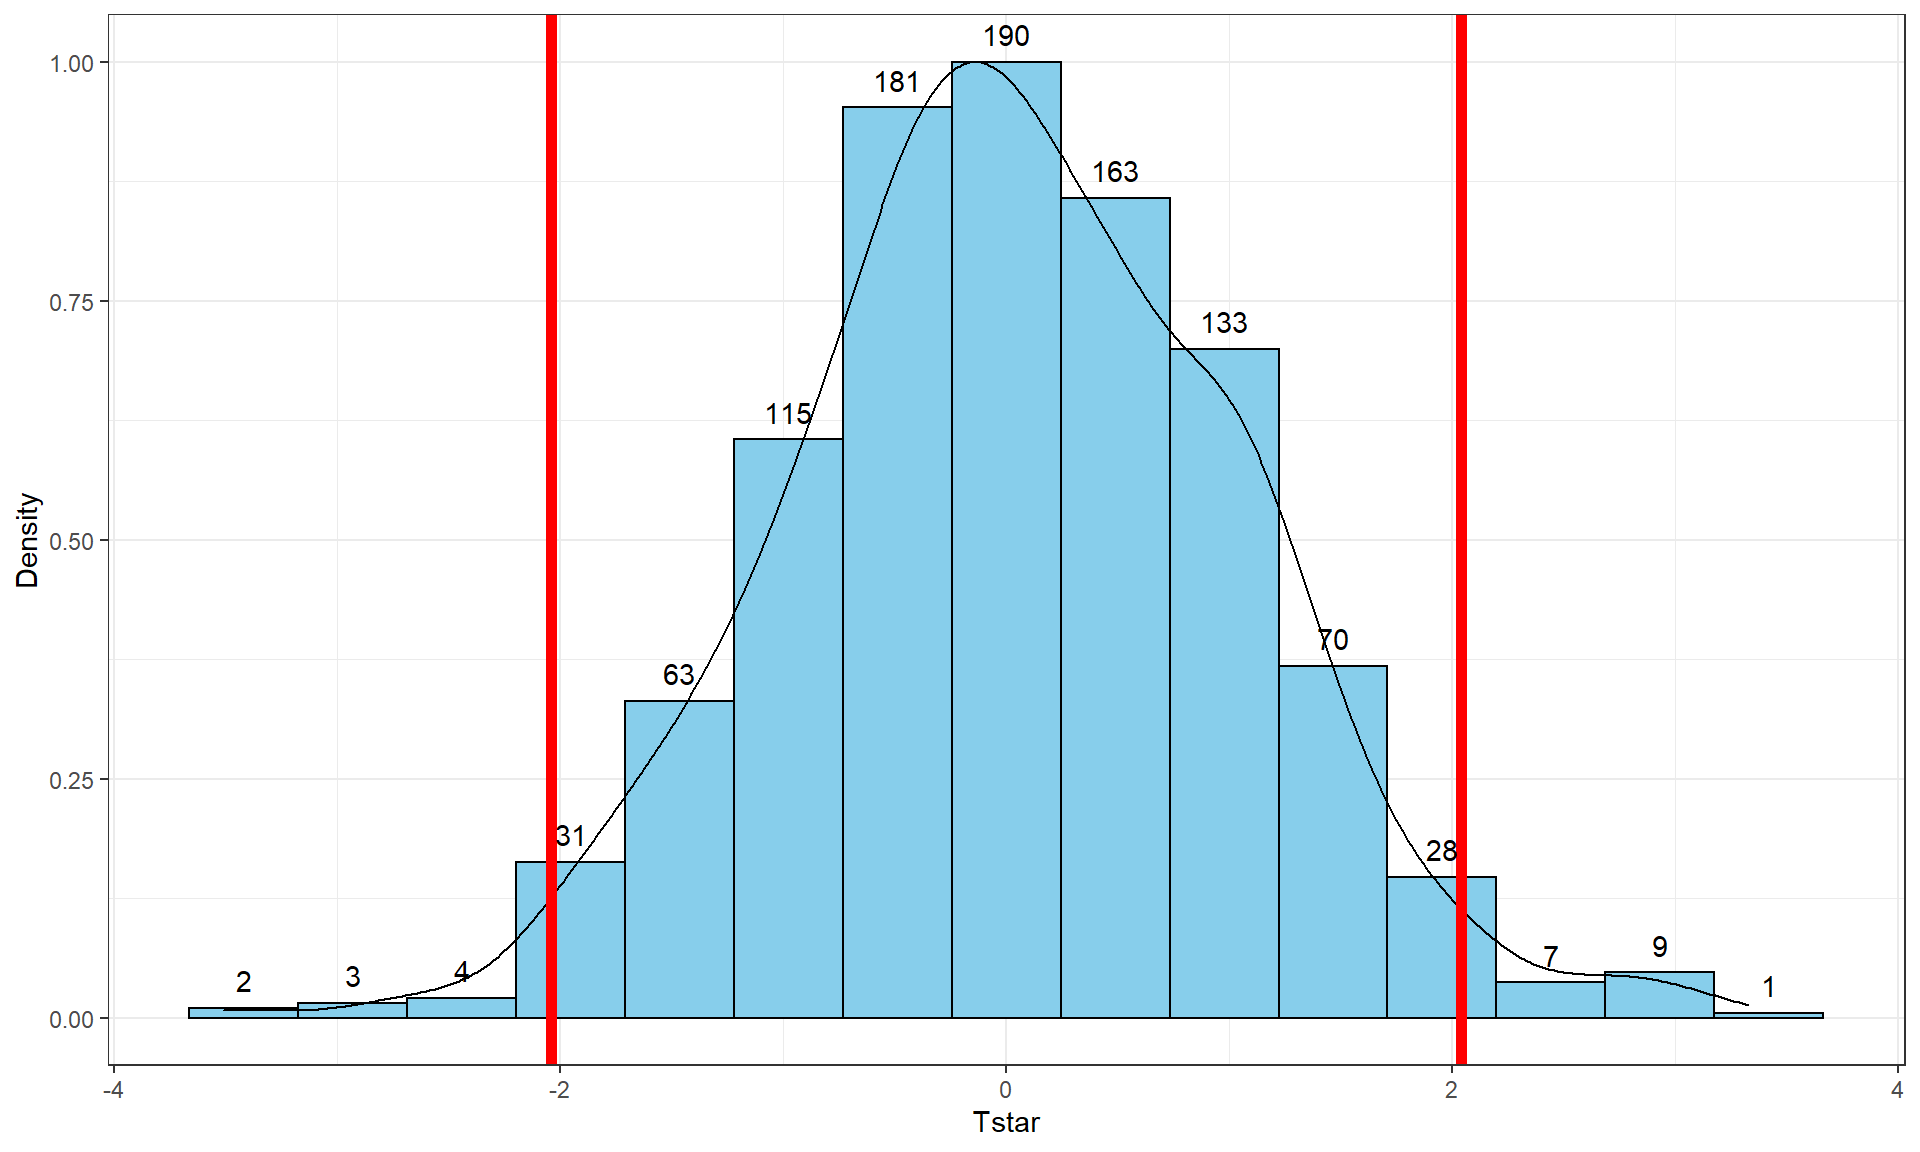
\includegraphics[width=0.75\linewidth]{02-linearmodelsreview_files/figure-latex/Figure2-15-1} 

}

\caption{Permutation distribution of the \(t\)-statistic for \(n = 1,636\) overtake data set.}\label{fig:Figure2-15}
\end{figure}

\newpage

\hypertarget{section2-7}{%
\section{Second example of permutation tests}\label{section2-7}}

In every chapter, the first example, used to motivate and explain
the methods, is followed with a ``worked'' example where we focus just on the
results. In a
previous semester, some of the Intermediate Statistics (STAT 217) students at Montana State University (\textbf{\emph{n}} = 79) provided
information on their \emph{Sex}\footnote{Only male and female were provided as options on the survey. These data were collected as part of a project to study learning of material using online versus paper versions of this book but we focus just on the gender differences in GPA here.}, \emph{Age}, and current cumulative \emph{GPA}. We might be
interested in whether Males and Females had different average GPAs. First,
we can take a look at the difference in the responses by groups based on the
output and as displayed in Figure \ref{fig:Figure2-16}.

\begin{Shaded}
\begin{Highlighting}[]
\NormalTok{s217 }\OtherTok{\textless{}{-}} \FunctionTok{read\_csv}\NormalTok{(}\StringTok{"http://www.math.montana.edu/courses/s217/documents/s217.csv"}\NormalTok{)}
\FunctionTok{library}\NormalTok{(mosaic)}
\FunctionTok{library}\NormalTok{(yarrr)}
\end{Highlighting}
\end{Shaded}

\begin{Shaded}
\begin{Highlighting}[]
\FunctionTok{mean}\NormalTok{(GPA }\SpecialCharTok{\textasciitilde{}}\NormalTok{ Sex, }\AttributeTok{data =}\NormalTok{ s217)}
\end{Highlighting}
\end{Shaded}

\begin{verbatim}
##        F        M 
## 3.338378 3.088571
\end{verbatim}

\begin{Shaded}
\begin{Highlighting}[]
\FunctionTok{favstats}\NormalTok{(GPA }\SpecialCharTok{\textasciitilde{}}\NormalTok{ Sex, }\AttributeTok{data =}\NormalTok{ s217)}
\end{Highlighting}
\end{Shaded}

\begin{verbatim}
##   Sex  min  Q1 median   Q3 max     mean        sd  n missing
## 1   F 2.50 3.1  3.400 3.70   4 3.338378 0.4074549 37       0
## 2   M 1.96 2.8  3.175 3.46   4 3.088571 0.4151789 42       0
\end{verbatim}



\begin{figure}[ht!]

{\centering 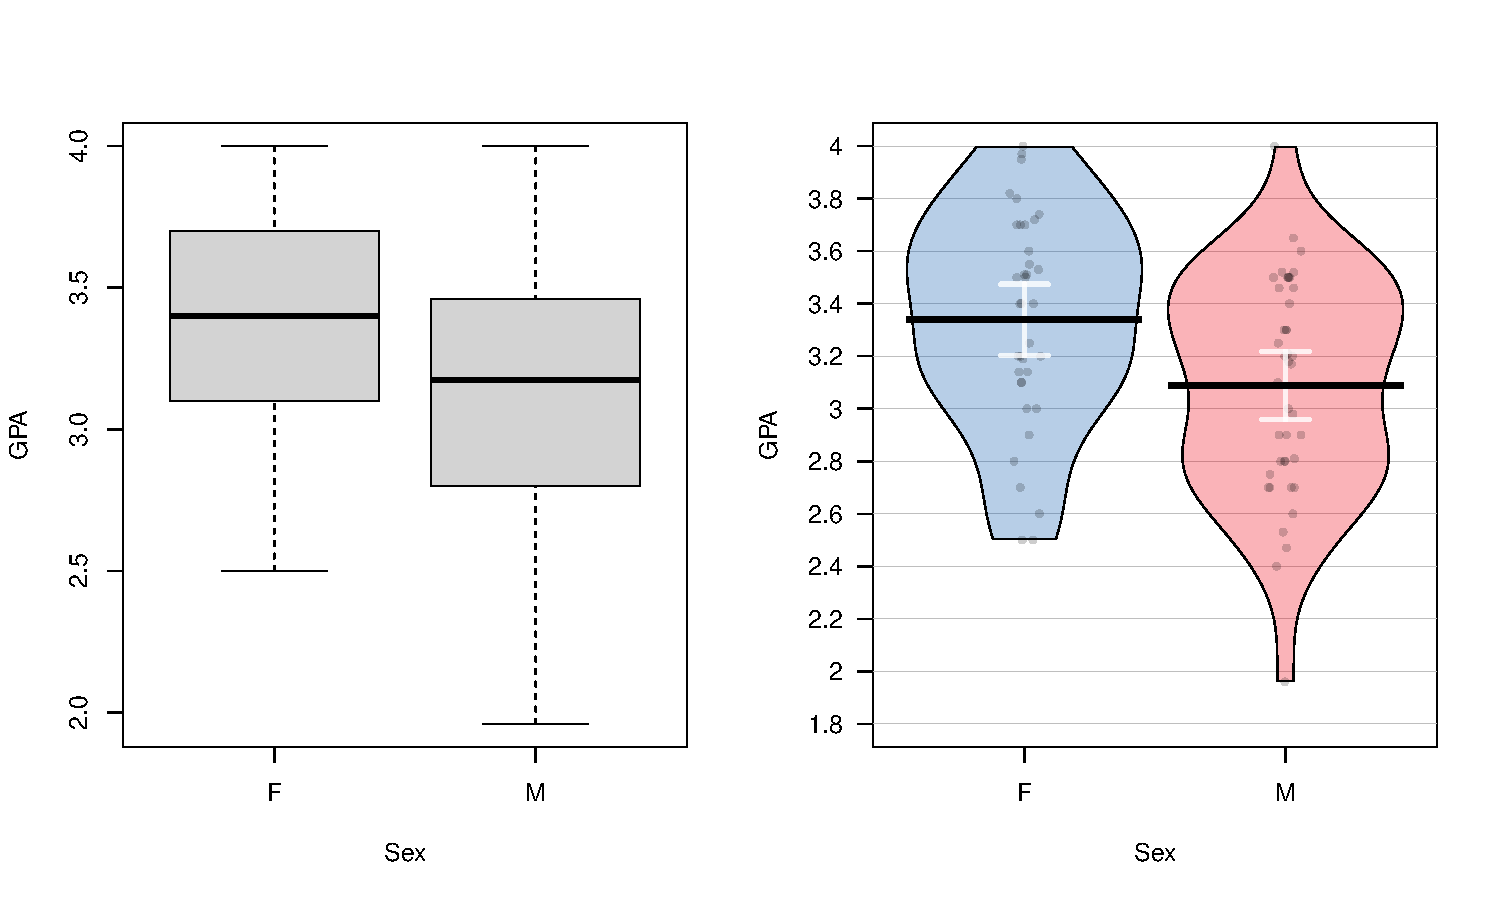
\includegraphics[width=0.75\linewidth]{02-linearmodelsreview_files/figure-latex/Figure2-16-1} 

}

\caption{Side-by-side boxplot and pirate-plot of GPAs of Intermediate Statistics students by gender.}\label{fig:Figure2-16}
\end{figure}

\begin{Shaded}
\begin{Highlighting}[]
\FunctionTok{boxplot}\NormalTok{(GPA }\SpecialCharTok{\textasciitilde{}}\NormalTok{ Sex, }\AttributeTok{data =}\NormalTok{ s217)}
\FunctionTok{pirateplot}\NormalTok{(GPA }\SpecialCharTok{\textasciitilde{}}\NormalTok{ Sex, }\AttributeTok{data =}\NormalTok{ s217, }\AttributeTok{inf.method =} \StringTok{"ci"}\NormalTok{, }\AttributeTok{inf.disp =} \StringTok{"line"}\NormalTok{)}
\end{Highlighting}
\end{Shaded}

In these data, the distributions of the GPAs look to be left skewed. The
Female GPAs look to be slightly higher than for Males (0.25 GPA difference in the
means) but is that a ``real'' difference? We need our inference tools to more fully
assess these differences.

\indent First, we can try the parametric approach:

\begin{Shaded}
\begin{Highlighting}[]
\NormalTok{lm\_GPA }\OtherTok{\textless{}{-}} \FunctionTok{lm}\NormalTok{(GPA }\SpecialCharTok{\textasciitilde{}}\NormalTok{ Sex, }\AttributeTok{data =}\NormalTok{ s217)}
\FunctionTok{summary}\NormalTok{(lm\_GPA)}
\end{Highlighting}
\end{Shaded}

\begin{verbatim}
## 
## Call:
## lm(formula = GPA ~ Sex, data = s217)
## 
## Residuals:
##      Min       1Q   Median       3Q      Max 
## -1.12857 -0.28857  0.06162  0.36162  0.91143 
## 
## Coefficients:
##             Estimate Std. Error t value Pr(>|t|)
## (Intercept)  3.33838    0.06766  49.337  < 2e-16
## SexM        -0.24981    0.09280  -2.692  0.00871
## 
## Residual standard error: 0.4116 on 77 degrees of freedom
## Multiple R-squared:  0.08601,    Adjusted R-squared:  0.07414 
## F-statistic: 7.246 on 1 and 77 DF,  p-value: 0.008713
\end{verbatim}

So the test statistic was observed to be \(t = 2.69\) and it hopefully
follows a \(t(77)\) distribution under the null hypothesis. This provides a
p-value of 0.008713 that we can trust if the conditions to use this
procedure are at least not clearly violated.
Compare these results to the permutation approach, which relaxes that normality
assumption, with the results that follow. In the permutation test, \(T = -2.692\) and
the p-value is 0.011 which is a little larger than the result provided
by the parametric approach. The general agreement of the two approaches, again, provides
some re-assurance about the use of either approach when there are not dramatic violations of validity conditions. \index{permutation!test}

\begin{Shaded}
\begin{Highlighting}[]
\NormalTok{B }\OtherTok{\textless{}{-}} \DecValTok{1000}
\NormalTok{Tobs }\OtherTok{\textless{}{-}} \FunctionTok{summary}\NormalTok{(lm\_GPA)}\SpecialCharTok{$}\NormalTok{coef[}\DecValTok{2}\NormalTok{,}\DecValTok{3}\NormalTok{]}
\NormalTok{Tstar }\OtherTok{\textless{}{-}} \FunctionTok{matrix}\NormalTok{(}\ConstantTok{NA}\NormalTok{, }\AttributeTok{nrow =}\NormalTok{ B)}
\ControlFlowTok{for}\NormalTok{ (b }\ControlFlowTok{in}\NormalTok{ (}\DecValTok{1}\SpecialCharTok{:}\NormalTok{B))\{}
\NormalTok{  lmP }\OtherTok{\textless{}{-}} \FunctionTok{lm}\NormalTok{(GPA }\SpecialCharTok{\textasciitilde{}} \FunctionTok{shuffle}\NormalTok{(Sex), }\AttributeTok{data =}\NormalTok{ s217)}
\NormalTok{  Tstar[b] }\OtherTok{\textless{}{-}} \FunctionTok{summary}\NormalTok{(lmP)}\SpecialCharTok{$}\NormalTok{coef[}\DecValTok{2}\NormalTok{,}\DecValTok{3}\NormalTok{]}
\NormalTok{\}}
\FunctionTok{pdata}\NormalTok{(}\FunctionTok{abs}\NormalTok{(Tstar), }\FunctionTok{abs}\NormalTok{(Tobs), }\AttributeTok{lower.tail =}\NormalTok{ F)[[}\DecValTok{1}\NormalTok{]]}
\end{Highlighting}
\end{Shaded}

\begin{verbatim}
## [1] 0.011
\end{verbatim}



\begin{figure}[ht!]

{\centering 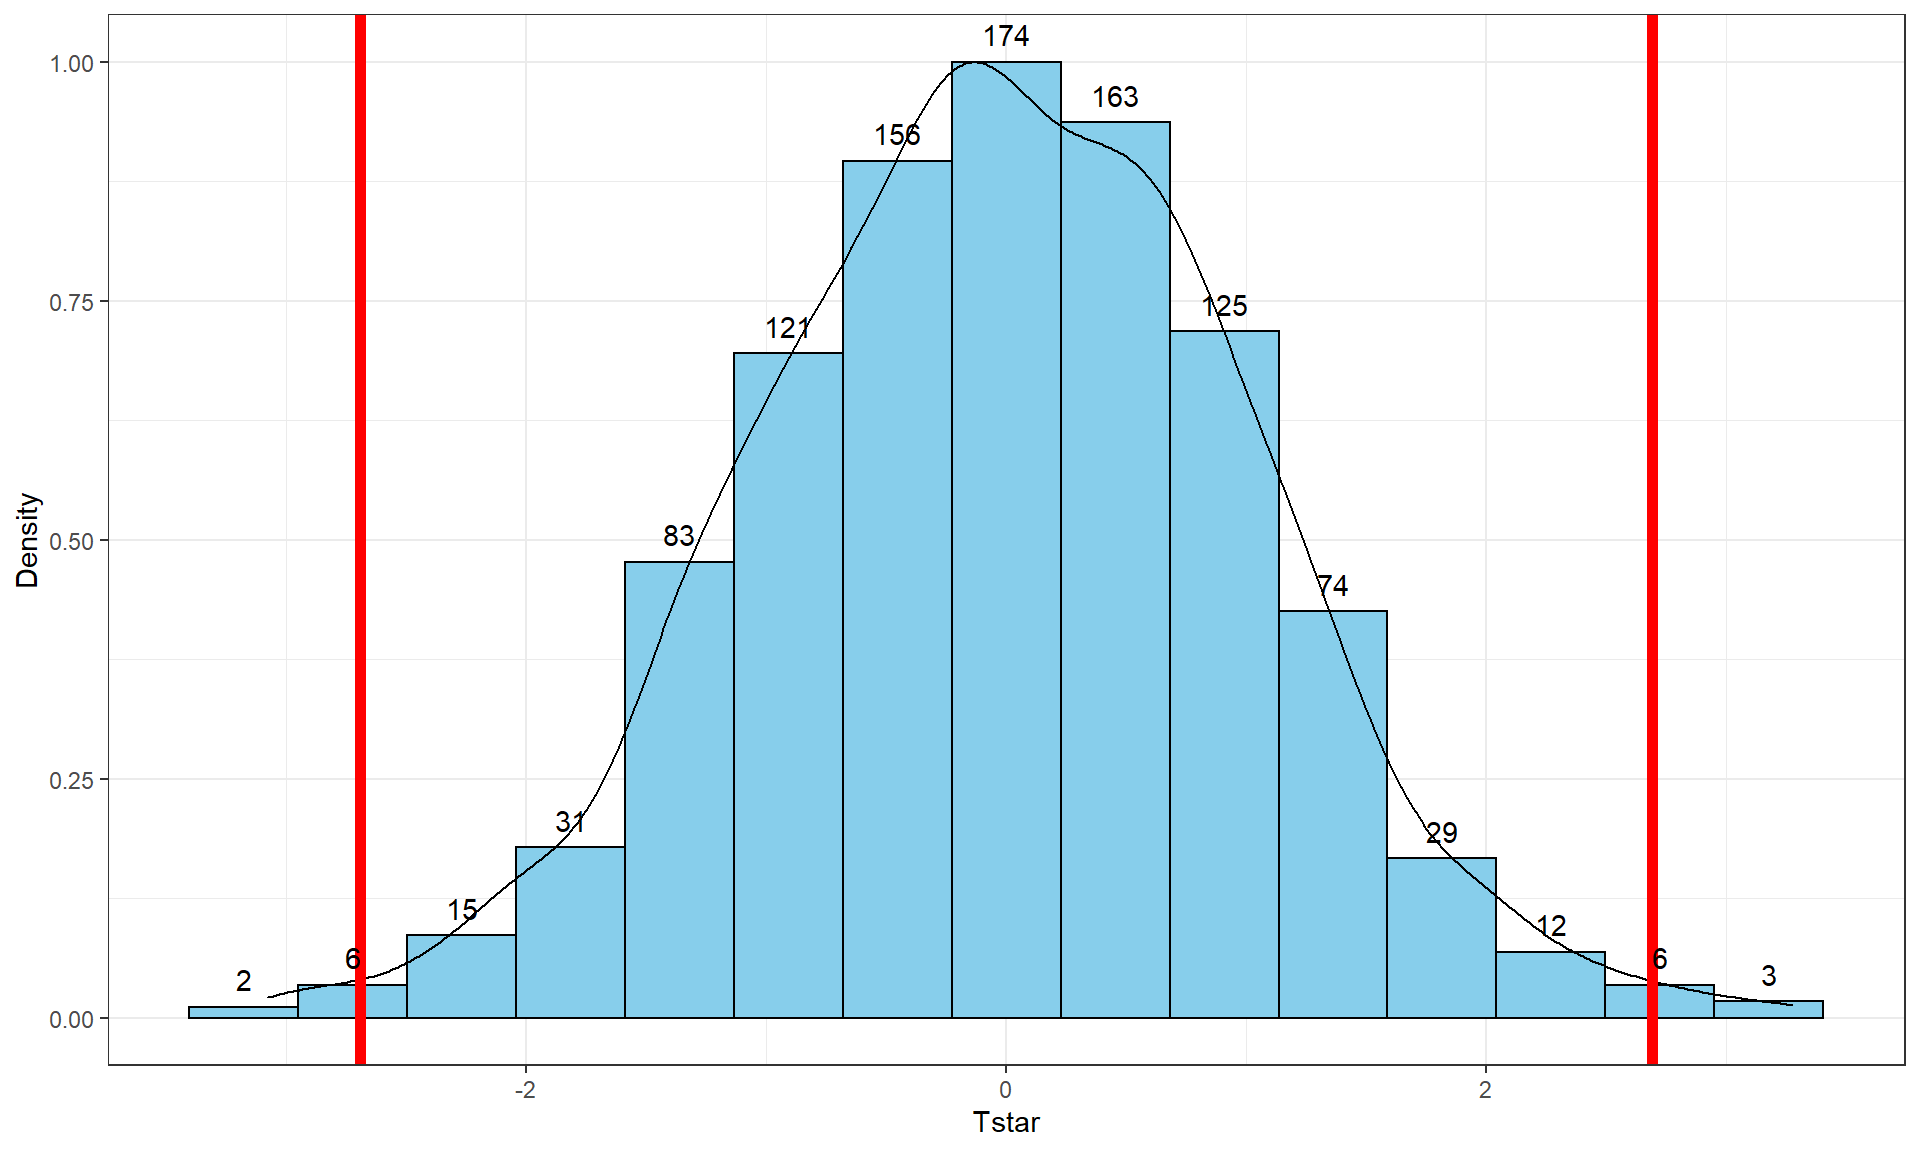
\includegraphics[width=0.75\linewidth]{02-linearmodelsreview_files/figure-latex/Figure2-17-1} 

}

\caption{Histogram and density curve of permutation distribution of test statistic for Intermediate Statistics student GPAs.}\label{fig:Figure2-17}
\end{figure}

\begin{Shaded}
\begin{Highlighting}[]
\FunctionTok{tibble}\NormalTok{(Tstar) }\SpecialCharTok{\%\textgreater{}\%} \FunctionTok{ggplot}\NormalTok{(}\FunctionTok{aes}\NormalTok{(}\AttributeTok{x =}\NormalTok{ Tstar)) }\SpecialCharTok{+} 
  \FunctionTok{geom\_histogram}\NormalTok{(}\FunctionTok{aes}\NormalTok{(}\AttributeTok{y =}\NormalTok{ ..ncount..), }\AttributeTok{bins =} \DecValTok{15}\NormalTok{, }\AttributeTok{col =} \DecValTok{1}\NormalTok{, }\AttributeTok{fill =} \StringTok{"skyblue"}\NormalTok{, }\AttributeTok{center =} \DecValTok{0}\NormalTok{) }\SpecialCharTok{+} 
  \FunctionTok{geom\_density}\NormalTok{(}\FunctionTok{aes}\NormalTok{(}\AttributeTok{y =}\NormalTok{ ..scaled..)) }\SpecialCharTok{+}
  \FunctionTok{theme\_bw}\NormalTok{() }\SpecialCharTok{+}
  \FunctionTok{labs}\NormalTok{(}\AttributeTok{y =} \StringTok{"Density"}\NormalTok{) }\SpecialCharTok{+}
  \FunctionTok{geom\_vline}\NormalTok{(}\AttributeTok{xintercept =} \FunctionTok{c}\NormalTok{(}\SpecialCharTok{{-}}\DecValTok{1}\NormalTok{,}\DecValTok{1}\NormalTok{)}\SpecialCharTok{*}\NormalTok{Tobs, }\AttributeTok{col =} \StringTok{"red"}\NormalTok{, }\AttributeTok{lwd =} \DecValTok{2}\NormalTok{) }\SpecialCharTok{+}
  \FunctionTok{stat\_bin}\NormalTok{(}\FunctionTok{aes}\NormalTok{(}\AttributeTok{y =}\NormalTok{ ..ncount.., }\AttributeTok{label =}\NormalTok{ ..count..), }\AttributeTok{bins =} \DecValTok{15}\NormalTok{, }
           \AttributeTok{geom =} \StringTok{"text"}\NormalTok{, }\AttributeTok{vjust =} \SpecialCharTok{{-}}\FloatTok{0.75}\NormalTok{)}
\end{Highlighting}
\end{Shaded}

Here is a full write-up of the results using all 6+ hypothesis testing
\index{hypothesis testing}
steps,
using the permutation \index{permutation} results for the grade data:

\begin{enumerate}
\def\labelenumi{\arabic{enumi}.}
\setcounter{enumi}{-1}
\item
  The research question involves exploring differences in GPAs between males and females. With data collected from both groups, we should be able to assess this RQ. The pirate-plot with GPAs by gender is a useful visualization. We could use either differences in the sample means or the \(t\)-statistic for the test statistic here.
\item
  Write the null and alternative hypotheses:

  \begin{itemize}
  \item
    \(H_0: \mu_\text{male} = \mu_\text{female}\)

    \begin{itemize}
    \tightlist
    \item
      where \(\mu_\text{male}\) is the true mean GPA for males and
      \(\mu_\text{female}\) is true mean GPA for females.
    \end{itemize}
  \item
    \(H_A: \mu_\text{male} \ne \mu_\text{female}\)
  \end{itemize}
\item
  Plot the data and assess the ``Validity Conditions'' for the procedure being used:

  \begin{itemize}
  \item
    \textbf{Independent observations condition}: It does not appear that this assumption
    is violated because there is no reason to assume any clustering or grouping of
    responses that might create dependence in the observations. The only
    possible consideration is that the observations were taken from different
    sections and there could be some differences among the sections. However,
    for overall GPA there is not too much likelihood that the overall GPAs
    would vary greatly so this not likely to be a big issue. However, it is possible that certain sections (times of day) attract
    students with different GPA levels.
  \item
    \textbf{Equal variance condition}: There is a small difference in the range
    of the observations in the two groups but the standard deviations are very
    similar (close to 0.41) so there is little evidence that this condition is violated.
  \item
    \textbf{Similar distribution condition}: Based on the side-by-side boxplots and
    pirate-plots, it appears that both groups have slightly left-skewed
    distributions, which could be problematic for the parametric approach. The two distributions are not exactly alike but
    they are similar enough that the permutation approach condition is not clearly violated.
  \end{itemize}
\item
  Find the value of the appropriate test statistic and p-value for your hypotheses:

  \begin{itemize}
  \item
    \(T = -2.69\) from the previous R output.
  \item
    p-value \(=\) 0.011 from the permutation distribution results.
  \item
    This means that there is about a 1.1\% chance we would observe
    a difference in mean GPA (female-male or male-female) of 0.25 points or more
    if there in fact is no difference in true mean GPA between females and males
    in Intermediate Statistics in a particular semester.
  \end{itemize}
\item
  Write a conclusion specific to the problem based on the p-value:

  \begin{itemize}
  \tightlist
  \item
    There is strong evidence against the null hypothesis of no difference
    in the true mean GPA between males and females for the Intermediate Statistics students
    in this semester and so we conclude that there is a difference
    in the mean GPAs between males and females in these students.
  \end{itemize}
\end{enumerate}

\begin{enumerate}
\def\labelenumi{\arabic{enumi}.}
\setcounter{enumi}{4}
\item
  Report and discuss an estimate of the size of the differences, with confidence interval(s) if appropriate. \index{size interpretation}

  \begin{itemize}
  \tightlist
  \item
    Females were estimated to have a higher mean GPA by 0.25 points. The next
    section discusses confidence intervals that we could add to this result to
    quantify the uncertainty in this estimate since an estimate without any idea of its precision is only a partial result. This difference of 0.25 on a GPA scale does not seem like a very large difference in the means even though we were able to detect a difference in the groups.
  \end{itemize}
\end{enumerate}

\begin{enumerate}
\def\labelenumi{\arabic{enumi}.}
\setcounter{enumi}{5}
\item
  Scope of inference: \index{scope of inference}

  \begin{itemize}
  \tightlist
  \item
    Because this was not a randomized experiment \index{random assignment} in our explanatory variable, we can't say that the
    difference in gender causes the difference in mean GPA. Because it was
    not a random sample from a larger population (they were asked to participate but not required to and not all the students did participate), our inferences only pertain
    the Intermediate Statistics students that responded to the survey in that semester. \index{random sampling}
  \end{itemize}
\end{enumerate}

\newpage

\hypertarget{section2-8}{%
\section{Reproducibility Crisis: Moving beyond p \textless{} 0.05, publication bias, and multiple testing issues}\label{section2-8}}

In the previous examples, some variation in p-values was observed as different methods (parametric, nonparametric) were applied to the same data set and in the permutation approach, the p-values can vary as well from one set of permutations to another. P-values also vary based on randomness in the data that were collected -- take a different (random) sample and you will get different data and a different p-value. We want the best estimate of a p-value we can obtain, so should use the best sampling method and inference technique that we can. But it is just an estimate of the evidence against the null hypothesis. These sources of variability make fixed \(\alpha\) NHST especially worry-some as sampling variability could take a p-value from just below to just above \(\alpha\) and this would lead to completely different inferences if the only focus is on rejecting the null hypothesis at a fixed significance level. But viewing p-values on a gradient from extremely strong (close to 0) to no (1) evidence against the null hypothesis, p-values of, say, 0.046 and 0.054 provide basically the same evidence against the null hypothesis. The fixed \(\alpha\) decision-making is tied into the use of the terminology of ``significant results'' or, slightly better, ``statistically significant results'' \index{statistically significant} that are intended to convey that there was sufficient evidence to reject the null hypothesis at some pre-decided \(\alpha\) level. You will notice that this is the only time that the ``s-word'' (significant) is considered here.

\index{p-value!criticism}

\indent The focus on p-values has been criticized for a suite of reasons (\protect\hyperlink{ref-Wasserstein2016}{Wasserstein and Lazar 2016}). There are situations when p-values do not address the question of interest or the fact that a small p-value was obtained is so un-surprising that one wonders why it was even reported. For example, in Smith (\protect\hyperlink{ref-Smith2014}{Smith 2014}) the researcher considered bee sting pain ratings across 27 different body locations\footnote{The data are provided and briefly discussed in the Practice Problems for Chapter \ref{chapter3}.}. I don't think anyone would be surprised to learn that there was strong evidence against the null hypothesis of no difference in the true mean pain ratings across different body locations. What is really of interest are the differences in the means -- especially which locations are most painful and how much more painful those locations were than others, on average.

\indent As a field, Statistics is trying to encourage a move away from the focus on p-values and the use of the term ``significant'', even when modified by ``statistically''. There are a variety of reasons for this change. Science (especially in research going into academic journals and in some introductory statistics books) has taken to using p-value \textless{} 0.05 and rejected null hypotheses as the only way to ``certify'' that a result is interesting. It has (and unfortunately still is) hard to publish a paper with a primary result with a p-value that is higher than 0.05, even if the p-value is close to that ``magical'' threshold. One thing that is lost when using that strict cut-off for decisions is that any p-value that is not exactly 1 suggests that there is at least some evidence against the null hypothesis in the data and that evidence is then on a continuum from none to very strong. And that p-values are both a function of the size of the difference and the sample size. It is easy to get small p-values for small size differences with large data sets. A small p-value can be associated with an unimportant (not practically meaningful) size difference. And large p-values, especially in smaller sample situations, could be associated with very meaningful differences in size even though evidence is not strong against the null hypothesis. It is critical to always try to estimate and discuss the size of the differences, whether a large or small p-value is encountered.

\indent There are some other related issues to consider in working with p-values that help to illustrate some of the issues with how p-values and ``statistical significance'' are used in practice. In many studies, researchers have a suite of outcome variables that they measure on their subjects. For example, in an agricultural experiment they might measure the yield of the crops, the protein concentration, the digestibility, and other characteristics of the crops. In various ``omics'' fields such as genomics, proteomics, and metabolomics, responses for each subject on hundreds, thousands, or even millions of variables are considered and a p-value may be generated for each of those variables. In education, researchers might be interested in impacts on grades (as in the previous discussion) but we could also be interested in reading comprehension, student interest in the subject, and the amount of time spent studying, each as response variables in their own right. In each of these situations it means that we are considering not just one null hypothesis and assessing evidence against it, but are doing it many times, from just a few to millions of repetitions. There are two aspects of this process and implications for research to explore further: the impacts on scientific research of focusing solely on ``statistically significant'' results and the impacts of considering more than one hypothesis test in the same study.

\indent There is the systematic bias in scientific research that has emerged from scientists having a difficult time publishing research if p-values for their data are not smaller than 0.05. This has two implications. Many researchers have assumed that results with ``large'' p-values are not interesting -- so they either exclude these results from papers (they put them in \emph{their} file drawer instead of into their papers -- the so-called ``file-drawer'' bias) \index{file-drawer bias} or reviewers reject papers because they did not have small p-values to support their discussions (only results with small p-values are judged as being of interest for publication -- the so-called ``publication bias''). \index{publication bias} Some also include bias from researchers only choosing to move forward with attempting to publish results if they are in the same direction that the researchers expect/theorized as part of this problem -- ignoring results that contradict their theories is an example of ``confirmation bias'' \index{confirmation bias} but also would hinder the evolution of scientific theories to ignore contradictory results. But since most researchers focus on p-values and not on estimates of size (and direction) of differences, that will be our focus here.

\indent We will use some of our new abilities in R to begin to study some of the impacts of systematically favoring only results with small p-values using a ``simulation study'' inspired by the explorations in Schneck (\protect\hyperlink{ref-Schneck2017}{2017}). \index{simulation study} Specifically, let's focus on the bicycle passing data. We start with assuming that there really is no difference in the two groups, so the true mean is the same in both groups, the variability is the same around the means in the two groups, and all responses follow normal distributions. This is basically like the permutation idea where we assumed the group labels could be equivalently swapped among responses if the null hypothesis were true except that observations will be generated by a normal distribution instead of shuffling the original observations among groups. This is a little stronger assumption than in the permutation approach but makes it possible to study Type I error rates, power, and to explore a process that is similar to how statistical results are generated and used in academic research settings.

\indent Now let's suppose that we are interested in what happens when we do ten independent studies of the same research question. You could think of this as ten different researchers conducting their own studies of the same topic (say passing distance) or ten times the same researchers did the same study or (less obviously) a researcher focusing on ten different response variables in the same study\footnote{Researchers often measure multiple related response variables on the same subjects while they are conducting a study, so these would not meet the ``independent studies'' assumption that is used here, but we can start with the assumption of independent results across these responses as the math is easier and the results are conservative. You can consult a statistician for other related approaches that incorporate the dependency of the different responses.}. Now suppose that one of two things happens with these ten unique response variables -- we just report one of them (any could be used, but suppose the first one is selected) OR we only report the one of the ten with the smallest p-value. This would correspond to reporting the results of \emph{a} study or to reporting the ``most significant'' of ten tries at (or in) the same study -- either because nine researchers decided not to publish/ got their papers rejected by journals or because one researcher put the other nine results into their drawer of ``failed studies'' and never even tried to report the results.

\indent The following code generates one realization of this process to explore both the p-values that are created and the estimated differences. To simulate new observations with the null hypothesis true, there are two new ideas to consider. First, we need to fit a model that makes the means the same in both groups. This is called the ``mean-only'' model \index{model!mean-only} and is implemented with \texttt{lm(y\ \textasciitilde{}\ 1,\ data\ =\ ...)}, with the \texttt{\textasciitilde{}\ 1} indicating that no predictor variable is used and that a common mean is considered for all observations. Note that this notation also works in the \texttt{favstats} function to get summary statistics for the response variable without splitting it apart based on a grouping variable. In the \(n = 30\) passing distance data set, the mean of all the observations is 116.04 cm and this estimate is present in the \texttt{(Intercept)} row in the \texttt{lm\_commonmean} model summary.

\begin{Shaded}
\begin{Highlighting}[]
\NormalTok{lm\_commonmean }\OtherTok{\textless{}{-}} \FunctionTok{lm}\NormalTok{(Distance }\SpecialCharTok{\textasciitilde{}} \DecValTok{1}\NormalTok{, }\AttributeTok{data =}\NormalTok{ ddsub)}
\FunctionTok{summary}\NormalTok{(lm\_commonmean)}
\end{Highlighting}
\end{Shaded}

\begin{verbatim}
## 
## Call:
## lm(formula = Distance ~ 1, data = ddsub)
## 
## Residuals:
##      Min       1Q   Median       3Q      Max 
## -108.038  -17.038   -0.038   16.962  128.962 
## 
## Coefficients:
##             Estimate Std. Error t value Pr(>|t|)
## (Intercept) 116.0379     0.7361   157.6   <2e-16
## 
## Residual standard error: 29.77 on 1635 degrees of freedom
\end{verbatim}

\begin{Shaded}
\begin{Highlighting}[]
\FunctionTok{favstats}\NormalTok{(Distance }\SpecialCharTok{\textasciitilde{}} \DecValTok{1}\NormalTok{, }\AttributeTok{data =}\NormalTok{ ddsub)}
\end{Highlighting}
\end{Shaded}

\begin{verbatim}
##   1 min Q1 median  Q3 max     mean       sd    n missing
## 1 1   8 99    116 133 245 116.0379 29.77388 1636       0
\end{verbatim}

The second new R code needed is the \texttt{simulate} \index{\texttt{simulate()}} function that can be applied to \texttt{lm}-objects; it generates a new data set that contains the same number of observations as the original one but assumes that all the aspects of the estimated model (mean(s), variance, and normal distributions) are true to generate the new observations. In this situation that implies generating new observations with the same mean (116.04) and standard deviation (29.77, also found as the ``residual standard error'' in the model summary). \index{residual standard error} The new responses are stored in \texttt{SimDistance} in \texttt{ddsub} and then plotted in Figure \ref{fig:Figure2-18}.



\begin{figure}[ht!]

{\centering 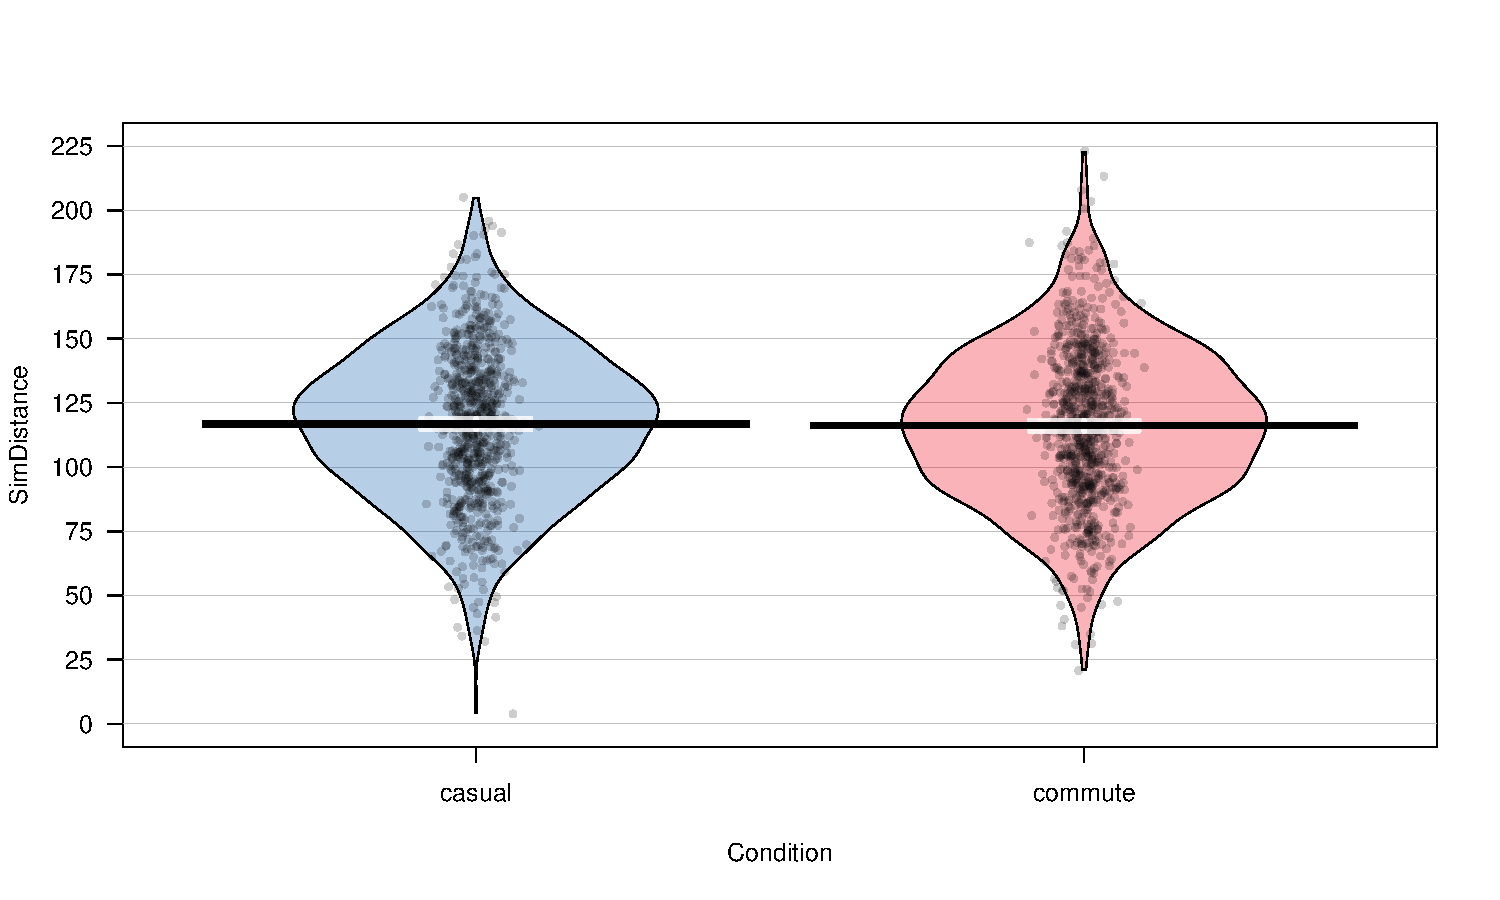
\includegraphics[width=0.75\linewidth]{02-linearmodelsreview_files/figure-latex/Figure2-18-1} 

}

\caption{Pirate-plot of a simulated data set that assumes the same mean for both groups. The means in the two groups are very similar.}\label{fig:Figure2-18}
\end{figure}

\indent The following code chunk generates one run through generating ten data sets as the loop works through the index \texttt{c}, simulates a new set of responses (\texttt{ddsub\$SimDistance}), fits a model that explores the difference in the means of the two groups (\texttt{lm\_sim}), and extracts the ten p-values (stored in \texttt{pval10}) and estimated difference in the means (stored in \texttt{diff10}). The smallest p-value of the ten p-values (\texttt{min(pval10)}) is 0.00576. By finding the value of \texttt{diff10} where \texttt{pval10} is equal to (\texttt{==}) the \texttt{min(pval10)}, the estimated difference in the means from the simulated responses that produced the smallest p-value can be extracted. The difference was -4.17 here. As in the previous initial explorations of permutations, this is just one realization of this process and it needs to be repeated many times to study the impacts of using (1) the first realization of the responses to estimate the difference and p-value and (2) the result with the smallest p-value from ten different realizations of the responses to estimate the difference and p-value. In the following code, we added
octothorpes (\#)\footnote{You can correctly call octothorpes \emph{number} symbols or, in the
  twitter verse, \emph{hashtags}. For more on this symbol, see
  ``\url{http://blog.dictionary.com/octothorpe/}''. Even after reading this, I call them
  number symbols.} and then some text to explain what is being calculated. In computer code, octothorpes
provide a way of adding comments that tell the software (here R) to ignore any
text after a ``\#'' on a given line. In the color version of the text, comments are
even more clearly distinguished.

\begin{Shaded}
\begin{Highlighting}[]
\CommentTok{\# For one iteration through generating 10 data sets:}
\NormalTok{diff10 }\OtherTok{\textless{}{-}}\NormalTok{ pval10 }\OtherTok{\textless{}{-}} \FunctionTok{matrix}\NormalTok{(}\ConstantTok{NA}\NormalTok{, }\AttributeTok{nrow =} \DecValTok{10}\NormalTok{) }\CommentTok{\#Create empty vectors to store 10 results}
\FunctionTok{set.seed}\NormalTok{(}\DecValTok{222}\NormalTok{)}
\CommentTok{\# Create 10 data sets, keep estimated differences and p{-}values in diff10 and pval10}
\ControlFlowTok{for}\NormalTok{ (c }\ControlFlowTok{in}\NormalTok{ (}\DecValTok{1}\SpecialCharTok{:}\DecValTok{10}\NormalTok{))\{}
\NormalTok{  ddsub}\SpecialCharTok{$}\NormalTok{SimDistance }\OtherTok{\textless{}{-}} \FunctionTok{simulate}\NormalTok{(lm\_commonmean)[[}\DecValTok{1}\NormalTok{]]}
  \CommentTok{\# Estimate two group model using simulated responses}
\NormalTok{  lm\_sim }\OtherTok{\textless{}{-}} \FunctionTok{lm}\NormalTok{(SimDistance }\SpecialCharTok{\textasciitilde{}}\NormalTok{ Condition, }\AttributeTok{data =}\NormalTok{ ddsub) }
\NormalTok{  diff10[c] }\OtherTok{\textless{}{-}} \FunctionTok{coef}\NormalTok{(lm\_sim)[}\DecValTok{2}\NormalTok{]}
\NormalTok{  pval10[c] }\OtherTok{\textless{}{-}} \FunctionTok{summary}\NormalTok{(lm\_sim)}\SpecialCharTok{$}\NormalTok{coef[}\DecValTok{2}\NormalTok{,}\DecValTok{4}\NormalTok{]}
\NormalTok{\}}
  
\FunctionTok{tibble}\NormalTok{(pval10, diff10)  }
\end{Highlighting}
\end{Shaded}

\begin{verbatim}
## # A tibble: 10 x 2
##    pval10[,1] diff10[,1]
##         <dbl>      <dbl>
##  1    0.735      -0.492 
##  2    0.326       1.44  
##  3    0.158      -2.06  
##  4    0.265      -1.66  
##  5    0.153       2.09  
##  6    0.00576    -4.17  
##  7    0.915       0.160 
##  8    0.313      -1.50  
##  9    0.983       0.0307
## 10    0.268      -1.69
\end{verbatim}

\begin{Shaded}
\begin{Highlighting}[]
\FunctionTok{min}\NormalTok{(pval10) }\CommentTok{\#Smallest of 10 p{-}values}
\end{Highlighting}
\end{Shaded}

\begin{verbatim}
## [1] 0.005764602
\end{verbatim}

\begin{Shaded}
\begin{Highlighting}[]
\NormalTok{diff10[pval10 }\SpecialCharTok{==} \FunctionTok{min}\NormalTok{(pval10)] }\CommentTok{\#Estimated difference for data set with smallest p{-}value}
\end{Highlighting}
\end{Shaded}

\begin{verbatim}
## [1] -4.170526
\end{verbatim}

\indent In these results, the first data set shows little evidence against the null hypothesis with a p-value of 0.735 and an estimated difference of -0.49. But if you repeat this process and focus just on the ``top'' p-value result, you think that there is moderate evidence against the null hypothesis with a p-value from the sixth data set due to its p-value of 0.0057. Remember that these are all data sets simulated with the null hypothesis being true, so we should not reject the null hypothesis. But we would expect an occasional false detection (Type I error -- rejecting the null hypothesis when it is true) due to sampling variability in the data sets. But by exploring many results and selecting a single result from that suite of results (and not accounting for that selection process in the results), there is a clear issue with exaggerating the strength of evidence. While not obvious yet, we also create an issue with the estimated mean difference in the groups that is demonstrated below.

\indent To fully explore the impacts of either the office drawer or publication bias (they basically have the same impacts on published results even though they are different mechanisms), this process must be repeated many times. The code is a bit more complex here, as the previous code that created ten data sets needs to be replicated \emph{B} = 1,000 times and four sets of results stored (estimated mean differences and p-values for the first data set and the smallest p-value one). This involves a loop that is very similar to our permutation loop but with more activity inside that loop, with the code for generating and extracting the realization of ten results repeated \emph{B} times. Figure \ref{fig:Figure2-19} contains the results for the simulation study. In the left plot that contains the p-values we can immediately see some important differences in the distribution of p-values. In the ``first'' result, the p-values are evenly spread from 0 to 1 -- this is what happens when the null hypothesis is true and you simulate from that scenario one time and track the p-values. A good testing method should make a mistake at the \(\alpha\)-level at a rate around \(\alpha\) (a 5\% significance level test should make a mistake 5\% of the time). If the p-values are evenly spread from 0 to 1, then about 0.05 will be between 0 and 0.05 (think of areas in rectangles with a height of 1 where the total area from 0 to 1 has to add up to 1). But when a researcher focuses only on the top result of ten, then the p-value distribution is smashed toward 0. Using \texttt{favstats} on each distribution of p-values shows that the median for the p-values from taking the first result is around 0.5 but for taking the minimum of ten results, the median p-value is 0.065. So half the results are at the ``moderate'' evidence level or better when selection of results is included. This gets even worse as more results are explored but seems quite problematic here.

\indent The estimated difference in the means also presents an interesting story. When just reporting the first result, the distribution of the estimated means in panel b of Figure \ref{fig:Figure2-19} shows a symmetric distribution that is centered around 0 with results extending just past \(\pm\) 4 in each tail. When selection of results is included, only more extreme estimated differences are considered and no results close to 0 are even reported. There are two modes here around \(\pm\) 2.5 and multiple results close to \(\pm\) 5 are observed. Interestingly, the mean of both distributions is close to 0 so both are ``unbiased'' \footnote{An unbiased estimator \index{unbiased estimator} is a statistic that is on average equal to the population parameter.} estimators but the distribution for the estimated difference from the selected ``top'' result is clearly flawed and would not give correct inferences for differences when the null hypothesis is correct. If a one-sided test had been employed, the selection of the top result would result is a clearly biased estimator as only one of the two modes would be selected. The presentation of these results is a great example of why pirate-plots are better than boxplots as a boxplot of these results would not allow the viewer to notice the two distinct groups of results.



\begin{figure}[ht!]

{\centering 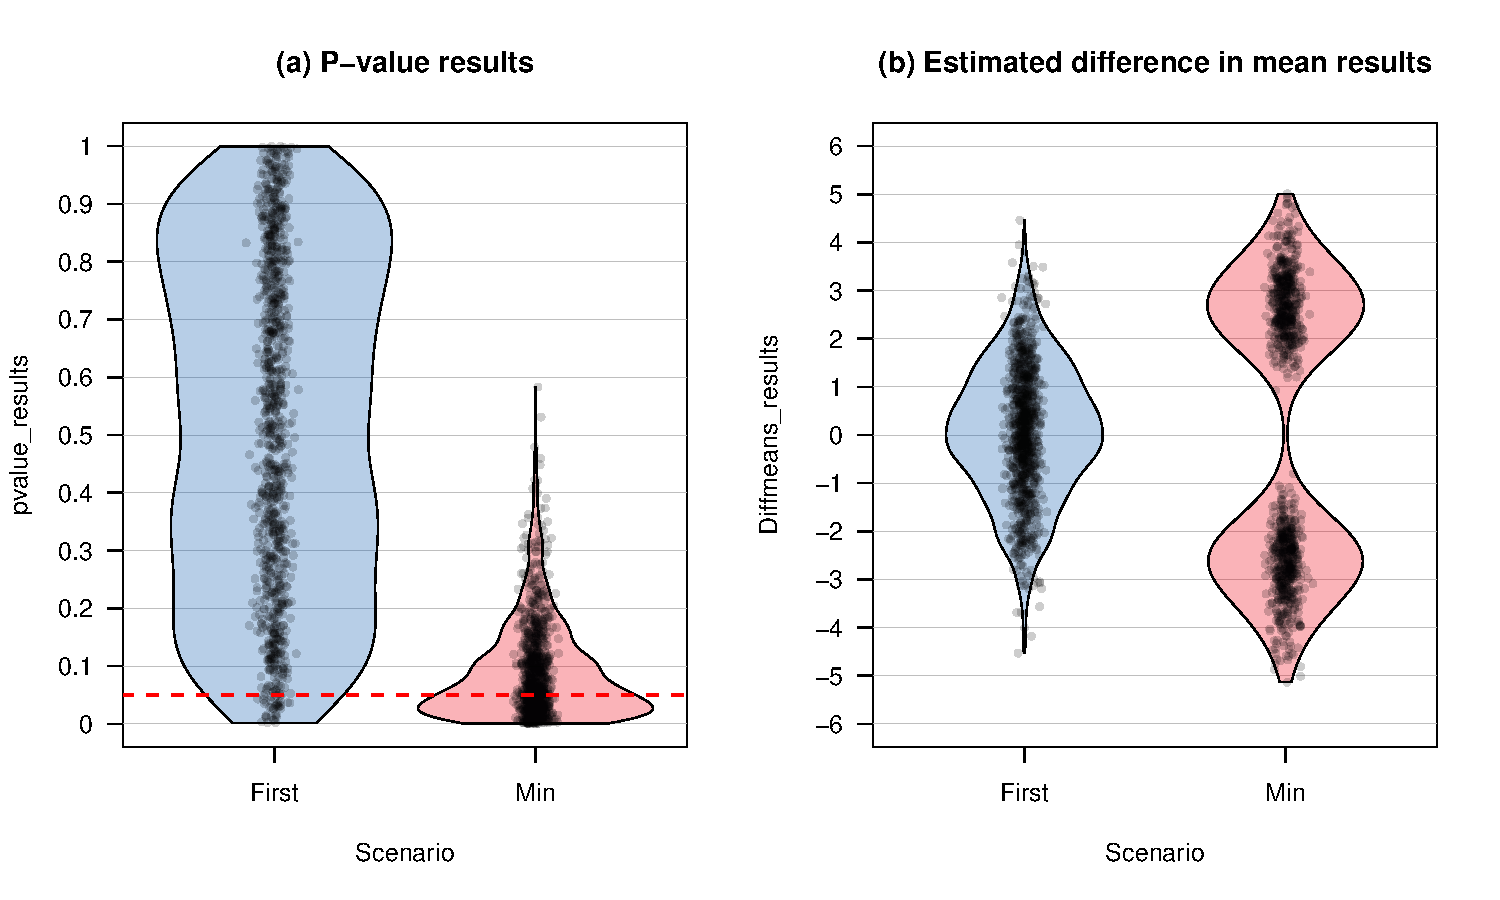
\includegraphics[width=0.75\linewidth]{02-linearmodelsreview_files/figure-latex/Figure2-19-1} 

}

\caption{Pirate-plot of a simulation study results. Panel (a) contains the \emph{B} = 1,000 p-values and (b) contains the \emph{B} = 1,000 estimated differences in the means. Note that the estimated means and confidence intervals normally present in pirate-plots are suppressed here with \texttt{inf.f.o\ =\ 0,\ inf.b.o\ =\ 0,\ avg.line.o\ =\ 0} because these plots are being used to summarize simulation results instead of an original data set.}\label{fig:Figure2-19}
\end{figure}

\newpage

\begin{Shaded}
\begin{Highlighting}[]
\CommentTok{\# Simulation study of generating 10 data sets and either using the first}
\CommentTok{\# or "best p{-}value" result:}
\FunctionTok{set.seed}\NormalTok{(}\DecValTok{1234}\NormalTok{)}

\NormalTok{B }\OtherTok{\textless{}{-}} \DecValTok{1000} \CommentTok{\# \# of simulations}
\CommentTok{\# To store results}
\NormalTok{Diffmeans }\OtherTok{\textless{}{-}}\NormalTok{ pvalues }\OtherTok{\textless{}{-}}\NormalTok{ Diffmeans\_Min }\OtherTok{\textless{}{-}}\NormalTok{ pvalues\_Min }\OtherTok{\textless{}{-}} \FunctionTok{matrix}\NormalTok{(}\ConstantTok{NA}\NormalTok{, }\AttributeTok{nrow =}\NormalTok{ B) }
\ControlFlowTok{for}\NormalTok{ (b }\ControlFlowTok{in}\NormalTok{ (}\DecValTok{1}\SpecialCharTok{:}\NormalTok{B))\{ }\CommentTok{\#Simulation study loop to repeat process B times}
  \CommentTok{\# Create empty vectors to store 10 results for each b}
\NormalTok{  diff10 }\OtherTok{\textless{}{-}}\NormalTok{ pval10 }\OtherTok{\textless{}{-}} \FunctionTok{matrix}\NormalTok{(}\ConstantTok{NA}\NormalTok{, }\AttributeTok{nrow =} \DecValTok{10}\NormalTok{) }
  \ControlFlowTok{for}\NormalTok{ (c }\ControlFlowTok{in}\NormalTok{ (}\DecValTok{1}\SpecialCharTok{:}\DecValTok{10}\NormalTok{))\{ }\CommentTok{\#Loop to create 10 data sets and extract results}
\NormalTok{    ddsub}\SpecialCharTok{$}\NormalTok{SimDistance }\OtherTok{\textless{}{-}} \FunctionTok{simulate}\NormalTok{(lm\_commonmean)[[}\DecValTok{1}\NormalTok{]]}
    \CommentTok{\# Estimate two group model using simulated responses}
\NormalTok{    lm\_sim }\OtherTok{\textless{}{-}} \FunctionTok{lm}\NormalTok{(SimDistance }\SpecialCharTok{\textasciitilde{}}\NormalTok{ Condition, }\AttributeTok{data =}\NormalTok{ ddsub) }
\NormalTok{    diff10[c] }\OtherTok{\textless{}{-}} \FunctionTok{coef}\NormalTok{(lm\_sim)[}\DecValTok{2}\NormalTok{]}
\NormalTok{    pval10[c] }\OtherTok{\textless{}{-}} \FunctionTok{summary}\NormalTok{(lm\_sim)}\SpecialCharTok{$}\NormalTok{coef[}\DecValTok{2}\NormalTok{,}\DecValTok{4}\NormalTok{]}
\NormalTok{  \}}
  
\NormalTok{  pvalues[b] }\OtherTok{\textless{}{-}}\NormalTok{ pval10[}\DecValTok{1}\NormalTok{] }\CommentTok{\#Store first result p{-}value}
\NormalTok{  Diffmeans[b] }\OtherTok{\textless{}{-}}\NormalTok{ diff10[}\DecValTok{1}\NormalTok{] }\CommentTok{\#Store first result estimated difference}
  
\NormalTok{  pvalues\_Min[b] }\OtherTok{\textless{}{-}} \FunctionTok{min}\NormalTok{(pval10) }\CommentTok{\#Store smallest p{-}value}
\NormalTok{  Diffmeans\_Min[b] }\OtherTok{\textless{}{-}}\NormalTok{ diff10[pval10 }\SpecialCharTok{==} \FunctionTok{min}\NormalTok{(pval10)] }\CommentTok{\#Store est. diff of smallest p{-}value}
  
\NormalTok{\}}

\CommentTok{\# Put results together}
\NormalTok{results }\OtherTok{\textless{}{-}} \FunctionTok{tibble}\NormalTok{(}\AttributeTok{pvalue\_results =} \FunctionTok{c}\NormalTok{(pvalues,pvalues\_Min), }
                  \AttributeTok{Diffmeans\_results =} \FunctionTok{c}\NormalTok{(Diffmeans, Diffmeans\_Min), }
                  \AttributeTok{Scenario =} \FunctionTok{rep}\NormalTok{(}\FunctionTok{c}\NormalTok{(}\StringTok{"First"}\NormalTok{, }\StringTok{"Min"}\NormalTok{), }\AttributeTok{each =}\NormalTok{ B))}

\FunctionTok{par}\NormalTok{(}\AttributeTok{mfrow =} \FunctionTok{c}\NormalTok{(}\DecValTok{1}\NormalTok{,}\DecValTok{2}\NormalTok{)) }\CommentTok{\#Plot results}
\FunctionTok{pirateplot}\NormalTok{(pvalue\_results }\SpecialCharTok{\textasciitilde{}}\NormalTok{ Scenario, }\AttributeTok{data =}\NormalTok{ results, }\AttributeTok{inf.f.o =} \DecValTok{0}\NormalTok{, }\AttributeTok{inf.b.o =} \DecValTok{0}\NormalTok{,}
           \AttributeTok{avg.line.o =} \DecValTok{0}\NormalTok{, }\AttributeTok{main =} \StringTok{"(a) P{-}value results"}\NormalTok{)}
\FunctionTok{abline}\NormalTok{(}\AttributeTok{h =} \FloatTok{0.05}\NormalTok{, }\AttributeTok{lwd =} \DecValTok{2}\NormalTok{, }\AttributeTok{col =} \StringTok{"red"}\NormalTok{, }\AttributeTok{lty =} \DecValTok{2}\NormalTok{)}
\FunctionTok{pirateplot}\NormalTok{(Diffmeans\_results }\SpecialCharTok{\textasciitilde{}}\NormalTok{ Scenario, }\AttributeTok{data =}\NormalTok{ results, }\AttributeTok{inf.f.o =} \DecValTok{0}\NormalTok{, }\AttributeTok{inf.b.o =} \DecValTok{0}\NormalTok{,}
           \AttributeTok{avg.line.o =} \DecValTok{0}\NormalTok{, }\AttributeTok{main =} \StringTok{"(b) Estimated difference in mean results"}\NormalTok{)}
\end{Highlighting}
\end{Shaded}

\small

\begin{Shaded}
\begin{Highlighting}[]
\CommentTok{\# Numerical summaries of results}
\FunctionTok{favstats}\NormalTok{(pvalue\_results }\SpecialCharTok{\textasciitilde{}}\NormalTok{ Scenario, }\AttributeTok{data =}\NormalTok{ results)}
\end{Highlighting}
\end{Shaded}

\begin{verbatim}
##   Scenario          min         Q1    median        Q3       max       mean         sd    n missing
## 1    First 0.0017051496 0.27075755 0.5234412 0.7784957 0.9995293 0.51899179 0.28823469 1000       0
## 2      Min 0.0005727895 0.02718018 0.0646370 0.1273880 0.5830232 0.09156364 0.08611836 1000       0
\end{verbatim}

\begin{Shaded}
\begin{Highlighting}[]
\FunctionTok{favstats}\NormalTok{(Diffmeans\_results }\SpecialCharTok{\textasciitilde{}}\NormalTok{ Scenario, }\AttributeTok{data =}\NormalTok{ results)}
\end{Highlighting}
\end{Shaded}

\begin{verbatim}
##   Scenario       min         Q1     median       Q3      max       mean       sd    n missing
## 1    First -4.531864 -0.8424604 0.07360378 1.002228 4.458951 0.05411473 1.392940 1000       0
## 2      Min -5.136510 -2.6857436 1.24042295 2.736930 5.011190 0.03539750 2.874454 1000       0
\end{verbatim}

\normalsize

\newpage

\indent Generally, the challenge in this situation is that if you perform many tests (ten were the focus before) at the same time (instead of just one test), you inflate the
Type I error rate across the tests.
\index{Type I error}
We can define the \textbf{\emph{family-wise error rate}} \index{family-wise error rate}
as the probability that at least one error is made on a set of tests or, more
compactly, Pr(At least 1 error is made) where Pr() is the probability of an
event occurring. The family-wise error is meant to capture the overall
situation in terms of measuring the likelihood of making a mistake if we
consider many tests, each with some chance of making their own mistake, and
focus on how often we make at least one error when we do many tests. A quick
probability calculation shows the magnitude of the problem. If we start with a
5\% significance level test, then Pr(Type I error on one test) = 0.05 and the Pr(no
errors made on one test) = 0.95, by definition. This is our standard hypothesis
testing situation. Now, suppose we have \(m\) independent tests, then

\[\begin{array}{ll}
& \text{Pr(make at least 1 Type I error given all null hypotheses are true)} \\
& = 1 - \text{Pr(no errors made)} \\
& = 1 - 0.95^m.
\end{array}\]

Figure \ref{fig:Figure2-20} shows how the probability of having at least one
false detection grows rapidly with the number of tests, \(m\). The plot stops at 100
tests since it is effectively a 100\% chance of at least one false detection.
It might seem like doing 100 tests is a lot, but, as mentioned before, some researchers consider situations where millions of tests are
considered. Researchers want to make sure that when they report a ``significant'' result that
it is really likely to be a real result and will show up as a difference in the
next data set they collect. Some researchers are now collecting multiple data
sets to use in a single study and using one data set to identify interesting
results and then using a validation or test data set that they withheld from
initial analysis to try to verify that the first results are also present in that
second data set. This also has problems but the only way to develop an understanding of a process is to look across a suite of studies and learn from that accumulation of evidence. This is a good start but needs to be coupled with complete reporting of all results, even those that have p-values larger than 0.05 to avoid the bias identified in the previous simulation study.



\begin{figure}[ht!]

{\centering 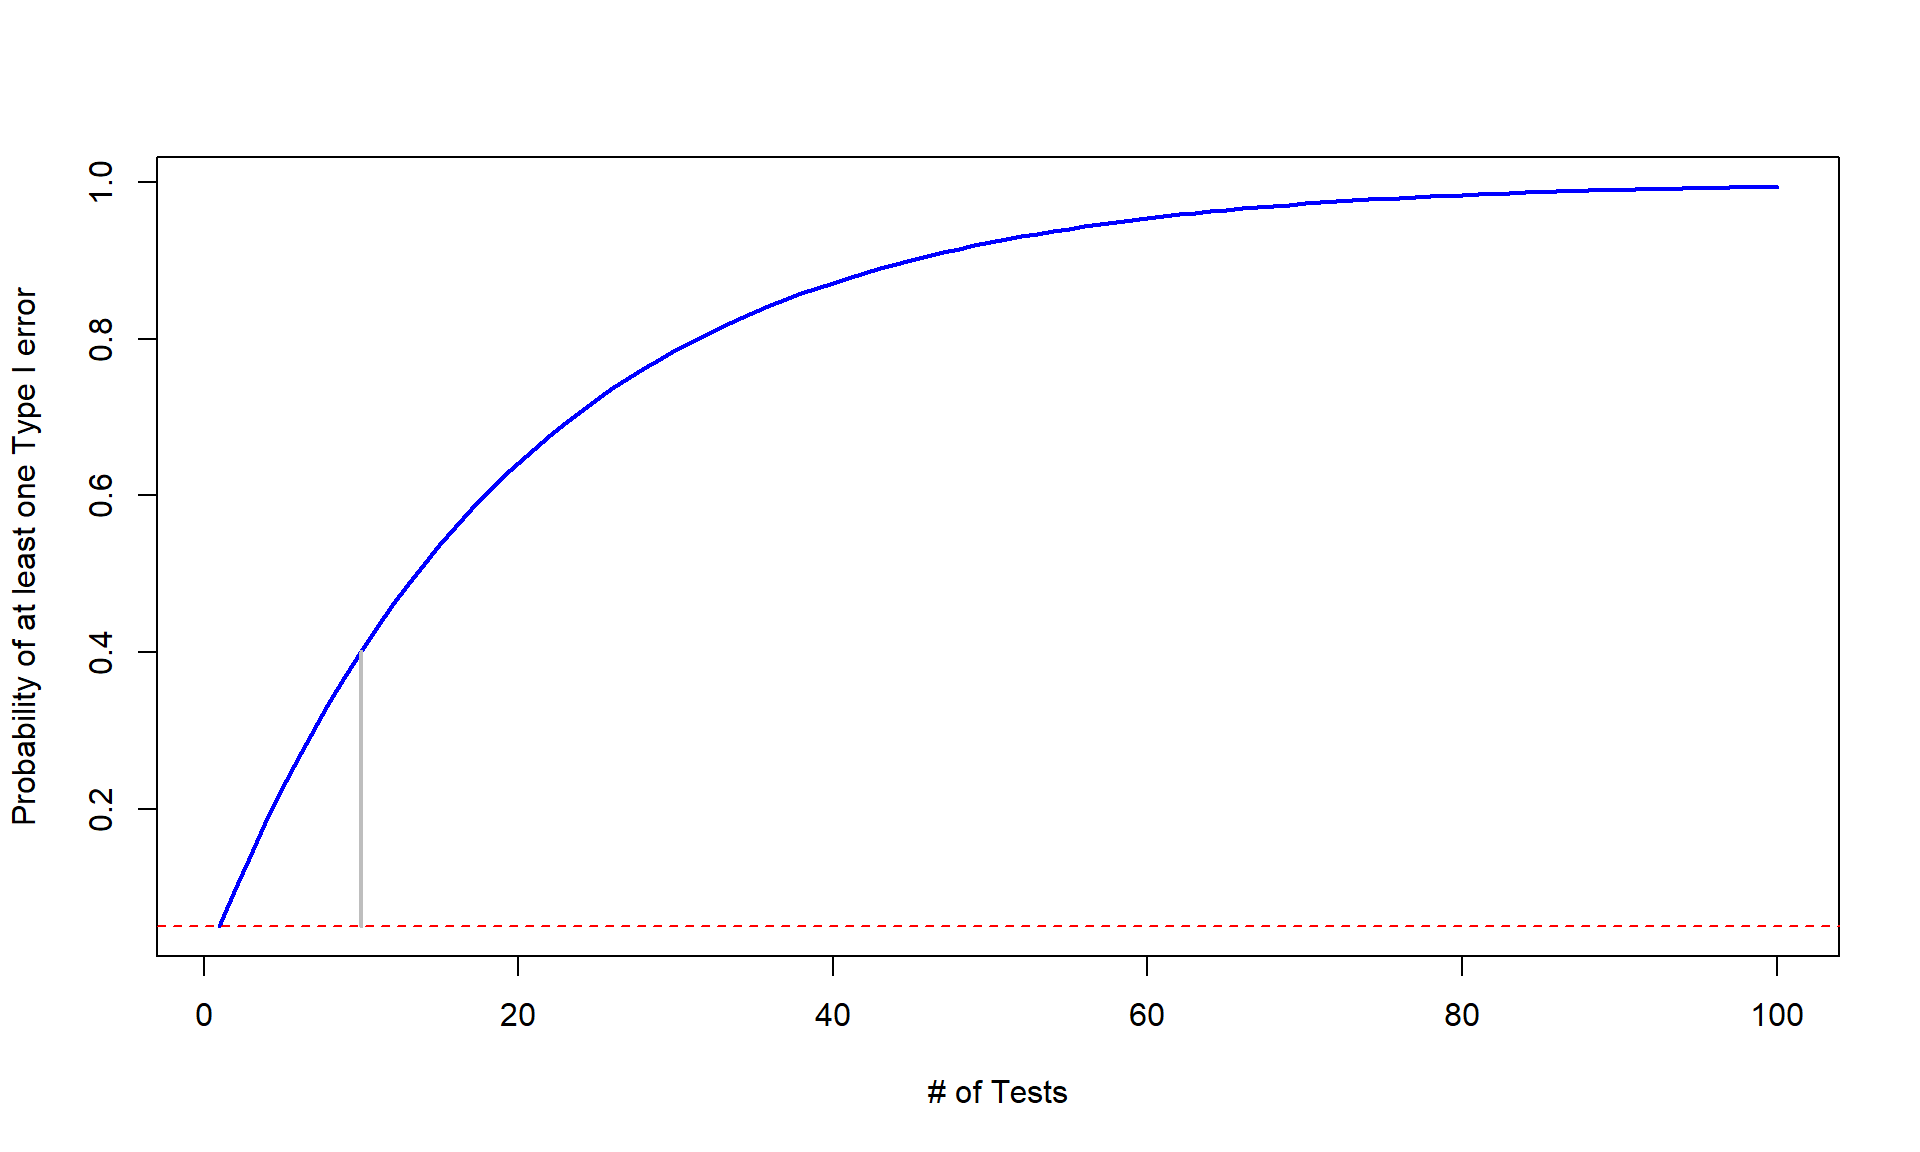
\includegraphics[width=0.75\linewidth]{02-linearmodelsreview_files/figure-latex/Figure2-20-1} 

}

\caption{Plot of family-wise error rate (bold solid line) as the number of tests performed increases. Dashed line indicates 0.05 and grey solid line highlights the probability of at least on error on \(m = 10\) tests.}\label{fig:Figure2-20}
\end{figure}

\indent All hope is not lost when multiple tests are being considered in the same study or by a researcher and exploring more than one result need not lead to clearly biased and flawed results being reported. To account for multiple testing in the same study/analysis, there are many approaches that adjust results to acknowledge that multiple tests are being considered. A simple approach called the ``Bonferroni Correction'' (\protect\hyperlink{ref-Bland1995}{Bland and Altman 1995}) is a good starting point for learning about these methods. It works to control the family-wise error rate of a suite of tests by either dividing \(\alpha\) by the number of tests (\(\alpha/m\)) or, equivalently and more usefully, multiplying the p-value by the number of tests being considered (\(p-value_{adjusted} = p-value \cdot m\) or \(1\) if \(p-value \cdot m > 1\)). The ``Bonferroni adjusted p-values'' are then used as regular p-values to assess evidence against each null hypothesis but now accounting for exploring many of them together. There are some assumptions that this adjustment method makes that make it to generally be a conservative adjustment method. In particular, it assumes that all \(m\) tests are independent of each other and that the null hypothesis was true for all \(m\) tests conducted. While all p-values should be reported in this situation when considering ten results, the impacts of using a Bonferroni correction are that the resulting p-values are not driving inflated Type I error rates even if the smallest p-value is the main focus of the results. The correction also provides a suggestion of decreasing evidence in the first test result because it is now incorporated in considering ten results instead of one.

\indent The following code repeats the simulation study but with the p-values adjusted for multiple testing within each simulation but does not repeat tracking the estimated differences in the means as this is not impacted by the p-value adjustment process. The \texttt{p.adjust} function provides Bonferroni corrections to a vector of p-values (here ten are collected together) using the \texttt{bonferroni} method option (\texttt{p.adjust(pval10,\ method\ =\ "bonferroni")}) and then stores those results. Figure \ref{fig:Figure2-21} shows the results for the first result and minimum result again, but now with these corrections incorporated. The plots may look a bit odd, but in the first data set, so many of the first data sets had p-values that were ``large'' that they were adjusted to have p-values of 1 (so no evidence against the null once we account for multiple testing). The distribution for the minimum p-value results with adjustment more closely resembles the distribution of the first result p-values from Figure \ref{fig:Figure2-19}, except for some minor clumping up at adjusted p-values of 1.



\begin{Shaded}
\begin{Highlighting}[]
\CommentTok{\# Simulation study of generating 10 data sets and either using the first }
\CommentTok{\# or "best p{-}value" result:}
\FunctionTok{set.seed}\NormalTok{(}\DecValTok{1234}\NormalTok{)}

\NormalTok{B }\OtherTok{\textless{}{-}} \DecValTok{1000} \CommentTok{\# \# of simulations}
\NormalTok{pvalues }\OtherTok{\textless{}{-}}\NormalTok{ pvalues\_Min }\OtherTok{\textless{}{-}} \FunctionTok{matrix}\NormalTok{(}\ConstantTok{NA}\NormalTok{, }\AttributeTok{nrow =}\NormalTok{ B) }\CommentTok{\#To store results}
\ControlFlowTok{for}\NormalTok{ (b }\ControlFlowTok{in}\NormalTok{ (}\DecValTok{1}\SpecialCharTok{:}\NormalTok{B))\{ }\CommentTok{\#Simulation study loop to repeat process B times}
  \CommentTok{\# Create empty vectors to store 10 results for each b}
\NormalTok{  pval10 }\OtherTok{\textless{}{-}} \FunctionTok{matrix}\NormalTok{(}\ConstantTok{NA}\NormalTok{, }\AttributeTok{nrow =} \DecValTok{10}\NormalTok{) }
  \ControlFlowTok{for}\NormalTok{ (c }\ControlFlowTok{in}\NormalTok{ (}\DecValTok{1}\SpecialCharTok{:}\DecValTok{10}\NormalTok{))\{ }\CommentTok{\#Loop to create 10 data sets and extract results}
\NormalTok{    ddsub}\SpecialCharTok{$}\NormalTok{SimDistance }\OtherTok{\textless{}{-}} \FunctionTok{simulate}\NormalTok{(lm\_commonmean)[[}\DecValTok{1}\NormalTok{]]}
    \CommentTok{\# Estimate two group model using simulated responses}
\NormalTok{    lm\_sim }\OtherTok{\textless{}{-}} \FunctionTok{lm}\NormalTok{(SimDistance }\SpecialCharTok{\textasciitilde{}}\NormalTok{ Condition, }\AttributeTok{data =}\NormalTok{ ddsub) }
\NormalTok{    pval10[c] }\OtherTok{\textless{}{-}} \FunctionTok{summary}\NormalTok{(lm\_sim)}\SpecialCharTok{$}\NormalTok{coef[}\DecValTok{2}\NormalTok{,}\DecValTok{4}\NormalTok{]}
\NormalTok{  \}}
  
\NormalTok{  pval10 }\OtherTok{\textless{}{-}} \FunctionTok{p.adjust}\NormalTok{(pval10, }\AttributeTok{method =} \StringTok{"bonferroni"}\NormalTok{)}
  
\NormalTok{  pvalues[b] }\OtherTok{\textless{}{-}}\NormalTok{ pval10[}\DecValTok{1}\NormalTok{] }\CommentTok{\#Store first result adjusted p{-}value}
  
\NormalTok{  pvalues\_Min[b] }\OtherTok{\textless{}{-}} \FunctionTok{min}\NormalTok{(pval10) }\CommentTok{\#Store smallest adjusted p{-}value}
\NormalTok{\}}

\CommentTok{\# Put results together}
\NormalTok{results }\OtherTok{\textless{}{-}} \FunctionTok{tibble}\NormalTok{(}\AttributeTok{pvalue\_results =} \FunctionTok{c}\NormalTok{(pvalues, pvalues\_Min), }
                  \AttributeTok{Scenario =} \FunctionTok{rep}\NormalTok{(}\FunctionTok{c}\NormalTok{(}\StringTok{"First"}\NormalTok{, }\StringTok{"Min"}\NormalTok{), }\AttributeTok{each =}\NormalTok{ B))}

\FunctionTok{pirateplot}\NormalTok{(pvalue\_results }\SpecialCharTok{\textasciitilde{}}\NormalTok{ Scenario, }\AttributeTok{data =}\NormalTok{ results, }\AttributeTok{inf.f.o =} \DecValTok{0}\NormalTok{, }\AttributeTok{inf.b.o =} \DecValTok{0}\NormalTok{,}
           \AttributeTok{avg.line.o =} \DecValTok{0}\NormalTok{, }\AttributeTok{main =} \StringTok{"P{-}value results"}\NormalTok{)}
\FunctionTok{abline}\NormalTok{(}\AttributeTok{h =} \FloatTok{0.05}\NormalTok{, }\AttributeTok{lwd =} \DecValTok{2}\NormalTok{, }\AttributeTok{col =} \StringTok{"red"}\NormalTok{, }\AttributeTok{lty =} \DecValTok{2}\NormalTok{)}
\end{Highlighting}
\end{Shaded}

\begin{figure}[ht!]

{\centering 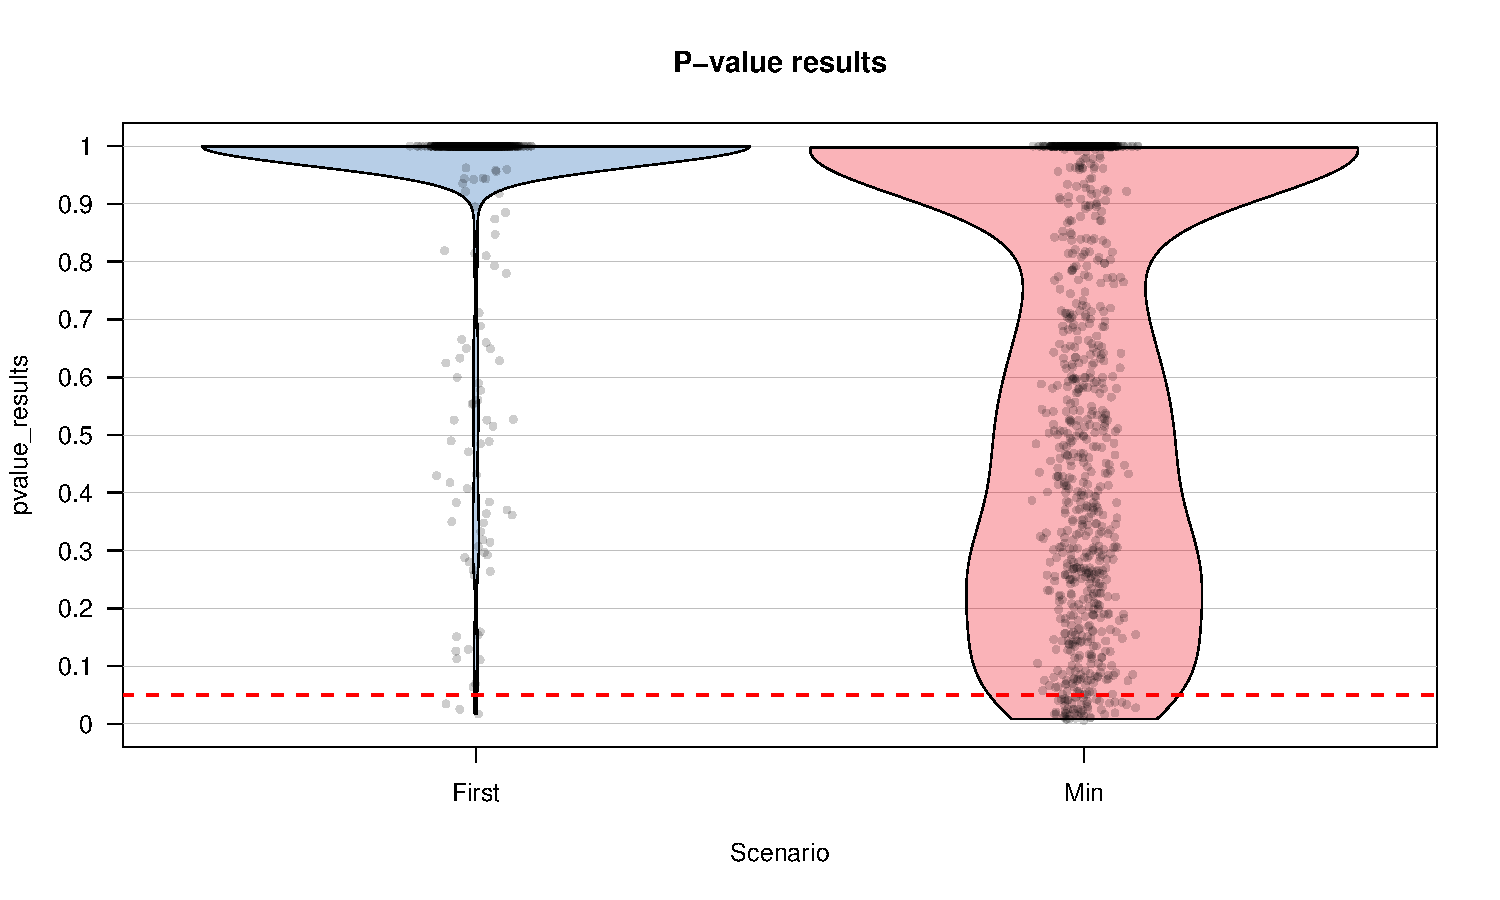
\includegraphics[width=0.75\linewidth]{02-linearmodelsreview_files/figure-latex/Figure2-21-1} 

}

\caption{Pirate-plot of a simulation study results of p-values with Bonferroni correction.}\label{fig:Figure2-21}
\end{figure}

\newpage

By applying the \texttt{pdata} function to the two groups of results, we can directly assess how many of each type (``First'' or ``Min'') resulted in p-values less than 0.05. It ends up that if we adjust for ten tests and just focus on the first result, it is really hard to find moderate or strong evidence against the null hypothesis as only 3 in 1,000 results had adjusted p-values less than 0.05. When the focus is on the ``best'' (or minimum) p-value result when ten are considered and adjustments are made, 52 out of 1,000 results (0.052) show at least moderate evidence against the null hypothesis. This is the rate we would expect from a well-behaved hypothesis test when the null hypothesis is true -- that we would only make a mistake 5\% of the time when \(\alpha\) is 0.05.

\begin{Shaded}
\begin{Highlighting}[]
\CommentTok{\# Numerical summaries of results}
\FunctionTok{favstats}\NormalTok{(pvalue\_results }\SpecialCharTok{\textasciitilde{}}\NormalTok{ Scenario, }\AttributeTok{data =}\NormalTok{ results)}
\end{Highlighting}
\end{Shaded}

\begin{verbatim}
##   Scenario         min        Q1  median Q3 max      mean        sd    n missing
## 1    First 0.017051496 1.0000000 1.00000  1   1 0.9628911 0.1502805 1000       0
## 2      Min 0.005727895 0.2718018 0.64637  1   1 0.6212932 0.3597701 1000       0
\end{verbatim}

\begin{Shaded}
\begin{Highlighting}[]
\CommentTok{\# Proportion of simulations with adjusted p{-}values less than 0.05}
\FunctionTok{pdata}\NormalTok{(pvalue\_results }\SpecialCharTok{\textasciitilde{}}\NormalTok{ Scenario, }\AttributeTok{data =}\NormalTok{ results, .}\DecValTok{05}\NormalTok{, }\AttributeTok{lower.tail =}\NormalTok{ T)}
\end{Highlighting}
\end{Shaded}

\begin{verbatim}
##   Scenario pdata_v
## 1    First   0.003
## 2      Min   0.052
\end{verbatim}

\indent So adjusting for multiple testing is suggested when multiple tests are being considered ``simultaneously''. The Bonferroni adjustment is easy but also crude and can be conservative in applications, especially when the number of tests grows very large (think of multiplying all your p-values by \(m\) = 1,000,000). So other approaches are considered in situations with many tests (there are six other options in the \texttt{p.adjust} function and other functions for doing similar things in R) and there are other approaches that are customized for particular situations with one example discussed in Chapter \ref{chapter3}. The biggest lesson as a statistics student to take from this is that all results are of interest and should be reported and that adjustment of p-values should be considered in studies where many results are being considered. If you are reading results that seem to have walked discretely around these issues you should be suspicious of the real strength of their evidence.

\indent While it wasn't used here, the same general code used to explore this multiple testing issue could be used to explore the power of a particular procedure. If simulations were created from a model with a difference in the means in the groups, then the null hypothesis would have been false and the rate of correctly rejecting the null hypothesis could be studied. The rate of correct rejections is the \emph{power} of a procedure for a chosen version of a true alternative hypothesis (there are many ways to have it be true and you have to choose one to study power) and simply switching the model being simulated from would allow that to be explored. We could also use similar code to compare the power and Type I error rates of parametric versus permutation procedures or to explore situations where an assumption is not true. The steps would be similar -- decide on what you need to simulate from and track a quantity of interest across repeated simulated data sets.

\hypertarget{section2-9}{%
\section{Confidence intervals and bootstrapping}\label{section2-9}}

Up to this point the focus has been on hypotheses, p-values, and estimates of the size of differences. But so far this has not explored inference techniques for the size of the difference. \textbf{\emph{Confidence intervals}} provide an interval where we are \_\_\% \textbf{\emph{confident}} that the true parameter lies. \index{confidence interval} The idea of ``confidence'' is that if we repeated randomly sampling from the same population and made a similar confidence interval, the collection of all these confidence intervals would contain the true parameter at the specified confidence level (usually 95\%). We only get to make one interval and so it either has the true parameter in it or not, and we don't know the truth in real situations.

\indent Confidence intervals can be constructed with parametric \index{parametric} and a
nonparametric approaches. The nonparametric \index{nonparametric}
approach will be using what is
called \textbf{\emph{bootstrapping}}
\index{bootstrap}
and draws its name from ``pull yourself up by
your bootstraps'' where you improve your situation based on your own efforts.
In statistics, we make our situation or inferences better by re-using the
observations we have by assuming that the sample represents the population.
Since each observation represents other similar observations in the
population that we didn't get to measure, if we \textbf{\emph{sample with replacement}}
to generate a new data set of size \emph{n} from our data set (also of size \emph{n})
it mimics the process of taking repeated random samples \index{random sampling} of size \(n\) from our
population of interest. This process also
ends up giving us useful sampling distributions
\index{sampling distribution}
of statistics even when our
standard normality assumption is violated, similar to what we encountered
in the permutation tests. Bootstrapping is especially useful in situations
where we are interested in statistics other than the mean (say we want a
confidence interval for a median or a standard deviation) or when we consider
functions of more than one parameter and don't want to derive the distribution
of the statistic (say the difference in two medians). Here,
bootstrapping is used to provide more trustworthy inferences when some of our
assumptions (especially normality) might be violated for our parametric confidence interval procedure.
\index{assumptions}

\indent To perform bootstrapping, the \texttt{resample} function from the
\texttt{mosaic} package will be used. We can apply this function to a data set and get a new
version of the
data set by sampling new observations \emph{with replacement} from the original one\footnote{Some perform bootstrap sampling in this situation by re-sampling within each of the groups. We will discuss using this technique in situations without clearly defined groups, so prefer to sample with replacement from the entire data set. It also directly corresponds to situations where the data came from one large sample and then the grouping variable of interest was measured on the \(n\) subjects.}.
The new, bootstrapped version of the data set (called \texttt{dsample\_BTS} below)
contains a new variable called \texttt{orig.id} which is the number of the subject
from the original data set. By summarizing how often each of these id's
occurred in a bootstrapped data set, we can see how the re-sampling works.
The \texttt{table} function will count up how many times each observation was used in
the bootstrap sample,
\index{bootstrap!sample}
providing a row with the id followed by a row with the
count\footnote{The \texttt{as.numeric} function is also used here. It really isn't important
  but makes sure the output of \texttt{table} is sorted by observation number by first
  converting the \emph{orig.id} variable into a numeric vector.}. In the first bootstrap
sample shown, the 1\textsuperscript{st}, 14\textsuperscript{th}, and 26\textsuperscript{th} observations
were sampled twice, the 9\textsuperscript{th} and 28\textsuperscript{th} observations were sampled four
times, and the 4\textsuperscript{th}, 5\textsuperscript{th}, 6\textsuperscript{th}, and many others
were not sampled at all. Bootstrap sampling thus picks some observations
multiple times and to do that it has to ignore some\footnote{In any bootstrap sample, about 1/3 of the observations are not used at all.} observations.

\newpage

\begin{Shaded}
\begin{Highlighting}[]
\FunctionTok{set.seed}\NormalTok{(}\DecValTok{406}\NormalTok{)}
\NormalTok{dsample\_BTS }\OtherTok{\textless{}{-}} \FunctionTok{resample}\NormalTok{(dsample)}
\end{Highlighting}
\end{Shaded}

\begin{Shaded}
\begin{Highlighting}[]
\FunctionTok{table}\NormalTok{(}\FunctionTok{as.numeric}\NormalTok{(dsample\_BTS}\SpecialCharTok{$}\NormalTok{orig.id))}
\end{Highlighting}
\end{Shaded}

\begin{verbatim}
## 
##  1  2  3  7  8  9 10 11 12 13 14 16 18 19 23 24 25 26 27 28 30 
##  2  1  1  1  1  4  1  1  1  1  2  1  1  1  1  1  1  2  1  4  1
\end{verbatim}

Like in permutations, one randomization isn't enough. A second bootstrap sample
is also provided to help you get a sense of what bootstrap data sets contain.
It did not select observations two through five but did select eight others more than once.
You can see other variations in the resulting re-sampling of subjects with the
most sampled observation used four times. With \(n = 30\), the chance of
selecting any observation for any slot
in the new data set is \(1/30\) and the expected or mean number of appearances we
expect to see for an observation is the number of random draws times the probably
of selection on each so \(30*1/30 = 1\). So we expect to see each observation in the bootstrap sample on average once but random variability in the samples then creates the possibility of seeing it more than once or not all.

\begin{Shaded}
\begin{Highlighting}[]
\NormalTok{dsample\_BTS2 }\OtherTok{\textless{}{-}} \FunctionTok{resample}\NormalTok{(dsample)}
\FunctionTok{table}\NormalTok{(}\FunctionTok{as.numeric}\NormalTok{(dsample\_BTS2}\SpecialCharTok{$}\NormalTok{orig.id))}
\end{Highlighting}
\end{Shaded}

\begin{verbatim}
## 
##  1  6  7  8  9 10 11 12 13 16 17 20 22 23 24 25 26 28 30 
##  2  2  1  1  2  1  4  1  3  1  1  1  2  2  1  1  2  1  1
\end{verbatim}

We can use the two results to get an idea of distribution of results in terms
of number of times observations might be re-sampled when sampling with
replacement and the variation in those results, as shown in
Figure \ref{fig:Figure2-22}. We could also derive the expected counts for
each number of times of re-sampling when we start with all observations having
an equal chance and sampling with replacement but this isn't important for
using bootstrapping methods.



\begin{figure}[ht!]

{\centering 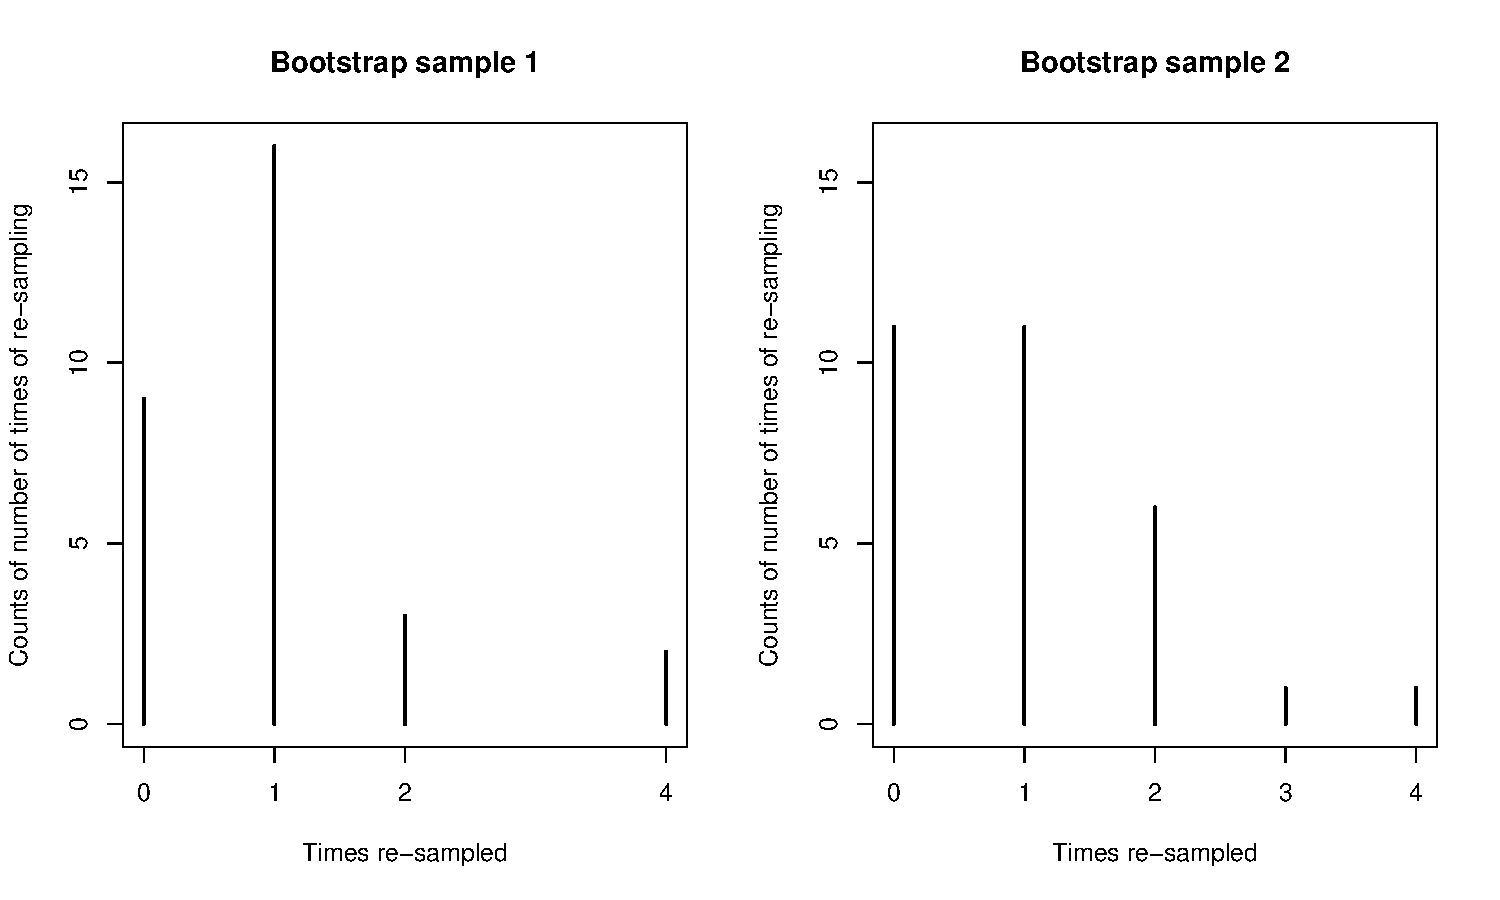
\includegraphics[width=0.75\linewidth]{02-linearmodelsreview_files/figure-latex/Figure2-22-1} 

}

\caption{Counts of number of times of observation (or not observed for times re-sampled of 0) for two bootstrap samples.}\label{fig:Figure2-22}
\end{figure}

\indent The main point of this exploration was to see that each run of the
\texttt{resample} function provides a new version of the data set. Repeating this
\(B\) times using
another \texttt{for} loop, we will track our quantity of interest, say \(T\), in all
these new ``data sets'' and call those results \(T^*\). The distribution of the
bootstrapped
\index{bootstrap!distribution}
\(T^*\) statistics tells us about the range of results to expect
for the statistic. The middle \textbf{\% of the \(T^*\)'s provides a }\%
\textbf{\emph{bootstrap confidence interval}}\footnote{There are actually many ways to use this
  information to make a confidence interval. We are using the simplest method
  that is called the ``percentile'' method.} for the true parameter -- here the \emph{difference in the two population means}.

\indent To make this concrete, we can revisit our previous examples, starting
with the \texttt{dsample} data created before and our interest in comparing the
mean passing distances for the \emph{commuter} and \emph{casual} outfit groups in the \(n = 30\) stratified random sample that was extracted. The
bootstrapping code is very similar to the permutation code except that we apply
the \texttt{resample} function to the entire data set used in \texttt{lm} as opposed to the \texttt{shuffle}
function that was applied only to the explanatory variable.

\begin{Shaded}
\begin{Highlighting}[]
\NormalTok{lm1 }\OtherTok{\textless{}{-}} \FunctionTok{lm}\NormalTok{(Distance }\SpecialCharTok{\textasciitilde{}}\NormalTok{ Condition, }\AttributeTok{data =}\NormalTok{ dsample)}
\NormalTok{Tobs }\OtherTok{\textless{}{-}} \FunctionTok{coef}\NormalTok{(lm1)[}\DecValTok{2}\NormalTok{]; Tobs}
\end{Highlighting}
\end{Shaded}

\begin{verbatim}
## Conditioncommute 
##        -25.93333
\end{verbatim}

\begin{Shaded}
\begin{Highlighting}[]
\NormalTok{B }\OtherTok{\textless{}{-}} \DecValTok{1000}
\FunctionTok{set.seed}\NormalTok{(}\DecValTok{1234}\NormalTok{)}
\NormalTok{Tstar }\OtherTok{\textless{}{-}} \FunctionTok{matrix}\NormalTok{(}\ConstantTok{NA}\NormalTok{, }\AttributeTok{nrow =}\NormalTok{ B)}
\ControlFlowTok{for}\NormalTok{ (b }\ControlFlowTok{in}\NormalTok{ (}\DecValTok{1}\SpecialCharTok{:}\NormalTok{B))\{}
\NormalTok{  lmP }\OtherTok{\textless{}{-}} \FunctionTok{lm}\NormalTok{(Distance }\SpecialCharTok{\textasciitilde{}}\NormalTok{ Condition, }\AttributeTok{data =} \FunctionTok{resample}\NormalTok{(dsample))}
\NormalTok{  Tstar[b] }\OtherTok{\textless{}{-}} \FunctionTok{coef}\NormalTok{(lmP)[}\DecValTok{2}\NormalTok{]}
\NormalTok{\}}
\end{Highlighting}
\end{Shaded}

\begin{Shaded}
\begin{Highlighting}[]
\FunctionTok{favstats}\NormalTok{(Tstar)}
\end{Highlighting}
\end{Shaded}

\begin{verbatim}
##        min        Q1    median        Q3      max      mean       sd    n missing
##  -66.96429 -34.57159 -25.65881 -17.12391 17.17857 -25.73641 12.30987 1000       0
\end{verbatim}



\begin{figure}[ht!]

{\centering 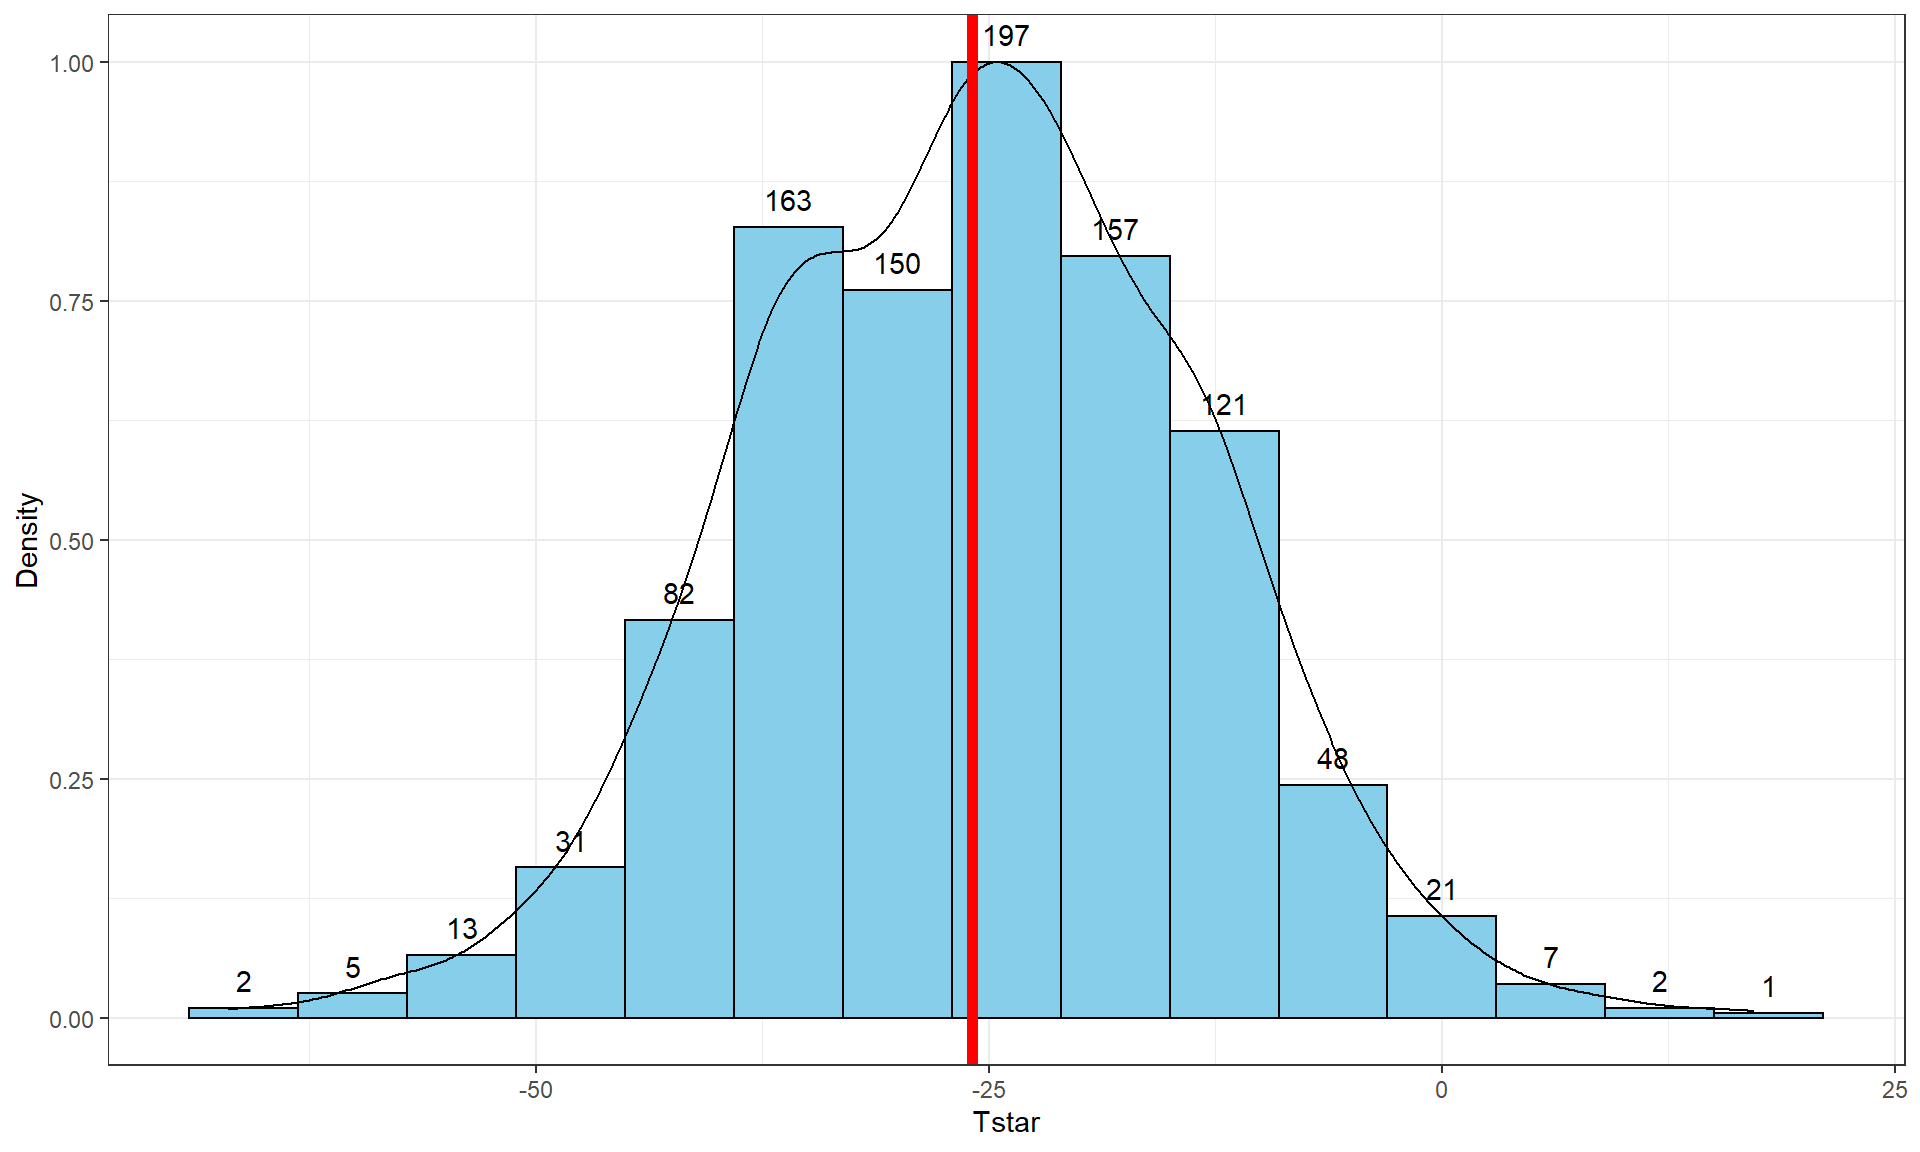
\includegraphics[width=0.75\linewidth]{02-linearmodelsreview_files/figure-latex/Figure2-23-1} 

}

\caption{Histogram and density curve of bootstrap distributions of difference in sample mean \texttt{Distances} with vertical line for the observed difference in the means of -25.933.}\label{fig:Figure2-23}
\end{figure}

\begin{Shaded}
\begin{Highlighting}[]
\FunctionTok{tibble}\NormalTok{(Tstar) }\SpecialCharTok{\%\textgreater{}\%} \FunctionTok{ggplot}\NormalTok{(}\FunctionTok{aes}\NormalTok{(}\AttributeTok{x =}\NormalTok{ Tstar)) }\SpecialCharTok{+} 
  \FunctionTok{geom\_histogram}\NormalTok{(}\FunctionTok{aes}\NormalTok{(}\AttributeTok{y =}\NormalTok{ ..ncount..), }\AttributeTok{bins =} \DecValTok{15}\NormalTok{, }\AttributeTok{col =} \DecValTok{1}\NormalTok{, }\AttributeTok{fill =} \StringTok{"skyblue"}\NormalTok{, }\AttributeTok{center =} \DecValTok{0}\NormalTok{) }\SpecialCharTok{+} 
  \FunctionTok{geom\_density}\NormalTok{(}\FunctionTok{aes}\NormalTok{(}\AttributeTok{y =}\NormalTok{ ..scaled..)) }\SpecialCharTok{+}
  \FunctionTok{theme\_bw}\NormalTok{() }\SpecialCharTok{+}
  \FunctionTok{labs}\NormalTok{(}\AttributeTok{y =} \StringTok{"Density"}\NormalTok{) }\SpecialCharTok{+}
  \FunctionTok{geom\_vline}\NormalTok{(}\AttributeTok{xintercept =}\NormalTok{ Tobs, }\AttributeTok{col =} \StringTok{"red"}\NormalTok{, }\AttributeTok{lwd =} \DecValTok{2}\NormalTok{) }\SpecialCharTok{+}
  \FunctionTok{stat\_bin}\NormalTok{(}\FunctionTok{aes}\NormalTok{(}\AttributeTok{y =}\NormalTok{ ..ncount.., }\AttributeTok{label =}\NormalTok{ ..count..), }\AttributeTok{bins =} \DecValTok{15}\NormalTok{, }
           \AttributeTok{geom =} \StringTok{"text"}\NormalTok{, }\AttributeTok{vjust =} \SpecialCharTok{{-}}\FloatTok{0.75}\NormalTok{)}
\end{Highlighting}
\end{Shaded}

In this situation, the observed difference in the mean passing distances is -25.933 cm
(\emph{commute} - \emph{casual}), which is the bold vertical line in Figure
\ref{fig:Figure2-23}.
The bootstrap distribution
\index{bootstrap!distribution}
shows the results for the difference in the sample
means when fake data sets are re-constructed by sampling from the original data set with
replacement. The bootstrap distribution is approximately centered at the observed
value (difference in the sample means) and is relatively symmetric.

\indent The permutation distribution \index{permutation!distribution} in the same situation (Figure
\ref{fig:Figure2-10}) had a similar shape but was centered at 0.
Permutations create sampling
distributions
\index{sampling distribution}
based on assuming the null hypothesis is true, which is useful for
hypothesis testing. Bootstrapping creates distributions centered at the observed
result, which is the sampling distribution ``under the alternative'' or when no null
hypothesis is assumed; bootstrap distributions are useful for generating
confidence intervals for the true parameter values.

\indent To create a 95\% bootstrap confidence interval for the difference in
the true mean distances (\(\mu_\text{commute}-\mu_\text{casual}\)), select the
middle 95\% of results from
the bootstrap distribution. Specifically, find the 2.5\textsuperscript{th}
percentile and the 97.5\textsuperscript{th} percentile (values that put 2.5 and 97.5\%
of the results to the left) in the bootstrap distribution, which leaves 95\% in
the middle for the confidence interval. To find percentiles in a distribution
in R, functions are of the form \texttt{q{[}Name\ of\ distribution{]}}, with the function
\texttt{qt} extracting percentiles from a \(t\)-distribution (examples below). From the
bootstrap results, use the \texttt{qdata} function on the \texttt{Tstar} results that
contain the bootstrap distribution of the statistic of interest.

\begin{Shaded}
\begin{Highlighting}[]
\FunctionTok{qdata}\NormalTok{(Tstar, }\FloatTok{0.025}\NormalTok{)}
\end{Highlighting}
\end{Shaded}

\begin{verbatim}
##     2.5% 
## -50.0055
\end{verbatim}

\begin{Shaded}
\begin{Highlighting}[]
\FunctionTok{qdata}\NormalTok{(Tstar, }\FloatTok{0.975}\NormalTok{)}
\end{Highlighting}
\end{Shaded}

\begin{verbatim}
##     97.5% 
## -2.248774
\end{verbatim}

These results tell us that the 2.5\textsuperscript{th} percentile of the bootstrap
distribution is at -50.006 cm and the 97.5\textsuperscript{th} percentile is at -2.249 cm. We can combine these results to provide a 95\% confidence for
\(\mu_\text{commute}-\mu_\text{casaual}\) that is between -50.01 and -2.25 cm. This interval is interpreted as with any confidence interval, that we are 95\% confident that the difference
in the true mean distances (\emph{commute} minus \emph{casual} groups) is
between -50.01 and -2.25 cm. Or we can switch the direction of the comparison and say that we are 95\% confident that the difference in the true means is between 2.25 and 50.01 cm (\emph{casual} minus \emph{commute}). This result would be incorporated into step 5 of the hypothesis testing protocol to accompany discussing the size of the estimated difference in the groups or used as a result of interest in itself. Both percentiles can be obtained in one line
of code using:

\begin{Shaded}
\begin{Highlighting}[]
\NormalTok{quantiles }\OtherTok{\textless{}{-}} \FunctionTok{qdata}\NormalTok{(Tstar, }\FunctionTok{c}\NormalTok{(}\FloatTok{0.025}\NormalTok{,}\FloatTok{0.975}\NormalTok{))}
\end{Highlighting}
\end{Shaded}

\begin{Shaded}
\begin{Highlighting}[]
\NormalTok{quantiles}
\end{Highlighting}
\end{Shaded}

\begin{verbatim}
##       2.5%      97.5% 
## -50.005502  -2.248774
\end{verbatim}

Figure \ref{fig:Figure2-24} displays those same percentiles on the bootstrap distribution residing in \texttt{Tstar}.



\begin{figure}[ht!]

{\centering 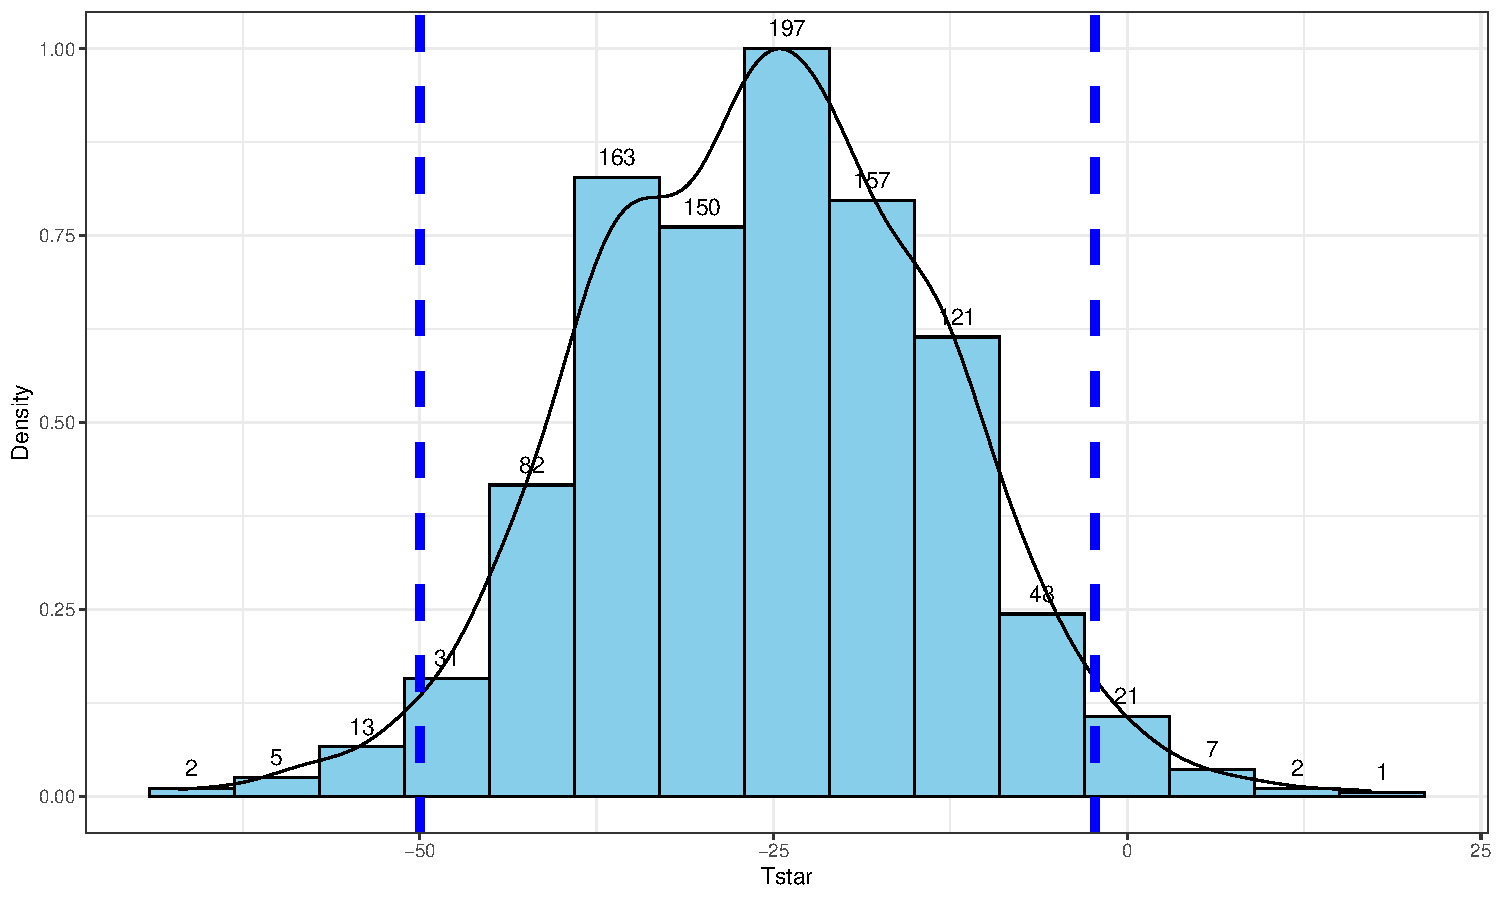
\includegraphics[width=0.75\linewidth]{02-linearmodelsreview_files/figure-latex/Figure2-24-1} 

}

\caption{Histogram and density curve of bootstrap distribution with 95\% bootstrap confidence intervals displayed (bold, dashed vertical lines).}\label{fig:Figure2-24}
\end{figure}

\begin{Shaded}
\begin{Highlighting}[]
\FunctionTok{tibble}\NormalTok{(Tstar) }\SpecialCharTok{\%\textgreater{}\%} \FunctionTok{ggplot}\NormalTok{(}\FunctionTok{aes}\NormalTok{(}\AttributeTok{x =}\NormalTok{ Tstar)) }\SpecialCharTok{+} 
  \FunctionTok{geom\_histogram}\NormalTok{(}\FunctionTok{aes}\NormalTok{(}\AttributeTok{y =}\NormalTok{ ..ncount..), }\AttributeTok{bins =} \DecValTok{15}\NormalTok{, }\AttributeTok{col =} \DecValTok{1}\NormalTok{, }\AttributeTok{fill =} \StringTok{"skyblue"}\NormalTok{, }\AttributeTok{center =} \DecValTok{0}\NormalTok{) }\SpecialCharTok{+} 
  \FunctionTok{geom\_density}\NormalTok{(}\FunctionTok{aes}\NormalTok{(}\AttributeTok{y =}\NormalTok{ ..scaled..)) }\SpecialCharTok{+}
  \FunctionTok{theme\_bw}\NormalTok{() }\SpecialCharTok{+}
  \FunctionTok{labs}\NormalTok{(}\AttributeTok{y =} \StringTok{"Density"}\NormalTok{) }\SpecialCharTok{+}
  \FunctionTok{geom\_vline}\NormalTok{(}\AttributeTok{xintercept =}\NormalTok{ quantiles, }\AttributeTok{col =} \StringTok{"blue"}\NormalTok{, }\AttributeTok{lwd =} \DecValTok{2}\NormalTok{, }\AttributeTok{lty =} \DecValTok{2}\NormalTok{) }\SpecialCharTok{+}
  \FunctionTok{stat\_bin}\NormalTok{(}\FunctionTok{aes}\NormalTok{(}\AttributeTok{y =}\NormalTok{ ..ncount.., }\AttributeTok{label =}\NormalTok{ ..count..), }\AttributeTok{bins =} \DecValTok{15}\NormalTok{, }
           \AttributeTok{geom =} \StringTok{"text"}\NormalTok{, }\AttributeTok{vjust =} \SpecialCharTok{{-}}\FloatTok{0.75}\NormalTok{)}
\end{Highlighting}
\end{Shaded}

\indent Although confidence intervals can exist without referencing hypotheses,
we can
revisit our previous hypotheses and see what this confidence interval tells
us about the test of \(H_0: \mu_\text{commute} = \mu_\text{casual}\). This null
hypothesis is equivalent to testing \(H_0: \mu_\text{commute} - \mu_\text{casual} = 0\),
that the difference
in the true means is equal to 0 cm. And the difference in the means was the
scale for our confidence interval, which did not contain 0 cm. The
0 cm values is an interesting \textbf{\emph{reference value}} for the confidence interval, because
here it is the value where the true means are equal to each other (have a
difference of 0 cm). In general, if our confidence interval does not contain
0, then it is saying that 0 is not one of the likely values for the difference
in the true means at the selected confidence level. This implies that we should reject a claim that they are
equal. This provides the same inferences for the hypotheses that we considered
previously using both parametric and permutation approaches using a fixed \(\alpha\) approach where \(\alpha\) = 1 - confidence level.

\indent The general summary
is that we can use confidence intervals to test hypotheses by assessing whether
the reference value under the null hypothesis is in the confidence interval
(suggests insufficient evidence against \(H_0\) to reject it, at least at the \(\alpha\) level and equivalent to having a p-value larger than \(\alpha\)) or outside the confidence interval (sufficient evidence against \(H_0\) to reject it and equivalent to having a p-value that is less than \(\alpha\)). P-values
\index{p-value}
are more
informative about hypotheses (measure of evidence against the null hypothesis)
but confidence intervals are more informative
about the size of differences, so both offer useful information and, as shown
here, can provide consistent conclusions about hypotheses. But it is best practice to use p-values to assess evidence against null hypotheses and confidence intervals to do inferences for the size of differences.

\indent As in the previous situation, we also want to consider the parametric
approach
for comparison purposes and to have that method available, especially to help
us understand some methods where we will only consider parametric inferences
in later chapters. The parametric confidence interval is called the
\textbf{\emph{equal variance, two-sample t confidence interval}} and additionally
assumes that the populations
being sampled from are normally distributed instead of just that they have similar shapes in the bootstrap approach. The parametric method leads to using a \(t\)-distribution
\index{@$t$-distribution}
to form the interval with the degrees of freedom for the \(t\)-distribution of \(n-2\) although we can obtain it without direct reference to this distribution using the \texttt{confint} function applied to the \texttt{lm} model. This function generates two confidence intervals and the one in the second row is the one we are interested as it pertains to the difference in the true means of the two groups. The parametric 95\% confidence interval here is from -51.6 to -0.26 cm which is a bit different in width from the nonparametric bootstrap interval that was from -50.01 and -2.25 cm.

\begin{Shaded}
\begin{Highlighting}[]
\FunctionTok{confint}\NormalTok{(lm1)}
\end{Highlighting}
\end{Shaded}

\begin{verbatim}
##                      2.5 %      97.5 %
## (Intercept)      117.64498 153.9550243
## Conditioncommute -51.60841  -0.2582517
\end{verbatim}

The bootstrap interval was narrower by almost 4 cm and its upper limit was much further from 0. The bootstrap CI can vary depending on the random number seed used and additional runs of the code produced intervals of (-49.6, -2.8), (-48.3, -2.5), and (-50.9, -1.1) so the differences between the parametric and nonparametric approaches was not just due to an unusual bootstrap distribution. It is not entirely clear why the two intervals differ but there are slightly more results in the left tail of Figure \ref{fig:Figure2-24} than in the right tail and this shifts the 95\% confidence slightly away from 0 as compared to the parametric approach. All intervals have the same interpretation, only the methods for calculating the
intervals and the assumptions differ. Specifically, the bootstrap interval can
tolerate different distribution shapes other than normal and still provide
intervals that work well\footnote{When hypothesis tests ``work well'' they have high
  power \index{power} to detect differences while having Type I error rates \index{Type I error} that are close
  to what we choose \emph{a priori}. When confidence intervals ``work well'', they contain
  the true parameter value in repeated random samples at around the selected
  confidence level, which is called the \textbf{\emph{coverage rate}}. \index{coverage rate}}. The other assumptions
\index{assumptions}
are all the same as for the hypothesis
test, where we continue to assume that we have independent observations with
equal variances for the two groups and maintain concerns about inferences here due to the violation of independence in these responses.

\indent The formula that \texttt{lm} is using to calculate the parametric
\textbf{\emph{equal variance, two-sample \(t\)-based confidence interval}} is:

\[\bar{x}_1 - \bar{x}_2 \mp t^*_{df}s_p\sqrt{\frac{1}{n_1}+\frac{1}{n_2}}\]

In this situation, the \emph{df} is again \(n_1+n_2-2\) (the total sample size - 2) and
\(s_p = \sqrt{\frac{(n_1-1)s_1^2 + (n_2-1)s_2^2}{n_1+n_2-2}}\). The \(t^*_{df}\) is
a multiplier that comes from finding the percentile from the \(t\)-distribution
that puts \(C\)\% in the middle of the distribution with \(C\) being the confidence
level. It is important to note that this \(t^*\) has nothing to do with the previous
test statistic \(t\). It is confusing and students first engaging these two options often happily
take the result from a test statistic calculation and use it for a multiplier
in a \(t\)-based confidence interval -- try to focus on which \(t\) you are interested in before you use either. Figure \ref{fig:Figure2-25} shows the
\(t\)-distribution with 28 degrees of freedom and the cut-offs that put 95\% of the
area in the middle.



\begin{figure}[ht!]

{\centering 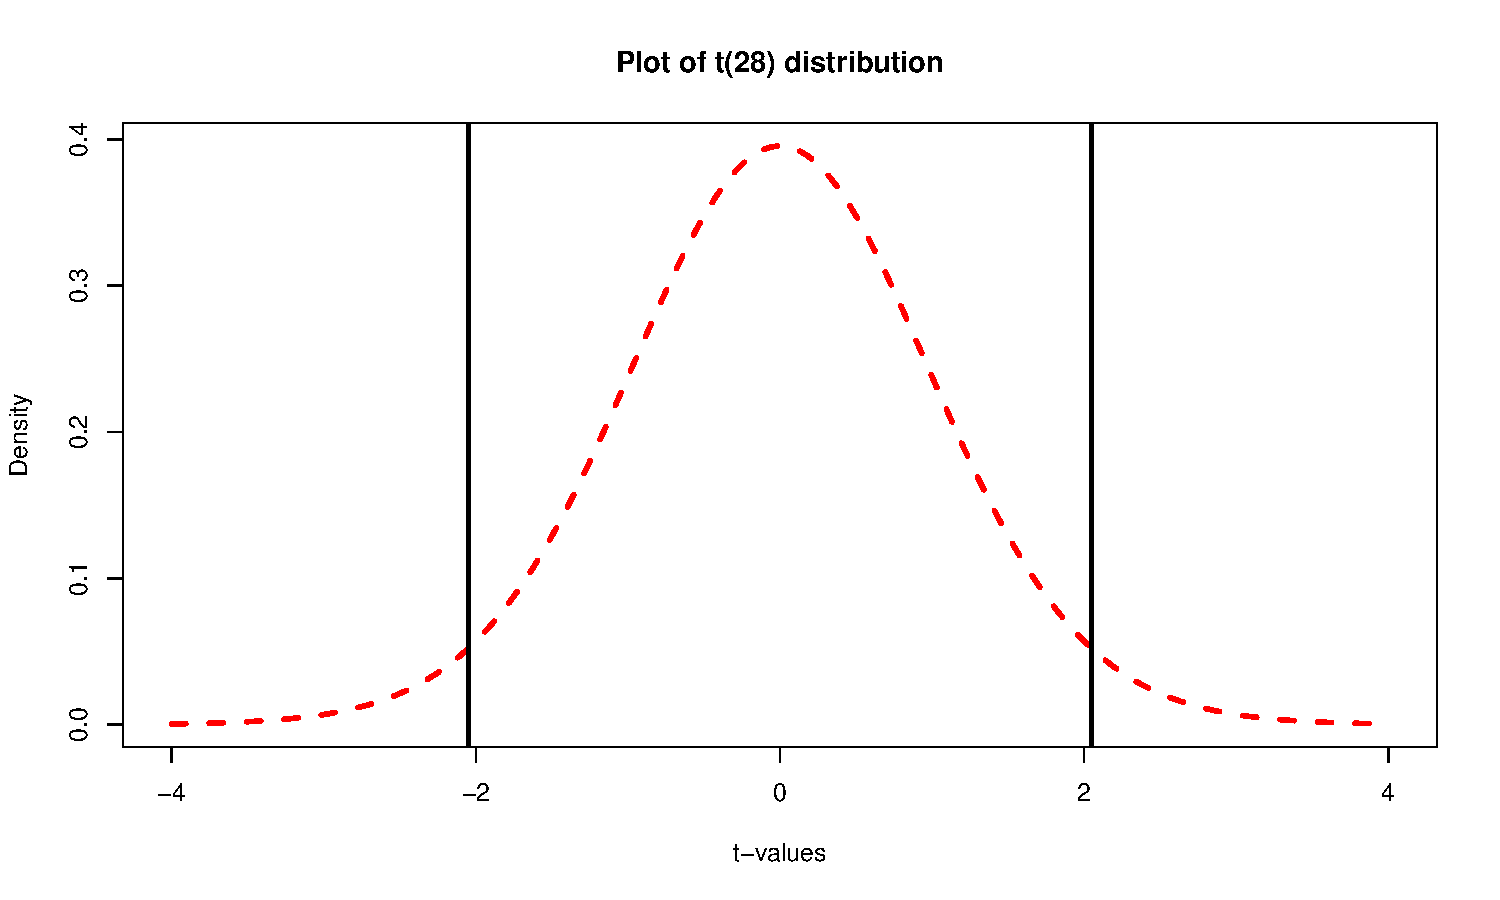
\includegraphics[width=0.75\linewidth]{02-linearmodelsreview_files/figure-latex/Figure2-25-1} 

}

\caption{Plot of \(t(28)\) with cut-offs for putting 95\% of distribution in the middle that delineate the \(t^*\) multiplier to make a 95\% confidence interval.}\label{fig:Figure2-25}
\end{figure}

For 95\% confidence intervals, the multiplier is going to be close to 2 and
anything else is a likely indication of a mistake. We can use R to get the multipliers for
confidence intervals using the \texttt{qt} function in a similar fashion to how
\texttt{qdata} was used in the bootstrap results, except that this new value must be
used in the previous confidence interval formula. This function produces values
for requested percentiles, so if we want to put 95\% in the middle, we place
2.5\% in each tail of the distribution and need to request the 97.5\textsuperscript{th}
percentile. Because the \(t\)-distribution is always symmetric around 0, we merely
need to look up the value for the 97.5\textsuperscript{th} percentile and know that the
multiplier for the 2.5\textsuperscript{th} percentile is just \(-t^*\). The \(t^*\)
multiplier to form the confidence interval is 2.0484 for a 95\% confidence interval
when the \(df = 28\) based on the results from \texttt{qt}:

\begin{Shaded}
\begin{Highlighting}[]
\FunctionTok{qt}\NormalTok{(}\FloatTok{0.975}\NormalTok{, }\AttributeTok{df =} \DecValTok{28}\NormalTok{)}
\end{Highlighting}
\end{Shaded}

\begin{verbatim}
## [1] 2.048407
\end{verbatim}

Note that the 2.5\textsuperscript{th} percentile is just the negative of this value due
to symmetry and the real source of the minus in the minus/plus in the formula
for the confidence interval.

\begin{Shaded}
\begin{Highlighting}[]
\FunctionTok{qt}\NormalTok{(}\FloatTok{0.025}\NormalTok{, }\AttributeTok{df =} \DecValTok{28}\NormalTok{)}
\end{Highlighting}
\end{Shaded}

\begin{verbatim}
## [1] -2.048407
\end{verbatim}

We can also re-write the confidence interval formula into a slightly more
general forms as

\[\bar{x}_1 - \bar{x}_2 \mp t^*_{df}SE_{\bar{x}_1 - \bar{x}_2}\ \text{ OR }\ 
\bar{x}_1 - \bar{x}_2 \mp ME\]

where \(SE_{\bar{x}_1 - \bar{x}_2} = s_p\sqrt{\frac{1}{n_1}+\frac{1}{n_2}}\) and
\(ME = t^*_{df}SE_{\bar{x}_1 - \bar{x}_2}\). The \emph{SE} is available in the \texttt{lm} model \texttt{summary} for the line related to the difference in groups in the ``Std. Error'' column. In some situations, researchers will
report the \textbf{\emph{standard error}} (SE) or \textbf{\emph{margin of error}} (ME) as a method
of quantifying the uncertainty in a statistic. The SE is an estimate of the
standard deviation of the statistic (here \(\bar{x}_1 - \bar{x}_2\)) and the ME
is an estimate of the precision of a statistic that can be used to directly
form a confidence interval. The ME depends on the choice of confidence level
although 95\% is almost always selected.

\indent To finish this example, R can be used to help you do calculations much
like a calculator except with much more power ``under the hood''. You have to
make sure you are careful with using \texttt{(\ )} to group items and remember that
the asterisk (*) is used for multiplication. We need the pertinent
information which is available from the \texttt{favstats} output repeated below to
calculate the confidence interval ``by hand''\footnote{We will often use this term to
  indicate perform a calculation using the \texttt{favstats} results -- not that you need to go back to
  the data set and calculate the means and standard deviations yourself.} using R.

\begin{Shaded}
\begin{Highlighting}[]
\FunctionTok{favstats}\NormalTok{(Distance }\SpecialCharTok{\textasciitilde{}}\NormalTok{ Condition, }\AttributeTok{data =}\NormalTok{ dsample)}
\end{Highlighting}
\end{Shaded}

\begin{verbatim}
##   Condition min    Q1 median    Q3 max     mean       sd  n missing
## 1    casual  72 112.5    143 154.5 208 135.8000 39.36133 15       0
## 2   commute  60  88.5    113 123.0 168 109.8667 28.41244 15       0
\end{verbatim}

Start with typing the following command to calculate \(s_p\) and store it in a
variable named \texttt{sp}:

\begin{Shaded}
\begin{Highlighting}[]
\NormalTok{sp }\OtherTok{\textless{}{-}} \FunctionTok{sqrt}\NormalTok{(((}\DecValTok{15} \SpecialCharTok{{-}} \DecValTok{1}\NormalTok{)}\SpecialCharTok{*}\NormalTok{(}\FloatTok{39.36133}\SpecialCharTok{\^{}}\DecValTok{2}\NormalTok{) }\SpecialCharTok{+}\NormalTok{ (}\DecValTok{15} \SpecialCharTok{{-}} \DecValTok{1}\NormalTok{)}\SpecialCharTok{*}\NormalTok{(}\FloatTok{28.4124}\SpecialCharTok{\^{}}\DecValTok{2}\NormalTok{))}\SpecialCharTok{/}\NormalTok{(}\DecValTok{15} \SpecialCharTok{+} \DecValTok{15} \SpecialCharTok{{-}} \DecValTok{2}\NormalTok{))}
\NormalTok{sp}
\end{Highlighting}
\end{Shaded}

\begin{verbatim}
## [1] 34.32622
\end{verbatim}

Then calculate the confidence interval that \texttt{confint} provided using:

\begin{Shaded}
\begin{Highlighting}[]
\FloatTok{109.8667} \SpecialCharTok{{-}} \FloatTok{135.8} \SpecialCharTok{+} \FunctionTok{c}\NormalTok{(}\SpecialCharTok{{-}}\DecValTok{1}\NormalTok{,}\DecValTok{1}\NormalTok{)}\SpecialCharTok{*}\FunctionTok{qt}\NormalTok{(}\FloatTok{0.975}\NormalTok{, }\AttributeTok{df =} \DecValTok{28}\NormalTok{)}\SpecialCharTok{*}\NormalTok{sp}\SpecialCharTok{*}\FunctionTok{sqrt}\NormalTok{(}\DecValTok{1}\SpecialCharTok{/}\DecValTok{15} \SpecialCharTok{+} \DecValTok{1}\SpecialCharTok{/}\DecValTok{15}\NormalTok{)}
\end{Highlighting}
\end{Shaded}

\begin{verbatim}
## [1] -51.6083698  -0.2582302
\end{verbatim}

Or using the information from the model summary:

\begin{Shaded}
\begin{Highlighting}[]
\SpecialCharTok{{-}}\FloatTok{25.933} \SpecialCharTok{+} \FunctionTok{c}\NormalTok{(}\SpecialCharTok{{-}}\DecValTok{1}\NormalTok{,}\DecValTok{1}\NormalTok{)}\SpecialCharTok{*}\FunctionTok{qt}\NormalTok{(}\FloatTok{0.975}\NormalTok{, }\AttributeTok{df =} \DecValTok{28}\NormalTok{)}\SpecialCharTok{*}\FloatTok{12.534}
\end{Highlighting}
\end{Shaded}

\begin{verbatim}
## [1] -51.6077351  -0.2582649
\end{verbatim}

The previous results all use \texttt{c(-1,\ 1)} times the margin of error to subtract and add
the ME to the difference in the sample means (\(109.8667 - 135.8\)), which generates the
lower and then upper bounds of the confidence interval. If desired, we can also
use just the last portion of the calculation to find the margin of error,
which is 25.675 here.

\begin{Shaded}
\begin{Highlighting}[]
\FunctionTok{qt}\NormalTok{(}\FloatTok{0.975}\NormalTok{, }\AttributeTok{df =} \DecValTok{28}\NormalTok{)}\SpecialCharTok{*}\NormalTok{sp}\SpecialCharTok{*}\FunctionTok{sqrt}\NormalTok{(}\DecValTok{1}\SpecialCharTok{/}\DecValTok{15} \SpecialCharTok{+} \DecValTok{1}\SpecialCharTok{/}\DecValTok{15}\NormalTok{)}
\end{Highlighting}
\end{Shaded}

\begin{verbatim}
## [1] 25.67507
\end{verbatim}

\indent For the entire \(n = 1,636\) data set for these two groups, the results are obtained using the following code. The estimated difference in the means is -3 cm (\emph{commute} minus \emph{casual}). The \(t\)-based 95\% confidence interval is from -5.89 to -0.11.

\begin{Shaded}
\begin{Highlighting}[]
\NormalTok{lm\_all }\OtherTok{\textless{}{-}} \FunctionTok{lm}\NormalTok{(Distance }\SpecialCharTok{\textasciitilde{}}\NormalTok{ Condition, }\AttributeTok{data =}\NormalTok{ ddsub)}
\FunctionTok{confint}\NormalTok{(lm\_all) }\CommentTok{\#Parametric 95\% CI}
\end{Highlighting}
\end{Shaded}

\begin{verbatim}
##                       2.5 %      97.5 %
## (Intercept)      115.520697 119.7013823
## Conditioncommute  -5.891248  -0.1149621
\end{verbatim}

\begin{verbatim}
## Conditioncommute 
##        -3.003105
\end{verbatim}

\begin{verbatim}
##        2.5%       97.5% 
## -5.81626474 -0.07606663
\end{verbatim}

The bootstrap 95\% confidence interval is from -5.816 to -0.076. With this large data set, the differences between parametric and permutation approaches decrease and they essentially equivalent here. The bootstrap distribution (not displayed) for the differences in the sample means is relatively symmetric and centered around the estimated difference of 6 cm. So using all the observations we would be 95\% confident that the true mean difference in overtake distances (\emph{commute} - \emph{casual}) is between -5.82 and -0.08 cm, providing additional information about the estimated difference in the sample means of 6 cm.

\begin{Shaded}
\begin{Highlighting}[]
\NormalTok{Tobs }\OtherTok{\textless{}{-}} \FunctionTok{coef}\NormalTok{(lm\_all)[}\DecValTok{2}\NormalTok{]; Tobs}

\NormalTok{B }\OtherTok{\textless{}{-}} \DecValTok{1000}
\FunctionTok{set.seed}\NormalTok{(}\DecValTok{1234}\NormalTok{)}
\NormalTok{Tstar }\OtherTok{\textless{}{-}} \FunctionTok{matrix}\NormalTok{(}\ConstantTok{NA}\NormalTok{, }\AttributeTok{nrow =}\NormalTok{ B)}
\ControlFlowTok{for}\NormalTok{ (b }\ControlFlowTok{in}\NormalTok{ (}\DecValTok{1}\SpecialCharTok{:}\NormalTok{B))\{}
\NormalTok{  lmP }\OtherTok{\textless{}{-}} \FunctionTok{lm}\NormalTok{(Distance }\SpecialCharTok{\textasciitilde{}}\NormalTok{ Condition, }\AttributeTok{data =} \FunctionTok{resample}\NormalTok{(ddsub))}
\NormalTok{  Tstar[b] }\OtherTok{\textless{}{-}} \FunctionTok{coef}\NormalTok{(lmP)[}\DecValTok{2}\NormalTok{]}
\NormalTok{\}}
\end{Highlighting}
\end{Shaded}

\begin{Shaded}
\begin{Highlighting}[]
\FunctionTok{qdata}\NormalTok{(Tstar, }\FunctionTok{c}\NormalTok{(}\FloatTok{0.025}\NormalTok{, }\FloatTok{0.975}\NormalTok{))}
\end{Highlighting}
\end{Shaded}

\begin{verbatim}
##        2.5%       97.5% 
## -5.81626474 -0.07606663
\end{verbatim}

\hypertarget{section2-10}{%
\section{Bootstrap confidence intervals for difference in GPAs}\label{section2-10}}

We can now apply the new confidence interval methods on the STAT 217 grade data.
This time we start with the parametric 95\% confidence interval ``by hand'' in R
and then use \texttt{lm} to verify our result. The \texttt{favstats} output provides
us with the required information to calculate the confidence interval, with the estimated difference in the sample mean GPAs of \(3.338-3.0886 = 0.2494\):

\begin{Shaded}
\begin{Highlighting}[]
\FunctionTok{favstats}\NormalTok{(GPA }\SpecialCharTok{\textasciitilde{}}\NormalTok{ Sex, }\AttributeTok{data =}\NormalTok{ s217)}
\end{Highlighting}
\end{Shaded}

\begin{verbatim}
##   Sex  min  Q1 median   Q3 max     mean        sd  n missing
## 1   F 2.50 3.1  3.400 3.70   4 3.338378 0.4074549 37       0
## 2   M 1.96 2.8  3.175 3.46   4 3.088571 0.4151789 42       0
\end{verbatim}

The \(df\) are \(37+42-2 = 77\). Using the SDs from the two groups and their sample
sizes, we can calculate \(s_p\):

\begin{Shaded}
\begin{Highlighting}[]
\NormalTok{sp }\OtherTok{\textless{}{-}} \FunctionTok{sqrt}\NormalTok{(((}\DecValTok{37} \SpecialCharTok{{-}} \DecValTok{1}\NormalTok{)}\SpecialCharTok{*}\NormalTok{(}\FloatTok{0.4075}\SpecialCharTok{\^{}}\DecValTok{2}\NormalTok{) }\SpecialCharTok{+}\NormalTok{ (}\DecValTok{42} \SpecialCharTok{{-}} \DecValTok{1}\NormalTok{)}\SpecialCharTok{*}\NormalTok{(}\FloatTok{0.41518}\SpecialCharTok{\^{}}\DecValTok{2}\NormalTok{))}\SpecialCharTok{/}\NormalTok{(}\DecValTok{37} \SpecialCharTok{+} \DecValTok{42} \SpecialCharTok{{-}} \DecValTok{2}\NormalTok{))}
\NormalTok{sp}
\end{Highlighting}
\end{Shaded}

\begin{verbatim}
## [1] 0.4116072
\end{verbatim}

The margin of error is:

\begin{Shaded}
\begin{Highlighting}[]
\FunctionTok{qt}\NormalTok{(}\FloatTok{0.975}\NormalTok{, }\AttributeTok{df =} \DecValTok{77}\NormalTok{)}\SpecialCharTok{*}\NormalTok{sp}\SpecialCharTok{*}\FunctionTok{sqrt}\NormalTok{(}\DecValTok{1}\SpecialCharTok{/}\DecValTok{37} \SpecialCharTok{+} \DecValTok{1}\SpecialCharTok{/}\DecValTok{42}\NormalTok{)}
\end{Highlighting}
\end{Shaded}

\begin{verbatim}
## [1] 0.1847982
\end{verbatim}

\newpage

All together, the 95\% confidence interval is:

\begin{Shaded}
\begin{Highlighting}[]
\FloatTok{3.338} \SpecialCharTok{{-}} \FloatTok{3.0886} \SpecialCharTok{+} \FunctionTok{c}\NormalTok{(}\SpecialCharTok{{-}}\DecValTok{1}\NormalTok{,}\DecValTok{1}\NormalTok{)}\SpecialCharTok{*}\FunctionTok{qt}\NormalTok{(}\FloatTok{0.975}\NormalTok{, }\AttributeTok{df =} \DecValTok{77}\NormalTok{)}\SpecialCharTok{*}\NormalTok{sp}\SpecialCharTok{*}\FunctionTok{sqrt}\NormalTok{(}\DecValTok{1}\SpecialCharTok{/}\DecValTok{37} \SpecialCharTok{+} \DecValTok{1}\SpecialCharTok{/}\DecValTok{42}\NormalTok{)}
\end{Highlighting}
\end{Shaded}

\begin{verbatim}
## [1] 0.0646018 0.4341982
\end{verbatim}

So we are 95\% confident that the difference in the true mean GPAs between
females and males (females minus males) is between 0.065 and 0.434 GPA points.
We get a similar result from \texttt{confint} on \texttt{lm}, except that \texttt{lm} switched the direction of the comparison from what was done ``by hand'' above, with the estimated mean difference of -0.25 GPA points (male - female) and similarly switched CI:

\begin{Shaded}
\begin{Highlighting}[]
\NormalTok{lm\_GPA }\OtherTok{\textless{}{-}} \FunctionTok{lm}\NormalTok{(GPA }\SpecialCharTok{\textasciitilde{}}\NormalTok{ Sex, }\AttributeTok{data =}\NormalTok{ s217)}
\FunctionTok{summary}\NormalTok{(lm\_GPA)}
\end{Highlighting}
\end{Shaded}

\begin{verbatim}
## 
## Call:
## lm(formula = GPA ~ Sex, data = s217)
## 
## Residuals:
##      Min       1Q   Median       3Q      Max 
## -1.12857 -0.28857  0.06162  0.36162  0.91143 
## 
## Coefficients:
##             Estimate Std. Error t value Pr(>|t|)
## (Intercept)  3.33838    0.06766  49.337  < 2e-16
## SexM        -0.24981    0.09280  -2.692  0.00871
## 
## Residual standard error: 0.4116 on 77 degrees of freedom
## Multiple R-squared:  0.08601,    Adjusted R-squared:  0.07414 
## F-statistic: 7.246 on 1 and 77 DF,  p-value: 0.008713
\end{verbatim}

\begin{Shaded}
\begin{Highlighting}[]
\FunctionTok{confint}\NormalTok{(lm\_GPA)}
\end{Highlighting}
\end{Shaded}

\begin{verbatim}
##                  2.5 %      97.5 %
## (Intercept)  3.2036416  3.47311517
## SexM        -0.4345955 -0.06501838
\end{verbatim}

Note that we can easily switch to 90\% or 99\% confidence intervals by simply
changing the percentile in \texttt{qt} or changing the \texttt{level} option in the
\texttt{confint} function.

\begin{Shaded}
\begin{Highlighting}[]
\FunctionTok{qt}\NormalTok{(}\FloatTok{0.95}\NormalTok{, }\AttributeTok{df =} \DecValTok{77}\NormalTok{) }\CommentTok{\#For 90\% confidence and 77 df}
\end{Highlighting}
\end{Shaded}

\begin{verbatim}
## [1] 1.664885
\end{verbatim}

\begin{Shaded}
\begin{Highlighting}[]
\FunctionTok{qt}\NormalTok{(}\FloatTok{0.995}\NormalTok{, }\AttributeTok{df =} \DecValTok{77}\NormalTok{) }\CommentTok{\#For 99\% confidence and 77 df}
\end{Highlighting}
\end{Shaded}

\begin{verbatim}
## [1] 2.641198
\end{verbatim}

\begin{Shaded}
\begin{Highlighting}[]
\FunctionTok{confint}\NormalTok{(lm\_GPA, }\AttributeTok{level =} \FloatTok{0.9}\NormalTok{) }\CommentTok{\#90\% confidence interval}
\end{Highlighting}
\end{Shaded}

\begin{verbatim}
##                    5 %        95 %
## (Intercept)  3.2257252  3.45103159
## SexM        -0.4043084 -0.09530553
\end{verbatim}

\begin{Shaded}
\begin{Highlighting}[]
\FunctionTok{confint}\NormalTok{(lm\_GPA, }\AttributeTok{level =} \FloatTok{0.99}\NormalTok{) }\CommentTok{\#99\% confidence interval}
\end{Highlighting}
\end{Shaded}

\begin{verbatim}
##                  0.5 %       99.5 %
## (Intercept)  3.1596636  3.517093108
## SexM        -0.4949103 -0.004703598
\end{verbatim}

\indent As a review of some basic ideas with confidence intervals make sure
you can answer the following questions:

\begin{enumerate}
\def\labelenumi{\arabic{enumi}.}
\item
  What is the impact of increasing the confidence level in this situation?
\item
  What happens to the width of the confidence interval if the size of the
  SE increases or decreases?
\item
  What about increasing the sample size -- should that increase or decrease
  the width of the interval?
\end{enumerate}

All the general results you learned before about impacts to widths of CIs hold
in this situation whether we are considering the parametric or bootstrap methods\ldots{}

\indent To finish this example, we will generate the comparable bootstrap 90\%
confidence interval using the bootstrap distribution in
Figure \ref{fig:Figure2-26}.

\begin{Shaded}
\begin{Highlighting}[]
\NormalTok{Tobs }\OtherTok{\textless{}{-}} \FunctionTok{coef}\NormalTok{(lm\_GPA)[}\DecValTok{2}\NormalTok{]; Tobs}
\end{Highlighting}
\end{Shaded}

\begin{verbatim}
##       SexM 
## -0.2498069
\end{verbatim}

\begin{Shaded}
\begin{Highlighting}[]
\NormalTok{B }\OtherTok{\textless{}{-}} \DecValTok{1000}
\FunctionTok{set.seed}\NormalTok{(}\DecValTok{1234}\NormalTok{)}
\NormalTok{Tstar }\OtherTok{\textless{}{-}} \FunctionTok{matrix}\NormalTok{(}\ConstantTok{NA}\NormalTok{, }\AttributeTok{nrow =}\NormalTok{ B)}

\ControlFlowTok{for}\NormalTok{ (b }\ControlFlowTok{in}\NormalTok{ (}\DecValTok{1}\SpecialCharTok{:}\NormalTok{B))\{}
\NormalTok{  lmP }\OtherTok{\textless{}{-}} \FunctionTok{lm}\NormalTok{(GPA }\SpecialCharTok{\textasciitilde{}}\NormalTok{ Sex, }\AttributeTok{data =} \FunctionTok{resample}\NormalTok{(s217))}
\NormalTok{  Tstar[b] }\OtherTok{\textless{}{-}} \FunctionTok{coef}\NormalTok{(lmP)[}\DecValTok{2}\NormalTok{]}
\NormalTok{\}}

\NormalTok{quantiles }\OtherTok{\textless{}{-}} \FunctionTok{qdata}\NormalTok{(Tstar, }\FunctionTok{c}\NormalTok{(}\FloatTok{0.05}\NormalTok{, }\FloatTok{0.95}\NormalTok{))}
\NormalTok{quantiles}
\end{Highlighting}
\end{Shaded}

\begin{verbatim}
##          5%         95% 
## -0.39290566 -0.09622185
\end{verbatim}

The output tells us that the 90\% confidence interval is from -0.393
to -0.096 GPA
points. The bootstrap distribution with the observed difference in the sample
means and these cut-offs is displayed in Figure \ref{fig:Figure2-26} using
this code:



\begin{figure}[ht!]

{\centering 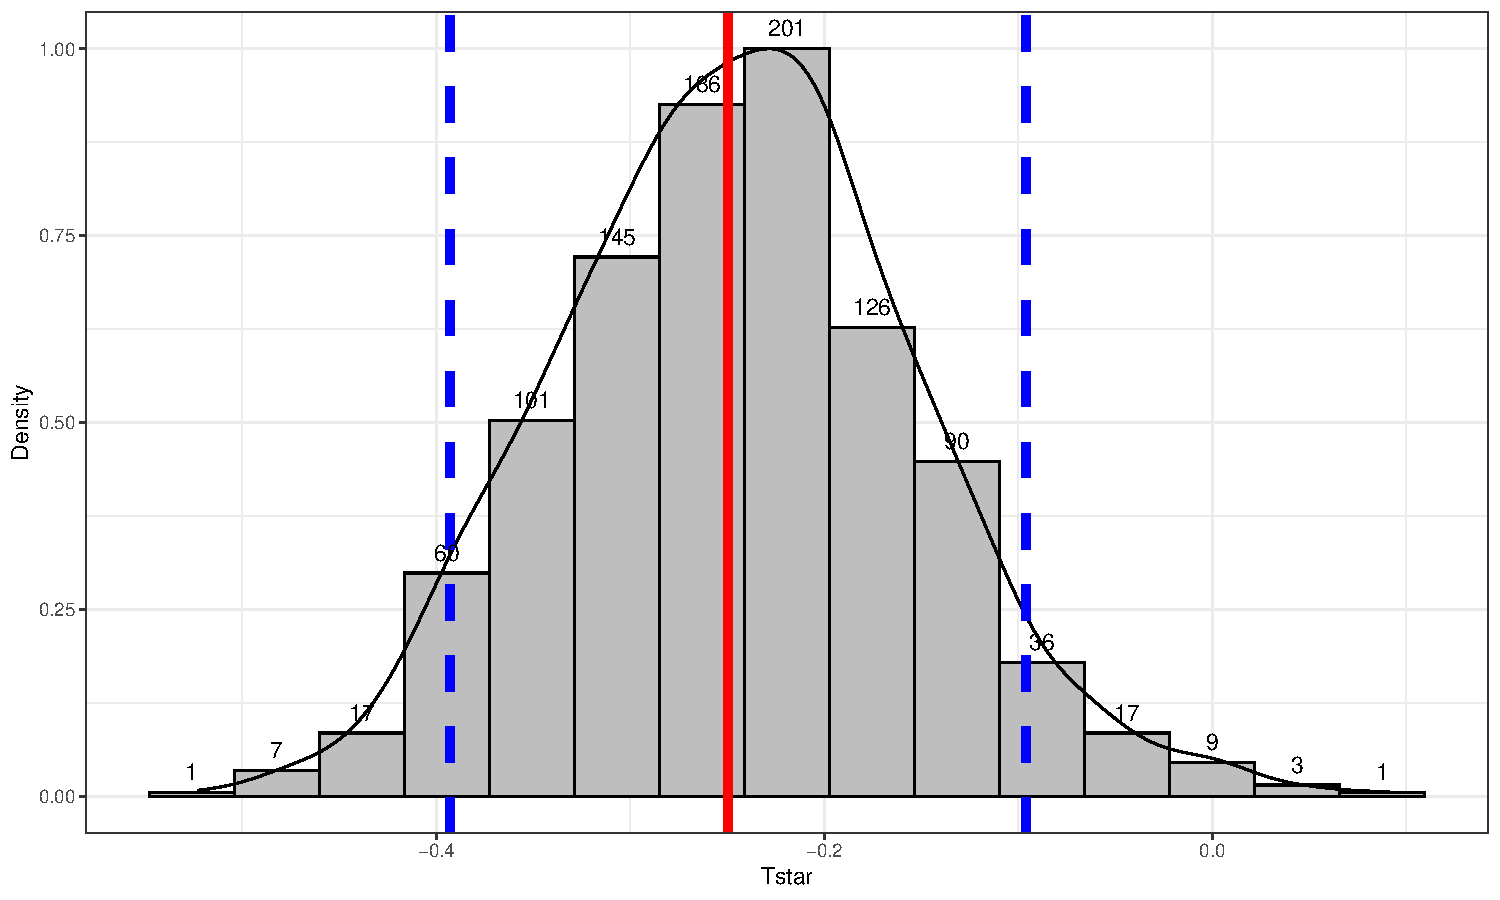
\includegraphics[width=0.75\linewidth]{02-linearmodelsreview_files/figure-latex/Figure2-26-1} 

}

\caption{Histogram and density curve of bootstrap distribution of difference in sample mean GPAs (male minus female) with observed difference (solid vertical line) and quantiles that delineate the 90\% confidence intervals (dashed vertical lines).}\label{fig:Figure2-26}
\end{figure}

\begin{Shaded}
\begin{Highlighting}[]
\FunctionTok{tibble}\NormalTok{(Tstar) }\SpecialCharTok{\%\textgreater{}\%} \FunctionTok{ggplot}\NormalTok{(}\FunctionTok{aes}\NormalTok{(}\AttributeTok{x =}\NormalTok{ Tstar)) }\SpecialCharTok{+} 
  \FunctionTok{geom\_histogram}\NormalTok{(}\FunctionTok{aes}\NormalTok{(}\AttributeTok{y =}\NormalTok{ ..ncount..), }\AttributeTok{bins =} \DecValTok{15}\NormalTok{, }\AttributeTok{col =} \DecValTok{1}\NormalTok{, }\AttributeTok{fill =} \StringTok{"grey"}\NormalTok{, }
                 \AttributeTok{center =} \DecValTok{0}\NormalTok{) }\SpecialCharTok{+} 
  \FunctionTok{geom\_density}\NormalTok{(}\FunctionTok{aes}\NormalTok{(}\AttributeTok{y =}\NormalTok{ ..scaled..)) }\SpecialCharTok{+}
  \FunctionTok{theme\_bw}\NormalTok{() }\SpecialCharTok{+}
  \FunctionTok{labs}\NormalTok{(}\AttributeTok{y =} \StringTok{"Density"}\NormalTok{) }\SpecialCharTok{+}
  \FunctionTok{geom\_vline}\NormalTok{(}\AttributeTok{xintercept =}\NormalTok{ quantiles, }\AttributeTok{col =} \StringTok{"blue"}\NormalTok{, }\AttributeTok{lwd =} \DecValTok{2}\NormalTok{, }\AttributeTok{lty =} \DecValTok{2}\NormalTok{) }\SpecialCharTok{+} 
  \FunctionTok{geom\_vline}\NormalTok{(}\AttributeTok{xintercept =}\NormalTok{ Tobs, }\AttributeTok{col =} \StringTok{"red"}\NormalTok{, }\AttributeTok{lwd =} \DecValTok{2}\NormalTok{) }\SpecialCharTok{+}
  \FunctionTok{stat\_bin}\NormalTok{(}\FunctionTok{aes}\NormalTok{(}\AttributeTok{y =}\NormalTok{ ..ncount.., }\AttributeTok{label =}\NormalTok{ ..count..), }\AttributeTok{bins =} \DecValTok{15}\NormalTok{, }
           \AttributeTok{geom =} \StringTok{"text"}\NormalTok{, }\AttributeTok{vjust =} \SpecialCharTok{{-}}\FloatTok{0.75}\NormalTok{)}
\end{Highlighting}
\end{Shaded}

In the previous output, the parametric 90\% confidence interval is from
-0.404 to -0.095, suggesting similar results again from the two approaches. Based on
the bootstrap CI, we can say that we are 90\% confident that the difference in
the true mean GPAs for STAT 217 students is between -0.393
to -0.096 GPA points
(male minus females). This result would be usefully added to step 5 in the 6+ steps of the hypothesis testing protocol with an updated result of:

\begin{enumerate}
\def\labelenumi{\arabic{enumi}.}
\setcounter{enumi}{4}
\item
  Report and discuss an estimate of the size of the differences, with confidence interval(s) if appropriate. \index{size interpretation}

  \begin{itemize}
  \tightlist
  \item
    Females were estimated to have a higher mean GPA by
    0.3 points (\emph{90\%
    bootstrap confidence interval: 0.096 to
    0.393}). This difference of
    0.3 on a GPA scale does not
    seem like a very large difference in the means even though we were able to
    detect a difference in the groups.
  \end{itemize}
\end{enumerate}

\indent Throughout the text, pay attention to the distinctions between parameters
and statistics, focusing on the differences between estimates based on the sample
and inferences for the population of interest in the form of the parameters of
interest. Remember that statistics are summaries of the sample information and
parameters are characteristics of populations (which we rarely know). And that
our inferences are limited to the population that we randomly sampled from, if
we randomly sampled.

\hypertarget{section2-11}{%
\section{Chapter summary}\label{section2-11}}

In this chapter, we reviewed basic statistical inference methods in the context
of a two-sample mean problem using linear models and the \texttt{lm} function. You were introduced to using R to do enhanced visualizations (pirate-plots), permutation
testing, and generate bootstrap confidence intervals as well as obtaining
parametric \(t\)-test and confidence intervals. You should
have learned how to use a \texttt{for} loop for doing the nonparametric inferences
and the \texttt{lm} and \texttt{confint} functions for generating parametric inferences. In the examples considered, the parametric and nonparametric methods provided similar
results, suggesting that the assumptions were not too violated for the parametric procedures. When parametric and nonparametric approaches
disagree, the nonparametric methods are likely to be more trustworthy since
they have less restrictive assumptions but can still make assumptions and can have problems.
\index{assumptions}

\indent When the noted conditions are violated in a hypothesis testing situation, the
Type I error \index{Type I error} rates can be inflated, meaning that we reject the null hypothesis
more often than we have allowed to occur by chance. Specifically, we could have
a situation where our assumed 5\% significance level test might actually reject
the null when it is true 20\% of the time. If this is occurring, we call a
procedure \textbf{\emph{liberal}} (it rejects too easily) and if the procedure is liberal,
how could we trust a small p-value to be a ``real'' result and not just an
artifact of violating the assumptions of the procedure? Likewise, for
confidence intervals we hope that our 95\% confidence level procedure, when
repeated, will contain the true parameter 95\% of the time. If our assumptions
are violated, we might actually have an 80\% confidence level procedure and it
makes it hard to trust the reported results for our observed data set.
Statistical inference relies on a belief in the methods underlying our
inferences. If we don't trust our assumptions, we shouldn't trust the
conclusions to perform the way we want them to. As sample sizes increase
and/or violations of conditions lessen, then the procedures will perform better.
In Chapter \ref{chapter3}, some new tools for doing diagnostics are introduced
to help us assess how and how much those validity conditions are violated.

\indent It is good to review how to report hypothesis test conclusions and compare those for when we have strong, moderate, or weak evidence. Suppose that we are doing parametric inferences with \texttt{lm} for differences between groups A and B, are extracting the \(t\)-statistics, have 15 degrees of freedom, and obtain the following test statistics and p-values:

\begin{itemize}
\item
  \(t_{15} = 3.5\), p-value = 0.0016:

  There is strong evidence against the null hypothesis of no difference in the true means of the response between A and B (\(t_{15} = 3.5\), p-value = 0.0016), so we would conclude that there is a difference in the true means.
\end{itemize}

\begin{itemize}
\item
  \(t_{15} = 1.75\), p-value = 0.0503:

  There is moderate evidence against the null hypothesis of no difference in the true means of the response between A and B (\(t_{15} = 1.75\), p-value = 0.0503), so we would conclude that there is likely\footnote{Note that this modifier is added to note less certainty than when we encounter strong evidence against the null. Also note that someone else might decide that this more like weak evidence against the null and might choose to interpret it as in the ``weak'' case. In cases that are near boundaries for evidence levels, it becomes difficult to find a universal answer and it is best to report that the evidence is both not strong and not weak and is somewhere in between and let the reader decide what they think it means to them. This is complicated by often needing to make decisions about next steps based on p-values where we might choose to focus on the model with a difference or without it.} a difference in the true means.
\item
  \(t_{15} = 0.75\), p-value = 0.232:

  There is weak evidence against the null hypothesis of no difference in the true means of the response between A and B (\(t_{15} = 0.75\), p-value = 0.232), so we would conclude that there is likely not a difference in the true means.
\end{itemize}

The last conclusion also suggests an action to take when we encounter weak evidence against null hypotheses -- we could potentially model the responses using the null model since we couldn't prove it was wrong. We would take this action knowing that we could be wrong, but the ``simpler'' model that the null hypothesis suggests is often an attractive option in very complex models, such as what we are going to encounter in the coming chapters, especially in Chapters \ref{chapter5} and \ref{chapter8}.

\hypertarget{section2-12}{%
\section{Summary of important R code}\label{section2-12}}

The main components of R code used in this chapter follow with components to
modify in lighter and/or ALL CAPS text, remembering that any R packages mentioned
need to be installed and loaded for this code to have a chance of working:

\begin{itemize}
\item
  \textbf{summary(\textcolor{red}{DATASETNAME})}

  \begin{itemize}
  \tightlist
  \item
    Provides numerical summaries of all variables in the data set.
    \index{\texttt{summary()}|textbf}
  \end{itemize}
\item
  \textbf{summary(lm(\textcolor{red}{Y} \textasciitilde{} \textcolor{red}{X},
  data = \textcolor{red}{DATASETNAME}))}

  \begin{itemize}
  \tightlist
  \item
    Provides estimate, SE, test statistic, and p-value for difference in second row of coefficient table. \index{\texttt{summary(lm())}|textbf}
  \end{itemize}
\item
  \textbf{confint(lm(\textcolor{red}{Y} \textasciitilde{} \textcolor{red}{X},
  data = \textcolor{red}{DATASETNAME}), level = 0.95)}

  \begin{itemize}
  \tightlist
  \item
    Provides 95\%
    confidence interval for difference in second row of output. \index{\texttt{confint(lm())}|textbf}
  \end{itemize}
\item
  \textbf{2\texttt{*}pt(abs(\textcolor{red}{Tobs}), df = \textcolor{red}{DF}, lower.tail = F)}

  \begin{itemize}
  \tightlist
  \item
    Finds the two-sided test p-value for an observed 2-sample t-test
    statistic of \texttt{Tobs}. \index{\texttt{pt()}|textbf}
  \end{itemize}
\item
  \textbf{hist(\textcolor{red}{DATASETNAME\$Y})}

  \begin{itemize}
  \tightlist
  \item
    Makes a histogram of a variable named \texttt{Y} from the data set of
    interest.
  \end{itemize}
\item
  \textbf{boxplot(\textcolor{red}{Y} \textasciitilde{} \textcolor{red}{X}, data = \textcolor{red}{DATASETNAME})}

  \begin{itemize}
  \tightlist
  \item
    Makes a boxplot of a variable named Y for groups in X from the data set.
  \end{itemize}
\item
  \textbf{pirateplot(\textcolor{red}{Y} \textasciitilde{} \textcolor{red}{X}, data = \textcolor{red}{DATASETNAME}, inf.method = ``ci'', inf.disp = ``line'')}

  \begin{itemize}
  \item
    Requires the \texttt{yarrr} package is loaded.
  \item
    Makes a pirate-plot of a variable named Y for groups in X from the data set with estimated means and 95\% confidence intervals for each group. \index{\texttt{pirateplot()}|textbf}
  \item
    Add \texttt{theme\ =\ 2} if the confidence intervals extend outside the density curves and you can't see how far they extend.
  \end{itemize}
\item
  \textbf{mean(\textcolor{red}{Y} \textasciitilde{} \textcolor{red}{X}, data = \textcolor{red}{DATASETNAME}); sd(\textcolor{red}{Y} \textasciitilde{} \textcolor{red}{X}, data = \textcolor{red}{DATASETNAME})}

  \begin{itemize}
  \item
    This usage of \texttt{mean} and \texttt{sd} requires the \texttt{mosaic} package.
  \item
    Provides the mean and sd of responses of Y for each group described in X.
  \end{itemize}
\item
  \textbf{favstats(\textcolor{red}{Y} \textasciitilde{} \textcolor{red}{X}, data = \textcolor{red}{DATASETNAME})}

  \begin{itemize}
  \tightlist
  \item
    Provides numerical summaries of Y by groups described in X.
  \end{itemize}
\item
  \textbf{Tobs \texttt{\textless{}-} coef(lm(\textcolor{red}{Y} \textasciitilde{} \textcolor{red}{X}, data = \textcolor{red}{DATASETNAME})){[}2{]}; Tobs\\
  B \texttt{\textless{}-} 1000\\
  Tstar \texttt{\textless{}-} matrix(NA, nrow = B)\\
  for (b in (1:B))\{\\
  lmP \texttt{\textless{}-} lm(\textcolor{red}{Y} \textasciitilde{} shuffle(\textcolor{red}{X}), data = \textcolor{red}{DATASETNAME})\\
  Tstar{[}b{]} \texttt{\textless{}-} coef(lmP){[}2{]}\\
  \}}

  \begin{itemize}
  \tightlist
  \item
    Code to run a \texttt{for} loop to generate 1000 permuted versions of the test
    statistic using the \texttt{shuffle} function and keep track of the results in
    \texttt{Tstar}
  \end{itemize}
\item
  \textbf{pdata(Tstar, abs(\textcolor{red}{Tobs}), lower.tail = F){[}{[}1{]}{]}}

  \begin{itemize}
  \tightlist
  \item
    Finds the proportion of the permuted test statistics in Tstar that are
    less than -\textbar Tobs\textbar{} or greater than \textbar Tobs\textbar, useful for finding the two-sided
    test p-value. \index{\texttt{pdata()}|textbf}
  \end{itemize}
\end{itemize}

\begin{itemize}
\item
  \textbf{Tobs \texttt{\textless{}-} coef(lm(\textcolor{red}{Y} \textasciitilde{} \textcolor{red}{X}, data = \textcolor{red}{DATASETNAME})){[}2{]}; Tobs\\
  B \texttt{\textless{}-} 1000\\
  Tstar \texttt{\textless{}-} matrix(NA, nrow = B)\\
  for (b in (1:B))\{\\
  lmP \texttt{\textless{}-} lm(\textcolor{red}{Y} \textasciitilde{} \textcolor{red}{X}, data = resample(\textcolor{red}{DATASETNAME}))\\
  Tstar{[}b{]} \texttt{\textless{}-} coef(lmP){[}2{]}\\
  \}}

  \begin{itemize}
  \tightlist
  \item
    Code to run a \texttt{for} loop to generate 1000 bootstrapped versions of the
    data set using the \texttt{resample} function and keep track of the results of
    the statistic in \texttt{Tstar}.
  \end{itemize}
\end{itemize}

\newpage

\begin{itemize}
\item
  \textbf{qdata(Tstar, c(0.025, 0.975))}

  \begin{itemize}
  \tightlist
  \item
    Provides the values that delineate the middle 95\% of the results in the
    bootstrap distribution (\texttt{Tstar}). \index{\texttt{qdata()}|textbf}
  \end{itemize}
\end{itemize}

\hypertarget{section2-13}{%
\section{Practice problems}\label{section2-13}}

2.1. \textbf{Overtake Distance Analysis} The tests for the overtake distance data were performed with two-sided alternatives and so two-sided areas used to find the p-values. Suppose that the researchers expected that the average passing distance would be less (closer) for the commute clothing than for the casual clothing group. Repeat obtaining the permutation-based p-value for the one-sided test for either the full or smaller sample data set. Hint: Your p-value should be just about half of what it was before and in the direction of the alternative.

\vspace{11pt}

2.2. \textbf{HELP Study Data Analysis} Load the \texttt{HELPrct} data set from the \texttt{mosaicData} package (\protect\hyperlink{ref-R-mosaicData}{Pruim, Kaplan, and Horton 2021b})
(you need to
install the \texttt{mosaicData} package once to be able to load it). The HELP study
was a clinical trial for adult inpatients recruited from a
detoxification unit. Patients with no primary care physician were randomly
assigned to receive a multidisciplinary assessment and a brief motivational
intervention or usual care and various outcomes were observed. Two of the
variables in the data set are \texttt{sex}, a factor with levels \emph{male} and \emph{female}
and \texttt{daysanysub} which is the time (in days) to first use of any substance
post-detox. We are interested in the difference in mean number of days to first
use of any substance post-detox between males and females. There are some
missing responses and the following code will produce \texttt{favstats} with the
missing values and then provide a data set that by
applying the \texttt{drop\_na()} function to the piped data set removes any observations with missing values. \index{\texttt{drop\_na()}} \index{R packages!\textbf{mosaicData}}

\begin{Shaded}
\begin{Highlighting}[]
\FunctionTok{library}\NormalTok{(mosaicData)}
\FunctionTok{data}\NormalTok{(HELPrct)}
\CommentTok{\# Just focus on two variables}
\NormalTok{HELPrct2 }\OtherTok{\textless{}{-}}\NormalTok{ HELPrct }\SpecialCharTok{\%\textgreater{}\%} \FunctionTok{select}\NormalTok{(daysanysub, sex) }
\CommentTok{\# Removes subjects (complete rows) with any missing values}
\NormalTok{HELPrct3 }\OtherTok{\textless{}{-}}\NormalTok{ HELPrct2 }\SpecialCharTok{\%\textgreater{}\%} \FunctionTok{drop\_na}\NormalTok{() }
\FunctionTok{favstats}\NormalTok{(daysanysub }\SpecialCharTok{\textasciitilde{}}\NormalTok{ sex, }\AttributeTok{data =}\NormalTok{ HELPrct2)}
\FunctionTok{favstats}\NormalTok{(daysanysub }\SpecialCharTok{\textasciitilde{}}\NormalTok{ sex, }\AttributeTok{data =}\NormalTok{ HELPrct3)}
\end{Highlighting}
\end{Shaded}

2.2.1. Based on the results provided, how many observations were missing for males
and females? Missing values here likely mean that the subjects didn't use any
substances post-detox in the time of the study but might have at a later
date -- the study just didn't run long enough. This is called \textbf{\emph{censoring}}.
What is the problem with the numerical summaries here if the missing responses
were all something larger than the largest observation?

2.2.2. Make a pirate-plot and a boxplot of \texttt{daysanysub} \textasciitilde{} \texttt{sex} using the
\texttt{HELPrct3} data set created above. Compare the distributions, recommending
parametric or nonparametric inferences.

2.2.3. Generate the permutation results and write out the 6+ steps of the
hypothesis test.

2.2.4. Interpret the p-value for these results.

2.2.5. Generate the parametric test results using \texttt{lm}, reporting the test-statistic,
its distribution under the null hypothesis, and compare the p-value to those
observed using the permutation approach.

2.2.6. Make and interpret a 95\% bootstrap confidence interval for the difference
in the means.

\hypertarget{chapter3}{%
\chapter{Identifying the Model: Study designs/sampling methods}\label{chapter3}}

While the technical details of estimating and doing inference are like a ball of yarn to a kitten and can usefully distract you for years of exploring this material, this chapter discusses how data are generated and provides tools for thinking designing your own studies. I more often work with data from studies that have either been designed and the data were already collected (prior to consultation with a statistician) or in observational studies, where ``design'' is not chosen by the researchers but by the process (although the choice to collect and analyze it in any particular form is, in some sense, a ``design''). There are many resources that can help to implement complex randomization schemes and take you through designing your own experiments - that is not my goal here. We will focus on asking hard questions of the study and data collection process to elicit the correct model structure. While doing this, you might actually learn some principles of designing experiments, but the goal here is more on finding the right model, given a design, rather than on designing the best experiment in a given situation.

As part of this chapter, I will also introduce a number of different data sets we will revisit later in the semester and some diagramming tools that will be a prominent component of our modeling process as well as the model summarizations.

\hypertarget{section3-1}{%
\section{``Measurement'' structure}\label{section3-1}}

\indent The simplest data set to analyze is a \textbf{cross-sectional} data set with no inherent groups. This is the scenario that leads to assuming that all observations are independent of one another. This study design fits clearly with using \texttt{lm} to analyze data with models such as One-Way ANOVA, Two-Way ANOVA, simple and multiple linear regression, and such simple procedures at the two-independent sample t-test (which is just a two-group Two-Way ANOVA, if no one told you that yet). Independence of observations is also an inherent assumption in basic nonparametric and simple randomization procedures. While this design and these analyses cover the majority of statistical methods used in practice, when you actually dig into many study designs there are additional complexities lurking and often unaccounted for.

\indent You can think of violations of the independence assumption as any source of systematically similar or dissimilar groups of rows of observations in the data set. The most clear of the violations is taking repeated measures on the same subject but other related examples would be taking measurements of a group of students in the same classroom or from patients that are getting treatment in different hospitals or plants that are grouped together in plots within a field. In all of these cases, we might think that ``neighbors'' (multiple observations on the same subject or from the same class or in the same plot) might be more similar on some response we measure within a group and less similar to those outside the group. These are all examples of \textbf{two-level} situations where our main task initially is to account for subject-to-subject, class-to-class, or hospital-to-hospital variability. In Chapter 7 (link), we will explore the \textbf{random intercept} models as a starting point for doing this. There are always extensions, but for two-level situations, the focus is on accounting for systematic differences at the higher level which allows for random variability that is independent across observations at the **observation'' level (conditional on the random subject or group variability, the remaining errors are independent).

Two-level situations go by a variety of different ``names'', some hinting at how the data are collected. For example, repeated measures (usually over time) on the same subjects are called (not surprisingly) repeated measures data or are called longitudinal data or ?\ldots{} When there are experimental units that are physically split apart to create experimental units, such as when fields are split into rows and one observation is made per row, this is called a \textbf{split-plot} design. {[}Other name from education?{]} In all of these designs, we can start with the same random-intercept model. So to me, the ``name'' of the design is less important than what the level of grouping is called and what I need to do to account for it in a model.

\indent And it is possible for these similar/dissimilar measurements to come in layers or a hierarchy, where there are groups of ``neighbors'' within larger groups of ``neighbors. Extending each of the previous examples, the repeated measures on the same subject could come from groups of students in the same classes or patients in the same hospitals or plants in the same fields. Theses create multi-level (here meaning more than two levels) hierarchies that we need to account. These come with specific names of designs partially discussed below, but I generally try to think about the hierarchies and how to account for them, rather than the specific name of the design that lead to the data that were collected. I find this more general approach to help me to handle additional complexities that do not fit into a''named'' design and to test my ideas of what the actual design might be. In these cases (Chapter 8 (link)), we start with random intercepts for each level of the hierarchy (except for the observation level) in order to account for systematic variability at each level. The top\footnote{More on numbering levels in a bit, as that has two ways to do it} level is accounted for in a way that is similar to the two-level model with a random intercept. For the grouping within the top level groups, \ldots. nesting\ldots{} so \textbf{nested} random intercepts are incorporated. Just as in the two-level model, there is an assumption of random variation that is independent at the observation level once we account for the systematic variation at higher levels of the model.

Like for two-level models, the same multi-level model can account for data collection schemes that go by different names (or are often un-named). Specifically, a \textbf{split-split plot} desing is a three-level design where there observational units that are split up physically in a hierarchical way twice (say fields that are split into rows of the field and then the rows are split to get multiple observations within a row). But a ``split-plot'' design where repeated measures are taken on each row in the field would also result in a three-level situation (fields, rows in fields, and observations on the rows in the fields over time). I would not call the second situation a ``split-split plot'' but the model for it and the one with rows sub-divided would be analyzed with essentially the same statistical model to handle the hierarchies.

Three-level models seem complex, but for reasons I sometimes struggle to understand, researchers often endeavor to work with more complex situations\footnote{Or graduate students are ``encouraged'' by their advisors to do this, which seems more common for the source of this.}. Sometimes this is because of the way measurements must be taken and sometimes it is just an overcomplication. You can read a great and very humble discussion of this in {[}{]}, where {[}{]} discusses a project he did. He \ldots. and found that the results would be very similar if he had just averaged to the pond level instead of trying to analyze the results at the {[}{]} level. That said, there are some reasons to avoid aggregation. My most common are (1) differing sample size or variance at the lowest level of the hierarchy, (2) explanatory variables that vary at the lowest level of the hierarachy and (in their measured form) can explain variation at the level of observations, and/or (3) there are potentially problematic (think outlier or contaminated measurements) at the observation level and aggregating would remove the chance to identify and investigate those unusual points before combining them with others.

Sample size

Random assigned, level of variation of fixed effects

Diagrams

\indent In the following, I am drawing on twenty years of experience and a good number of mistakes and ``wandering'' in trying to arrive at the correct model for a given data set. This is one of the most complex aspects of doing mixed models as there are often multiple options for how to think about the ``groups'' and this leads to multiple models that could be fit and often quite different results from the models.

{[}move{]} All of these methods have extensions to non-independent data and I will spend the rest of this book going through how we can use mixed models to account for various violations of the independence of observations assumptions.

\begin{itemize}
\tightlist
\item
  General questions to ask to determine the study design
\end{itemize}

\hypertarget{section3-2}{%
\section{``Measurement'' diagrams}\label{section3-2}}

This

\hypertarget{section3-3}{%
\section{Effective sample size and degrees of freedom}\label{section3-3}}

This

\hypertarget{section3-4}{%
\section{Visualizing observed predictors}\label{section3-4}}

alluvial

tableplot

ggpairs

heatmap of predictors/ sorting predictor variables

corrplot.mg

\hypertarget{section3-5}{%
\section{Multiple (pair-wise) comparisons using Tukey's HSD and the compact letter display}\label{section3-5}}

\indent There is a method that many researchers use to more efficiently generate and
report these sorts of results that is called a \textbf{\emph{compact letter display}} \index{compact letter display}
(CLD, Piepho (\protect\hyperlink{ref-Piepho2004}{2004}))\footnote{Note that this method is implemented slightly differently than explained here in some software packages so if you see this in a journal article, read the discussion carefully.}. The \texttt{cld} function can be applied to the results from

\hypertarget{chapter4}{%
\chapter{Identifying the Model: Response}\label{chapter4}}

{[}image here{]}

\hypertarget{section4-1}{%
\section{Situation}\label{section4-1}}

For any of the designs and measurement structures from Chapter \ref{chapter3}, there is a variety of ways to measure our potential response variable. This usually starts with responses that can be modeled with linear models that are assumed to be continuous, quantitative, and not bounded - and that hopefully end up with models with residuals that are normally distributed (our normality assumption). These models have a normality assumption on the response (\(Y \sim N(\mu, \sigma^2)\)) that drives our inferences as well as relates to some of the diagnostics we used. As discussed in Chapter \ref{chapter1}, we can sometimes find a suitable transformation of the response to then allow linear models to be used and have residuals that follow normal distributions, or sometimes we can incorporate random effects, non-constant variance and/or correlation structures and that can improve the normality of the residuals and keep us within the regular normality of residuals situation.

But not all responses fit with the normality assumption or can be transformed and modeled to have residuals that are normal - even some quantitative responses have issues that involve boundaries or censoring that complicate modeling. For example, sometimes measurements are a proportion of a total, such as the proportion of a total sample of liquid that is a particular compound or the proportion of a day where an animal engaged in some activity or the proportion of a square that is covered by a particular type of plant. We know that this can't be less than 0 or over 1. The measurements can be continuous (or are sometimes discrete) but bounded, so the residuals often do not follow a normal distribution. {[}cite/discuss Irvine paper{]} These responses can be transformed using the arcsine-square-root {[}cite{]} or natural log or log-odds to alleviate the boundaries (but only if the responses never attain either boundary for the arcsince-square-root or 0 for the log-based transformations - although some use an adjustment at the edges to avoid hitting 0 or 1. The main point of this discussion is to be aware that some continuous responses may not be suitable for use in a linear model, although if most of the responses are far from these boundaries, sometimes the residuals will be reasonably close to normality for a linear model to be reasonably applied or applied after one of the transformations mentioned.

To add to the discussion of boundaries in quantitative measurements, sometimes there are detection limits in the measurement process and only trustworthy measurements are available when the true amount is over some lower limit and/or above some upper limit of detection, creating \textbf{censoring} of the measurements when in these areas of lower quality or completely unobservable measurements. In one example, if counts of cases of a certain type in a country were below five, the reporting agency would censor them and report that the count was lower than five\footnote{In one case, they would report 0 cases as 0, so only 1 to 4 were actually censored, but since I don't have a good way to handle this situation, I went with the simpler situation of censoring below a value.}. In metabolomics research (for example, cite Hahn \ldots), it is common to observations censored as a lower detection limit where the machine is not able to differentiate signal from noise\footnote{This is found by running ``blanks'' through the machine and looking at signal strength for a metabolite when ``none'' is present - this is then the limit of detection for a ``real'' signal and anything below that value is typically set to 0, coded as missing, or filled in with some number between the lower detection limit and 0}. In water monitoring, streamflow height is often measured, but if the river gets very low or very high, the observation for a given time can go outside the detection limits of the streamflow gauge, creating censoring for both low and high values. I will discuss some references to explore for modeling these situations, but the point here is to present potential issues with continuous (or at least quantitative measurements) that should be probed before blindly using linear models.

A related source of a quantitative measurement with a lower bound and sometimes censored responses is when the time to event occurring is measured, but this requires a different sort of modeling approach that is beyond the scope of this book, called survival or duration analysis. These measurements have a lower bound of 0 (no time to event occuring) and an upper bound of \(\infty\) (the event could never occur). When you look for information on censored responses, survival analysis will populate your search as these data are prone to unobserved outcomes where a subject is observed for some period of time and no event occurs (so the actual time of the event is unknown but is longer than the time of observation of that subject). This is mentioned so you are aware of these type of quantitative measurements to avoid trying to fit them into the models we will discuss here. The Cox proportional hazards model that is often used with survival data will be more understandable after reading the logistic regression discussion here, but I will not attempt to develop it further. You can read more about survival analysis in {[}cite{]}.

Other issues with normality of residuals stem from clear violations of normality of responses, where by their very nature, observations are not nor should they be modeled as normal. The most common of these is a binary response, where an observation can be considered a ``success'' or ``failure''. I put these in quotes because (1) it is your\footnote{R will make a choice for you but that can be modified, as we will discuss later.} choice which is defined as a success or failure and (2) sometimes a ``success'' will be the outcome that has a negative connotation, such as getting cancer or dying from a disease. With just two options, even if coded as 0s and 1s, the response and any linear models residuals for it would never be normally distributed. This fits into treating the response as Bernoulli or Binomial distributed (Binomial with just one observation, not ``grouped''), matching the response with a ``named'' distribution other than normal to more appropriately model the response pattern.

Another type of response is to count the number of a type of thing in an area or volume. This has a domain of measurements of 0, 1, 2, \(\dots\), \(\infty\), with the discreteness making modeling assuming linearity problematic. We can more appropriately model counts like these starting with \textbf{Poisson} models. I say ``starting with'' because we will also use a Negative Binomial distribution for modeling these responses and discuss modifications for when there are no or too many zeros (relative to what the Poisson expects), but the underlying process starts with Poisson. It is a model that follows with the definition of counting something, where you can only observe 0 or 1 or 2 or \ldots{} of a thing. When counts get very large (means over 100 and rarely below 10\footnote{}), then log-transforming the counts can provide models with approximately normal residuals from linear models. \textbf{Poisson rate} models extend the basic count model to directly incorporate the effort (area, volume, time, etc.) spent in collecting each observation. Some researchers will pre-divide the counts by these efforts to create a ``count per \ldots{}'' observation and try to model this with linear models or log-transform and then model as a linear model. We will get different and better results by treating the Poisson rate responses directly as a count process with information included in the model about the efforts (see XXX for an example of this).

There is another type of count to be aware of that extends the Bernoulli response discussion and incorporates an upper bound into the counting, when we count the number of successes out of some total number of things examined. Think about looking at a plant and examining 20 leaves of the plant for insect damage and possibly finding 5 that had damage and 15 that were not damaged. These are counts, but counts with an upper limit for the total number that can be seen. This is an extension of the Bernoulli situation and uses more or less the same model, as discussed later, but is called the \textbf{grouped Binomial}.

Another consideration in determining which modeling framework to consider is univariate or multivariate responses. A multivariate response is when there is more than one outcome variable measured per subject. Sometimes this is related to repeated measures on the same variable (discussed in full detail in Chapter ?). But another type of multivariate response is when a variety of different measurements are taken on the same sample or subject. In plant sciences, for example, the plants are often weighed and the amount of certain minerals are measured (like Nitrogen) and the roots are also weighed and\ldots{} Or in the metabolomics area, a suite of hundreds or thousands of different compounts can be quantified. And in survey research, researchers often ask participants to answer dozens or even hundreds of questions, with each being a potential response variable of interest. We have four choices: (1) model each response separately, (2) use a multivariate response model that directly works with the multiple responses and models the correlation among them, (3) use a dimension reduction technique - most often factor analysis or the related aggregation using a total or mean across a suite of items to create a single\footnote{Sometimes this leads to more than one variable but much less than the original number.} variable to analyze, and (4) use one or more outcomes to explain another outcome, possibly with an interaction (often called analysis of covariance (ANCOVA) models). Of these, (1) is the simplest and just takes brute force to analyze all the response, but creates some need to consider multiple testing adjustments to avoid inflated Type I error rates as you search across so many outcomes (see \url{https://greenwood-stat.github.io/GreenwoodBookHTML/chapter2.html\#section2-8} for more on this). (2) can be useful to leverage correlation among responses but can be difficult to interpret and so often is followed up with (1) to really understand results (certainly in the Multivariate ANOVA or MANOVA models, possibly in other cases). (3) is commonly done without too much discussion as a way of avoiding doing either (1) or (2), but still sometimes results in more than one response. In general, there are many ``variables'' that I encounter that are derived from the raw original measurements using a mean, median, total, or other combining function. This combining often eliminates level(s) in a hierarchy as discussed in Chapter \ref{chapter3} and so can also simplify the modeling process. But remember that any combining can also lose information on the precision (and differences among precision) those values. (4) really changes the research question to studying relationships among responses, with one chosen as a more interesting target, possibly modifying that relationship based on levels of another variable, like a treatment was applied to the subject. Here, the focus will be on (1), but connections and extensions to these other situations will also be noted where possible. Often when pressed a researcher can identify a primary outcome of interest, with secondary outcomes that are also of interest but of lesser importance. This makes the focus on (1) a reasonable starting point for this book.

Figure \ref{fig:Figure4-1} tries to lay out a diagram as a starting point for this discussion with endpoints for starting points for software to use to fit initial models for the scenarios considered here. I say initial models because modeling is an iterative process and model assumptions must be probed and questioned to trust what the models are telling us. While we have seen some diagnostics for linear models and many extend to the new methods discussed here, it is helpful to explore some data visualization techniques that are specific to each type of response and learn how to use and interpret them. They are not necessarily diagnostics, but can help to explain your data and your modeling choices and sometimes suggest new directions for research.

Flow chart of methods. Flow chart of response types and possible models.

\begin{figure}[ht!]

{\centering 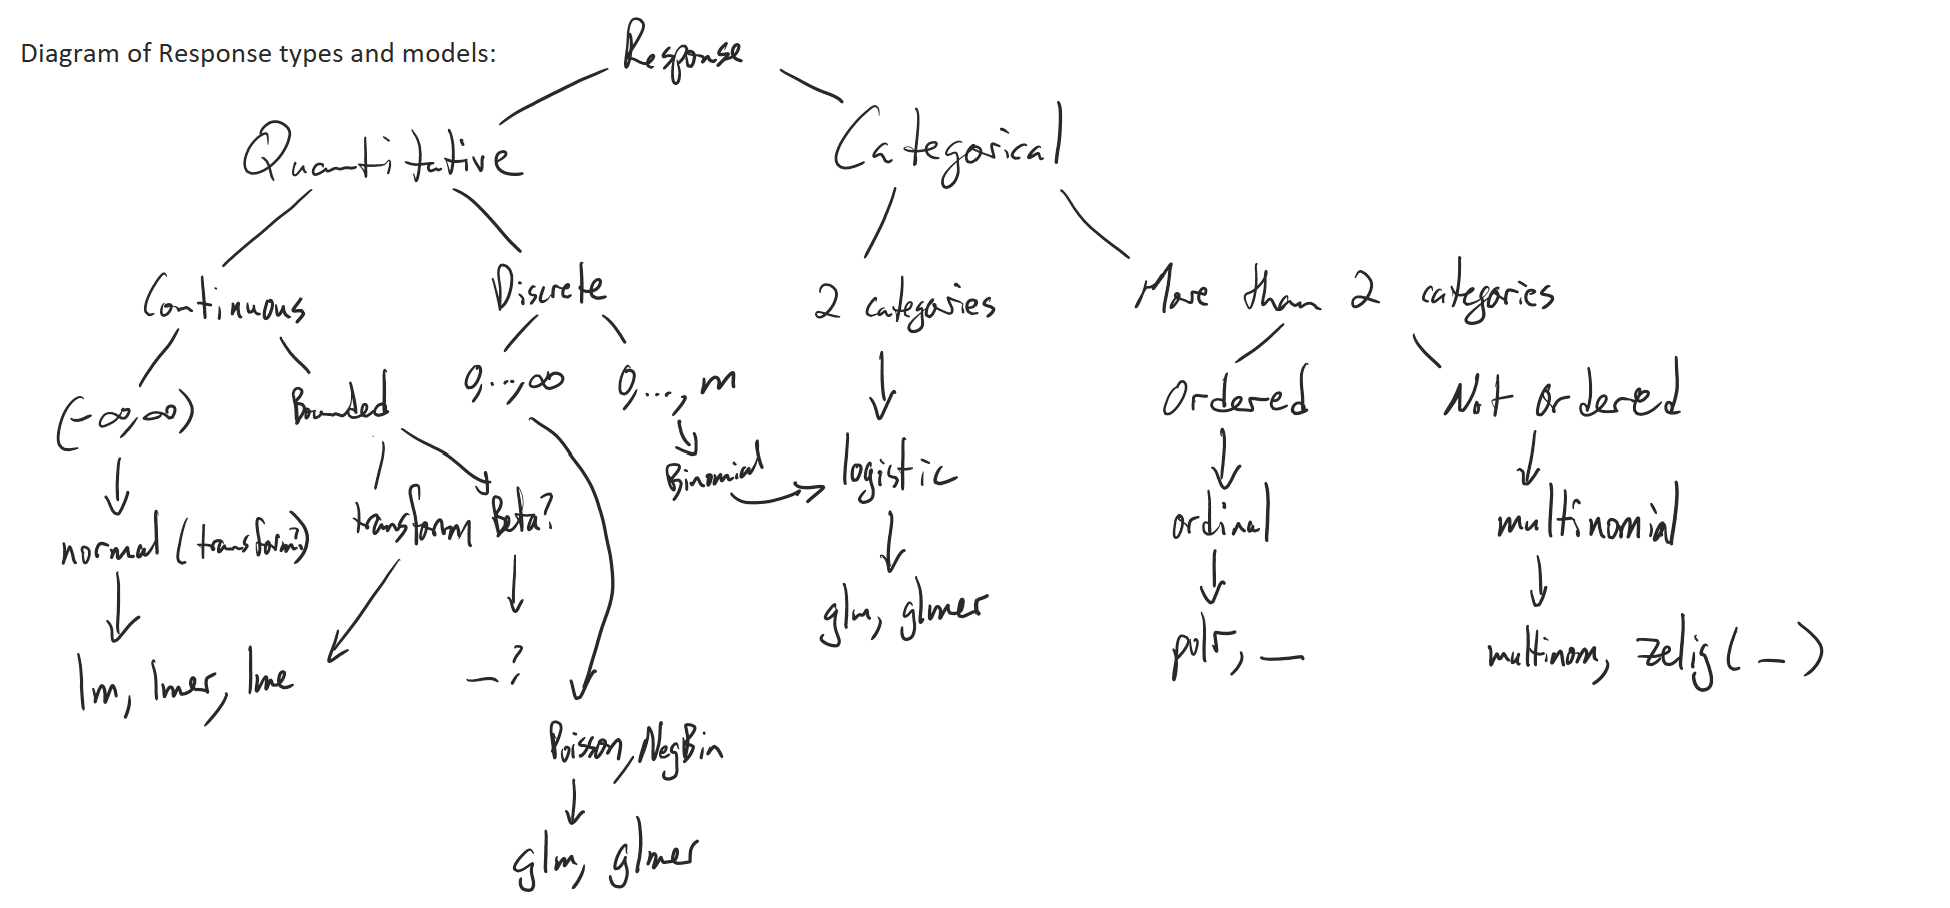
\includegraphics[width=0.75\linewidth]{responsediagram} 

}

\caption{(ref:fig4-1)}\label{fig:Figure4-1}
\end{figure}

\hypertarget{section4-2}{%
\section{The generalized linear model}\label{section4-2}}

In the previous diagram, there are discussions of responses that follow distributions other than normal. To frame how to handle these responses, the \textbf{generalized linear} model framework is needed. Each of these models and interpretations is discussed in detail in Chapter @ref\{Chapter11\}, but this section helps to put names and model structures together in one place. There are three components to a

{[}grab X12 notes to start this discussion{]}

\hypertarget{section4-3}{%
\section{Multiple (pair-wise) comparisons using Tukey's HSD and the compact letter display}\label{section4-3}}

\indent There is a method that many researchers use to more efficiently generate and
report these sorts of results that is called a \textbf{\emph{compact letter display}} \index{compact letter display}
(CLD, Piepho (\protect\hyperlink{ref-Piepho2004}{2004}))\footnote{Note that this method is implemented slightly differently than explained here in some software packages so if you see this in a journal article, read the discussion carefully.}. The \texttt{cld} function can be applied to the results from

\hypertarget{chapter5}{%
\chapter{Data visualization and data wrangling for hierarchical data}\label{chapter5}}

\hypertarget{section5-1}{%
\section{Situation}\label{section5-1}}

In Chapter \ref{chapter4}, a suite of different models and types of responses are defined, along with some potential models for those responses. Here, some specific data visualization tools and data wrangling techniques are discussed.

Data visualization provides ways to ask questions of our data that relate to model choice and develop expectations for results from models, to understand likely complications or limitations in the modeling process, and even to suggest new models. I do not suggest ``mining'' your data for research questions - these should be developed \emph{a priori}, but if your research question is about the relationship between two variables, the RQ might need to change if that relationship seems to be different across levels of another variable (like in ANCOVA settings). Data visualization can also help to suggest model modifications for the response (transformations or changing the proposed response distribution as in zero-inflated or zero-truncated counts) and systematic components (transformations or polynomials or splines for curving relationships) or to target certain unusual observations for further investigation prior to fitting a model (remember the Chapter \ref{Chapter1} discussion about non-influential outliers that can impact the distribution of residuals and influential observations that can impact and distort the fit of the models).

In order to facilitate our modeling and data visualization, there are three possibly new data wrangling skills that are needed. There are related tasks that are needed with hierarchical and especially repeated measures data. In ``simple''\footnote{These really are not simple and often this is used in more complex designs too.} two-level designs where repeated measures are taken on a subject, the observations are often organized in a wide fashion, with one row per subject and repeated time points on the same variable placed in different columns. This is great for data entry simplicity but often not compatible with our models (all the responses need to be in a single column with an additional column indicating which time point they came from). Also to utilize the full power of ggplot2 {[}cite{]} for data visualization, we need the same sort of ``responses in a column'' format. The `pivot\_longer' function and its related `pivot\_wider' functions from \texttt{dplyr} {[}cite{]} provide ways of pivoting into the ``long format'' data that we need and then back to ``wide format''. Sometimes data are collected in two or more different locations, the wide format longitudinal data, for example, and a second spreadsheet of demographics for each subject that are not changing over time (\textbf{static}). The `left\_join' function from `dplyr' provides a way to link the long format longitudinal information to repeatedly looking up and copying the static demographic data based on a linking subject identifier in both spreadsheets (think ``subject ID''). Finally, sometimes there is a need to take information and aggregate it to a higher level of the measurement hierarchy to create a new version of a predictor variable, which can be done with \texttt{ave} function when means are needed or more generally using `dplyr' and its `group\_by' function. Section {[}5-2{]} explores each of the functions and demonstrates them with two examples.

\hypertarget{section5-2}{%
\section{Data wrangling for longitudinal data}\label{section5-2}}

\begin{itemize}
\item
  Student test data - maybe find another example from base R?
\item
  Simulated IQ and beers example?
\end{itemize}

\hypertarget{section5-3}{%
\section{Data visualizations and summaries for missing data}\label{section5-3}}

Missing data are a reality of many real studies, sometimes systematically and sometimes by accident (also known as demonic intrusion). One can think of the missingness often as being driven by a random process, but that random process could be related to \ldots{}

\hypertarget{section5-4}{%
\section{Data vizualizations for non-normal responses}\label{section5-4}}

For non-normal responses (binary, multi-category, and counts), there are some specific plots that allow exploration of the responses that extend beyond scatterplots and boxplots. Specifically, conditional density plots (`cdplot' or `geom\_density' from `ggplot2') allow visualization of categorical response versus a quantitative predictor, displaying estimated probabilities of each category across the range of the observed predictor variable. The base R `plot' function provides a `spineplot' when used to explore a categorical response versus a categorical predictor - although we can find a similar plot using {[}????{]} from `ggplot2'. There is also the `mosaicplot' that is discussed in detail in \url{https://greenwood-stat.github.io/GreenwoodBookHTML/chapter5.html\#section5-3} for visualizing two categorical variables and results from the related Chi-squared tests. Both the spineplots and mosaicplots display proportions related to different categories, although the mosaicplot is more the proportion of the total and the spine plot is the proportion in a response category at each level of the categorical explanatory variable. By making the conditional density plots, spineplots, or mosaicplots conditional on levels of a third variable, hints of interactions, and other more complex multivariable relationships. The conditional density types of plots allow for visualizing a categorical response versus each predictor and that is especially useful for setting expectations for models in terms of directions of relationships and likely important predictors - they also can resemble plots that are be used to understand model-based predicted probabilities of categories.

There are also plots that can be used to directly explore multi-variable relationships, some that work best for just quantitative or binary variables and others that can incorporate a mix. Of interest here are the tableplots (`tabplot' package discussed in Chapter {[}1{]}) that can sort observations based on any variable - here we might consider sorting on a predictor of interest or on the response variable of interest to see if patterns in the other or in other predictors emerge. Missing data can also be visualized with this display, and is always a good starting point for working with a data set. See \url{https://greenwood-stat.github.io/GreenwoodBookHTML/chapter4.html\#section4-6} and \url{https://greenwood-stat.github.io/GreenwoodBookHTML/chapter5.html} for more discussions of tableplots and examples with missing observations.

Another plot that can help to elicit connections among a response and a suite of predictors is an alluvial diagram. This plot requires all quantitative predictors to be binned into categories, but can be an impactful way to show how values on the response might relate to combinations of the predictor space. {[}could this elicit interactions? need to explore{]}. The simplest way to make alluvial diagrams is with the \texttt{alluvial\_wide}\ldots. It explicitly works from the version of the data set you will model with - the ``wide'' here means that you don't have to do additional work to make the tables of combinations that end up driving the alluvia (flows) in the plot. For more on this see {[}?{]}.

Finally, when the variables are all quantitative or binary\footnote{You could facet on variables with more than two categories, but including them within the plot is problematic.} the parallel coordinate or spaghetti plots are an option. These are particularly useful for plotting repeated measures on the same variable over time in the spaghetti plots, but exploring connections among variables that are on different scale in parallel coordinate plots (PCP) can also be useful. The main difference in these plots is that spaghetti plots are not scaled to be between 0 and 1 for each x-axis tick mark whereas PCPs must have this scaling. We can use the same function for making these sorts of plots ('gg\_parcoord'' from GGally {[}CITE{]}), but change the scaling options to switch between different types of plots. Specifically the option \ldots{} makes a PCP and the option \ldots{} does not rescale the variables. These functions assume that data are in a wide format (each column is a time point, each row is a subject for longitudinal data). If the data are in long format already, then we can use ggplot to make the spaghetti plots (PCPs are not easily made in this fashion).

Before you jump into plotting, or sometimes after you jumped in too quickly, you should carefully consider the order of, and text used for, the levels of any categorical variables. Generally\footnote{There are exceptions to this rule based on prior wrangling or sometimes the data format of the original observations (SPSS' ``.sav'' files for example.)}, R uses whatever was in the spreadsheet and makes the levels alphabetically. But just because R made a default choice does not mean you will like that choice or need to use it. I tend to favor making my variables and then re-coding levels, often into a new ``factor'' variable. If you ever just want to change the baseline of a factor, the `relevel' function is particularly effective. More complex re-ordering or factor level modifications are best handled using `forcats' functions like\ldots{}

Sometimes making more one plot can help to identify different aspects of a data set, so don't feel like you must make all plots or must report every type of plot in each case.

ordering categories prior to plotting, changing baseline

\begin{itemize}
\item
  cdplot
\item
  tableplot
\item
  alluvial diagrams
\item
  pirateplot/violins
\item
  with log1p
\end{itemize}

\hypertarget{section5-5}{%
\section{Multiple (pair-wise) comparisons using Tukey's HSD and the compact letter display}\label{section5-5}}

\indent There is a method that many researchers use to more efficiently generate and
report these sorts of results that is called a \textbf{\emph{compact letter display}} \index{compact letter display}
(CLD, Piepho (\protect\hyperlink{ref-Piepho2004}{2004}))\footnote{Note that this method is implemented slightly differently than explained here in some software packages so if you see this in a journal article, read the discussion carefully.}. The \texttt{cld} function can be applied to the results from

\hypertarget{chapter6}{%
\chapter{Non-constant variance models}\label{chapter6}}

\hypertarget{section6-1}{%
\section{Situation}\label{section6-1}}

There are situations where we have continuous responses but the raw or transformed responses still have diagnostic issues, especially non-constant variance in the residuals. While there is not always a solution to these problems, there are models that allow for the variance of the residuals to change based on a variety of different options.

In your path to this material, you have likely encountered one statistical test that allows for variances in different groups to be different - Welch's Two-Sample t-test. In Greenwood {[}CITE{]}, I made a choice to focus on the equal variance version of that test that can be equivalently performed using `lm', mainly to open the door to using linear models and their extensions. In general, we recommend the Welch's version of the t-test over the version that assumes equal variances because of the relaxed assumption on the variances and similar performance to the equal variance version when the variances are close to equal. Welch {[}cite{]} also developed a differing variance allowed version of the F-test in the One-Way ANOVA sitution that is also intriguing. In each of these cases, the main modification is to allow for each group to have its own variance. But this doesn't directly extend to regression situations with more than one predictor or where the variance might change based on something other than a categorical predictor variable. This chapter will delve into what can be called ``extended regression models'' that change from \(\epsilon_i \sim N(0, \sigma^2)\) to something like \(\epsilon_i \sim N(0, \sigma_i^2)\). It may be that different observations share a common estimated variance (like in Welch's procedures), or that each observation gets a unique variance estimate for its residual. These models open up options for three things: (1) avoiding transformations just to attain more constant variance of residuals (sometimes) simplifying model interpretations, (2) obtaining models that more closely match the reality of the residuals in a given situation so the overall model has more valid inferences, or (3) opening up new research questions that relate to changing variability of responses after adjusting for the changes in the mean. (1) and (2) are more mechanistic reasons to explore these methods, with (3) opening up new ways of thinking about statistical models that are possibly too often focused on differences in the mean. For example, consider a designed experiment in a educational setting with two groups. Perhaps one treatment is designed to help students that struggle the most but has little impact on the higher performing students - and the other group is a placebo. It is possible that the differences in the mean could be minor but possibly the impacts on a reduced variability of student performance could be more easy to see and is worth at least trying to assess (along with changes in the mean).

\hypertarget{section6-2}{%
\section{Extended regression models}\label{section6-2}}

These models have been developed and named in a few different places and are available in different R packages. These are developed as ``marginal'' models but the inferences (where both model being fit and inference techniques are 1-1) match results from conditional models for fixed effects. Because of differences in inference techniques and sometimes model assumptions, results for the non-fixed effect part of the model may be very different between conditional and marginal approaches.

Here the extension to regular linear models involves modifying the assumption of equal variance.

\hypertarget{section6-3}{%
\section{Specific non-constant variance models}\label{section6-3}}

\hypertarget{section6-4}{%
\section{Weighted regression models}\label{section6-4}}

\hypertarget{section6-5}{%
\section{Multiple (pair-wise) comparisons using Tukey's HSD and the compact letter display}\label{section6-5}}

\indent There is a method that many researchers use to more efficiently generate and
report these sorts of results that is called a \textbf{\emph{compact letter display}} \index{compact letter display}
(CLD, Piepho (\protect\hyperlink{ref-Piepho2004}{2004}))\footnote{Note that this method is implemented slightly differently than explained here in some software packages so if you see this in a journal article, read the discussion carefully.}. The \texttt{cld} function can be applied to the results from

\hypertarget{chapter7}{%
\chapter{Linear Mixed Models (Two-levels)}\label{chapter7}}

Two-level situations arise from repeated measures on the same subject or from a group of subjects and present our first chance to fit a fully mixed model where we can incorporate random effects to account for the systematic subject-to-subject or group-to-group variation. This model contains an assumption about a random sample of the levels of the random effect for the inferences about that part of the model.

\hypertarget{section7-1}{%
\section{Situation}\label{section7-1}}

\indent Two-level situations arise from repeated measures on the same subject or from a group of subjects and present our first chance to fit a fully mixed model where we can incorporate random effects to account for the systematic subject-to-subject or group-to-group variation. This model contains an assumption about a random sample of the levels of the random effect for the inferences about that part of the model.

In Chapter \ref{chapter1}

\hypertarget{sub-sub-section-section7-1-1}{%
\subsection{Sub-sub section? \{section7-1-1\}}\label{sub-sub-section-section7-1-1}}

testing

\hypertarget{section7-2}{%
\section{Random intercept}\label{section7-2}}

caterpillar plots

lme vs lmer vs ???

\hypertarget{section7-3}{%
\section{Comparing fixed to random effect grouping variable}\label{section7-3}}

{[}under construction{]}

\hypertarget{section7-4}{%
\section{Design effect, variation explained, and intra-class correlation}\label{section7-4}}

With the first ``fully'' mixed model that accounts for repeated measures with a random intercept, there are some new summaries and considerations that all relate to the amount of variation of the total in \(Y\) that is accounted for by the random effect and fixed effect(s). There is a need work with \(Var(Y)\) which is \(Var(Y) = Var(X_i\beta + b_i + \epsilon_i)\). We need to make an assumption to move forward to the next step, that the fixed effects, random effect, and random errors are all independent\footnote{If they were not independent, then we would have to incorporate covariance among each component and this would get complicated - as in the similar exploration of the random intercept and slope model.}. Think of this as ``conditional on the other two, there is no related information from those two in the other one''. We estimate them all simultaneously, so they can have some interplay, but after being estimated, each does not share information. {[}find reference for more exploration of this{]} Then \(Var(Y) = Var(X_i\beta + b_i + \epsilon_i) = Var(X_i\beta) + Var(b_i) + Var(\epsilon_i) = Var(X_i\beta) + \sigma^2_b + \sigma^2_\epsilon\). This defines the total variation in the responses as being attributed to the sum of three different sources, fixed effects, random effects, and random errors.

Assuming that estimators for each of those components can be found in some way or another, then two quantities of interest can be defined that relate to our regular R-squared from linear models: (1) the total variation in the response explained by the fixed effects, (2) the total variation in the response explained by the fixed and random effects, and (3) taking one minus the total variation explained by the fixed and random effects for the total unexplained variance. For an implementation of this that works with our current linear mixed models and has related extensions into GLMs and GLMMs, we use MuMIn's `rsquared.glmm' which provides the ``marginal'' and \ldots{}

\hypertarget{section7-5}{%
\section{Random intercept and random slope}\label{section7-5}}

plots versus time

like an interaction of time and subject (sort of)

The ICC can also be defined here, but it varies as a function of values of the predictor variable used to drive the random intercept and slope, so is quite complex. Zuur et al.~{[}cite{]} provide a framework for this (page XXX).

predictions vs observed

The curious case of a random slope and a categorical predictor

Choosing the variable for the random slope when more than one predictor is present and - can you have more than one random slope in lmer?

\hypertarget{section7-6}{%
\section{Inference for fixed and random effects}\label{section7-6}}

For fixed effects, we\ldots{}

\hypertarget{section7-7}{%
\section{Decomposing fixed effects: aggregating and centering}\label{section7-7}}

The previous discussion of inference and degrees of freedom for fixed effects provides a focus on the level of variation of the predictors. As noted in Chapter {[}XXXX{]}, it is up to the researcher to decide on the level variation for predictors in multi-level models. In particular for repeated measures on subjects over time, the predictors can be decomposed into variation among subjects and variation for each subject over time.

To illustrate this, I will revisit my fictitious IQ test and beer consumption simulated data set. But I used a similar approach to generate key findings in a educational setting and help us resolve some mysterious results before we took this approach (the response was ordinal, so did not fit here).

\hypertarget{section7-8}{%
\section{Diagnostics for linear mixed models}\label{section7-8}}

{[}write a function for making LMM diagnostics from either lme or lme4 using ggplot2{]}

\hypertarget{section7-9}{%
\section{Curvature and random slopes}\label{section7-9}}

\indent Sometimes the linearity assumption is problematic and polynomials\footnote{See Chapter {[}{]} for more on this.} are needed to better model quantitative predictors in terms of their relationships with the response. While it is possible to raise the predictor to power or (better) center and then raise them to a power, the `poly' function provides a way to generate the powers of the variable in a way that

Random intercept around curve

Random intercept and linear components with higher order poly()

Random intercept, linear, and quadratic with quadratic poly

\hypertarget{section7-10}{%
\section{Multiple (pair-wise) comparisons using Tukey's HSD and the compact letter display}\label{section7-10}}

\indent There is a method that many researchers use to more efficiently generate and
report these sorts of results that is called a \textbf{\emph{compact letter display}} \index{compact letter display}
(CLD, Piepho (\protect\hyperlink{ref-Piepho2004}{2004}))\footnote{Note that this method is implemented slightly differently than explained here in some software packages so if you see this in a journal article, read the discussion carefully.}. The \texttt{cld} function can be applied to the results from

\hypertarget{chapter8}{%
\chapter{Linear Mixed Models (More than two levels)}\label{chapter8}}

\hypertarget{section8-1}{%
\section{Situation}\label{section8-1}}

Now the flood gates get opened on the mixed models. All of these models use random intercepts as moving to add random slopes with more than two random effects, especially nested random effects, is difficult at best, especially to interpret. Perhaps in situations with the observation-level being measurements over time, that level could get a random slope

\hypertarget{section8-2}{%
\section{Nested random effects}\label{section8-2}}

Hierarchical designs are modeled with nested random effects.

split-split plot

randomized complete block with repeated measures\ldots{} Gundale

Notation in lme, lmer

\hypertarget{section8-3}{%
\section{Non-nested (crossed) random effects}\label{section8-3}}

Notation in lme, lmer

This also includes situations where a hierarchical design was attempted but the realities of the situation

\hypertarget{section8-4}{%
\section{Multiple (pair-wise) comparisons using Tukey's HSD and the compact letter display}\label{section8-4}}

\indent There is a method that many researchers use to more efficiently generate and
report these sorts of results that is called a \textbf{\emph{compact letter display}} \index{compact letter display}
(CLD, Piepho (\protect\hyperlink{ref-Piepho2004}{2004}))\footnote{Note that this method is implemented slightly differently than explained here in some software packages so if you see this in a journal article, read the discussion carefully.}. The \texttt{cld} function can be applied to the results from

\hypertarget{chapter9}{%
\chapter{Generalized Additive Models (GAMs)}\label{chapter9}}

\hypertarget{section9-1}{%
\section{Situation}\label{section9-1}}

In Chapter \ref{chapter1}, the linearity of the relationship between each quantitative predictor and the response was discussed. Here, a new method is discussed for accounting for violations of the linearity assumption - using splines and penalized estimation to develop smooth curves to relate each predictor to the response. This is a direct competitor for the polynomial treatment to handle simple curving predictor relationships to the response, one that can handle more complex relationships that include linear sections of the relationship or multiple inflection points. This flexibility makes these methods particularly attractive for long-term trend estimation, where the mean of the response might have a cyclic component. I have used these models to estimate trends in paleo-climate data ({[}cite Santibanez{]}) over many thousands of years and in river water temperature data over decades ({[}cite sturgeon paper{]}).

Generalized additive models (GAMs) also are called semi-parametric models because they mix parametric aspects (other predictors and normality of the response and residuals to start with). These also have extensions to incorporate aspects of mixed models, such as non-constant variance and/or random effects, leading to generalized additive mixed models (GAMMs) or semi-parametric mixed models.

\hypertarget{section9-2}{%
\section{Multiple (pair-wise) comparisons using Tukey's HSD and the compact letter display}\label{section9-2}}

\indent There is a method that many researchers use to more efficiently generate and
report these sorts of results that is called a \textbf{\emph{compact letter display}} \index{compact letter display}
(CLD, Piepho (\protect\hyperlink{ref-Piepho2004}{2004}))\footnote{Note that this method is implemented slightly differently than explained here in some software packages so if you see this in a journal article, read the discussion carefully.}. The \texttt{cld} function can be applied to the results from

\hypertarget{chapter10}{%
\chapter{Temporal autocorrelation}\label{chapter10}}

\hypertarget{section10-1}{%
\section{Situation}\label{section10-1}}

The methods in this chapter assume that measurements are taken repeatedly over time, initially on a single subject or location, and measured at a regular time frequency. Once different correlation models are defined, they can be incorporated for longitudinal measurements on multiple subjects to refine our two-level repeated measures models.

\hypertarget{section10-2}{%
\section{Time series models}\label{section10-2}}

\hypertarget{section10-3}{%
\section{Longitudinal data models}\label{section10-3}}

\hypertarget{section10-4}{%
\section{Multiple (pair-wise) comparisons using Tukey's HSD and the compact letter display}\label{section10-4}}

\indent There is a method that many researchers use to more efficiently generate and
report these sorts of results that is called a \textbf{\emph{compact letter display}} \index{compact letter display}
(CLD, Piepho (\protect\hyperlink{ref-Piepho2004}{2004}))\footnote{Note that this method is implemented slightly differently than explained here in some software packages so if you see this in a journal article, read the discussion carefully.}. The \texttt{cld} function can be applied to the results from

\hypertarget{chapter11}{%
\chapter{Spatial correlation}\label{chapter11}}

\hypertarget{section11-1}{%
\section{Situation}\label{section11-1}}

For observations taken over space, observations that are closer together in space might be assumed to be more similar than ones that are far apart. The strength and pattern of the spatial correlation can also be informative in describing patterns in the observations. This not intended as a comprehensive coverage of modeling spatial data but as a way to adjust for correlation among neighboring responses in data that are collected spatially to continue to ask questions about the fixed effects in linear mixed models. To do this, a suite of new correlation structures are needed to be defined. These methods can also be extended to spatial-temporal models ({[}CITE Greenwood book chapter and R package{]}), although this is not the most computationally efficient way to approach these sorts of data. Along with modeling spatial data, some diagnostic plots for spatial data are defined to help with identifying types of issues with models for spatially collected data.

\hypertarget{section11-2}{%
\section{Multiple (pair-wise) comparisons using Tukey's HSD and the compact letter display}\label{section11-2}}

\indent There is a method that many researchers use to more efficiently generate and
report these sorts of results that is called a \textbf{\emph{compact letter display}} \index{compact letter display}
(CLD, Piepho (\protect\hyperlink{ref-Piepho2004}{2004}))\footnote{Note that this method is implemented slightly differently than explained here in some software packages so if you see this in a journal article, read the discussion carefully.}. The \texttt{cld} function can be applied to the results from

\hypertarget{chapter12}{%
\chapter{Generalized linear models}\label{chapter12}}

\hypertarget{section12-1}{%
\section{Situation}\label{section12-1}}

In Chapter \ref{chapter4}, different types of responses and models for them were discussed. This chapter digs into details and provides of each model. This is meant to be a companion with R code to accompany Chapters \ldots{} in the \emph{Statistical Sleuth} {[}cite{]}. The treatment in this chapter will review important aspects of the methods, but focus more on code, visualizations, and output for methods covered in the \emph{Sleuth}.

\hypertarget{section12-2}{%
\section{Binary logistic regression}\label{section12-2}}

\hypertarget{section12-3}{%
\section{GLM estimation and the woes of logistic regression}\label{section12-3}}

\hypertarget{section12-4}{%
\section{Grouped binomial regression}\label{section12-4}}

\hypertarget{section12-5}{%
\section{Poisson and Poisson rate regression}\label{section12-5}}

\hypertarget{section12-6}{%
\section{Overdispersion and separation in count models}\label{section12-6}}

\hypertarget{section12-7}{%
\section{Zero-truncated/zero-inflated models}\label{section12-7}}

\hypertarget{section12-8}{%
\section{Multiple (pair-wise) comparisons using Tukey's HSD and the compact letter display}\label{section12-8}}

\indent There is a method that many researchers use to more efficiently generate and
report these sorts of results that is called a \textbf{\emph{compact letter display}} \index{compact letter display}
(CLD, Piepho (\protect\hyperlink{ref-Piepho2004}{2004}))\footnote{Note that this method is implemented slightly differently than explained here in some software packages so if you see this in a journal article, read the discussion carefully.}. The \texttt{cld} function can be applied to the results from

\hypertarget{chapter13}{%
\chapter{More than two category responses}\label{chapter13}}

\hypertarget{section13-1}{%
\section{Situation}\label{section13-1}}

In Chapter \ref{chapter4}, situations that build on the binary (two-category) response were introduced. There are two roads to follow in this situation, where the three or more categories are unordered but mutually exclusively categories and where the categories contain a natural ordering. The ordered version of the variables contains an assumption both about the ordering but in terms of the models, and both situations essentially use a common likelihood for defining the model for the responses. The ordinal response version of the models can be quite a bit simpler to interpret than in the un-ordered situation, but has a strong assumption about how the probabilities of change transition across the ordered categories that can be difficult to assess. Extensions of mixed models (discussed in Chapter 14 {[}cite{]}) to these models are simpler for the ordinal response than in the unordered situation, giving one more reason to try to use these methods, if reasonable to consider.

\hypertarget{section13-2}{%
\section{Multiple (pair-wise) comparisons using Tukey's HSD and the compact letter display}\label{section13-2}}

\indent There is a method that many researchers use to more efficiently generate and
report these sorts of results that is called a \textbf{\emph{compact letter display}} \index{compact letter display}
(CLD, Piepho (\protect\hyperlink{ref-Piepho2004}{2004}))\footnote{Note that this method is implemented slightly differently than explained here in some software packages so if you see this in a journal article, read the discussion carefully.}. The \texttt{cld} function can be applied to the results from

\hypertarget{chapter14}{%
\chapter{Generalized linear mixed models}\label{chapter14}}

\hypertarget{section14-1}{%
\section{Situation}\label{section14-1}}

In Chapter \ref{chapter12}, generalized linear models are defined and in Chapters\ldots, linear mixed models are discussed. This chapter brings random effects into the GLM framework.

\hypertarget{section14-2}{%
\section{Multiple (pair-wise) comparisons using Tukey's HSD and the compact letter display}\label{section14-2}}

\indent There is a method that many researchers use to more efficiently generate and
report these sorts of results that is called a \textbf{\emph{compact letter display}} \index{compact letter display}
(CLD, Piepho (\protect\hyperlink{ref-Piepho2004}{2004}))\footnote{Note that this method is implemented slightly differently than explained here in some software packages so if you see this in a journal article, read the discussion carefully.}. The \texttt{cld} function can be applied to the results from

\hypertarget{chapter15}{%
\chapter{Reporting recommendations}\label{chapter15}}

\hypertarget{section15-1}{%
\section{Situation}\label{section15-1}}

While each chapter has hopefully provided some ideas of ways to communicate statistical results, this chapter takes on summarizing guidance on how to go from models to communicating the results from the modeling process.

\hypertarget{section15-2}{%
\section{Inclusion diagrams}\label{section15-2}}

\hypertarget{section15-3}{%
\section{``Table 1''}\label{section15-3}}

\hypertarget{section15-4}{%
\section{Model summaries, scaling predictors, effects plots}\label{section15-4}}

\hypertarget{section15-5}{%
\section{Multiple (pair-wise) comparisons using Tukey's HSD and the compact letter display}\label{section15-5}}

\indent There is a method that many researchers use to more efficiently generate and
report these sorts of results that is called a \textbf{\emph{compact letter display}} \index{compact letter display}
(CLD, Piepho (\protect\hyperlink{ref-Piepho2004}{2004}))\footnote{Note that this method is implemented slightly differently than explained here in some software packages so if you see this in a journal article, read the discussion carefully.}. The \texttt{cld} function can be applied to the results from

\hypertarget{refs}{}
\begin{CSLReferences}{1}{0}
\leavevmode\vadjust pre{\hypertarget{ref-R-ggthemes}{}}%
Arnold, Jeffrey B. 2021. \emph{Ggthemes: Extra Themes, Scales and Geoms for Ggplot2}. \url{https://github.com/jrnold/ggthemes}.

\leavevmode\vadjust pre{\hypertarget{ref-Bland1995}{}}%
Bland, J Martin, and Douglas G Altman. 1995. {``Multiple Significance Tests: The Bonferroni Method.''} \emph{BMJ} 310 (6973): 170. \url{https://doi.org/10.1136/bmj.310.6973.170}.

\leavevmode\vadjust pre{\hypertarget{ref-Gandrud2015}{}}%
Gandrud, Christopher. 2015. \emph{Reproducible Research with {R} and {R} {Studio}, Second Edition}. Chapman Hall, CRC.

\leavevmode\vadjust pre{\hypertarget{ref-Kampstra2008}{}}%
Kampstra, Peter. 2008. {``Beanplot: A Boxplot Alternative for Visual Comparison of Distributions.''} \emph{Journal of Statistical Software, Code Snippets} 28 (1): 1--9. \url{http://www.jstatsoft.org/v28/c01/}.

\leavevmode\vadjust pre{\hypertarget{ref-R-yarrr}{}}%
Phillips, Nathaniel. 2017. \emph{Yarrr: A Companion to the e-Book "YaRrr!: The Pirate's Guide to r"}. \href{https://www.thepiratesguidetor.com}{www.thepiratesguidetor.com}.

\leavevmode\vadjust pre{\hypertarget{ref-Piepho2004}{}}%
Piepho, Hans-Peter. 2004. {``An Algorithm for a Letter-Based Representation of All-Pairwise Comparisons.''} \emph{Journal of Computational and Graphical Statistics} 13 (2): 456--66.

\leavevmode\vadjust pre{\hypertarget{ref-R-mosaic}{}}%
Pruim, Randall, Daniel T. Kaplan, and Nicholas J. Horton. 2021a. \emph{Mosaic: Project MOSAIC Statistics and Mathematics Teaching Utilities}. \url{https://CRAN.R-project.org/package=mosaic}.

\leavevmode\vadjust pre{\hypertarget{ref-R-mosaicData}{}}%
Pruim, Randall, Daniel Kaplan, and Nicholas Horton. 2021b. \emph{mosaicData: Project MOSAIC Data Sets}. \url{https://github.com/ProjectMOSAIC/mosaicData}.

\leavevmode\vadjust pre{\hypertarget{ref-R-base}{}}%
R Core Team. 2022. \emph{R: A Language and Environment for Statistical Computing}. Vienna, Austria: R Foundation for Statistical Computing. \url{https://www.R-project.org/}.

\leavevmode\vadjust pre{\hypertarget{ref-RStudio}{}}%
RStudio Team. 2022. \emph{RStudio: Integrated Development Environment for {R}}. Boston, MA: RStudio, PBC. \url{http://www.rstudio.com/}.

\leavevmode\vadjust pre{\hypertarget{ref-Schneck2017}{}}%
Schneck, Andreas. 2017. {``Examining Publication Bias---a Simulation-Based Evaluation of Statistical Tests on Publication Bias.''} \emph{PeerJ} 5 (November): e4115. \url{https://doi.org/10.7717/peerj.4115}.

\leavevmode\vadjust pre{\hypertarget{ref-Smith2014}{}}%
Smith, Michael L. 2014. {``Honey Bee Sting Pain Index by Body Location.''} \emph{PeerJ} 2 (April): e338. \url{https://doi.org/10.7717/peerj.338}.

\leavevmode\vadjust pre{\hypertarget{ref-Walker2014}{}}%
Walker, Ian, Ian Garrard, and Felicity Jowitt. 2014. {``The Influence of a Bicycle Commuter's Appearance on Drivers' Overtaking Proximities: An on-Road Test of Bicyclist Stereotypes, High-Visibility Clothing and Safety Aids in the United Kingdom.''} \emph{Accident Analysis \& Prevention} 64: 69--77. https://doi.org/\url{https://doi.org/10.1016/j.aap.2013.11.007}.

\leavevmode\vadjust pre{\hypertarget{ref-Wasserstein2016}{}}%
Wasserstein, Ronald L., and Nicole A. Lazar. 2016. {``The ASA Statement on p-Values: Context, Process, and Purpose.''} \emph{The American Statistician} 70 (2): 129--33. \url{https://doi.org/10.1080/00031305.2016.1154108}.

\leavevmode\vadjust pre{\hypertarget{ref-Westfall1993}{}}%
Westfall, Peter H., and S. Stanley Young. 1993. \emph{Resampling-Based Multiple Testing: Examples and Methods for p-Value Adjustment}. New York: Wiley.

\leavevmode\vadjust pre{\hypertarget{ref-R-ggplot2}{}}%
Wickham, Hadley, Winston Chang, Lionel Henry, Thomas Lin Pedersen, Kohske Takahashi, Claus Wilke, Kara Woo, Hiroaki Yutani, and Dewey Dunnington. 2022. \emph{Ggplot2: Create Elegant Data Visualisations Using the Grammar of Graphics}. \url{https://CRAN.R-project.org/package=ggplot2}.

\leavevmode\vadjust pre{\hypertarget{ref-R-readr}{}}%
Wickham, Hadley, Jim Hester, and Jennifer Bryan. 2022. \emph{Readr: Read Rectangular Text Data}. \url{https://CRAN.R-project.org/package=readr}.

\end{CSLReferences}

\end{document}
